\documentclass[12pt,a4paper]{book}

\usepackage [english]{babel}
\usepackage [utf8]{inputenc}

%\usepackage[left=2.5cm,right=2.5cm,top=2.5cm,bottom=2.5cm]{geometry}

\usepackage{longtable}
 
%\setcounter{secnumdepth}{3} % le estoy indicando la profundidad hasta donde tiene que mostrar en el indice
%\setcounter{tocdepth}{4} 

\usepackage[titletoc]{appendix}

\RequirePackage[paperwidth=17cm,paperheight=24cm,inner=15mm,outer=20mm,top=25mm,bottom=25mm]{geometry} %%dimensiones externas del pdf y margenes internos.

\usepackage [T1]{fontenc}
\usepackage{graphicx}
\usepackage{graphics}
\graphicspath{ {Figures/} } %Para buscar las imágenes en otra carpeta
\usepackage{amsfonts} %Para poder escribir letras como la matriz identidad
\usepackage{mathrsfs} %Para poder escribir letras como la H del el espacio de Hilbert
\usepackage{slashed} % para la barra cruzada
\usepackage{amsmath}
\usepackage{amssymb}
\usepackage{makeidx}
\usepackage{hepunits} %para poder utilizar unidades
\usepackage[version=3]{mhchem} %para poder escribir los simpolos atómicos y químicos
%\usepackage{hep}

%\renewcommand{\figurename}{ Figura}
%\usepackage[labelsep=endash]{caption}

%\usepackage[figurename=\bold{Figura}]{caption}
%\usepackage [labelformat=empty]{caption}
%\usepackage{wrapfig} %for I can use wrapfigure
\usepackage[font={small, up}]{caption}
\usepackage[caption = false]{subfig} %% for putting several pictures in the same line
\usepackage{hyperref} %hipervinculos del índice
\setlength{\parindent}{4em} %para que interprete la linea en blanco como un \parragraph{}
\setlength{\parskip}{1em}
%\usepackage{subcaption}
%\usepackage[caption = false]{subfig}


\renewcommand{\baselinestretch}{1.15}
%\renewcommand{\thefigure}{}

%para aumentar el espacio entre elementos del índice
\usepackage{setspace}

\bibliographystyle{unsrthep}


\selectlanguage{british}
\begin{document}
\captionsetup[figure]{labelfont={bf},labelformat={default},labelsep= endash,name={Figure}}
\begin{titlepage}

\begin{center}
%\vspace*{-1 cm}
%\vspace*{1 cm}
%%\begin{figure}[htb]
%%\begin{center}
%%
\includegraphics[scale=0.7]{1Cover_page/Logo1.png}
%%\end{center}
%%\end{figure}
%%\vspace*{0.2 cm}


%\vspace*{0.2in}
{\large Facultad de Física}\\
{\large Departamento de Fisica Atómica, Molecular y Nuclear}\\
\vspace*{0.2in}
\vspace*{0.6in}
\end{center}
\vspace*{-1in}
\begin{center}
\vspace*{1 cm}


\begin{figure}[htb]
\begin{center}

\includegraphics[scale=0.06]{1Cover_page/Logo2.jpg} 
\end{center}
\end{figure}
\vspace*{1 cm}

\begin{large}
%%\textbf{{\large Thesis}}\\
%%\rule{80mm}{0.1mm}\\
%\vspace*{2 cm}

\end{large}
%%\vspace*{0.2 cm}
\begin{Large}
\textbf{\LARGE TRITIUM: Design, Construction and Commissioning of an In-Water Tritium Detector} \\
\end{Large}
%\vspace*{0.3in}
\vspace*{1.2 cm}

\begin{large}
\textbf{Marcos Martínez Roig}\\
Ph.D. Dissertation\\
\today
\end{large}
\end{center}

\vspace*{-1.2 cm}
%\rule{80mm}{0.1mm}\\
%\vspace*{0.1in}
%\begin{large}
\begin{flushright}
\item[\bf Under the supervison of:]\quad  \\ 
José Díaz Medina\\
Nadia Yahlali Haddou\\
\end{flushright}
%\end{large}

\end{titlepage}



$\ $
\thispagestyle{empty}  %para que no se numere esta pagina
\chapter*{} 
\thispagestyle{empty}  %para que no se numere esta pagina

\documentclass[12pt,spanish]{article}
\setlength{\textwidth}{13.5cm}
\setlength{\textheight}{19cm}
\pagestyle{empty}
\topmargin 25pt
\begin{document}

\vspace*{6cm}

{\sl    NADIA YAHLALI HADDOU, Profesora Titular  y JOS\'E D\'IAZ MEDINA, Catedrático de  Universidad, ambos
miembros del Departamento de F\'{\i}sica At\'omica, Molecular y Nuclear
de la Universitat de València
\vspace{0.5cm}

        CERTIFICAN:
\vspace{0.7cm}

        Que la presente memoria ``Design, Construction and Commissioning of an In-water Tritium Detector"
ha sido realizada bajo nuestra direcci\'on en
el Departamento de F\'{\i}sica At\'omica, Molecular y Nuclear de la 
Universitat
de València y el Instituto de Física Corpuscular (Centro mixto UV-CSIC)  por D. Marcos Mart\'{\i}nez Roig y constituye su Tesis 
Doctoral para optar al grado de Doctor en F\'{\i}sica.
\vspace{1.cm}

        Y para que así conste, en cumplimiento de la legislaci\'on vigente, firmamos
el presente certificado en Valencia a 11 de julio de dos mil veintidós.}
\vspace{1.cm}
\begin{center}
Fdo.:Jos\'e D\'{\i}az Medina\hfill Fdo: Nadia Yahlali Haddou
\end{center}
\end{document}

\newpage

$\ $
\thispagestyle{empty}  %para que no se numere esta pagina
\chapter*{} 
\thispagestyle{empty}  %para que no se numere esta pagina

\begin{flushright}
\textit{Dedicated to \\my family}
\end{flushright} 

\vspace{10cm}

\begin{flushleft}
Sometimes it is the people no one imagines anything of\\
who do the things that no one can imagine.
\end{flushleft} 
\begin{flushright}
\textbf{"Alan Turing"}
\end{flushright} 

\newpage
\thispagestyle{empty}  %para que no se numere esta pagina
\selectlanguage{Spanish}

\chapter*{Acknowledgements} \label{chap:Acknowledgements}  %pongo el asterisco para que no se numere ni aparezca en el índice
%%\cleardoublepage
\pagenumbering{Roman} %for using romain numbers (page numering)
\selectlanguage{british}
\addcontentsline{toc}{chapter}{Acknowledgements} % para que aparezca en el indice de contenidos
%%\vspace{-1.2cm}
Al echar la mirada atrás a estos años de trabajo y formación como investigadora, siento que ha habido muchas personas que me han ayudado directa o indirectamente en esta aventura, por lo que no puede faltar este espacio para agradecer la ayuda que he recibido.

Durante estos 4 años han sido muchas las personas que me han ayudado. Espero no dejarme a nadie.

Ver memoria de "Detectores monolíticos y sensores compatibles con altos campos magnéticos para tomografía por emisión de positrones"


AGRADECER A:

\begin{itemize}
\item{} Gente de tritium Valencia: PEPE, NADIA, MIREIA, ANA, MARQUITOS, ANDREA.
\item{} Gente del LARAM -> TERESA, VANESA, ROSA, CLODO
\item{} Gente de Tritium -> GENTE DE PORTUGAL, Antonio y Jose Angel de extremadura, gente de francia...  
\item{} Gente que ha aportado al trabajo:
\begin{itemize}
\item{} Gente de DUNE (Anselmo, Miguel, Justo)
\item{} Gente de NEXT (Vicente, Marc, Javier, la chica, etc...)
\item{} Ingeniero electrónico David Calvo del IFIC
\item{} Gente del IFIMED (Ana Ros, Jhon Barrio y Gabriela Llosa del IFIMED, Rita, Jorge, Marina)
\item{} Gente de Espectrometría Gamma (El hombre y su mujer, Cesar, Ion, el doctorado, etc)
\item{} Gente de ATLAS (Urmila, Carlos Mariñas)
\item{} Gente del ICMOL (El que manda, Lidon)
\item{} Departamento de mecánica del IFIC (Manolo "Apellidos", Jose Luis Jordan, Jose Vicente Civera Navarrete, Tchogna Davis, Daniel)
\item{} departamento de electrónica del IFIC (Jorge Nacher Arándiga, Manu ... y el otro )
\item{} Al departamento de informática (gente)
\end{itemize}
\item{} Gente externa que ha ayudado
\begin{itemize}
\item{} DAVID CANAL DE SAMTEC
\item{} A LUIS FERR... DE PETSYS..
\end{itemize}
\item{} Gente externa que no ha ayudado
\begin{itemize}
\item{} Grupo de amigos del IFIC (nombrar a todos, tanto en el master como en el doctorado)
\item{} Familia
\item{} Amigos del pueblo
\end{itemize}
\item{} Al programa interreg sudoe -> Soporte financiero!
\end{itemize} 





\newpage

\selectlanguage{british}

\chapter*{Abstract} \label{chap:Abstract}
%%\cleardoublepage
\addcontentsline{toc}{chapter}{Abstract} % para que aparezca en el indice de contenidos
Tritium is one of the most frequently emitted radioisotopes in a nuclear power plant. Large quantities of tritium are normally produced in the water of their cooling system, which are finally emitted to the environment. Due to the fact that high quantities of tritium could be dangerous for human health and for the environment, there exist several legislations around the world which try to control this radioactive emissions in each country, like the Directive Europeen 2013/51/Euratom, which establishes the tritium limit in drinking water in Europe at $100~\becquerel/\liter$, or the U. S. Environmental Protection Agency, in United States, whose tritium limit in drinking water is established at $740~\becquerel/\liter$.

Nowadays, due to such a low energy emitted in the tritium decay, we need high sensitive detectors for measuring it like LSC. The problem with LSC is that it is a off-line method whose measurement process can take up to 3 or 4 days, too much time if there are any problem with the NPP.

Detectors based on solid scintillators is a promissing idea for building a tritium detector that works in quasi-real time. This type of detectors has been developed so far succesfully but without achieving enough sensibility for measuring the legal limits.

In this study the results of TRITIUM project is presented. In the framework of this project we have developed a quasi-real time monitor for low tritium activities in water. This monitor is based on a tritium detector that contains several detection cells which we read in parallel, several active vetos and a pasive shielding for reduce the natural background of our system and an ultrapure water system to prepare the sample before we measure. Each detection cell is made up of hundreds of scintillating fibers read out by PMTs or SiPM arrays.

The final objective of this monitor will be the radiological protection around the nuclear power plant. This monitor will provide an alarm in case of an unexpected tritium release. It will be included in the early alarm system of Extremadura consisting of several detectors whose objective is to reduce the impact of Nuclear Power Plants to the environment.

\vspace{1cm}

\textbf{Keywords:} Tritium in water, Real-time monitor, Nuclear Power Plant, ENvironmental Safety, ...

%\begin{abstract}
%Texto           del           abstract
%\end{abstract}

\newpage

\chapter*{Acronyms and Symbols} \label{chap:NomenclatureAcronyms}  %pongo el asterisco para que no se numere ni aparezca en el índice
%%\cleardoublepage
\addcontentsline{toc}{chapter}{Nomenclature and Acronyms} % para que aparezca en el indice de contenidos
\begin{longtable}{p{25mm} c p{120mm} }
\multicolumn{3}{l}{Acronyms:}\\
\\
$ALARA$ & --- & As low as reasonably achievable criterium\\
$APD$ & --- & Avalanche photodiode\\
$BIXS$ & --- & Beta induced X-ray spectrometry\\
$BWR$ & --- & Boiling water reactor\\
$CCD$ & --- & Charge-coupled device\\
$CDF$ & --- & Dose conversion factor\\
$CE$ & --- & Collection efficiency\\
$CNRS$ & --- & Le Centre National de la Recherche Scientifique, France\\
$CSN$ & --- & Consejo de Seguridad Nuclear\\
$C_t$ & --- & Terminal capacitance of SiPM\\
$DAQ$ & --- & Data acquisition system\\
$DRIM$ & --- & Deteç$\tilde{\text{a}}$o da Radiaç$\tilde{\text{a}}$o e Laboratorio Imagem Médica
\newline
(Laboratory for Radiation Detection and 
\newline
Medical Imaging)\\
$EEC$ & --- & European Economical Community\\
$EPA$ & --- & Environmental Protection Agency\\
$EU$ & --- & European Union\\
$EURATOM$ & --- & European Atomic Energy Community\\
$FF$ & --- & SiPM fill factor\\
$G-APD$ & --- & Geiger avalanche photodiode\\
$GCR$ & --- & Gas cooled reactor\\
$GL$ & --- & Guideline level\\
$G_{PMT}$ & --- & PMT Gain\\
$G_{SiPM}$ & --- & SiPM Gain\\
$HPGe$ & --- & High purity germanium detector\\
$HV$ & --- & High voltage\\
$HWR$ & --- & Heavy water reactor\\
$IAEA$ & --- & International Atomic Energy Agency \\
$IC$ & --- & Ionization chamber\\
$ICRP$ & --- & International Commission on Radiological Protection \\
$ICRU$ & --- & International Commission of Radioactivity Units 
\newline
and Measurements\\
$I_{DC}$ & --- & PMT dark current\\
$I_{PMT}$ & --- & PMT Intensity\\
$ISR$ & --- & International Society of Radiology \\
$LARUEX$ & --- & Laboratorio de Radiactividad Ambiental of the University
\newline
of Extremadura (Environmental Radioactivity Laboratory
\newline
of the University of Extremadura)\\
$LED$ & --- & Light-emitting diode \\
$LSC$ & --- & Liquid scintillation counting\\
$LWR$ & --- & Light water reactor\\
$MAPD$ & --- & Micro-pixel avalanche photodiode\\
$MDA$ & --- & Minimum detectable activity\\
$MPPC$ & --- & Multi-pixel photon counter\\
$MRS-ADP$ & --- & Metal-resistor-semiconductor avalenche photodiode\\
$NA$ & --- & Numerical apertures\\
$NPP$ & --- & Nuclear power plant\\
$P_{av}$ & --- & SiPM Avalanche probability\\
$PCB$ & --- & Printed circuit board\\
$PDE$ & --- & Photodetection efficiency of the SiPM\\
$PHWR$ & --- & Pressurized heavy water reactor\\
$PMMA$ & --- & Polymethyl methacrylates\\
$PMT$ & --- & Photomultiplier tube\\
$POF$ & --- & Plastic optical fiber\\
$PVC$ & --- & Polyvinylchloride\\
$PWR$ & --- & Pressurized water reactor\\
$q$ & --- & Annual Volume of drinking water consumed per capita\\
$QE$ & --- & Quantum efficiency\\
$RDL$ & --- & Reference dose level\\
$REA$ & --- & Red de Estaciones Automáticas\\
$REM$ & --- & Red de Estaciones de Muestreo\\
$ROI$ & --- & Region of interest\\
$R_q$ & --- & SiPM Quenching resistance\\
$S$ & --- & Energy loss of particle per unit of path length\\
$SDD$ & --- & Silicon drift detector\\
$SiPM$ & --- & Silicon photomultiplier\\
$SSPM$ & --- & Solid state photomultiplier\\
$STP$ & --- & Standard temperature and pressure conditions\\
$UDL$ & --- & Upper detection limit\\
$UNSCEAR$ & --- & United Nations Scientific Committee on the Effects
\newline
of Atomic Radiation\\
$U.S. DOE$ & --- & United States Department of Energy\\
$U.S. EIA$ & --- & United States Energy Information Administration\\
$U.S. EPA$ & --- & United States Environmental Protection Agency\\
$WHO$ & --- & World Health Organization\\

\\
\\
\multicolumn{3}{l}{Symbols}\\
\\
$V_{OV}$ & --- & SiPM over voltage\\
$A_{m}$ & --- & Activity measured\\
$\delta$ & --- & Multiplication factor of a PMT dynode\\
$\Delta TV_{op}$ & --- & Temperature coefficient (m$\volt/\degree C$)\\
$E_b$ & --- & Binding energy of the electron in a specific material\\
$E_e$ & --- & Electron energy\\
$E_\gamma = h\nu$ & --- & Photon Energy\\
$F_{sci}$ & --- & Plastic scintillator active surface\\
$mip$ & --- & Minimum ionizing particle\\
$m_0$ & --- & Electron rest mass\\
$\ce{NaI(Tl)}$ & --- & Thallium doped Sodium Iodide\\
$\ce{OBT}$ & --- & Organically bound tritium molecule\\
$q_{e}$ & --- & Electron charge\\
$Q_\beta$ & --- & Energy released in decay\\
$S$ & --- & Specific energy lost\\
$S_{ij}$ & --- & Single states of energy levels of electrons in a 
\newline
scintillator\\
$T_{1/2}$ & --- & Half-life time of a radioactive element\\
$T_{ij}$ & --- & Triple states of energy levels of electrons in a 
\newline
scintillator\\
$\varepsilon_{det}$ & --- & Specific detector efficiency\\
$\eta_{det}$ & --- & Intrinsic detector efficiency\\
$\lambda$ & --- & Wavelength\\
$\lambda_p$ & --- & Maximum wavelength of a
\newline 
associated spectrum\\
$\text{S}/\cm$ & --- & Siemen per Centimeter\\
$\sigma$ & --- & Cross section of a radioactive process\\
$\sigma^{rel}$ & --- & Relative uncertainty\\
$\sigma_{sys}$ & --- & Sistematical uncertainty\\
$\sigma_{st}$ & --- & Stadistical uncertainty\\
$\sigma_{t}$ & --- & Total uncertainty\\
$\sigma_{TM}$ & --- & Uncertainty present in the tritium measurement
\newline
due to scintillating fibers\\
$V_{BD}$ & --- & SiPM breakdown voltage\\
$V_{bias}$ & --- & SiPM supply voltage\\
$V_{O}$ & --- & Potential difference between the n and p layers of 
\newline
a SiPM\\
\\
\\

\end{longtable}


%Includes "References" in the table of contents
%\usepackage[nottoc]{tocbibind}

%%añadir bibliografía al indice
%\let\OLDthebibliography=\thebibliography
%\def\thebibliography#1{\OLDthebibliography{#1}%
%\addcontentsline{toc}{chapter}{\bibname}}

%%indice
\tableofcontents

%%lista de figuras
\listoffigures

%\cleardoublepage
\addcontentsline{toc}{chapter}{List of Figures} % para que aparezca en el indice de contenidos

%%lista de tablas
\listoftables

%\cleardoublepage
\addcontentsline{toc}{chapter}{List of Tables} % para que aparezca en el indice de contenidos

%%%%%%%%%%%%%%%%%%%%%%%%%%%%%%% MAIN BODY %%%%%%%%%%%%%%%



\chapter{Introduction}  \label{chap:GeneralIntroduction}  %(%(I have to use latin numbers inside of this chapter))
\pagenumbering{arabic} %for using romain numbers (page numering)
%%\setcounter{page}{-1} %%first number of the counter
	\section{Tritium and Nuclear Energy}\label{sec:Introduction}
	Radioactivity is the process by which an unstable atomic nucleus decays through the emission of particles. This process is present in the Universe since the Big Bang. The formation of the Earth from the remains of supernova explosions explains why the different layers that make up the Earth contain radioactive elements. 

Humanity has always been exposed to ionizing radiation, both from the Earth's crust radioactivity and cosmic rays (external natural irradiation). The human body also contains radioactive elements such as $\ce{^{3}H}$, $\ce{^{14}C}$ and $\ce{^{40}K}$, introduced into it through food, water ingestion and air inhalation (internal natural irradiation). As it can be seen in Figure \ref{fig:RadioactiveDosePopulation}, most of the radioactive dose received by the population is due to both internal and external natural radioactivity, whose effective dose\footnote{The effective dose is the radioactive dose absorbed by the population, weighted by the radiosensitivity of each organ or tissue.} is estimated to be $2.42~\milli\sievert/$yr as shown in Table \ref{tab:RadioactiveNaturalDosePopulation}. 

\begin{figure}[h]
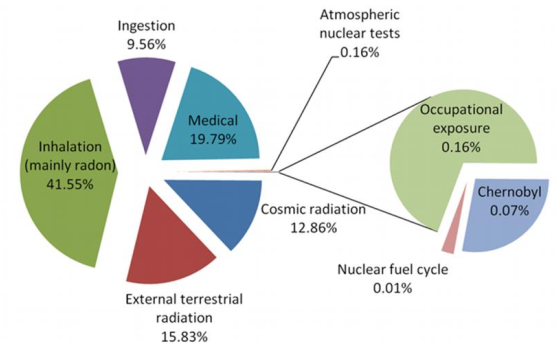
\includegraphics[scale=0.5]{2Introduction/RadioactiveDosePopulation.png}
\centering
\caption{Annual average distribution of the radioactive dose received by the population~\cite{IAEA}\label{fig:RadioactiveDosePopulation}.}
\end{figure}

\begin{table}[h]
\centering{}%
\begin{tabular}{lcc}
\toprule 
Radiation source & Eff. dose ($\milli\sievert/$yr) & Typical range ($\milli\sievert/$yr)\tabularnewline
\midrule
\midrule 
Cosmic (external) & $0.39$ & $0.3 - 1.0$ \tabularnewline
Terrestrial (external) & $0.48$ & $0.3-0.6$ \tabularnewline  
Inhalation (internal) & $1.26$ & $0.2-10$ \tabularnewline
Ingestion(internal) & $0.29$ & $0.2-0.8$ \tabularnewline
\midrule
Total & $2.42$ & $1-12.4$ \tabularnewline
\bottomrule
\end{tabular}
\caption{Annual average distribution of the effective dose received by the population due to natural radioactivity~\cite{UNSCEAR, CSN}.}
\label{tab:RadioactiveNaturalDosePopulation}
\end{table}

Since the discovery of radioactivity by Henri Becquerel in $1896$, lots of nuclear-based technologies were developed and applied to various fields such as Energy, Chemistry, Biology, Technology, Medicine, Industry, etc. Due to nuclear applications, a number of anthropogenic radioactive sources have emerged in society, resulting in radioactive elements released into the environment. It can be noticed in Figure \ref{fig:RadioactiveDosePopulation} that the most important part of the dose received by the population from artificial sources comes from medical practice. The growth of knowledge and the development of measurement techniques for radioactivity have provided evidence of the harmful effects of radioactivity on living organisms. This leads to the necessity of controlling the radiation to which the population is exposed, keeping it under safe limits. To accomplish this purpose, several organizations were created to propose recommendations for radiological protection to the different state organisms and governments at the international level. The main ones are:

\begin{enumerate}
\item{} The International Commission of Radiological Units and Measurements (ICRU) \cite{ICRU}, created during the first International Conference of Radiology held in London in 1925 to define concepts and units necessary to quantify the negative effects of radioactivity.

\item{} The International Commission on Radiological Protection (ICRP) \cite{ICRP}, created in 1928 by the International Society of Radiology (ISR) \cite{ISR}. The ICRP aims to make recommendations and provide guidance on different aspects of protection against radioactivity. The ICRP does not have the legal capacity to enforce its recommendations, but these are widely included in the legislation of most countries. %is fairly consistent with them.

\item{} The United Nations Scientific Committee on the Effects of Atomic Radiation (UNSCEAR) \cite{UNSCEAR}, created in 1955 with the goal of estimating and reporting the levels and effects of ionizing radiation on the population and the environment. These estimates are taken into account by governments worldwide to establish their safety standards.

\item{} The International Atomic Energy Agency (IAEA) \cite{IAEA}, created in 1957 to promote the peaceful use of nuclear energy and to avoid its use for military purposes such as nuclear weapons. Although established independently from the United Nations through its international treaty, the IAEA reports regularly to both the United Nations and the Security Council.

\item{} The European Atomic Energy Community (EURATOM), created in 1957, which is an international organization ruled by the EURATOM treaty. Its objective is to coordinate research programs for the peaceful use of nuclear energy and the sharing of knowledge, infrastructures and funding of nuclear energy.

\item{} The Nuclear Safety Council (CSN) \cite{CSN} of Spain, created in 1980, is the authority in Spain for nuclear safety and radiation protection. It has the objective of protecting employees, the general population and the environment from the harmful effects of ionizing radiation from anthropogenic origin. For this goal, the CSN ensures that nuclear and radioactive facilities are operated safely and establishes the preventive and corrective measures to be applied in radiological emergencies. The CSN manages two detector networks to control the levels of radioactivity in the environment and to assess the impact of radioactive facilities:

\begin{enumerate}
\item{} The network of automatic stations REA (Red de Estaciones Automáticas) \cite{REA}. The REA consists of several gamma detectors, distributed across the country as indicated in Figure \ref{subfig:REA}, which measure the radioactive dose in real time. The REA is employed for real-time detection of radiological issues to enable taking prompt safety measures.

\item{} The network of sampling stations REM (Red de Estaciones de Muestreo) \cite{REM}. The REM consists of a collection of points, shown in Figure \ref{subfig:REM}, from which samples are taken and measured in a laboratory. About twenty Spanish laboratories integrate this network. The objective of the REM is to characterize the concentration and evolution of radioisotopes present in the radioactive background of Spain and to quantify the impact of radioactive facilities on the environment.
\end{enumerate}

\begin{figure}
\centering
    \begin{subfigure}[b]{0.7\textwidth}
    \centering
    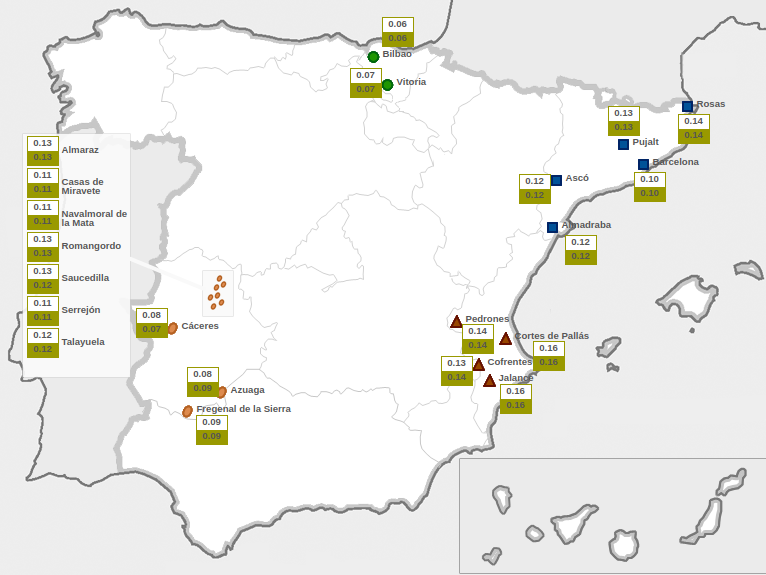
\includegraphics[width=\textwidth]{2Introduction/REA.png}  
        \caption{}\label{subfig:REA}
    \end{subfigure}
    \hfill
    \begin{subfigure}[b]{0.7\textwidth}
    \centering
    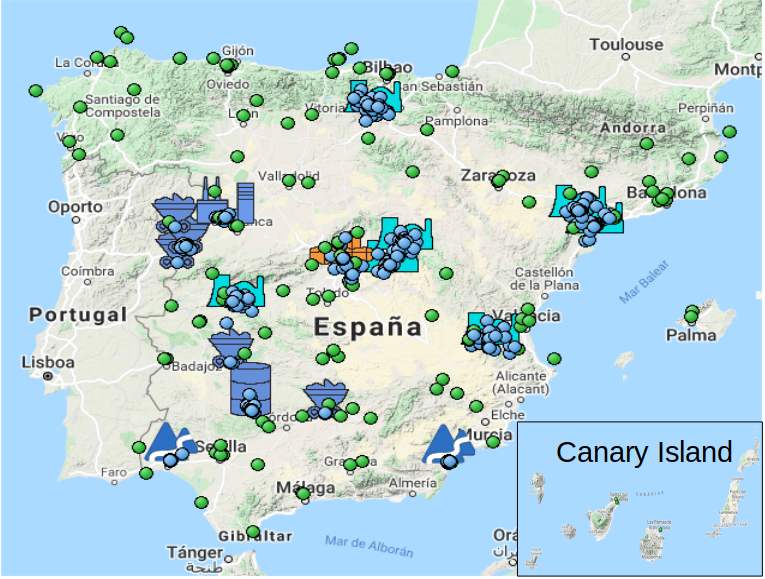
\includegraphics[width=\textwidth]{2Introduction/REM.png}  
    \caption{\label{subfig:REM}}
    \end{subfigure}
 \caption{Networks of automatic and sampling stations managed by the Spanish CSN. a) Measurement locations of the REA \cite{REA}. The white and green insets are the daily and monthly average of the gamma dose, respectively. b) Measurement locations of the REM \cite{REM}. Blue dots are locations near nuclear facilities, and green dots are locations uniformly distributed throughout the country.}
 \label{fig:NetworksCSN}
\end{figure}
%There are other networks that measure different parameters such as the concentration of $\ce{^{222}Ra}$ in the air. The measurements of all the networks complies with to the EUROTAM treaty \cite{100BqL}.

\end{enumerate}

The goal of the TRITIUM project is to develop a monitor capable of automatically measuring low levels of tritium in water in quasi-real-time\footnote{Quasi-real-time is an approximation of real-time measurements. It means a relatively small time, like less than $1~\hour$.}. This monitor is intended to be included in the REA.

Tritium is one of the radioactive isotopes routinely measured in REM tests. It is detected through the low-energy electrons produced in its beta decay, mainly using the Liquid Scintillation Counter technique (LSC). Due to the limitations of the current tritium detection techniques, described in section \ref{sec:StateOfTheArt}, the TRITIUM project was recently proposed with the objective of building a tritium detector based on scintillating fibres in contact with the water sample. The photons produced in these scintillating fibres are read out by photosensors, either photomultiplier tubes (PMTs) or silicon photomultipliers (SiPMs). The final emplacement of the TRITIUM monitor is a site close to the Arrocampo dam (Extremadura, Spain), whose water is used for the cooling system of the Almaraz nuclear power plant (NPP), located 4 km upstream from the Arrocampo dam. The monitor will be used to ensure that the tritium levels of the Arrocampo dam  water are below the legal limit of $100~\becquerel/\liter$ specified in the EURATOM Directive 2013/59/Euratom \cite{100BqL}. In addition, this will confirm the correct operation of the Almaraz NPP, since an increase of tritium activity released could indicate a malfunctioning of the reactor. This monitor could also be used in many different places with radioactive facilities like the future fusion power plants\footnote{The International Thermonuclear Experimental Reactor, ITER, will need up to several tens of kilograms of tritium to function, which corresponds to several $\tera\becquerel$ of activity.}, nuclear research facilities\footnote{Tritium is one of the main emissions from nuclear research facilities \cite{FERMILAB, BrookHavenNationalLaboratory}.} or tracking the pathway of tritium discharges to groundwater \cite{TrackingTritium}. 

Tritium is one of the most abundantly produced radioisotopes in an NPP, as it was verified in the United States Department of Energy (DOE) \cite{FiberDetector1a, FiberDetector1b}, in several research facilities in China \cite{CommonEmissionTritium} and places close to them (ground, surface and wastewater). Tritium is produced in the nuclear reactor cooling water system of NPPs by neutron capture of deuterium existing in the heavy water ($\ce{D_2 O}$), semi-heavy water ($\ce{H D O}$) or deuterium created by neutron capture in light water ($\ce{H_2 O}$). Tritium is finally released partially or totally into the environment in a quantity that depends on the reactor type, as shown in Table \ref{tab:TritiumEmisionsNPPs}. The most common form in which tritium is released into the environment is $\ce{HTO}$ \cite{CommonEmissionTritium}.
%All these processes have a large probability of happening due to the huge neutron flux, of the order of $10^{14} ~\ce{n} \, \cm^{-2} \second^{-1}$ in the nuclear reactor \cite{CrossSeccionNeutrons}

\begin{table}[htbp]
\centering{}%
\begin{tabular}{lcc}
\toprule 
Reactor type & Gaseous discharge ($\giga\becquerel/$y) & Liquid discharge ($\giga\becquerel/$y)\tabularnewline
\midrule
\midrule 
PWR & $3.70\cdot 10^{3}$ & $2.59\cdot 10^{4}$ \tabularnewline
BWR & $1.85\cdot 10^{3}$ & $3.70\cdot 10^{3}$ \tabularnewline
HWR & $7.40\cdot 10^{5}$ & $1.85\cdot 10^{5}$ \tabularnewline
GCR & $7.40\cdot 10^{3}$ & $1.11\cdot 10^{4}$ \tabularnewline
\bottomrule
\end{tabular}
\caption{Emission of tritium per year from different types of nuclear reactors: Pressurized Water Reactor (PWR), Boiling Water Reactor (BWR), Heavy Water Reactor (HWR) and Gas-Cooled Reactor (GCR) \cite{CommonEmissionTritium}.}
\label{tab:TritiumEmisionsNPPs}
\end{table}

NPPs are operational for more than 60 years and, nowadays, they are essential for providing a large part of the electric power used all over the world (more than $20\%$ in Spain \cite{PercentageEnergySpain} and more than $10\%$ in the world \cite{PercentageEnergyWorld}). Although the Spanish government is planning to progressively shut all NPPs down, there are other countries like China \cite{60ReactorsChina} or the United States \cite{35MillionsUSA} that promote their use. NPPs are a profitable investment since they are one of the cheapest sources of energy production. Their energy production rate is stable since it does not depend on meteorological conditions. Moreover, NPPs do not emit greenhouse gases. Although there are alternative energy sources which are being developed quickly (photovoltaic, wind, tidal energy, etc.), as well as other concepts of energy production and saving (local production, energy efficiency, smart cities, etc.), they are currently not enough to cover the population needs. However, NPPs have some important drawbacks such as contamination of fresh water from uranium mining, nuclear waste, nuclear proliferation and the risk of radioactive contamination from accidents as happened in the past: Chernobyl, Fukushima and Three Mile Island \cite{ThreeMileIsland}. In any case, world nuclear energy production is most likely not going to be stopped in the next decade. In fact, the United States Energy Information Administration (EIA) expects a future increase of nuclear energy production \cite{EIAOutlook}. Therefore, safety is not a negotiable aspect and there must be a development of safeguards, like alarm systems, that warn of any malfunction of NPPs. 

%which is normally done by liquid scintillation counter technic (LSC). This technic has a very good detection capability and precision but it has the inconvenient of providing a delayed results of about 1-2 days or even more. Liquid scintillation technique for the tritium measurement will be presented in section \ref{sec:StateOfTheArt}. 
	%\newpage
	
	\section{Tritium Properties and Radiological Hazards}\label{sec:TritiumProperties}
	Tritium is the only radioactive isotope of hydrogen. It was first time produced in $1934$ from neutron capture of deuterium by Ernest Rutherford, Mark Oliphant and Paul Harteck \cite{TritiumDiscovery} and it was first time isolated in 1939 by Luis Walter Alvarez and Robert Cornog \cite{TritiumIsolate}, who checked that tritium is a radiactive element. 

Tritium is naturally produced in the environment through the interaction of cosmics rays and gaseous elements of the upper atmosphere like nitrogen ($\ce{^{14}N}(\ce{n},\ce{^{3}H})\ce{^{12}C}$) \cite{TritiumHandling} and oxigen ($\ce{^{16}O}(\ce{n},\ce{^{3}H})\ce{^{14}N}$) \cite{OxigenTritium}. Around 99\% of this tritium form water (\ce{HTO}) and reaches the earth's surface as rain with an estimated produccion rate of $4\cdot 10^6 ~\curie/$yr ($1.48 \cdot 10^8 ~\giga\becquerel/$yr), producing a tritium concentration of $0.6-1.2~\becquerel/\liter$ in precipitation \cite{CommonEmissionTritium, TritiumHandling}. 

Tritium can be produced artificially in the environment from different anthropogenic sources \cite{CommonEmissionTritium, TritiumHandling}. There is a large amount of tritium which was produced in military nuclear test explosions between 1945 and 1975, with an estimated total production of $8 \cdot 10^9~\curie$ ($2.96 \cdot 10^{11}~\giga\becquerel$) and a part of which remains to the date. In these nuclear explosions, tritium was produced mainly from the nuclear reactions $\ce{^{14}N}(\ce{n},\ce{^{3}H})\ce{^{12}C}$ and $\ce{^{2}H}(\ce{n},\gamma)\ce{^{3}H}$. Tritium can be also produced by commercial producers of radioluminiscent and neutron generator devices ($1 \cdot 10^6~\curie/$yr), nuclear power and defense industries (around $2 \cdot 10^6~\curie/$yr) and several research facilities and nuclear reactor for energy production ($2 \cdot 10^6 \curie/\giga\watt$yr), whose main production cross sections are shown in Table \ref{tab:NuclearReactionsTritiumProduction}: 

\begin{table}[htbp]
\begin{center}
\begin{tabular}{|c|c|c|c|}
\hline
Element & Origin & Nuclear reaction & Cross section ($\barn$)\\
\hline \hline \hline
$\ce{^{2}_{1}H}$ & Water coolant & $\ce{^{2}_{1}H}(\ce{n},\gamma)\ce{^{3}_{1}H}$ & $5.2 \cdot{} 10^{-4}$ \\ \hline
$\ce{^{3}_{2}He}$ & Helium coolant & $\ce{^{3}_{2}He}(\ce{n},\ce{p})\ce{^{3}_{1}H}$ & $5330$ \\ \hline
$\ce{^{6}_{3}Li}$ & Moderator & $\ce{^{6}_{3}Li}(\ce{n},\alpha)\ce{^{3}_{1}H}$ & $940$ \\ \hline
$\ce{^{10}_{5}B}$ & \parbox{8em}{\centering Moderator,\\ control rods} & $\ce{^{10}_{5}B}(\ce{n},2\alpha)\ce{^{3}_{1}H}$ & $3835$ \\ 
\hline
\end{tabular}
\caption{Most common nuclear reactions of artificial tritium production~\cite{CommonEmissionTritium}}
\label{tab:NuclearReactionsTritiumProduction}
\end{center}
\end{table}

%\begin{equation}
%\ce{^{2}_{1}H}(\ce{n},\gamma)\ce{^{3}_{1}H} \qquad \sigma= 5.2 \cdot{} 10^{-4}~\barn  ~~~\cite{CommonEmissionTritium}
%\label{eq:capneuH2}
%\end{equation}

%\begin{equation}
%\ce{^{3}_{2}He}(\ce{n},\ce{p})\ce{^{3}_{1}H} \qquad \sigma= 5330~\barn ~~~\cite{CommonEmissionTritium}
%\label{eq:capneuHe3}
%\end{equation}

%\begin{equation}
%\ce{^{6}_{3}Li}(\ce{n},\alpha)\ce{^{3}_{1}H} \qquad \sigma= 940~\barn ~~~\cite{CommonEmissionTritium}
%\label{eq:capneuLi6}
%\end{equation}

%%\begin{equation}
%%\ce{^{7}_{3}Li}(\ce{n},\alpha)\ce{^{3}_{1}He} + \ce{n} ~~~\cite{CommonEmissionTritium}
%%\label{capneuLi7}
%%\end{equation}

%\begin{equation}
%\ce{^{10}_{5}B}(\ce{n},2\alpha)\ce{^{3}_{1}H} \qquad \sigma= 3835~\barn ~~~\cite{CommonEmissionTritium}
%\label{eq:capneuB10}
%\end{equation}

%\begin{equation}
%\ce{^{11}_{5}B}(\ce{n},2\alpha)\ce{^{3}_{1}H} + n ~~~\cite{CommonEmissionTritium}
%\label{capneuB11}
%\end{equation}
%$\eqref{capneuLi6}$ para referenciar ecuaciones

%There are two more nuclear reaction with which we can produce tritium:

%\begin{equation}
%\ce{^{1}_1 H} (2 \cdot{} \ce{n},\ce{p})\ce{^{3}_1 H}
%\label{doblecapneuH}
%\end{equation}

%\begin{equation}
%\ce{^{2}_1 H}(\ce{n},\gamma)\ce{^{3}_1 H}
%\label{capneuD}
%\end{equation}

Tritium levels in the environment when anthropological radioactive sources are not involved are between $1$ and $4~\becquerel/\liter$. This is a higher value than the expected due to the cosmogenic background levels ($0.6-1.2~\becquerel/\liter$, previously mentioned) \cite{FranceTritiumEnvironment}. It can be explained by the consequences of nuclear weapons tests.

Tritium levels in rivers around a nuclear facility are between $1$ and $10~\becquerel/\liter$ and even between $20$ and $50~\becquerel/\liter$ at the water discharge site of NPPs \cite{FranceTritiumEnvironment}, where the produced tritium is partially or totally released into the environment, mainly in the $\ce{HTO}$ water form.

The effect of NPP on tritium levels can be observed using the public measurements of the REM, explained in the section \ref{sec:Introduction}. For example, in the case of Cofrentes, which is the closest nuclear power plant to Valencia and the one in whose measurements are involved LARAM\footnote{LARAM is a Valencia laboratory specialized in environmental radioactivity measurements}, the tritium levels in the river are measured in three different places, marked on the map shwon in Figure \ref{fig:SamplingLocations}. The first place, P1, is located in the river, $6~\kilo\meter$ upstream from the NPP, the second place, P2, is located $1~\kilo\meter$ downstream and the third place, P3, is located $5~\kilo\meter$ downstream. The level of Tritium measured in these three locations is shown over time in Figures \ref{fig:TritiumL6kB}, \ref{fig:TritiumL1kA} and \ref{fig:TritiumL5kA} respectively.

\begin{figure}[hbtp]
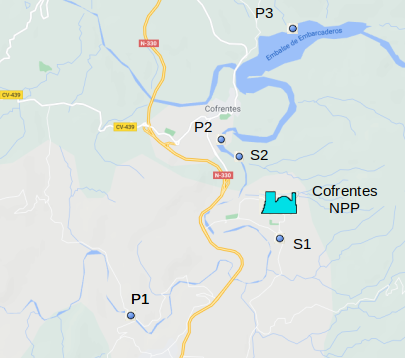
\includegraphics[scale=0.5]{2Introduction/CofrentesMaps.png}
\centering
\caption{Tritium sampling locations around Cofrentes NPP.\label{fig:SamplingLocations}}
\end{figure}

\begin{figure}[hbtp]
 \centering
  \subfloat[Tritium activity $6~\kilo\meter$ upstream.]{
  \label{fig:TritiumL6kB}
    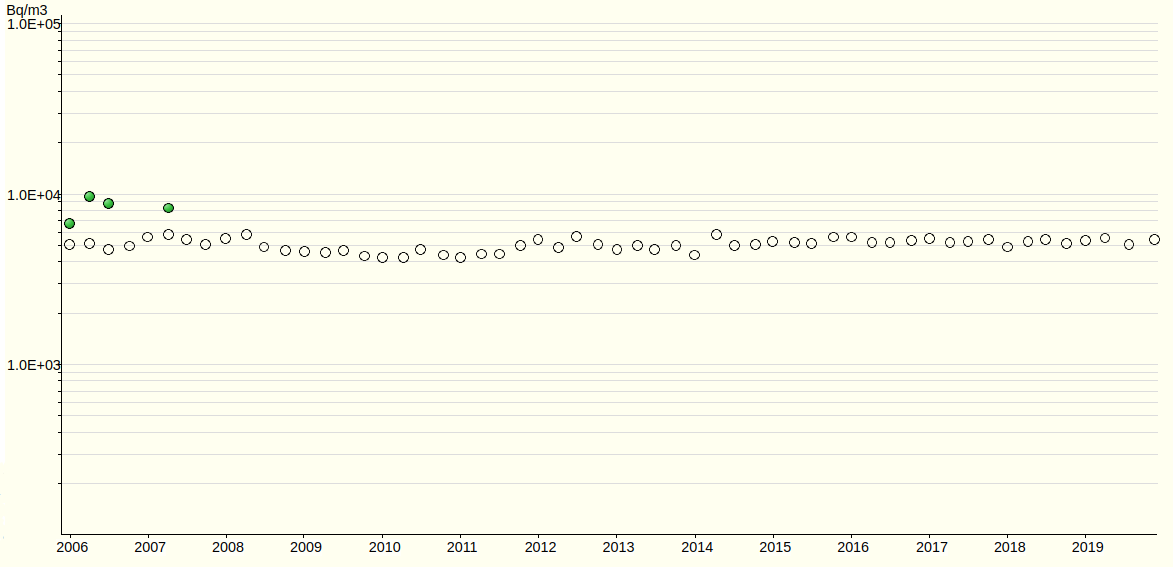
\includegraphics[width=0.47\textwidth]{2Introduction/6km_before.png}}
    %\newline
      \subfloat[Tritium activity $1~\kilo\meter$ downstream.]{
   \label{fig:TritiumL1kA}
    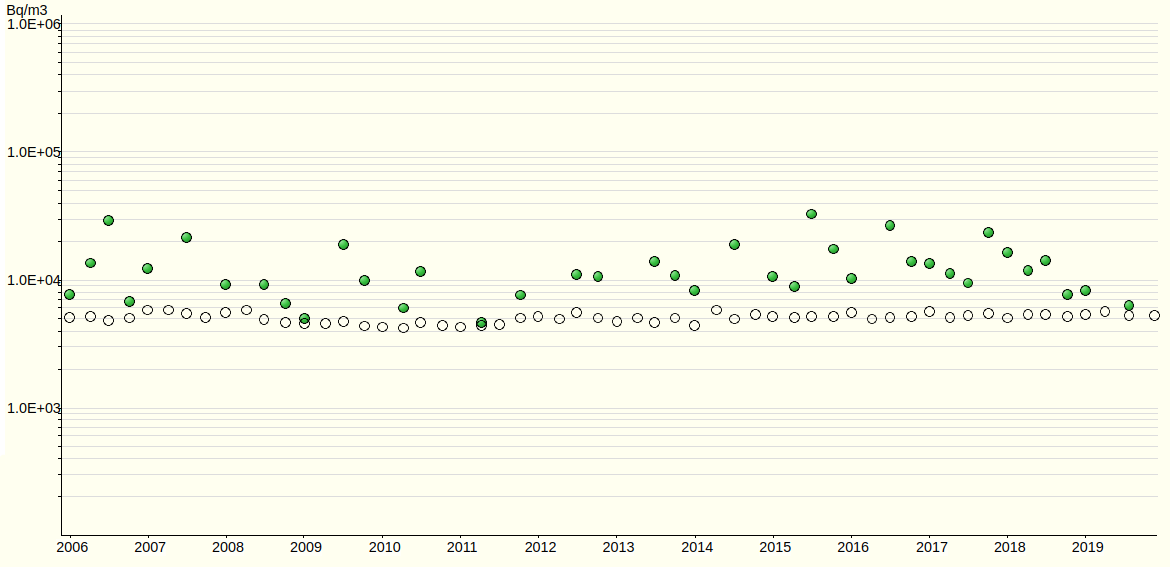
\includegraphics[width=0.47\textwidth]{2Introduction/1km_after.png}}
    \newline
  \subfloat[Tritium activity $5~\kilo\meter$ downstream.]{
  \label{fig:TritiumL5kA}
    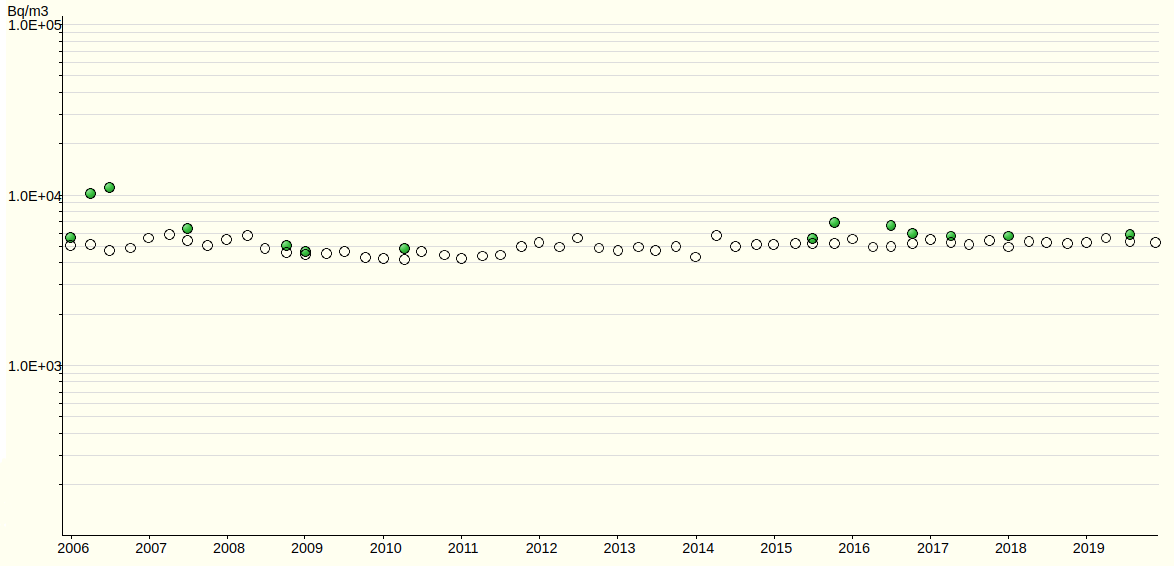
\includegraphics[width=0.47\textwidth]{2Introduction/5km_after.png}}
 \caption{Tritium activity levels in surface water around Cofrentes NPP from January $2006$ to November $2019$. The white points are used for the detection limit and the green points are used for the measured activity, when it is above the detection limit.~\cite{REM}}
 \label{fig:MeasurementsCofrentesSurface}
\end{figure}

In these figures, the detection limit and the measured activity are shown using white dots and green dots respectively. The measured activity is only displayed when it is larger than the corresponding detection limit. As it can be seen, the tritium level in the river increases due to the discharge of the NPP and it is diluted again after $4~\kilo\meter$ downstream. 

Two additional measurements of the tritium level in groundwater have been included, points S1 and S2 on the map in Figure \ref{fig:SamplingLocations}, which are located $1~\kilo\meter$ before and $1~\kilo\meter$ after the NPP. Both tritium levels are shown in the figure \ref{fig:TritiumLG1kB} and \ref{fig:TritiumLG1kA} respectively, where it can be verified that the nuclear power plant has not affected them.

\begin{figure}[hbtp]
 \centering
      \subfloat[Tritium activity $1~\kilo\meter$ before NPP.]{
   \label{fig:TritiumLG1kB}
    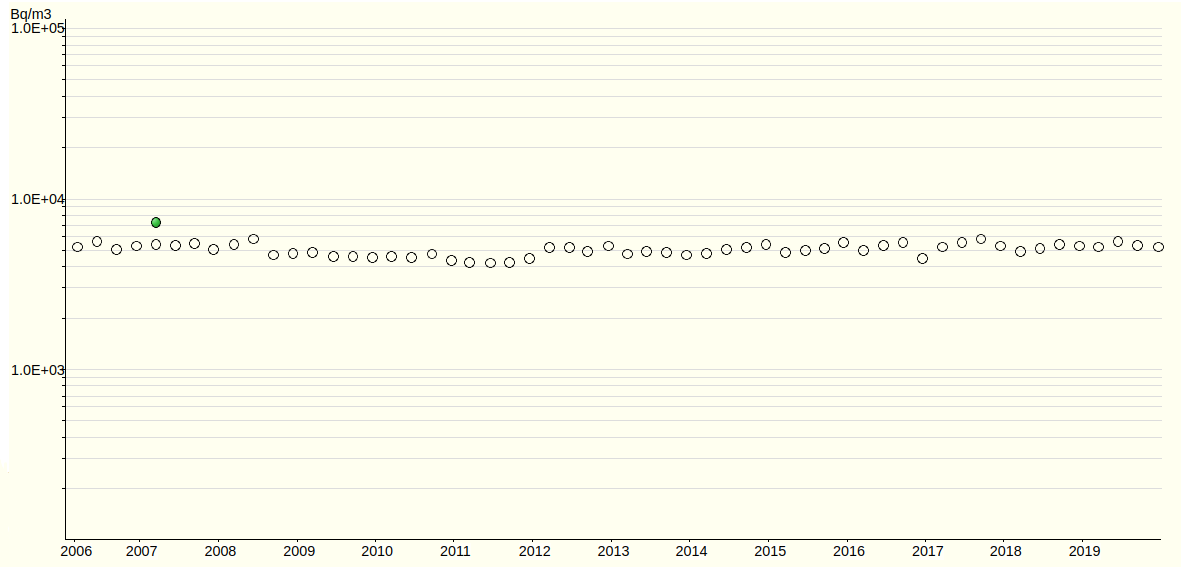
\includegraphics[width=0.47\textwidth]{2Introduction/Subterranea_before.png}}
    %\newline
  \subfloat[Tritium activity $1~\kilo\meter$ after NPP.]{
  \label{fig:TritiumLG1kA}
    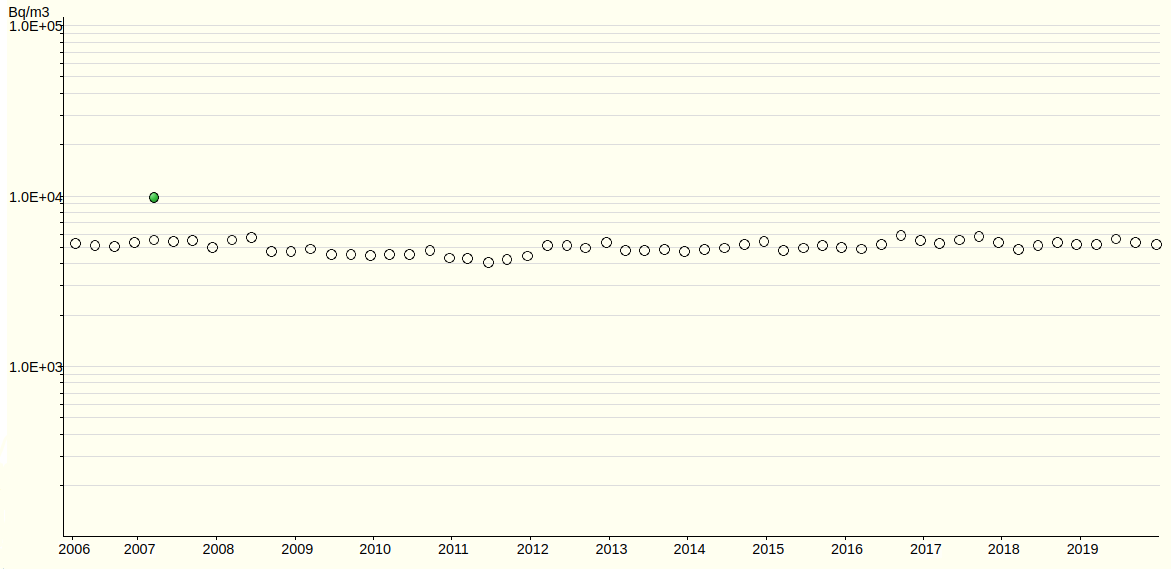
\includegraphics[width=0.47\textwidth]{2Introduction/Subterranea_1_km_later.png}}
 \caption{Tritium activity levels in groundwater around Cofrentes NPP from January $2006$ to November $2019$.~\cite{REM}}
 \label{fig:MeasurementsCofrentesGroundWater}
\end{figure}

It is important to note that, although environmental tritium levels have been affected due to NPP, these levels are below the legal limit. The maximum level of tritium measured since of January 2, 2006 is around $32~\becquerel/\liter$, below to the legal limit in Europe, $100~\becquerel/\liter$.

Tritium is a radioactive element whose half-life time is $T_{1/2}= 12.32$ years. It has one proton and two neutrons and decays exclusively through $\beta$ radiation. It decay $100\%$ directly to the ground state of Helium ($\ce{^{3}_{2}He}$), which is a stable nuclei, thorugh the decay scheme of equation \ref{eq:TritiumDecay}:

%In this decay, one neutron of tritium is transformed transformed into a proton, an electron and an electron-antineutrino, according to the following decay scheme:

%\begin{equation}
%\ce{n} \longrightarrow \ce{p}  + \ce{e^-}  + \ce{\overline{\nu}_e}
%\label{eq:BetaDecay}
%\end{equation}



\begin{equation}
\ce{^{3}_{1}H} \longrightarrow \ce{^{3}_{2}He}  + \ce{e^-}  + \ce{\overline{\nu}_e}
\label{eq:TritiumDecay}
\end{equation}

In Figure \ref{fig:TritiumDecay} the scheme of tritium energy levels is shown. In this decay it is not possible to detect the neutrino because of its extremely weak interaction with matter ($\sigma \propto 10^{-42} ~ \cm^2$ \cite{CrossSeccionNeutrino}) and, since $\ce{^{3}He}$ has a much larger mass than electrons and neutrinos, by conservation of energy and momentum, the energy that is taken by this daughter nucleus is very small. Therefore, the detection of tritium is through its decay electron. 

\begin{figure}[hbtp]
 \centering
  \subfloat[Tritium energy levels \cite{TritiumDecayEnergyLevels}]{
   \label{fig:Energy_levels}
    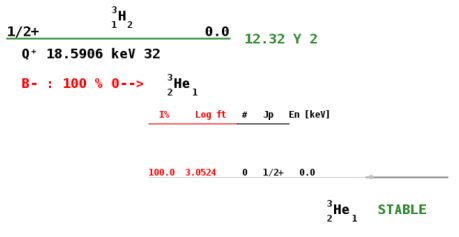
\includegraphics[width=0.60\textwidth]{2Introduction/esquema_niveles_energeticos.png}}
  \subfloat[Graphic representation of tritium decay \cite{TritiumDecayImage}]{
   \label{fig:GraphicDesintegration}
    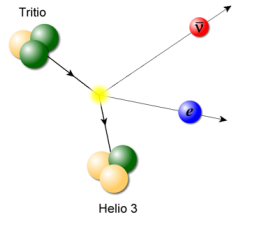
\includegraphics[width=0.40\textwidth]{2Introduction/representacion_desintegracion.png}}
 \caption{Tritium decay}
 \label{fig:TritiumDecay}
\end{figure}

The energy released in the tritium decay is $Q_\beta=18.6~\keV$, which is divided between the decay products. Therefore, the energy spectrum of the decay electrons is a continuum with a maximum value of $18,6~\keV$, as shown in Figure \ref{fig:TritiumDecaySpectrum}. This energy spectrum has an average of $5.7~\keV$ and the most likely value is slightly below, around $4.5~\keV$.

\begin{figure}[hbtp]
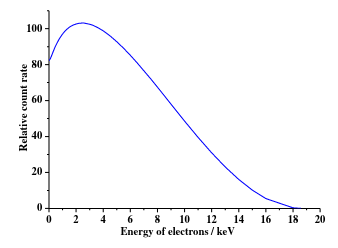
\includegraphics[scale=0.6]{2Introduction/Espectro_tritio.png}
\centering
\caption{Energy spectrum of tritium electrons ~\cite{TritiumEspectrum}\label{fig:TritiumDecaySpectrum}}
\end{figure}

%We have to keep in mind that, although the helium isotope is stable, it will be exited immediately after this decay. As a consequence, after the tritium $\beta^-$ decay, we will have a subsequent dexcitation of the $\ce{^{3}He}$ which will produce photons, $\gamma$, with several well-defined energies that correspond to their energy levels, X-rays\footnote{X-rays are photons whose wavelength are between 0.01 nm and 10 nm. They are produced by nuclear deexitation.}. It will not affect our tritium measurement because, as we will see in Section  \ref{}, the probability of detecting X-rays with the photosensor that will be used is practically negligible.

%Los rayos X son una radiación electromagnética de la misma naturaleza que las ondas de radio, las ondas de microondas, los rayos infrarrojos, la luz visible, los rayos ultravioleta y los rayos gamma. La diferencia fundamental con los rayos gamma es su origen: los rayos gamma son radiaciones de origen nuclear que se producen por la desexcitación de un nucleón de un nivel excitado a otro de menor energía y en la desintegración de isótopos radiactivos, mientras que los rayos X surgen de fenómenos extranucleares, a nivel de la órbita electrónica, fundamentalmente producidos por desaceleración de electrones. La energía de los rayos X en general se encuentra entre la radiación ultravioleta y los rayos gamma producidos naturalmente. Los rayos X son una radiación ionizante porque al interactuar con la materia produce la ionización de los átomos de la misma, es decir, origina partículas con carga (iones). 

The releasing energy of the tritium decay, is very little. In fact, it is the radioactive isotope with the lowest energy released in its $\beta$ disintegration \cite{TritiumHandling}. Consequently, the $\beta$ particle which is emitted in this tritium decay will have a very small mean free path as it is shown in Table \ref{tab:MeanFreePathTritium}.

\begin{table}[htbp]
\begin{center}
\begin{tabular}{|c|c|c|}
\hline
Material & P. Depth ($5.7~\keV$) & P. Depth ($18.6~\keV$)\\
\hline \hline \hline
$\ce{\ce{^{3}_{1}H_2}}$ & 0.26 cm & 3.2 cm \\ \hline
Air & 0.036 cm & 0.45 cm \\ \hline
\parbox{10em}{\centering Water, soft tissue\\  (solid matter whose \\  density is $1~\gram\cdot\cm^{-3}$)} & 0.42 $\mu\meter$ & 5.2 $\mu\meter$ \\ \hline
\end{tabular}
\caption{Penetration depth for decay electron of mean ($5,7~\keV$) and maximum ($18,6~\keV$) energies in different media (tritium gas and air at standard conditions of temperature ($273~\kelvin$) and preassure ($1$ atm), STP, and water)~\cite{MeanFreePathDocument}}.
\label{tab:MeanFreePathTritium}
\end{center}
\end{table}

This short mean free path is a major issue in tritium detection, as it makes more difficult the electron detection, which will require a highly sensitive detector. However, it means that the tritium electrons has a low penetration in our body and easily stopped with our clothes or laboratory gloves, resulting in a low radiological hazard of external tritium.

Nevertheless, the danger of tritium increases when it is ingested or inhaled since it can bind anywhere that hydrogen can and perform the same chemical reactions, sometimes with higher rate if the tritium concentration is high enough to catalyze the reaction. 

Tritium can be absorbed in our body in three different ways, gaseous tritium (mainly HT), tritiated water (mainly HTO) and organically bound tritium (called OBT).

The gaseous tritium, which is normally found mixed in the air, is the least important since less than a $3-5 \cdot{} 10^{-3}~\%$ is absorbed, which is insignificant \cite{TritiumHandling}. However, it can be transformed into tritiated water through the oxidation and exchange reactions shown in the chemical schemes of equations \ref{eq:OxidationExchange}, which has a more important effect on health \cite{TritiumHandling}:

\begin{equation}
\begin{split}
& Oxidation: \qquad \qquad \qquad \qquad \qquad \qquad Exchange\\
& 2\cdot{}\ce{HT} + \ce{O_2} \rightarrow 2 \cdot{} \ce{HTO} ~ \quad \qquad \qquad \qquad \ce{HT} + \ce{H_2 O} \rightarrow \ce{H_2} + \ce{HTO}\\
& 2\cdot{}\ce{T_2} + \ce{O_2} \rightarrow 2 \cdot{} \ce{T_2 O} \qquad \qquad \qquad \qquad \ce{T_2} + \ce{H_2 O} \rightarrow \ce{HT} + \ce{HTO}
\label{eq:OxidationExchange}
\end{split}
\end{equation}

Tritiated water, which is normally found in drinking water or water in food, has a larger impact since the $99\%$ of it is absorbed \cite{TritiumHandling}. In addition, its biological life time of it is around $9.5$ days ($\pm50\%$), time during which tritium will remain in our body \cite{TritiumHandling, FranceTritiumEnvironment, EstimationTritiumDosi}.

This time corresponds to the water cycle in the body and, like this, it can vary due to various external parameters such as temperature, humidity, drinking habits, etc. or reduced with the use of diuretics \cite{TritiumHandling}.

Organically bound tritium, normally found in food, generally forms a covalent bond with a carbon and and it corresponds to $5-10~\%$ of tritium absorbed in the body. Although it is absorbed in less quantity in the body than tritiated water, it can be more dangerous since it has a longer biological life time. The biological life time of this tritium type depends on the affinity of the organic molecule with the different biological tissues and it can vary from tens of days to hundreds of days (larger than the ICRP estimate) \cite{FranceTritiumEnvironment, EstimationTritiumDosi, EstimationTritiumDosiRats, EstimationTritiumDosiKangarooRats}.

There are many studies showing that tritium in living matter can cause the same effects than X-rays or $\gamma$ rays, which are mutations, tumors, cancer, genetic effects, reproductive effects, etc \cite{StraumeTritiumHazard, RytoemaaTritiumHazard}. In fact, the consequences of tritium radiation can be worse than a similar $\gamma$ radiations since its biological efficiency\footnote{The biological efficiency is used to quantify the damage produced in the living cells due to an external radiation.} is two or three times larger \cite{StraumeTritiumHazard}.

In summary, tritium is a naturally occurring radioactive element that can affect health if it is released excessively. Because of that, each country has developed a legislation, shown in section \ref{sec:Legislation}, to manage the release of tritium and ensure that these background levels are safe for health.



%Tritium has different physical properties than other natural isotopes of the hydrogen like different boiling points as shown in Table \ref{tab:BoilingPoints} or the property of self-radiolysis which only happens when radioactive elements are involved. In the case of tritium dissolved in water, it is normally found forming the $\ce{HTO}$ molecule. There, the auto-radiolysis ocurrs because the energy released in tritium decay is larger than the energy bond of oxigen and hydrogen in water molecules ($5.2~\eV$) or the ionization energy of water molecules ($12.6~\eV$) so it can break up these molecules \cite{AutoRadyolisis}. Due to the auto-radiolysis, some radicals appear in the water, increasing its corrosivity. It is a fact that we have to take into account when choosing the materials that will make up the TRITIUM detector.

%\begin{table}[htbp]
%\begin{center}
%\begin{tabular}{|l|l|l|}
%\hline
%Molecule & Boiling point (for gases) ($\kelvin$) & oxidation form\\
%\hline \hline \hline
%$\ce{H_2}$ & 20.39 & $\ce{H_2 O}$ \\ \hline
%$\ce{HD}$ & 22.14 & $\ce{HDO}$ \\ \hline
%$\ce{HT}$ & 22.92 & $\ce{HTO}$ \\ \hline
%$\ce{D_2}$ & 23.66 & $\ce{D_2 O}$ \\ \hline
%$\ce{DT}$ & 24.38 & $\ce{DTO}$ \\ \hline
%$\ce{T_2}$ & 25.04 & $\ce{T_2 O}$ \\ \hline
%\end{tabular}
%\caption{Gas molecules of hydrogen isotopes and their boiling point and oxidation form.~\cite{}}
%\label{tab:BoilingPoints}
%\end{center}
%\end{table}

%Although tritium has different physical properties it has almost the same chemical behaviour than other hydrogen isotopes. Tritium, like hydrogen, is a gas at STP forming a two-atom molecules which can be $\ce{HT}$, $\ce{DT}$ and $\ce{T_2}$. 


%Due to this chemical similarity tritiated water can perform the same chemical processes than non-radiactive water, sometimes with higher rate if the tritium concentration is high enough to catalyze the reaction. Its biological hazard comes from this chemical similarity since tritiated water is able to substitute normal water in human body. 

	%\newpage
	
	\section{Current Legislation}\label{sec:Legislation}
	Due to the radiological risk of tritium, which has been shown in section \ref{sec:TritiumProperties}, it is important to develop a legislation that limits the release of tritium to the environment ensuring that the levels are below a safe value for health.

The guidelines that impose the limit of radioactive elements in drinking water for many countries are based on the radiation protection methodology developed by the ICRP \cite{ICRP_GL} and the recommendations of the world health organization, WHO \cite{WHO_GL}.

The objective of the international radiation methodology is to  protect people and the environment from the negative effects of ionizing radiations without limiting beneficial activities that involve radiation exposure. It is based on three main points, which are the justification (the benefit from radiological exposure must outweigh the detriment to health that it causes), the ALARA principle, "As Low As Reasonably Achievable" (the radiological exposure must be kept as low as possible considering social and economic factors) and dose limitation (limit that must never be exceeded).

While the ICRP recommends a maximum dose of $1~\milli\sievert/$yr, excluding the natural background and medical interventions, the WHO is more conservative, recommending a maximum dose of $0.1~\milli\sievert/$yr, which correspond to less than $5\%$ of the annual dose due to background radiation, $2.42~\milli\sievert/$year, Table \ref{tab:RadioactiveNaturalDosePopulation}.

The guideline reference level of each radionuclide in drinking water, GL, is usually calculated from these recomendations using the equation \ref{eq:Guideline}

\begin{equation}
GL = \frac{RDL}{DCF \cdot{} q}
\label{eq:Guideline}
\end{equation}

Where RDL is the reference dose level, DCF is the dose conversion factor (the normal used value for tritium is $1.8*10^{-11}~\sievert\becquerel$, provided by ICRP \cite{ICRP_factor}) and q is an estimation of the annual volume of drinking water consumed (normally assumed two liters per day, $730~\liter/$yr).

The GLD calculated for tritium in drinking water according to the ICRP and WHO recommendations is $76103~\becquerel/\liter$ and $7610~\becquerel/\liter$  respectively. It means that tritiated water with activities below these values is not harmful to health.

Based on these recommendations, each country has created organizations in charge of developing its own legislation on radionuclide limits. In Spain, the responsible organization of this task is the CSN.

Most of the countries in the world implement the RDL of $0.1~\milli\sievert/$yr recommended by the WHO. The legal limit for tritium in drinking water in this case is $76.103~\becquerel/\liter$  but it is often approximated in different ways. Some countries like Switzerland \cite{Switzerland_GL} or some organizations like the WHO \cite{WHO_GL} rounded this value to $10,000~\becquerel/\liter$. Others like some countries of Canada, such as Ontario and Québec, truncate this value to the first number $7,000~\becquerel/\liter$ \cite{Ontario_GL, Quebec_GL}. There are other countries like Russia which use the much more accurate approximation value of $7,700~\becquerel/\liter$ \cite{Russia_GL}.

There are other countries like Australia that prefer to implement the RDL of $1~\milli\sievert/$yr, recommended by the ICRP, whose legal limit is $76.103~\becquerel/\liter$ \cite{Australia_GL}. Other countries like Finland are based in the ICRP recommendations and use only the middle of this value, $0.5~\milli\sievert/$yr, whose value is rounded to a legal limit of $30,000~\becquerel/\liter$ for tritium in drinking water \cite{Finland_GL}.

There are two different exceptions to these recommendations:
\begin{enumerate}
\item{} On the one hand, most of the USA countires, such as California, use a RDL of $4~\milli\rem~(0.04~\milli\sievert)$, which corresponds to a legal limit of $20~\nano\curie/\liter~(740~\becquerel/\liter)$ \cite{California_GL}. This value was proposed by the United States Environmental Protection Agency (US EPA) as a result of an analysis of the available information \cite{USEPA_GL}.

\item{} On the other hand, most of the EU countries, such as France, Germany or Spain, impose an GL of $100~\becquerel/\liter$, which is one of the most restrictive limit in the world \cite{France_GL, Germany_GL, Spain_GL}. This value arise from the consideration that it is an indicator of the presence of other radionuclides more dangerous than tritium. These limits are fixed by the EURATOM Council Directive \cite{EURATOM_GL}. 
\end{enumerate}

All limits mentioned in this section are summarized in table \ref{tab:LegalLimitTritium}.

\begin{table}[htbp]
\begin{center}
\begin{tabular}{|c|c|}
\hline
Country/Agency & Legal limit of tritium ($\becquerel/\liter$)\\
\hline \hline \hline
ICRP & $76,103$ \\ \hline
WHO & $10,000$ \\ \hline
Switzerland & $10,000$ \\ \hline
Canada & $7,000$ \\ \hline
Russia & $7,700$ \\ \hline
Australia & $76,103$ \\ \hline
Finland & $30,000$ \\ \hline
United States & $740$ \\ \hline
European Union & $100$ \\ \hline
\end{tabular}
\caption{Legal limit of tritium in drinking water stablished in each country.}
\label{tab:LegalLimitTritium}
\end{center}
\end{table} 
	%\newpage
	
	\section{This Thesis}\label{sec:ThisThesis}
	This thesis is divided into nine different chapters that structure the information as follows:

\begin{enumerate}
\item{} \textbf{Chapter 1} provides a brief introduction to tritium detection, reports some important properties of tritium, and discusses the current legislation that limits tritium levels for human consumption in many countries around the world. 

\item{} \textbf{Chapter 2} describes the State-of-the-Art of tritium detection and shortly introduces the TRITIUM project. 

\item{} \textbf{Chapter 3} outlines the different parts of the TRITIUM monitor, which are the ultrapure water system, the background rejection system (consisting of the lead shielding and the active veto)  and the tritium detector. 

\item{} \textbf{Chapter 4} reports the calibrations of the different parts of the TRITIUM monitor and describes the developments aimed at improving the efficiency of tritium detection. 

\item{} \textbf{Chapter 5} details the geometrical configuration of the different prototypes built in the TRITIUM project. 

\item{} \textbf{Chapter 6} details the Monte Carlo simulations performed in the TRITIUM project. 

\item {} \textbf{Chapter 7} and \textbf{Chapter 8} report the results  achieved for the built prototypes and the simulations carried out, respectively. 

\item{} \textbf{Chapter 9} summarizes the most important results achieved in this work.

\end{enumerate}


	\newpage
	
\chapter{Methods of Detection of Tritium In Water}\label{chap:TritiumDetection}
%\chaptermark{Methods of Tritium Detection}
	
	\section{Tritium Detection State-of-the-Art}\label{sec:StateOfTheArt}
	Measurement of tritium activity is one of the routine environmental controls that are carried out in the vicinity of nuclear research facilities and nuclear power plants during their energy production lifetime. This measurement is carried out with different available technologies according to the state of the art of tritium detection. The most employed techniques are summarized in Table \ref{tab:DifferentThecnics}. Nowadays, the most used technique for measuring tritium in water is liquid scintillator counting (LSC). This technique consists of mixing a liquid sample (some millilitres for environmental measurements or less for higher activities) with liquid scintillator. This mixture is usually made in a ratio of 50:50 but it depends on the detection system and the activity of the samples \cite{LSCothers, Hofstetter1}. In this technique, the $\beta$ particles emitted from the sample excite the molecular energy levels of the liquid scintillator which promptly decays emitting several photons with a well-known energy (fluorescence), usually in the visible spectrum. Finally, these photons are detected with photosensors which convert the optical signal into a measurable electrical charge. The liquid scintillator technique has a very good detection sensitivity for low activity levels of tritiated water ($<1~\becquerel/\liter$) \cite{0.6Bq_L} but has the disadvantage of long measurement time (up to 2 days) and production of chemical waste, since liquid scintillators contain toluene which is toxic. In addition, the LSC technique requires special staff for sampling, a chain of custody and laboratory analysis which require economic and time resources. In order to overcome these difficulties, efforts were made to build a tritium monitor based on LSC which did not led a low enough minimum detectable activity (MDA) \cite{OnlineLSC}. 

{\renewcommand{\arraystretch}{1.8}
\begin{table}[htbp]
\centering{}%
\begin{tabular}{lcccc}
\toprule 
 & LSC & IC & Calorimetry & BIXS \tabularnewline
\midrule
\midrule 
\parbox{5em}{Measured\\ quantity} & \parbox{5em}{\centering Scintillation\\ photons} &  \parbox{5em}{\centering Ionization\\ current} & Heat & X-rays \tabularnewline
MDA & $\sim\becquerel$ & $10-100~\kilo\becquerel$ & $\sim~\giga\becquerel$ & $\sim~\mega\becquerel$ \tabularnewline
Sample state & Liquid & Gas, vapor & All & All \tabularnewline
\bottomrule
\end{tabular}
\caption{State-of-the-art tritium detection techniques. This table shows the measured quantity, the minimum detectable activity (MDA) and the sample form for four different techniques, liquid scintillator counting (LSC), ionization chamber (IC), calorimetry and beta induced X-ray spectrometry (BIXS).}
\label{tab:DifferentThecnics}
\end{table}}

The ionization chamber technique (IC) consists of an ionization chamber filled with gas (sample) which contains electrodes that collect the ionization current produced by the $\beta$ radiation in the gas. This is a simple and fast system, but it has a high MDA ($> 10~\kilo\becquerel$) and requires samples in a state of gas or steam \cite{IonizationChamber1, IonizationChamber2}. The IC technique also requires sample conditioning, chain of custody and laboratory analysis. 

The calorimetry method is based on the measurement of the heat generated in the detection medium (normally platinum) \cite{Calorimeter1, Calorimeter2}. The disadvantages of this technique are its high MDA (of the order of a $\giga\becquerel$) and the requirement of a long measurement time (2 days or more).

The Beta Induced X-ray Spectrometry (BIXS) is based on the measurement of the bremsstrahlung radiation produced by tritium decay electrons by a \ce{NaI(Tl)} crystal coupled to a PMT  \cite{XRays1, XRays2} or silicon drift detector (SDD) \cite{Bremstrahlung}. The limitation of this technique is its high MDA (of the order of $\mega\becquerel$).

There are additional methods for tritium detection, although they are less employed or less developed, each one with its advantages and limitations. For example, the avalanche photodiode (APD) cannot be used in contact with water \cite{APD},  the mass spectrometry needs to store the sample for several months \cite{Spectrometry} and the cavity ring spectroscopy requires a special optical configuration that is not possible outside a laboratory \cite{Ring}.

All the above techniques are offline methods that need a long time for sample collection, shipment to a laboratory and activity measurement. Therefore, they cannot be used for in-situ monitoring of tritium in water. The liquid scintillation technique is the only one with an MDA smaller than the requirement of $100~\becquerel/\liter$ of tritium in water established by the EURATOM directive. 

The purpose of the TRITIUM project is to develop an alternative method, based on solid scintillators, that allows accomplishing the requirements of in-situ monitoring of levels as low as $100~\becquerel/\liter$ in quasi-real-time. There are several studies with solid scintillators so far:

\begin{enumerate}

\item{} The study by M. Muramatsu, A. Koyano and N. Tokunaga in 1967 used a scintillator plate read out by two PMTs in coincidence \cite{Muramatsu}.

\item{} The study by A. A. Moghissi, H. L. Kelley, C. R. Phillips and J. E. Regnier in 1969 used one hundred plastic fibres coated with anthracene powder and read out by two PMTs in coincidence \cite{Moghissi}.

\item{} The study by R. V. Osborne in 1969 used sixty stacked scintillator plates read out by two PMTs in coincidence \cite{Osborne}.

\item{} The study by A. N. Singh, M. Ratnakaran and K. G. Vohra in 1985 used a scintillator with several holes read out by PMTs in coincidence \cite{Ratnakaran, Ratnakaran2000}.

\item{} The study by K. J. Hofstetter and H. T. Wilson in 1991 tested different shapes of scintillator plastics like several sizes of beads, fibres, etc. The best result obtained for solid plastic scintillators was a tritium detection efficiency, $\varepsilon_{det}$, of the order of $10^{-3}(\liter\second^{-1}\kilo\becquerel^{-1})$ \cite{Hofstetter1, Hofstetter2}.

\end{enumerate}

The results of those studies are summarized in Table \ref{tab:PlasticScinTritium}. As the active surface of the plastic scintillator $F_{sci}$ varies largely with the detector type, the specific detector efficiency $\eta_{det}$, which is the intrinsic efficiency normalized to its active surface, is used to compare the results. Finally, the MDAs in those studies are of the order of a few tens of $\kilo\becquerel/\liter$. The development of a detector with a much lower MDA is thus essential to comply with the EURATOM directive of 100 Bq/L of tritium in water for human consumption.

\begin{table}[htbp]
\centering{}%
\begin{tabular}{lcrcc}
\toprule 
Reference & \parbox{5em}{$\eta_{det}\times10^{-3}\\\liter~\kilo\becquerel^{-1}\second^{-1}$}  & \parbox{3.5em}{\raggedleft $F_{sci}$\\ $\cm^2$}  & \parbox{6.5em}{$~S_{det}\times 10^{-6}\\\liter~\kilo\becquerel^{-1}\second~\cm^{-2}$} &  \parbox{3.5em}{MDA\\$\kilo\becquerel~\liter^{-1}$} \tabularnewline
\midrule
\midrule 
\cite{Muramatsu} & $0.39$ & $123$ & $3.13$ & $370$ \tabularnewline
\cite{Moghissi} & $4.50$ & $>424$ & $<10.6$ & $37$ \tabularnewline
\cite{Osborne} & $12$ & $3000$ & $4$ & $37$ \tabularnewline
\cite{Ratnakaran} & $41$ & $3000$ & $13.7$ & $<37$ \tabularnewline
\cite{Hofstetter1} & $2.22$ & $\sim~100$ & $<22.2$ & $25$ \tabularnewline
\bottomrule
\end{tabular}
\caption{Results of scintillator detectors developed for experiments of tritiated water detection. This table shows for the quoted studies the efficiency of the detector ($\eta_{det}$), its active surface ($F_{sci}$), its specific efficiency, defined as the efficiency normalized to the active surface ($S_{det}=\eta_{det}/F_{sci}$), and MDA.}
\label{tab:PlasticScinTritium}
\end{table}
	%\newpage
	
	\section{The TRITIUM Project}\label{sec:TritiumProject}
	As a conclusion of section \ref{sec:StateOfTheArt}, the current techniques cannot be used for tritium monitoring in quasi-real time since either they have a high MDA or they work in off-line mode. To overcome these limitations, the TRITIUM project \cite{TRITIUM}, with the title of "Design, construction and commissioning of automatic stations for quasi-real time monitoring of low radioactive levels of tritium in water", was proposed. The TRITIUM collaboration is an international consortium of six institutions from three European countries: The I3N\footnote{Institute for Nanostructures, Nanomodelling and Nanofabrication, University of Aveiro.} in Portugal, the University of Bordeaux and the Centre National de la Recherche Scientifique (CNRS, Section Aquitaine-Limousin) in France and the University of Extremadura, the Junta de Extremadura and the University of Valencia in Spain. This project was funded by the Interreg Sudoe program of the European Economic Community in the 2016 call, with reference number SOE1/P4/EO214. The purpose of this project is the development of an automatic station for in-water tritium monitoring, in situ and in quasi-real time. The tritium detector consists of a bundle of scintillating fibres in contact with the water sample which detect the tritium decay electrons. These fibres are read out with photosensors (PMTs or SiPM). Additional elements are used to improve the tritium detection sensitivity such as a water purification system, which prepares the water sample before introducing it in the detector for tritium measurement, and a cosmic veto and a passive shielding, which reduce the natural radioactive background of the tritium detector. Several electronic modules which control the different parts of the monitor analyze the tritium measurement and send an alarm if the configured limit ($100~\becquerel/\liter$) is exceeded. A crucial problem is to distinguish tritium signals from the background because tritium events have low energy ($\sim\keV$) and fall in an energy range of the spectrum where background events are significant. To reduce the background of TRITIUM monitor, coincidence techniques are employed.

%It is important to check the water tightness of each prototype because if the water reaches the photosensor it will be irreparably damaged. On top of that if we use high concentrations of tritium in water for laboratory tests we can contaminate this laboratory, which could be dangerous for the healthy of the workers and it could spoil measurements of future experiments.

The TRITIUM monitor will be installed in the Arrocampo dam, Almaraz (Spain), displayed in Figure \ref{fig:Arrocampo}, where the Almaraz NPP releases the water from its secundary cooling circuit. This NPP has two nuclear reactors of PWR type. Arrocampo dam is located near the Tagus river, shown in Figure \ref{subfig:TajusRiver}, which is the longest river in Spain, with a length of $1007~\kilo\meter$. This river, shown in Figure \ref{subfig:Arrocampo_Dam}, rises in Aragon (Spain) and flows into the Atlantic Ocean through Lisbon (Portugal). The water of this river is used for agriculture and drinking water by both Spanish and Portuguese people. For this reason, an international cooperation is necessary in order to control and maintain the quality of the Tagus river water.

\begin{figure}
\centering
    \begin{subfigure}[b]{0.45\textwidth}
    \centering
    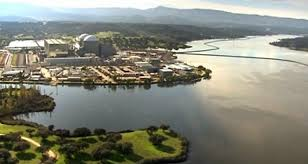
\includegraphics[width=\textwidth]{2Introduction/ArrocampoDam.jpeg}  
    \caption{\label{subfig:Arrocampo_Dam}}
    \end{subfigure}
    \hfill
    \begin{subfigure}[b]{0.45\textwidth}
    \centering
    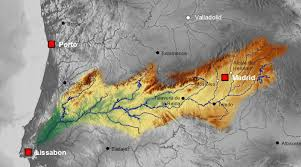
\includegraphics[width=\textwidth]{2Introduction/RioTajo.jpeg}  
    \caption{\label{subfig:TajusRiver}}
    \end{subfigure}
 \caption{a) Arrocampo dam and Almaraz Nuclear Power Plant. b) Tagus river along Spain and Portugal.}
 \label{fig:Arrocampo}
\end{figure}

Each institution of the TRITIUM collaboration is dedicated to the development of a different part of this project:

\begin{enumerate}
\item{} The University of Extremadura group has developed and installed the water purification system to produce water with very low conductivity, $\sigma \approx 10~\mu\text{S}/\cm$ (two orders of magnitude less than raw water, $1000~\mu\text{S}/\cm$). This purification process is very important for two reasons. On the one hand, for maintaining the TRITIUM detector pristine, which is critical for its long-term functionality. On the other hand, to reduce the natural background since several natural radiactive isotopes present in this water (except tritium), such as $\ce{^{40}K}$ and natural radioactive series, are removed. This system is described in section \ref{sec:UltraPureWaterSystem}.

\item{} The French group has developed the passive shielding for the detector. This shielding is made of lead with low intrinsic activity in order to reduce the external natural background of the system. This shielding is presented in section \ref{sec:IntroductionBackground}.

\item{} The Aveiro and Valencia groups have collaborated for designing, developing and building four different prototypes of the TRITIUM detector and active vetos for reducing cosmic events. These prototypes and vetos are described in chapter \ref{chap:Prototypes} and section \ref{subsec:SetUpActiveShield}, respectively. These groups have also carried out simulations of the TRITIUM monitor, which are reported in chapter \ref{chap:Simulations}.

\end{enumerate}

The important characteristics required for the TRITIUM detector are:

\begin{enumerate}

\item{} \textit{Compactness}. This is an important requirement because in the place where the detector is planned to be installed there is little space. Compactness also allows portability and cost reduction.

\item{} \textit{Modularity}. The modularity of the TRITIUM detector is important for flexible geometrical configuration and for improving its tritium detection sensitivity. Modularity also facilitates construction and maintenance.

\item{} \textit{Thin active volume and large active area}. The mean free path of $\beta$ particle from tritium decay is very short. Thus, a thin detector active volume is needed. In practice, an active thickness beyond the mean free path of the tritium electrons only contributes to background. In addition, as reported in section \ref{sec:StateOfTheArt}, the efficiency of this type of detector scales with the active area, so it is crucial to design a detector with the largest possible active area.

\item{} \textit{High detection efficiency for tritium}. As the tritium activities to be measured are very low, the loss of tritium events strongly affects the accuracy of measurements.

\item{} \textit{High specificity to tritium}. The monitor must be able to distinguish tritium signals from other radiactive decays in the sample.

\item{} \textit{Quasi-real time response}. It is crucial that the system operates in quasi-real time ($1~\hour$ or less) in order to detect any anomalous tritium release as fast as possible. 

\item{} \textit{Ruggedness}. The final goal of the project is to install an automatic system working during a number of years requiring only occasional intervention of specialized operators. Therefore, a rugged monitor is required.

\end{enumerate}

In order to measure in quasi-real time, it is needed to work \textit{in situ}, that is, in the same place where the water sample is taken. Working \textit{in situ} has some advantages such as: 1) Cheap running cost, since sampling process, chain of custody, etc. are eliminated. 2) Quasi-real time measurements. 3) Safe monitoring since personal dose is reduced. 4) Changes in activity can be detected quickly.


%In order to get the measurement in quasi-real time it is needed to work \textit{in situ}, that's, in the same place that the sample is taken. Working \textit{in situ} has some benefits:

%\begin{itemize}
%\item{} a faster monitor because we eliminates the process of taking the sample, the chain-of-custody until this sample arrive to this laboratory and the complexity which involve these tasks. 

%\item{} a better monitor since if we can work \textit{in site}, our measurements can be more frequent hence we will can identify cahnges in the activity earlier.

%\item{} a cheaper monitor because we have not only the material costs attached to the sample collection, chain-of-custody of this sample, shipping of this sample to the laboratory, etc. but we have also eliminated the costs attached to the specialized staff who are involving in these tasks. Our detector will only need frequent calibrations each time in order to ensure its correct operation.

%\item{} a safer monitor since the personal exposure dose is reduced and the changes in activity are detected fastly. On top of that we remove the possibles mistakes which can be done by specialized staff.

%\end{itemize} 
	\newpage	
	
\chapter{Design Principles and Components of TRITIUM}\label{chap:DesignPrinciples}
\chaptermark{Design Principles and Components}
	\section{Detector System Overview}\label{sec:MonitorOverview}
	The objective of the TRITIUM project is the design, development, construction and commissioning of an automatic station for real-time monitoring of low levels of tritium in water. To achieve this aim, the TRITIUM group has developed a monitor consisting of several parts, listed below: 

\begin{enumerate}

\item{} The TRITIUM detector, described in chapter \ref{chap:Prototypes}, is based on several modules read in parallel. Each module consists of hundreds of scintillating fibers, section \ref{subsec:PlasticScintillators}, which are in conectact with the water sample measured, read by two coincident photosensors, section \ref{subsec:Photosensors}. The photosensors are photomultiplier tubes (PMT) (section \ref{subsubsec:PMTs}) and silicon photomultipliers (SiPM) (section \ref{subsubsec:SiPM}).

\item{} The ultrapure water system (section \ref{sec:UltraPureWaterSystem}) that prepars the water sample before measurement. This system removes all the organic particles dissolved and all the particles with a diameter greater than $1~\mu\meter$ without affecting the tritium content of the sample. This system is important for two reasons: First, because the mean free path of tritium in water is very short, $5$ or $6~\mu\meter$,  so it is essential to avoid the deposition of particles onto the fibers because this would prevent the tritium decay electrons from reaching the fibers. Second, particles disolved in water may contains raidoactive isotopes like $\ce{^{40}K}$, which whould increase the background. As the water sample has very low tritium counters, to reduce the background is a crucial matter.

\item{} The background rejection system (section \ref{sec:IntroductionBackground}), that has two different parts. The first one is a passive shield (section \ref{subsec:SetUpPassiveShield}), consisting of a lead castle inside of which the TRITIUM detector is located. This castle is employed to eliminate natural radioactive background and cosmic rays with energies of the order of $200~\MeV/$nucleon. The second part is an active veto (section\ref{subsec:SetUpActiveShield}), consisting of two plastic scintillation blocks located inside of a passive shielding, above and below the TRITIUM detector and read by several photosensors. The goal of this active veto is to remove the remaining high energy events ($>200~\mega\eV$) cosmic rays that can travel through the passive shielding and contributo to background. Contrary to low energy cosmics rays, high energy cosmic rays are difficult to be stopped. The technique employed to eliminate their contribution consists of reading the TRITIUM detector in anti-coincidence with the active veto.
%to detect these high energy events and, for each of them, open narrow time windows in which we will not read the Tritium detector to prevent these events from affecting the tritium measurement.

\item{} A monitoring electronic system sends an alarm if the signal limit of the tritium level, $100~\becquerel/\second$, is exceeded.

\end{enumerate}

The different parts of TRITIUM monitor were subjected to tests to verify their correct operation before installing them in the Arrocampo dam. The final goal is to include TRITIUM in the network of automatic stations, REA (section \ref{sec:Introduction}). 
	%\newpage
	
	\section{TRITIUM Detector}\label{sec:TritiumDectectorIntro}
	As discussed in section \ref{sec:StateOfTheArt}, the TRITIUM monitor consists of a chain of three main elements, plastic scintillating fibers, that produce scintillating photons in response to a tritium electron decay, the photosensor, that detects the photons produced in the scintillator and produces an electronic pulse than gives information on the detected photons, and the electronic system, which is in charge of processesing and analyzing the electronic pulse given by the photosensor. A scheme of a scintillation detector setup is shown in Figure \ref{fig:ScintillatorDetector}.

\begin{figure}[hbtp]
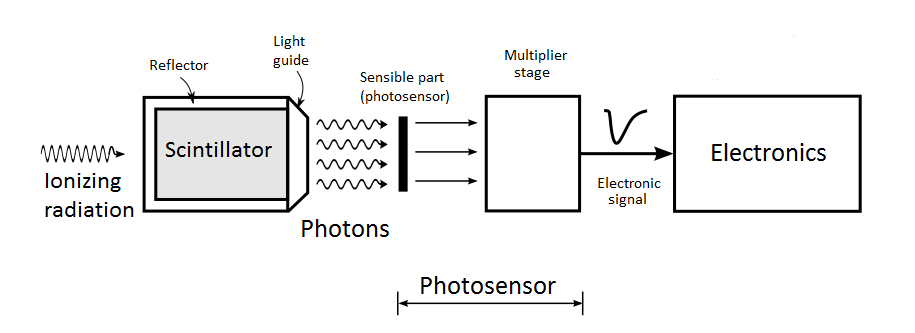
\includegraphics[scale=0.6]{3DesignPrinciples/32Tritium_detector/ScintillatorDetector.png}
\centering
\caption{Scheme of the scintillator detector.\label{fig:ScintillatorDetector}}
\end{figure}
 
	%\newpage
	
		\subsection[Interaction of Particles with Matter]{Interaction of Fast Electrons and Photons with Matter}\label{subsec:Interaction}
		The interaction of particles with matter is described in this section, focusing on the particles and energy range relevant for this thesis, electrons ($0-18~\keV$), photons in the visible range (approx. $380-750~\nm$) and $\gamma$ rays from the background and high energy cosmic rays.

Electrons have a charge, so their interaction with matter is mainly through the orbital atomic  electrons by the Coulomb force. The electron trajectories are much more tortuous than those of heavier particles because of their small mass. Furthermore, electrons lose a significant amount of energy in each collision. The specific energy loss, defined as $S=-\displaystyle{\frac{dE}{dx}}$, gives the energy loss of a particle per unit of path length. In the case of electrons, the total energy loss has two main contributions, the collisions (elastic and inelastic) and the radiative processes (bremsstrahlung) which are roughly proportional \cite{Knoll, Leo},
\begin{equation}
\frac{dE}{dx} \approx \left(\frac{dE}{dx}\right)_{c} + \left(\frac{dE}{dx}\right)_{br} ; \qquad \frac{\displaystyle{\left(\frac{dE}{dx}\right)_{br}}}{\displaystyle{\left(\frac{dE}{dx}\right)_{c}}} \approx \frac{EZ}{700}
\label{eq:ElectronInteraction}
\end{equation}
where $E$ is the energy of the electron in $\MeV$ and $Z$ is the atomic number of the absorbing material. Due to this energy loss, electrons penetrate a material to a depth where they have lost their kinetic energy. This distance, known as the range, is quoted for tritium electrons in Table \ref{tab:MeanFreePathTritium}. 

The material chosen for the detection of tritium decay electrons is organic plastic since, due to its low density, there is a reduced backscattering. It has been chosen in the form of fibres in order to increase the active area and, therefore, the efficiency of the detector.

As photons do not have any charge, their possible interactions with matter are the photoelectric effect, Compton effect, coherent scattering and pair production. The probability of each process, displayed in Figure \ref{fig:ProcessesPhotons}, depends on the energy of the photon, $E_\gamma = h\nu$, and on the atomic number of the material, Z. The optical photons have a wavelength between $400$ and $700~\nano\meter$, that corresponds to energies of the order of the $\eV$. Therefore, pair production does not play any role for optical photons since this requires photon energy of at least $1.022~\MeV$.

\begin{figure}[h]
\centering
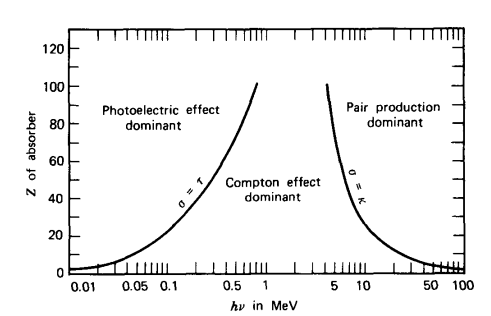
\includegraphics[scale=0.75]{3DesignPrinciples/32Tritium_detector/DominantProcessesPhotons.png}
\caption{Domain regions of the three most probable types of interactions of gamma rays with matter. The lines show the atomic number $Z$ and gamma energy $h\nu$ where two interaction processes are equally likely\label{fig:ProcessesPhotons}~\cite{Knoll}.}
\end{figure}

The photoelectric effect occurs when a photon interacts with an orbital electron in the material, losing all its energy. This energy is absorbed by an electron that is ejected from the atom (ionization). The energy of the resulting electron, $E_e$, is \cite{Knoll, Leo},
\begin{equation}
E_e = E_\gamma - E_b 
\label{eq:PhotoelectricEffect}
\end{equation}
where $E_b$ is the binding energy of the electron in the material. The probability of this effect depends on the number of available electrons in matter through the atomic number $Z$, and the energy of the electron according to the expression \cite{Knoll},
\begin{equation}
\tau \approx \frac{Z^n}{E_\gamma^{3.5}}
\label{eq:PhotoelectricProb}
\end{equation}
Thus, the photoelectric effect is most probable for elements with a high atomic number. This is the reason why these types of elements are the best shields against gamma radiation and why the passive shield of the TRITIUM monitor consists of lead bricks (section \ref{subsec:SetUpPassiveShield}). %This is also the reason why elements with high atomic number like $\ce{Sb}$ ($Z=51$), $\ce{Rb}$ ($Z=37$) or $\ce{Cs}$ ($Z=55$), are used in the cathodes of PMTs. 

The Compton effect occurs when a photon interacts with an orbital electron of the material, transferring part of its energy to the electron which is scattered at an angle $\theta$ with respect to the direction of the incident photon. If the electron binding energy is neglected, the energy transferred to it, $E_e$, is given by \cite{Knoll, Leo},
\begin{equation}
E_e=\frac{\displaystyle{\frac{E_\gamma^2}{m_0c^2}}\left(1-cos\theta\right)}{1+ \displaystyle{\frac{E_\gamma^2}{m_0c^2}}\left(1-cos\theta\right)}
\label{eq:ComptonEffect}
\end{equation}
where $m_0$ is the rest mass of the electron and $c$ is the speed of light in the vacuum. The probability of the Compton effect is proportional to the atomic number $Z$  and decreases with the energy of the photon. As it can be seen in Figure \ref{fig:ProcessesPhotons}, for photon energies in the visible spectrum (of the order of eV), the Compton effect is only likely for very light materials ($Z<4$). For heavier materials the photoelectric effect is dominant.

In the coherent scattering, the atom is neither excited nor ionized and the photon conserves its energy in the collision. Coherent scattering is probable for photons with low energies and materials with high atomic numbers. % and, as it will be shown in section \ref{subsec:PlasticScintillators}, it explains why the produced photons are guided along scintillating fibres. 

Finally, in the pair production process, the photon is converted into an electron and a positron,
\begin{equation}
\gamma \longrightarrow e^- ~ + ~ e^+
\label{eq:pairproductionprocess}
\end{equation}
As can be seen in Figure \ref{fig:ProcessesPhotons}, this is the dominant interaction process for high-energy photons, which are the photons produced by cosmic rays.


%Because of the fact that the energy of the photon doesn't change we will not speak more about this effect but it is important since this effect change de direction of photons and it will affect to their mean free path. 
		%\newpage
					
		\subsection{Plastic Scintillators} \label{subsec:PlasticScintillators}
		Scintillators are widely employed for radiation detection in nuclear physics. Scintillator converts kinetic energy of the incoming particles in to light\footnote{The light is made up of photons in the visible energy range.} which can be detected and quantified. Light emission happens through photon de-excitation of excited atoms.

Light production is linear in a wide energy range of incoming particles. Scintillators should have good optical properties, such as being transparent to the wavelenght of their own emission and having a refractive index as close as possible to that of glass for optimizing optical coupling with photosensors. Photon emission in scintillators is a stadistical process, which means that two identical events will emmit a different number of photons that follows a poisson statistics.

Scintillators can be organic and inorganic. Inorganic scintillators normally have a higher atomic number and density so their light output are higher. Due to these reasons they are better for gamma-ray spectroscopy. Organic scintillators are generally faster and they are commonly used for beta spectroscopy and neutron detection. This section is focussed on organic scintillators since they are the ones used in the TRITIUM project. 

Organic scintillators are based on a scintillator material dissolved in a base solvent, normally aromatic hydrocarbons as $\ce{C_{18}H_{14}}$, $\ce{C_{24}H_{22}N_{2}O}$ or $\ce{C_{15}H_{11}NO}$ with an average atomic numbers of which are between 3,5 and 5.

The scintillator molecules, in which the organic scintillators are based, have a $\pi$-electron structure. The energy levels of their electrons are commonly ilustrated with a Jablonsky diagram, shown in Figure \ref{fig:JablonskyDiagram}, which shows the fundamental singlet state, $S_{0i}$, where the valence electrons are, the excited singlet states, $S_{jk}$, and the excited triplet states, $T_{lm}$. The energy difference between $S_1$ and $S_0$ states is around $3$ or $4~\eV$, in the visible range. As it is shown in the figure, each energy states are splitted in close sublevels separated around $0.15~\eV$. This fine energy structure is due to excitations of molecular vibrational modes tabbed by the second index of the energy states. As the energy levels and sublevels have an energy larger than the termal energy, $0.025~\eV$, non-excited electrons are in the ground state $S_{00}$ at STP\footnote{Standar temperature and pressure conditions}.

\begin{figure}[htbp]
\centering
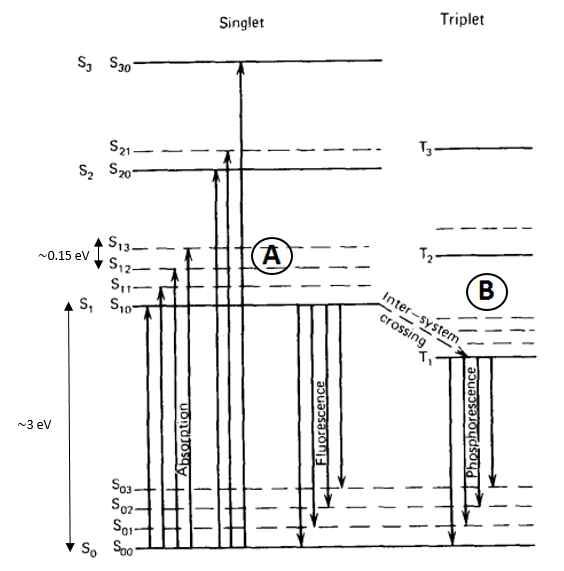
\includegraphics[scale=0.57]{3DesignPrinciples/32Tritium_detector/JablonskyDiagram.png}
\caption{Jablonsky diagram.\label{fig:JablonskyDiagram}~\cite{Knoll}}
\end{figure}

When a particle deposits their kinetic energy in a scintillator, their valence electrons are exited to higher singlet energetic states very fast (times of the order of picoseconds) and are quickly de-excited to the first singlet excited state, $S_{10}$, through non-radiative processes known as internal conversion. These electrons can de-excited to the fundamental single state, $S_{00}$, through three different physical mechanisms:

\begin{itemize}

\item{} Prompt fluorescence(process A in Figure \ref{fig:JablonskyDiagram}), where the electron in the $S_{10}$ energy level  is de-excited to some sublevel of the ground state $S_{0i}$, emitting a photon. This process happens immediately after the excitation of the scintillator molecules (around tens of nanoseconds after excitation). Each scintillator has a characteristic emission spectrum that defines its response due to the fluorescence mechanism. 

Organic scintillators are practically transparent to their own fluorescense emission because there exist a quenching effect in each de-excitation process by which all emmited  photons by the scintillator have less energy than the excitation. This effect is called Stokes shift and it is represented in Figure \ref{fig:StokesShift}.

\begin{figure}[htbp]
\centering
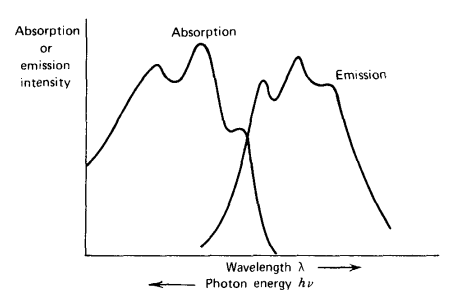
\includegraphics[scale=0.7]{3DesignPrinciples/32Tritium_detector/StokesShift.png}
\caption{Stokes shift.\label{fig:StokesShift}~\cite{Knoll}}
\end{figure}

The intensity of the fluorescence emission in an organic scintillator over time is a combination of two exponential functions, one associated with the lifetime of the level, $\tau$ (on the order of nanoseconds), and the other associated with the energetic level population, $\tau_1$ (on the order of picoseconds) \cite{Knoll}.

\begin{equation}
I=I_0\left(e^{t/\tau} - e^{t/\tau_1}\right) 
\label{eq:IntensityTimeScintillator}
\end{equation}

\item{} Phosphorescence, where the electron that is in the first single excited state cross to a triple excited state (process B in Figure \ref{fig:JablonskyDiagram}) with a process called "intersystem crossing". This is a metastable state with a longer lifetime than phosphorescence. This process happens around $10^{-3}$ seconds after scintillator excitation.

\item{} Delayed fluorescence, which occurs when an electron is in a triple excited state but its transition to the ground state is forbidden. In this case, this electron interacts with another electron in a similar state, falling and return to the first singlet state and quickly de-exciting to the ground state. 

\begin{equation}
T_{1} ~+~ T_{1}~ \longrightarrow ~ S_{1} ~+~ S_{0} ~+~ phonons
\label{eq:DelayFluorescence}
\end{equation}

This emission has the same emission spectrum as immediate fluorescence, but occurs later.
\end{itemize}

As the prompt fluorescence light produces the scintillator signal, detector design should increase it and reduce other possible physical mechanisms. One of the most important parameters is the scintillation yield\footnote{The scintillation yield is a way of expressing the efficiency of the scintillator in converting the energy deposited by the particle into photons.}, defined as the the number of photons emitted by unit of absorbed energy. This yield depends on the type of particle and on other mechanisms that doesn't produce prompt fluorescence, like phosphorescence or delayed fluorescence or even internal conversion. The scintillator yield is normally quoted by the manufacturer for mips\footnote{The MIP, Minimum Ionized Particles, is a particle that has the speed that generate minimum ionization, that's, for example, electrons with $500~\keV$ or more}.

		%\newpage
		
			%\subsubsection{Plastic scintillation fibres}\label{subsubsec:PlasticScintillatorFibres}
			Plastic scintillators are organic scintillators that has been disolved in a solven and polimerized. They are easy to machine and can take any desired shape during construction. Among the forms most used today we can find blocks, thin sheets, cylinders, etc.

In our experiment we have been working with an plastic scintillator in the form of fiber, specifically, commercial fibers BCF-12 from Saint-Gobain Crystals Inc \cite{DataSheetBCF12Fiber}. This type of fiber was chosen as the result of a comparative study \cite{TFGAlberto} among some of the best-known commercial manufacturers, such as Kuraray \cite{DataSheetKuraray}. 

The BCF-12 fibers consist of a scintillated core, whose material is polystyrene, one of the most used solvents for plastic scintillators \cite{Knoll}, with the posibility of surounding it of a cladding of polymethylmethacrylate (PMMA) (smaller refractive index than core in order to archieve a critical angle) or a multicladding (second cladding) with even smaller refractive index.

When a particle deposits all or part of its kinetic energy, some photons are produced in the fiber core as a result of the scintillating process. The number of photons produced depend on the scintillation efficiency, whose value is around $2.4\%$ for the fibers used (BCF-12), which means that $8000$ photons will be produced per $\MeV$ for a mip\footnote{The mip, minimum ionizing particle, is a particle that has the speed that generate minimum ionization.} (scintillation yield). For instance, for tritium electron, this fibers will release a maximum of around 148 photons (when tritium electron has the maximum energy, $18.6~\keV$), probably less because electrons with these energies are not mips.

These photons will shape the useful part of the response of the scintillator (fluorescence) for us. The energy (or wavelength) of these scintillated photons follows the distribution of their emission spectrum which, for the used fibers, is shown in Figure \ref{fig:EmissionSpectrumFibers}.

\begin{figure}[htbp]
\centering
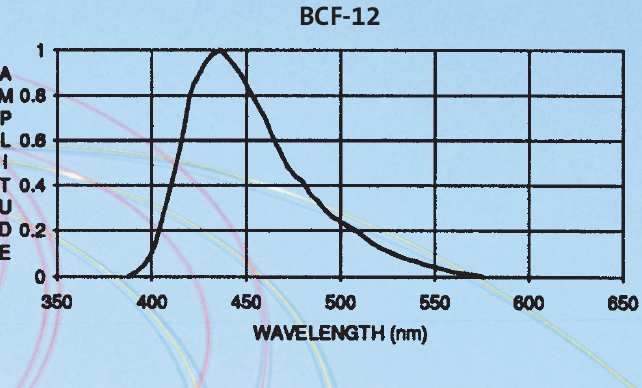
\includegraphics[scale=0.5]{3DesignPrinciples/32Tritium_detector/EmisionBCF12.png}
\caption{Emission spectrum of BCF-12 fibers of Saint-Gobain.\label{fig:EmissionSpectrumFibers}~\cite{DataSheetBCF12Fiber}}
\end{figure}

After the production of scintillated photons, we need to guide these photons to the sensitive part of the photosensor where we will detect them with some probability. Fibers (and scintillators in general) use the optical property of Snell's law \cite{Snell} to guide their photons to the desired part (the ends of the fibers). It is based on the interface created between the core and the surrounding material. When a photon hits this interface, it is refracted (and therefore lost) following the Snell equation, \ref{eq:Snell}. If the surrounding material has a lower refractive index than the core of the fiber, there exist a critical angle, $\theta_c$, at which, for angles equal or larger than this one, the photons will be totally reflected (and therefore conserved in the fiber for being guided). This effect is showed in Figure \ref{fig:Fiber_physic}.

\begin{equation}
n_0~sen(\theta_0) = n_1~sen(\theta_1) \longrightarrow \theta_c = asen\left(\frac{n_1}{n_0} \right)
\label{eq:Snell}
\end{equation}

There exist a parameter which define the efficiency of the scintillator to guide photons, the trapping efficiency or photon collection efficiency. For BCF-12 fibers with optical clad is between $3.44\%$ and $7\%$ (depending if the event was detected near the fiber axis (minimum) or near the core-clad interface(maximum)) and for no clad fibers BCF-12, it is a bit larger but presents some problems as we will see.

Therefore, from these $148$ photons initially created with the tritium electron with the maximum energy, only a maximum of around 10 photons (for maximum trapping efficiency) will arrive to our photosensor. As you can see, we work with very weak detector signals, where there is more electronic noise and, as you will see in future chapters, we have made a big effort to reduce this electronic noise as much as possible with several technics.

In Figure \ref{fig:Fiber_physic} we can see how a scintilalting fiber works.

\begin{figure}[htbp]
\centering
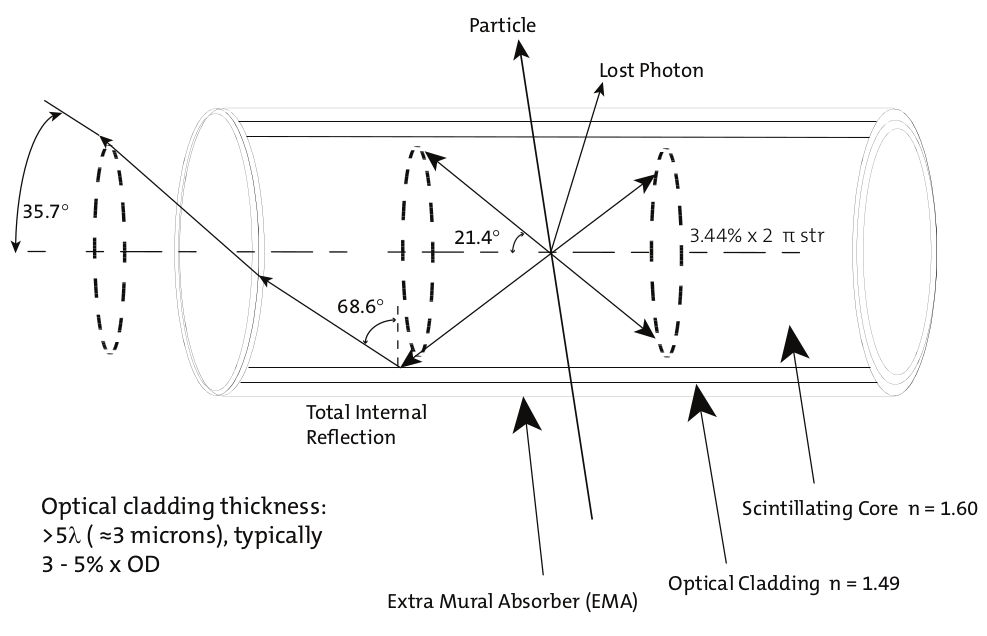
\includegraphics[scale=0.5]{3DesignPrinciples/32Tritium_detector/Fiber_data_sheet.png}
\caption{How photons are collected in a fiber with single clad.\label{fig:Fiber_physic}~\cite{DataSheetBCF12Fiber}}
\end{figure}

The cladding material is useful for protecting the core surface from dirt or aggressive external agents that can reduce the light collection but at the cost of losing some light because it increase the critical angle. In Table \ref{tab:CriticalAngles} we have three different examples where this effect is ilustrated.

\begin{table}[htbp]
%%\centering
\begin{center}
\begin{tabular}{|c|c|c|}
\hline
Material & Refractive index & critical angle ($\degree$) \\
\hline \hline \hline
Air & 1 & $42.98$ \\ \hline
Water & 1.33 & $62.47$ \\ \hline
Cladding of PMMA & 1.49 & $76.26$ \\ \hline
\end{tabular}
\caption{Critical angles asociated to different interfaces created with polystyrene, $n_0=1.6$, and other materials}
\label{tab:CriticalAngles}
\end{center}
\end{table}

This is what theoretically happens but, in the practice, it's difficult to archieve a perfect air-core or water-core interface and it will affect to the light collection. Due to the reason that the commercial claddings are thicker ($30~\micro \meter$) than the mean free path of tritium in water ( around $5~\micro\meter$) we cannot use commercial cladding in our detector hence we will need to take special attencion for archieving a water-core interface enough good. To overcome this problem, as we will see in section \ref{subsubsec:CleaningProcess}, we have used a special protocol developed in the ICMOL laboratories for preparing fibers before we use them for tritium detection.

Some of the most important parameters that descript a scintillator are summarized in Table \ref{tab:ParametersFibersBCF12} for the fibers used.

\begin{table}[htbp]
%%\centering
\begin{center}
\begin{tabular}{|c|c|c|}
%\hline
%Material & Refractive index \\
\hline \hline 
Core material & Polystyrene \\ \hline
Core refractive index & 1.60 \\ \hline
Density ($\gram/\cm^3$) & 1.05 \\ \hline
Cladding material & Acrylic (PMMA) \\ \hline
Cladding refractive index & 1.49 \\ \hline
Cladding thickness ($\mu\meter$) & 30 \\ \hline
Numerical aperture & 0.58 \\ \hline
Trapping efficiency & 3.44\% minimum \\ \hline
No. of H atoms per cc (core) & $4.82 \cdot{} 10^{22}$ \\ \hline
No. of C atoms per cc (core) & $4.85 \cdot{} 10^{22}$ \\ \hline
No. of electrons per cc (core) & $3.4 \cdot{} 10^{23}$ \\ \hline
Radiation lenght (cm) & 42 \\ \hline
Emission peak (nm) & 435 (Blue) \\ \hline
Decay Time, (ns) & 3.2 \\ \hline
1/e Length (m) & 2.7 \\ \hline
Scintillator yield (\#$\gamma$/MeV) & $\sim 8000$ \\ \hline
Operating Temperature & $-20\degree C$ to $50\degree C$ \\ \hline
\end{tabular}
\caption{Properties of BCF-12 fibers from Saint-Gobain Inc. \cite{DataSheetBCF12Fiber}}
\label{tab:ParametersFibersBCF12}
\end{center}
\end{table}

%Bunch -> manojo de fibras

%bundle -> haz de fibras%
			%\newpage
			
		\subsection{Light Detection in Photosensors}\label{subsec:Photosensors}
		The scintillating photons created in the core of the fiber and guided to its ends are detected by photosensors. Photosensors have a sensitive part that is optimized to detect photons in a range of energy (usually in the visible range) with a certain probability, called quantum efficiency. The photosensors produce an electronic signal that carries information about the detected photons such as their number, detection time, etc. There are many available photosensors that rely on various physical processes, such as photomultiplier tubes (PMTs), silicon photomultipliers (SiPM) or Charge-Coupled Devices (CCD).  %Each one of these will have different properties and it has to be chosen the one which fit better for the objective of the experiment.

The optimization of the efficiency of a scintillation detector is essential. To do so, the emission spectrum of the scintillator (Figure \ref{fig:EmissionSpectrumFibers} for the fibers used) must overlap as much as possible with the detection efficiency spectrum of the photosensor chosen. The detection efficiency spectrum of a photosensor gives the probability of detecting photons as a function of wavelength. The efficiency of a detector is proportional to the product of both, the emission and the detection efficiency spectra, and this is largest when both spectra match.

The requirements imposed on the photosensor of the TRITIUM detector are that they be very fast, have high gain and are able to detect a single photon with high photodetection efficiency. Two different porposals for the TRITIUM detector are investigated, SiPMs and PMTs. Both meet these requeriments since they are very fast (of the order of $\nano\second$), have high gain (of the order of $10^{6}$) and have a high photodetection efficiency (around $50\%$ for SiPMs and $30\%$ for PMTs). Each porposal has their own advantage. SiPMs are more robust and need a lower supply voltage (of the order of $50~\volt$) than PMTs (of the order of $1000~\volt$). Furthermore, due to this different in the supply voltage, SiPMs has a smaller cost per unit of channel than PMTs since a SiPM array, which can be feed with a single channel. However PMTs, which are the conventional choice, have lower dark count rate than SiPM a much lower dependence with the temperature.



%A certain portion (in an optimal case nearly 100\%) of the scintillation photons reach the light detector, which has to be sensitive enough to detect a small number of photons. The detector then produces a signal pulse, which has a height proportional to the number of photons hitting the detector. The signal pulse of the detector is processed by the electronics, and as a result a pulse height spectrum is produced (see Section 3.5).

%This spectrum corresponds to the energy spectrum of the detected particles.

		%\newpage
	
			\subsubsection{Photomultiplier Tubes (PMTs)}\label{subsubsec:PMTs}
			Photoelectron multiplier tube, PMT, has been employed as photosensors in nuclear physics during decades. They detect the scintillating photons that reach its sensitive part, the photocathode, and produce an electronic signal, large enough to be easily measured. In Figure \ref{fig:SchemePMT} a schematic drawing of a PMT is given. This consists of a vacuum tube that has a glass window through which photons can penetrate. The electrons created in the photocathode travel in vacuum. 

\begin{figure}[htbp]
\centering
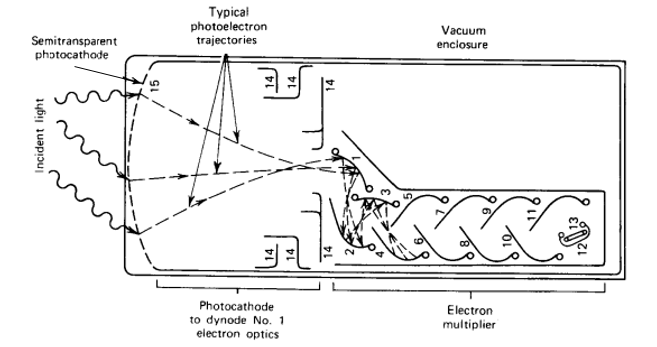
\includegraphics[scale=0.6]{3DesignPrinciples/32Tritium_detector/PMTschematic.png}
\caption{Scheme of a PMT.\label{fig:SchemePMT}~\cite{Knoll}}
\end{figure}

The signal production has two phases:
\begin{enumerate}
\item{} In the photocathode, photons are converted in photoelectrons through photoelectric effect. The photocathode consists of a thin layer, of the order of nanometers, deposited on the inner surface of the PMT window. The material of the photocathode is chosen to optimize the probability of producing photoelectric effect with the scintillating photons. The PMTs used in TRITIUM experiment are the model R8520-406 from Hammatsu \cite{DataSheetPMTs} and the material of their photocathode is Bialkali\footnote{The bialkali material is based on the elements $\ce{^{121}_{51}Sb}$, $\ce{^{85}_{37}Rb}$ and $\ce{^{132}_{55}Cs}$}.

The response of the PMT at long wavelengths is limited mainly because photon energy is not enough to produce a photoelectric effect or the emitted photoelectron does not have enough energy to overcome the material-work function. The response of the PMT at short wavelengths is limited due to absorption in the window material, quartz in our case. Thus, the response of the PMT has a strong dependence on the energy of the photon. The quantum efficiency (QE)  spectrum, shown in Figure \ref{fig:QuantumEfficiencyPMT} for the PMT used in TRITIUM, is defined as the ratio of the number of photoelectrons produced at the cathode of the PMT and the number of photons reaching it.

\begin{figure}[htbp]
\centering
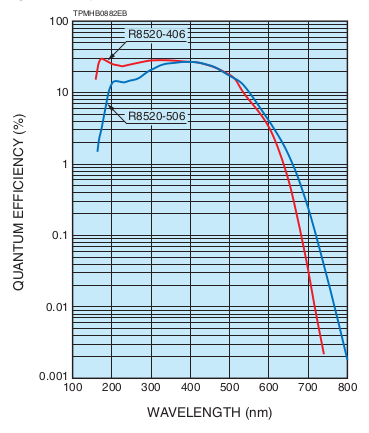
\includegraphics[scale=0.5]{3DesignPrinciples/32Tritium_detector/QuantumEfficiencyPMT.png}
\caption{Quantum efficiency spectrum for the PMT used (R8520-406).\label{fig:QuantumEfficiencyPMT}~\cite{DataSheetPMTs}}
\end{figure}

The maximum values of the PMT quantum efficiency is usually between $20\%$ and $30\%$ \cite{Knoll} (a little bit less than $30\%$ for the PMTs employed). The emission spectrum of the scintillating fibers used, Figure \ref{fig:EmissionSpectrumFibers}, matches the quantum efficiency spectrum of the PMTs used, Figure \ref{fig:QuantumEfficiencyPMT} and the position of both peaks is very close, $435~\nm$ and $420~\nm$ for fibers and PMT respectively.

\item{} As the number of photoelectrons produced in the photocatode is very small, an electron multiplication stage is employed to obtain an electronic signal of sufficient size to be processed by the electronic system. The amplification stage is based on three elements, focusing electrodes, dynodes and anode, which are metallic plates with a shape and position designed to optimize the collection and multiplication of electrons. A high voltage (HV) is applied to the PMT which is distributed between all this elements, including the photocathode, with the help of electronic circuit. A positive HV, grounded in the photocathode, is interesting for measuring PMT currents, and a negative HV, grounded in the anode, gives a faster response. The comercial electronic circuits of Hammatsu are shown in Figure \ref{fig:VoltageDividerCircuit}.

\begin{figure}[h]
\centering
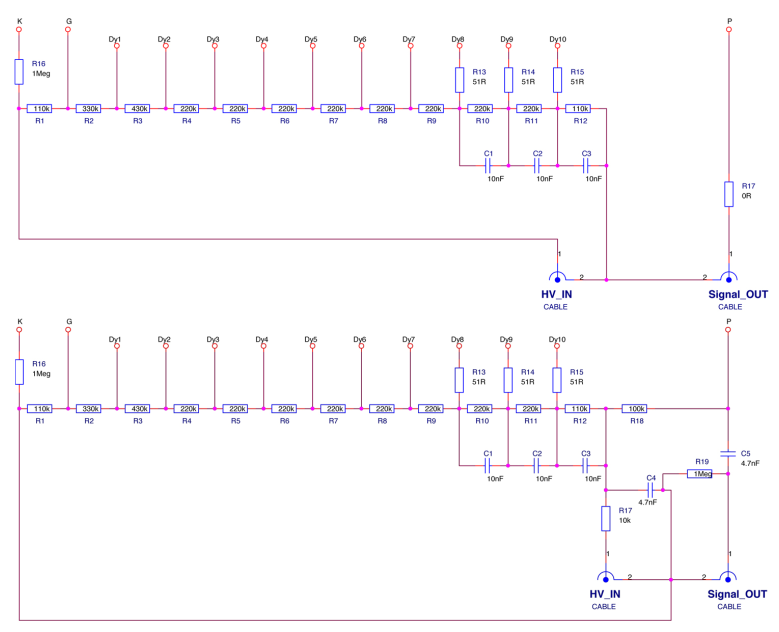
\includegraphics[scale=0.5]{3DesignPrinciples/32Tritium_detector/VoltageDividerPMT.png}
\caption{Hamamatsu commercial voltage divider electronic circuit. Upper circuit with negative supply and lower circuit with positive supply.\label{fig:VoltageDividerCircuit}~\cite{DataSheetPMTs}}
\end{figure}

%The electronic circuit that can be supplied with negative voltage is faster due to the ausence of the capacitances C4 and C5, but the other circuit, supplied with positive voltage, can be interesting for other tasks like the measurement of PMT currents. We will use both, depends on the objective of the study.

Focusing electrodes guide the photoelectrons to the first dinode. They have a collection efficiency (CE) defined as the ratio of the number of photoelectrons reaching the first dinode and the number of photoelectrons leaving the photocathode and its value is around $80\%$. The dynodes achieve the electron multiplication. A voltage difference between adjacent dynodes accelerates the electrons and produce their multiplication. The multiplication factor of each dynode, $\delta$, is commonly around 5 and is strongly dependent on the HV. If all dynodes have the same gain, the overall gain of a PMT with N dynodes is \cite{Knoll}:
\begin{equation}
G = CE\cdot{} \delta^N
\label{eq:PMTGain}
\end{equation}
that give an overall gain of a PMT of the order of $10^6$, strongly dependent on the applied HV.

The multiplication stage adds an uncertainty in the measurement. Working without gain allows to count the number of photons that reach the PMT. This can be done by short-circuiting all the dynodes and the anode and collecting the signal directly of the photocatode. This special setup was used for fiber characterization, described in section \ref{subsec:CharacterizationFibers}.

\end{enumerate}

The output pulse of a PMT has a width of the order of tens of nanoseconds. The multiplication process can be described as a Poisson statistical process. For each electron in the first dynode, G new electrons are created with a variance of $\sqrt{G}$.

The output signal of a PMT is linear with the number of photons that reach its sensitive part up to a saturation limit, at which the linearity is lost. This limit depends on the PMT model.

The photocathode may emit electrons without any scintillation light. This signal, called dark current, $I_{DC}$, can  arise due to thermoionic emission. For the PMTs used, this value is around $2~\nano\ampere$ according to their data sheet.

The characterization of the PMTs used for dark current, gain for several HV and quantum efficiency,  was done at IFIC in the framework of NEXT experiment \cite{CalibrationPMTsNEXT}. 
			%\newpageand
		
			\subsubsection{Silicon Photomultiplier Array}\label{subsubsec:SiPM}
			The Silicon Photomultiplier (SiPM) are a bind of photosensor, based on semiconductor materials, developed in recent years. They are replacing progresively conventional PMTs in many experiments and applications. They archieve outstading photon-counting capabilities with high gain and high photodetection efficiency comparing to PMT. They have conveninent characteristics as insensitiveness to magnetic fields, low operating voltage and compactness.

SiPM are based on p-n junctions, made with special techniques to archieve a good contact between both surfaces.

The voltage at which the SiPM changes from proportional to geiger mode is called the breakdown voltage, $ V_ {BR} $. At a lower voltage it works in proportional mode but at a higher voltage, it switch to Geiger mode. The measurement of the breakdown voltage is one of the most important parametes to characterize the SiPM and Its determinations is described in section \ref{sec:CharacterizationSiPM}.

The SiPM, formed by a matrix of APDs which are photodiodes operating in Geiger mode. A scheme of an APD is shown in Figure \ref{fig:SchemeAPD}. It has p+ and a n+ layers. 

\begin{figure}[htbp]
\centering
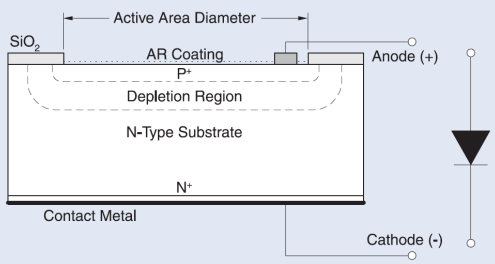
\includegraphics[scale=0.6]{3DesignPrinciples/32Tritium_detector/APD_scheme.png}
\caption{Scheme of a APD and electrical symbol used.\label{fig:SchemeAPD}~\cite{OSI}}
\end{figure}
 
These APDs, called pixels when they are part of a SiPM, are connected in parallel and the sum of all of them is read. The output signal of the pixels are quite similar regardless of the energy deposited, with some difference because of the uncertainty due to the SiPM manufacturing process and the statistical nature of the detection process. The energy deposited in each APD is not known but, as all SiPM pixels are read at the same time, the charge of the output signal when n photons are simultaneously detected is n times the charge of a sigle photon, as can be seen in Figure \ref{fig:PulsesOfSiPM}. Due to this property, after a correct calibration of SiPMs the number of detected photons we have detected is linearly related to the output signal. 

As the number of scintillating photons is proportional to the deposited energy, the linearity of its output signal and the deposited energy is obtained.

\begin{figure}[htbp]
\centering
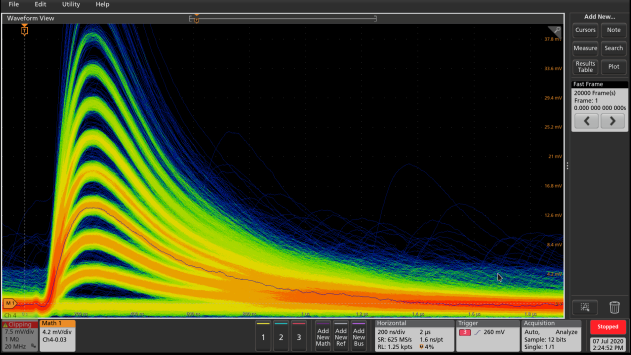
\includegraphics[scale=0.6]{3DesignPrinciples/32Tritium_detector/Several_SiPM_pulses.png}
\caption{Using persistence on the oscilloscope to show several pulses with different heights. Each height associated with a different number of  SiPM pixels lit at the same time.\label{fig:PulsesOfSiPM}}
\end{figure}

On top of that, these pixels need to be so small\footnote{Pixel sizes for commercial SiPMs are $50$ or $75\mu\meter$ \cite{DataSheetHammamatsu_1_SiPM_50}, \cite{DataSheetHammamatsu_1_SiPM_75}} that, if the photon density to be detected is low enough, we only detect one photon in each pixel. If it doesn't happen, we will detect two or more photons with the same pixel but the output signal will be the same as one detected photon, so we will have a loss of linearity of our output signal. This effect is known as saturation and it is important to know the photon density at which it happens for our SiPMs. The experimental measurements of this effect, which have been done for our SiPMs, is shown in section \ref{sec:CharacterizationSiPM}. SI LA MIDO YO PERFECTO, SI NO DECIR QUE PARA NEUSTRO CASO NO ES IMPORTANTE PORQEU ESTAMOS MIDIENDO MUY POCOS FOTONES POR EVENTO.

Each of these pixels has a quenching resistance\footnote{The tipical valuer of this quenching resistance for commercial SiPMs is around $500~\kilo\Omega$} in series that is used to stop the current produced when this pixel has detected a particle. It is used for limit the current drawn by the diode during breakdown and reduce the reverse voltage seen by the diode to one below the breakdown voltage. After that, the voltage seen by the diode is reset to the bias voltage and this pixel is ready to detect a new particle again. In Figure \ref{fig:ChenchingResistance} (left) a diagram of these chenching resistances and APDs in a SiPM and (right) how it works is shown respectively.

\begin{figure}[htbp]
\centering
{
%\subfloat[PDE]
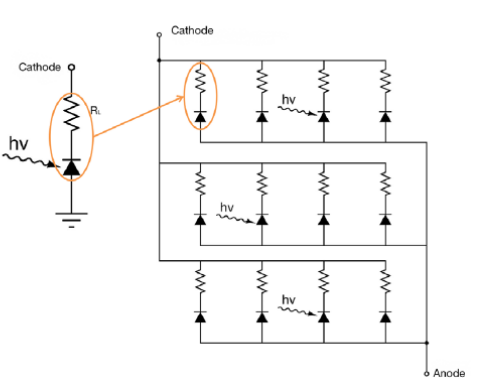
\includegraphics[scale=0.35]{3DesignPrinciples/32Tritium_detector/Quenching_resistence_of_a_SiPM_scheme.png}
%\caption{Simple electronic model of a SiPM.\label{fig:ElectricModelSiPM}~\cite{DataSheetSensL}}
}
{
%\subfloat[Espectro de emisión]
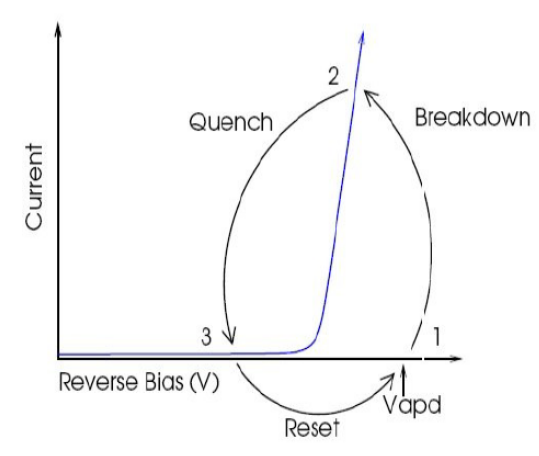
\includegraphics[scale=0.5]{3DesignPrinciples/32Tritium_detector/How_a_quenching_resistence_in_a_SiPM_works.png}
%\caption{Output current of a SiPM as a function of the reverse voltage. It show that the quenching mechanism is essential for working with SiPMs\label{fig:HowSiPMworks}~\cite{DataSheetSensL}}
}
\caption{(Left) Electronic scheme of a SiPM and (right) output current of a SiPM as a function of the reverse voltage. It show that the quenching mechanism is essential for working with SiPMs\label{fig:ChenchingResistance}~\cite{DataSheetSensL}}
\end{figure}

In this simple electrical scheme we can see that all pixels have a common cathode and anode which means that, as we said before, they are at the same bias voltage and the output is the sum of all of them.

We have a lot of names to refer to these photosensors such as SiPMs, MPPCs, G-APDs, SSPMs, MRS-ADPs or AMPDs. The candidate for TRITIUM project is S13360-6075 from Hamamatsu photonics \cite{DataSheetHammamatsu_1_SiPM_75} because its characteristics are the ones that best fit our objectives since this model has super low afterpulses, crosstalk and dark counts than other SiPM models from Hamamatsu. Its characteristics and properties are shown in Table \ref{tab:PropertiesOfSiPM75}. 

\begin{table}[htbp]
%%\centering.
\begin{center}
\begin{tabular}{|c|c|}
\hline
Parameter & Numerical value \\
\hline \hline \hline
Serie & $S13360$ \\ \hline
Model & $6075$ \\ \hline
Pixel Pitch ($\mu\meter$) & $75$ \\ \hline
Effective photosensitive area ($\mm^2$) & $6.0 \times 6.0$ \\ \hline
Number of pixels & $6400$ \\ \hline
Fill factor & $82\%$ \\ \hline
Refractive index of windows material & $1.55$ \\ \hline
Operating temperature range ($\degree C$)& $[-20,60]$ \\ \hline
Spectral response range, $\lambda$ ($\nano\meter$) & $[320, 900]$ \\ \hline
Peak sensitivity wavelength, $\lambda_p$ ($\nano\meter$) & $450$ \\ \hline
PhotoDetection Efficiency, PDE, $\lambda=\lambda_p$ ($\%$) & $50$ \\ \hline
Dark counts, Typical/Maximum (kcps) & $2000/6000$ \\ \hline
Terminal capacitance, $C_t$ ($\pico\farad$) & $1280$ \\ \hline
Gain, M, & $4 \cdot{} 10^6$ \\ \hline
Breakdown Voltage, $V_{BR}$ ($\volt$) & $53$ \\ \hline
Cross talk probability($\%$) & $7$ \\ \hline
Temperature coefficient $\Delta TV_{op}$ (m$\volt/\degree C$) & $54$ \\ \hline
\end{tabular}
\caption{Characteristics of SiPM S13360-6075 from Hamamatsu Photonics \cite{DataSheetHammamatsu_1_SiPM_75}.}
\label{tab:PropertiesOfSiPM75}
\end{center}
\end{table}

These characteristics and properties will be explained and their experimental measurements will be shown in section \ref{sec:CharacterizationSiPM}. These numerical values, which appear in Table \ref{tab:PropertiesOfSiPM75}, are provided by Hamamatsu photonics but it is only an approximation for this model. These parameters must be determined experimentally for each SiPM used because it can be very different even if it is the same model.

It must be taken into account that we will do this characterization at the level of a single SiPM because, at the beginning, it is easier to understand the results but we will work with a matrix of them and we will have to do this characterization for each matrix used. 

The matrices under consideration are the model "S13361-6050" from Hamamatsu, which consists of a $4\times 4$ SiPM matrix where the active area of each SiPM is $6\times 6~\mm$ \cite{DataSheetHammamatsu_array_SiPM_6050} or the model "S13361-3050" from Hamamatsu, which consists of a $8\times 8$ SiPM where the active area of each is $3\times 3~\mm$ \cite{DataSheetHammamatsu_array_SiPM_3050}. They are a commercial matrices from Hamamatsu and, as you can see, the total active area that we will cover with these arrangements is the same in both cases, $24\times 24~\mm$ and it is approximatelly the same that the active area covered with the PMTs used, which has been shown in the previous section.

These matrices have a common bias voltage and common ground for all SiPMs that are contained and we will have an output signal for each SiPM. 

We hope to obtain better results with the 4x4 matrix for theoretical reasons which we will see in section \ref{sec:CharacterizationSiPM} like larger PDE, mainly due to a larger active area but it is something that we will have to verify with experimental measurements.




Nuestro SiPM esta dopado? con que?
			%\newpage
			
			\subsubsection{Photosensors of TRITIUM}\label{subsubsec:ComparisonPhotosensors}
			Two different types of photosensors are proposed for the TRITIUM monitor, PMTs and SiPM arrays. Each type of photosensor has advantages and disadvantages and must be experimentally tested to ensure the most suitable option. PMTs are used in the TRITIUM prototypes developed by the Aveiro experimental group while SiPM arrays are used in the TRITIUM prototypes developed at IFIC.

%PMTs with and without gain have also been used in Valencia to perform various laboratory measurements such as R\&D studies with fibers, characterization of the active veto and test measurements of the TRITIUM prototypes developed.

The IFIC group has chosen the SiPM matrix option for the photosensor option for its advantages over PMTs, which are compactness and robustness, necessary to work during several years without supervision, larger efficiency for detection of photons in the visible range and more economical price, both the photosensor and the electronic. % sytem necessary to feed them and process and analyze their output signal. However, the SiPM arrays have a higher dark count rate compared to the PMTs, which is a relevant disadvantage for the purpose of TRITIUM monitor since low activities of tritium are intended to be measured.
			%\newpage
					
		\subsection{Electronics}\label{subsec:IntroductionElectronicalSystem}
			The electronic system is in charge of reading, processing and analyzing the output signal of photosensors and providing output information about tritium detection. This electronic system depends on the type of output information that is desired and on the detector configuration used.

%In each type of detector configuration, this electronic system will also be different depending on the type of information we want to obtain. For example, it will be different if we want to obtain an energy spectrum as output information or simply a number such as the number of counts per second of our detector or the output electrical current. Each electron system that has been used in our experiment will be explained during this section.

 
			%\newpage
	
			\subsubsection[Electronic for PMTs]{Electronics for PMTs}\label{subsubsec:PMTsElectronicalSystem}
			PMTs were used in TRITIUM experiment for two main objectives. On the one hand, to determine the amount of incident photons that reach the PMT photocathode, which is important to characterize fibers, and, on the other hand, to measure the energy of events, which allows us to discriminate events according to their origin, obtaining an energy spectrum of tritium events in water from laboratory prototypes.

To know the amount of photons that reach the photocathode, as explained above, the PMT should work without internal gain since it introduces a large uncertainty in the measurement. For that end, the homemade electron multiplication stage of Figure \ref{fig:ElectronicSchemeBasePMTNoGain} is employed. 

As the electrons are not multiplied, the output pulse of the photosensor is very small (currents of the order of tens of nanoamperes) and a special readout system is needed. The chosen system is Keithley 6487 Picoammeter/Voltage Source \cite{DataSheetKeithley6487}, a commercial system from Keithley. This system has some useful options such as automatic baseline correction, the ability to read currents of the order of picoamperes and the possibility of carrying out mathematical operation on the signal, such as the average of N measurements with the associated statistical error, where N is programmable by the user ($N=100$ in all our studies). 

To determine the energy of the events, the gain of the PMT has to be restored by removing the short-circuit of the electron multiplication stage. The number of PMTs used simultaneously was one, two or four, depending on the setup. A simplified scheme of the electronic chain employed in each case is shown in Figures \ref{subfig:ElectronicConfiguraiton1PMT}, \ref{subfig:ElectronicConfiguraiton2PMT} and \ref{subfig:ElectronicConfiguraiton4PMT}, based on various NIM modules\footnote{The Nuclear Instrumentation Module (NIM) is a standard specification convention for electrical and mechanical parameters defined in electronic modules used in experimental nuclear and particle physics.}.

\begin{figure}
\centering
    \begin{subfigure}[b]{1.0\textwidth}
    \centering
    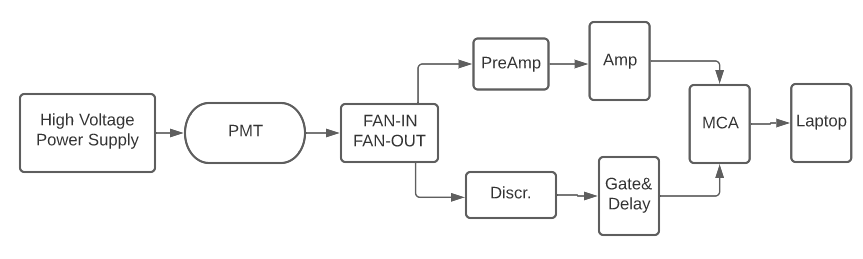
\includegraphics[width=\textwidth]{3DesignPrinciples/32Tritium_detector/Electronical_Scheme_1_PMT.png}  
    \caption{\label{subfig:ElectronicConfiguraiton1PMT}}
    \end{subfigure}
    \hfill
    \begin{subfigure}[b]{1.0\textwidth}
    \centering
    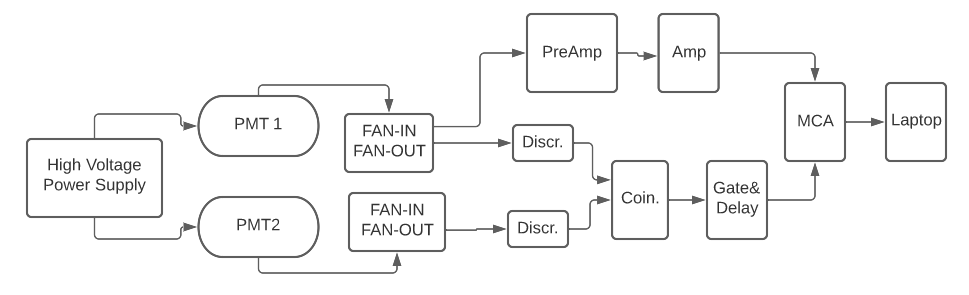
\includegraphics[width=\textwidth]{3DesignPrinciples/32Tritium_detector/Electronical_Scheme_2_PMTs.png}  
    \caption{\label{subfig:ElectronicConfiguraiton2PMT}}
    \end{subfigure}
    \hfill
    \begin{subfigure}[b]{1.0\textwidth}
    \centering
    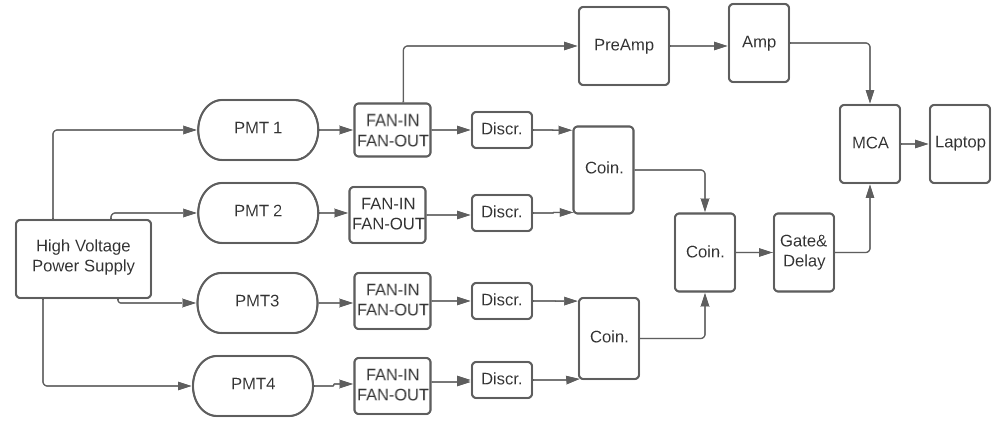
\includegraphics[width=\textwidth]{3DesignPrinciples/32Tritium_detector/Electronical_Scheme_4_PMTs.png}  
    \caption{\label{subfig:ElectronicConfiguraiton4PMT}}
    \end{subfigure}
 \caption{Schemes of the different electronic for measuring with PMTs. a) Employed when only one PMT is used. b) Employed when two PMTs are used in time coincidence. c) Employed when four PMTs are used in time coincidence.}
 \label{fig:ElectronicConfiguraitonsPMT}
\end{figure}

The PMTs were biased in all the cases by TC 952 High Voltage Supply from Tennelec \cite{DataSheetHVSupplyTennelec}, which has four channels. If two or more configurations are needed, a second voltage supply HV Power Supply N 1130-4 from Wenzel Elektronik company \cite{DataSheetHVSupplyWenzel} with 4 additional channels, was employed. As it can be seen in the figures, there are two different lines followed by the PMT output signals, the amplification line, used to create an energy spectrum, and the time coincidence line, used to make time coincidences. Therefore, an analogic FAN IN-OUT module was used to duplicate the input signal. The module employed was the Quad linear FAN IN-OUT MODEL 740 from Philips Scintific \cite{DataSheetFANINOUT}, which has four channels. One output signal was used as the input for the amplification part and the second output was used as input for the time coincidence electronics.

\begin{enumerate}

\item{} The amplification line, which is the same for the three configurations, provides the energy information and is based on two steps;

%We have to take into accout that we have only used the signal from one PMT for the amplification part. We could have added a stage where we add the four PMT output signals and it would probably improve our results, but since our ultimate goal is to work with SiPM, we have not delved into that.

%The electronic path we have followed to achieve this amplification is:

\begin{enumerate}

\item{} The output signal is integrated by a preamplifier, which gives an output signal with a heigth proportional to the charge of the input pulse. This signal has a long tail\footnote{The length of the tail is, $\tau=RC$, where R is the input resistance and C is the capacitance used. It is the typical output signal in RC circuits.} produced by the preamplifier capacitance. The preamplifier used was "MODEL 9326 FAST PREAMP" from ORTEC \cite{DataSheetPreAmp}.

\item{} The output signal from the preamplifier is lead to the amplifier which gives a gaussian shaped output signal. The amplifier modules were 575A and 671 from ORTEC \cite{DataSheet575Amp, DataSheet671Amp}. An example of the output signal for 575A module is shown in Figure \ref{fig:InputSignalsMCA}, green color.

\end{enumerate}

\item{} The time coincidence line contains the time information and gives the gate that triggers coincident signals of both PMTs. This line consists of the following branches,

\begin{enumerate}

\item{} The output signal of the FAN IN-OUT module of each PMT is introduced into a discriminator module that gives a logic signal of $-1.2~\volt$ height and of $240~\nano\second$ width when a given threshold is exceeded. The discriminators employed are  Octuple Constant-Fraction Discriminator CF8000 module from ORTEC \cite{DataSheetDiscriminator} and 4 channels discriminator model 84 from CAEN \cite{DataSheetDiscriminatorCAEN}.

\item{} Time coincidences are required to ensure that detected events come from the scintillating fibers and to remove external light and dark current. The two logic signals given by the discriminator from the two PMTs that read a detector are introduced in a coincidence module which generates an output signal of $-1.4~\volt$ heigh and of $20~\ns$ width, when both imputs are in time coincidence. The modules used were Coincidence Unit Model 465 from LeCroy \cite{DataSheetCoincidenceLeCroy} and Coincidence Type N6234 from CERN-NP \cite{DataSheetCoincidenceCERN}.

\item{} Time coincidence of two different detectors (4 PMTs, configuration \ref{subfig:ElectronicConfiguraiton4PMT}) was also studied, which is useful to remove background due to hard cosmic radiation. To do so, a coincidence step similar to the previous one must be applied. The two single detector coincidence signal are checked for coincidence.

Some examples are shown in Figure \ref{fig:DifferentCoincidences} for time coincidences of two detectors (4 PMTs). There, four logical signals are shown, two of them (channel one and two, yellow and green respectively) come from two PMTs reading the first detector and the other two signals (channels three and four, color orange and violet respectively) come from PMTs reading the second detector.

\begin{enumerate}
\item{} In Figure \ref{subfig:signalInOnePMT} only one PMT (channel two) detected an event. It means that the event is likely not produecd in the scintillator. In this case, no output signal is generated.

\item{} In Figures \ref{subfig:signalInTwoPMTOneDetector} and \ref{subfig:signalInTwoPMTOtherDetector} two PMT signals of on of the detectors are generated but the other detector gives no signal. This event is discarded.

\item{} In Figure \ref{subfig:signalInAllPMTsBothDetector} the four signals are generated and, consequently, the output signal is generated and the event is recorded.

\begin{figure}
\centering
    \begin{subfigure}[b]{0.45\textwidth}
    \centering
    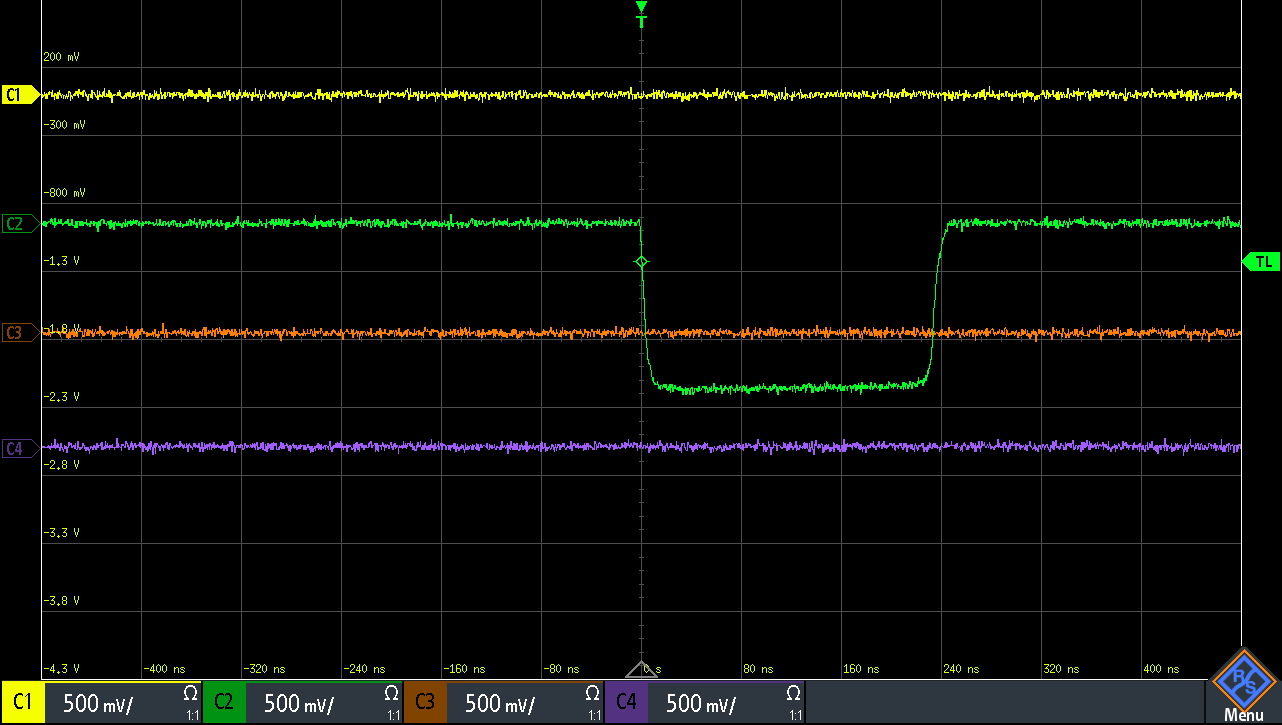
\includegraphics[width=\textwidth]{3DesignPrinciples/32Tritium_detector/1_coincidences.png}  
    \caption{\label{subfig:signalInOnePMT}}
    \end{subfigure}
    \hfill
    \begin{subfigure}[b]{0.45\textwidth}
    \centering
    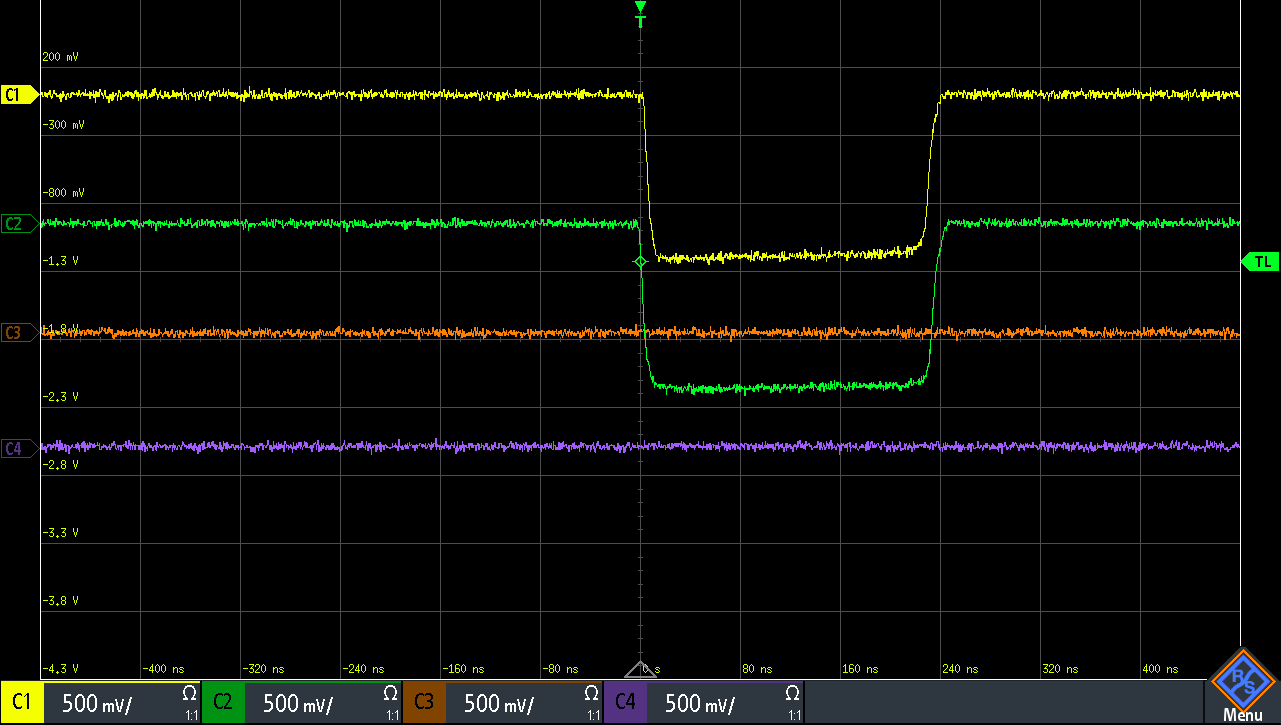
\includegraphics[width=\textwidth]{3DesignPrinciples/32Tritium_detector/2_coincidences_1.png}  
    \caption{\label{subfig:signalInTwoPMTOneDetector}}
    \end{subfigure}
    \hfill
    \begin{subfigure}[b]{0.45\textwidth}
    \centering
    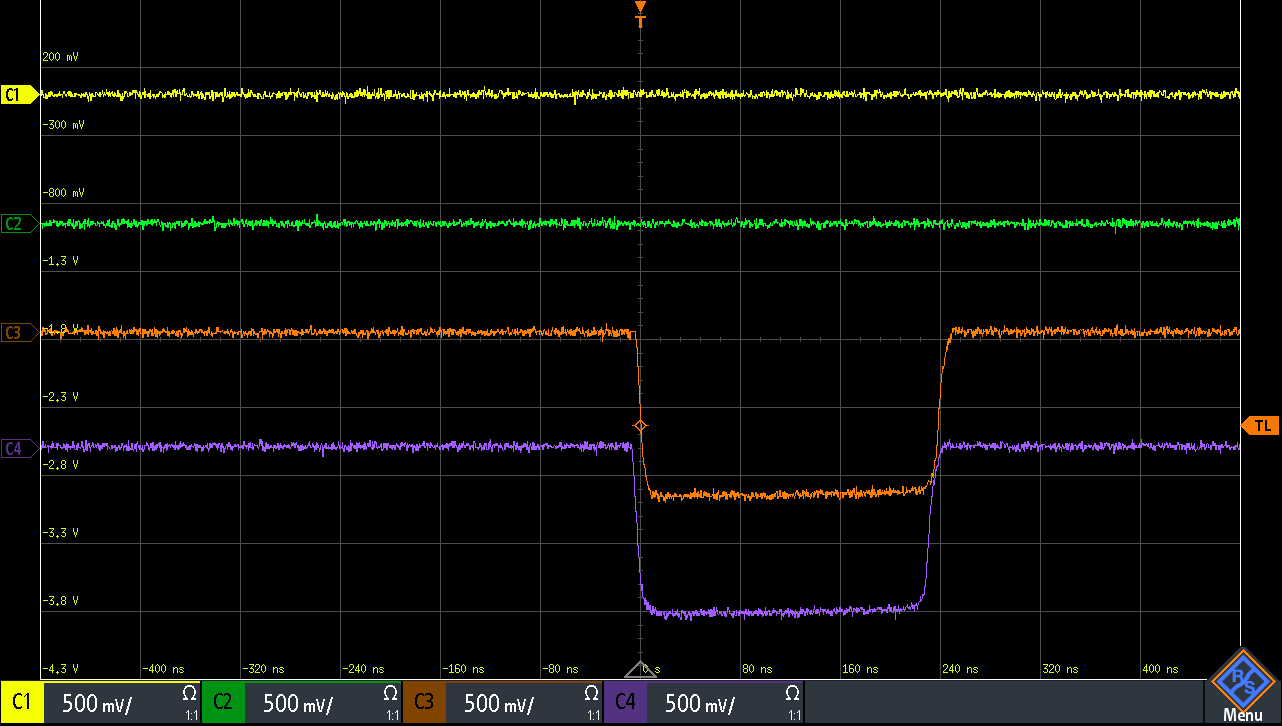
\includegraphics[width=\textwidth]{3DesignPrinciples/32Tritium_detector/2_coincidences_2.png}  
    \caption{\label{subfig:signalInTwoPMTOtherDetector}}
    \end{subfigure}
    \hfill
    \begin{subfigure}[b]{0.45\textwidth}
    \centering
    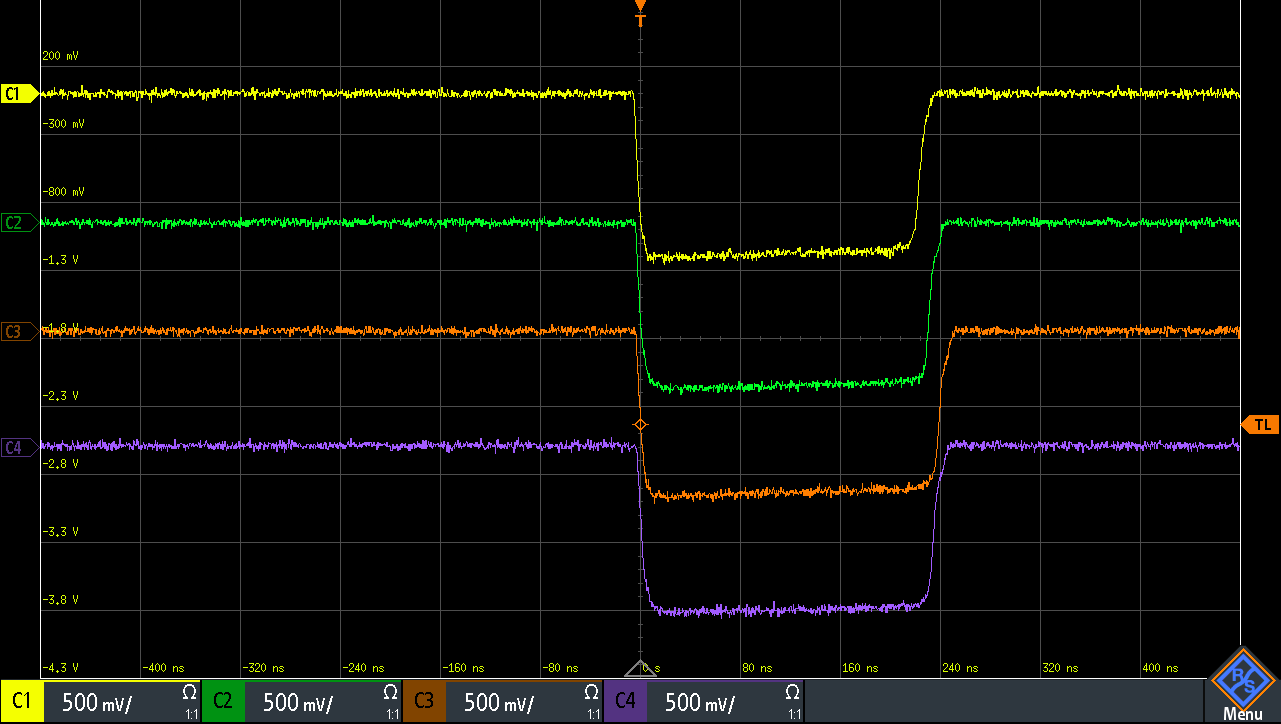
\includegraphics[width=\textwidth]{3DesignPrinciples/32Tritium_detector/4_coincidences.png}  
    \caption{\label{subfig:signalInAllPMTsBothDetector}}
    \end{subfigure}
 \caption{Different possibilities when time coincidences with PMTs are done. a) Event detected in only one PMT, one detector. b) Event detected in two PMTs, one detector. c) Event detected in two PMTs, other detector. d) Event detected in all PMTs, both detector.}
 \label{fig:DifferentCoincidences}
\end{figure}

\end{enumerate}

\item{} The logical output signal, is introduced in the Gate and Delay Generator, model 416A of the company ORTEC \cite{DataSheetGateAndDelay}, which gives a positive logical signal, called time windows, shown in Figure \ref{fig:InputSignalsMCA}, orange color, with a height of $8~\volt$ and width of $2~\mu\second$. This module is used to delay the time windows until it overlaps with the energy signal as it is shown in Figure \ref{fig:InputSignalsMCA}, orange signal.

\end{enumerate}

\end{enumerate}

As a final output of the electronics, a logical and analogical signals are obtained, shown in Figure \ref{fig:InputSignalsMCA}, which are recorded by the MCA 8000D, Pocket MCA from AMPTEK \cite{DataSheetMCA}. The analogical signal has information about the energy of the event and this is the signal which information is saved for later analysis. The logic signal (output from the Gate and Delay Generator module) indicates when the amplified signal must be saved.

\begin{figure}[htbp]
\centering
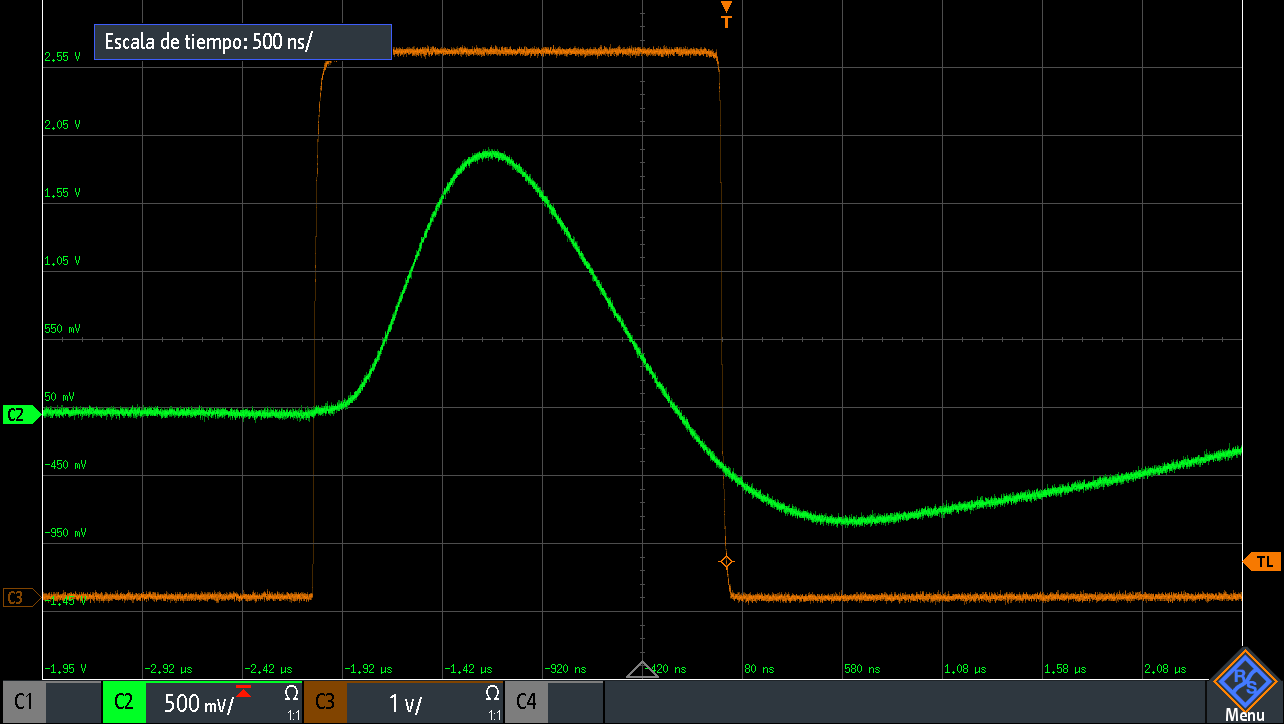
\includegraphics[scale=0.3]{3DesignPrinciples/32Tritium_detector/Input_MCA.png}
\caption{Signal amplified and logical gate (input signals of MCA).\label{fig:InputSignalsMCA}}
\end{figure}
			%\newpage
			
			\subsubsection[Electronics for SiPMs]{Electronics for SiPMs}\label{subsubsec:SiPMsElectronicalSystem}
			The SiPMs in the TRITIUM experiment are arranged in matrices of $4\times 4$. The electronic system chosen to process and analyze the output signals of the SiPM arrays is PETsys \cite{PETSYS}, displayed in Figure \ref{fig:PETSYS}, which is a commercial system prepared to work with SiPM matrices from Hamamatsu. PETsys provides time and energy digitalization, including the charge integrations QDCs\footnote{charge-to-digital converter} and TDCs\footnote{time-to-digital converter}, resulting in a complete acquisition and digitization system capable of working with up to 1024 SiPM. This system consists of a basic board to which 16 different SiPM matrices can be connected with up to 64 SiPM per matrix. This number of channels is needed in the TRITIUM project because, as shown in section \ref{sec:TritiumMonitor}, the TRITIUM monitor consists of a large number of SiPM matrices with 16 channels per matrix.

\begin{figure}[h]
\centering
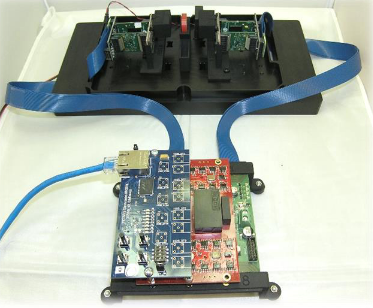
\includegraphics[scale=0.8]{3DesignPrinciples/32Tritium_detector/PETSYS_System.png}
\caption{Different parts of PETsys system\label{fig:PETSYS}~\cite{PETSYS}.}
\end{figure}
Although the capacity provided by PETsys should be enough for the requirements of the TRITIUM project, TRITIUM is a modular detector with scalable sensitivity. This means that, if an inprovement of TRITIUM limits is needed to improve its sensitivity or to further reduce the background, more photosensors would be needed. Therefore, the electronics should be able to increase its capacity in a scalable way. This requeriment is fulfilled by PETsys since it has an additional module, called Clock and Trigger, to which up to sixteen different PETsys basic boards can be connected. Theses sixteen PETsys basic boards are read in parallel, giving a total system capacity of reading 256 SiPM matrices (16384 SiPMs\footnote{$1024\cdot{}16 = 16384$}). 

PETsys software is based on C++ and Python scripts to drive the main tasks required, such as time coincidence options between SiPM (or even SiPM matrices) or energy discrimination. This software is open source, giving the possibility to modify the current scripts or to develop others with additional functions. PETsys has a time resolution better than $30~\pico\second$ which is one of the best time resolutions of commercial systems available and its price is around $10$\euro$/$ channel, which is cheaper than similar electronic systems.

As reported in section \ref{sec:CharacterizationSiPM}, the SiPM matrix temperature is an important parameter. The PETsys system has the ability to monitor the temperature of the SiPM matrices and ASICS employed to control them. Temperature monitoring is important to ensure the correct functioning of both photosensors and system. PETsys has the possibility of developing new scripts to implement the stabilization method of the SiPM gain reported in section \ref{sec:CharacterizationSiPM}.

Some characterization measurements were carried out using the PETsys system to ensure that the system works properly but the SiPM characterization was carried out at the level of a single channel (individual SiPM). The reason is that the output information of PETsys is already integrated and digitized, so it does not allow the SiPM to be calibrated. Therefore, to characterize a SiPM, a different electronic system was used to read up to eight different SiPMs. This system consists of a PCB that provides the SiPM bias voltage and reads the SiPM output signal. An example of the electronic scheme (provided by Hamamatsu) in which this PCB is based is shown in Figure \ref{fig:PCBSiPM}.

\begin{figure}
\centering
    \begin{subfigure}[b]{0.5\textwidth}
    \centering
    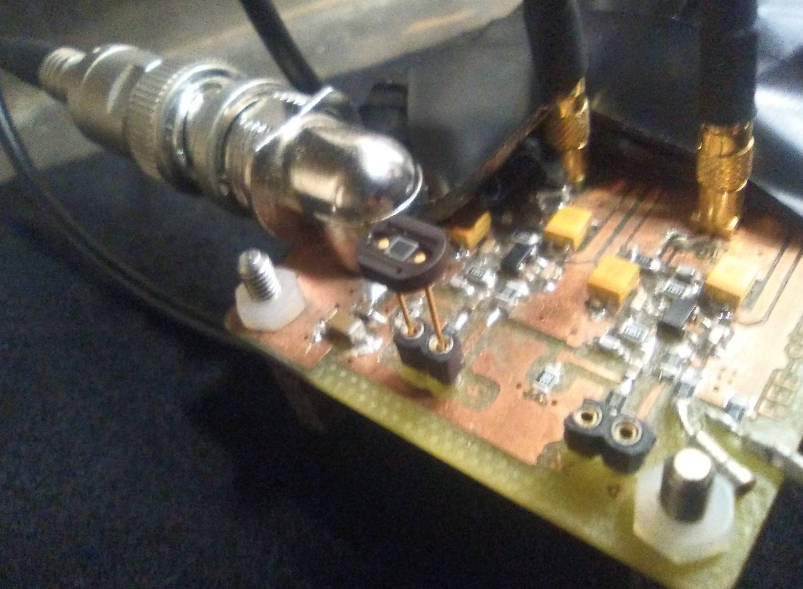
\includegraphics[width=\textwidth]{3DesignPrinciples/32Tritium_detector/SiPMPCB.png}  
    \caption{\label{subfig:ElectronicBoardSiPM}}
    \end{subfigure}
    \hfill
    \begin{subfigure}[b]{0.45\textwidth}
    \centering
    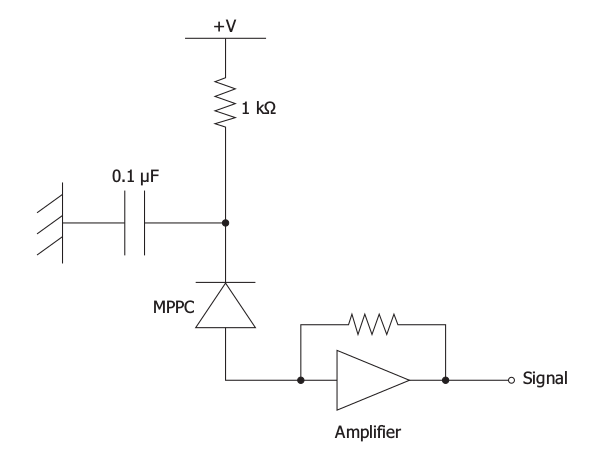
\includegraphics[width=\textwidth]{3DesignPrinciples/32Tritium_detector/ElectronicSchemePCBSiPM.png}  
    \caption{\label{subfig:ElectronicSchemePCBSiPM}}
    \end{subfigure}
    \hfill
 \caption{a) Electronic board used to provide the SiPM bias voltage and to read the SiPM output signal. b) Electronical scheme in which this PCB is based.}
 \label{fig:PCBSiPM}
\end{figure}
The PCB was feed at $\pm6~\volt$ using the voltage source ISOTECH, model IPS-4303 \cite{VoltageSourceISOTECH} and the SiPM was feed using the electrometer KETHLEY, model 6517B \cite{VoltageSourceKethley}, that achieves a resolution of $1~\milli\volt$, low enough to ensure that this voltage variations does not affect the SiPM gain. The output signal of this PCB is connected to an oscilloscope, model WwaveRunner 625Zi from TELEDYNE LECROY \cite{OscilloscopeIFIMED} that records the data which were subsequently analized by ROOT\footnote{ROOT is a framework for data processing, based on C ++ and object-oriented technology, developed at CERN and widely used in nuclear and particle physics.} scripts.
			%\newpage		
		
	\section{The Water Purification System}\label{sec:UltraPureWaterSystem}
	%\input{./Sections/3Design_Principles/33UltraPureWaterSystem} 
	%\newpage
		
		\subsection{Objectives}\label{subsec:IntroductionWaterSystem}
		The water samples, which will be introduced into the TRITIUM detector to be measured, are taken directly from the Tajus river, 4 km downstream from the place where the Almaraz Nuclear Power Plant releases the cooling water. This sample, as it was verified by a detailed analysis shown in section \ref{sec:CharacterizationUltraPureWaterSystem}, contains many dissolved elements such as minerals, organic deposits, and living matter dissolved in the water. These dissolved items need to be deleted for several reasons:

\begin{enumerate}

\item{} The mean free path of tritium electrons in water is around $5~\mu\meter$ and even less in solid materials like organic material. Tritium decay electrons have to reach the fiber to be detected and, consequently, the detector must be kept very clean. If the analyzed water sample contains particles that may be deposited on the fibers, a layer of matter could be formed, preventing tritium decay electrons from reaching the fibers and reducing drastically the tritium detection efficiency.

\item{} The tritium monitor does not have any spectrometric capabilities that could be used to distinguish tritium from other radioactive elements from minerals dissolved in the water.

\end{enumerate}

The water purification system was designed to remove organic matter and mineral particles with a size of up to $1~\mu\meter$. Hence, this filtering should keep unchanged the tritium level in the water. 

%Since tritium is the only radioactive element that can be practically equal to water (when it is in the $\ce{HTO}$ form, the majority form in wihch tritium are present in the water sample), with this process we remove all particles radioactive elements other than tritium and the amount of tritium present in the sample is not affected



%In summary, the ultrapure water system is used to keep our detector clean, ensuring the stability of its detection efficiency and to eliminate all radioactive particles other than tritium. %maintaining the activity of the tritium in the sample. Both reasons has been tested with experimental measurements, shown in secton \ref{sec:CharacterizationUltraPureWaterSystem}. 
		%\newpage
					
		\subsection{Design of the Water Purification System}\label{subsec:SetUpWaterSystem}
		The requeriments of this water treatment device are:

\begin{itemize}

\item{} to obtain a high degree of purification of the processed water sample, reducing its conductivity by approximately two orders of magnitude (from $1000~\mu$S$/\cm$ to $10~\mu$S$/\cm$)

\item{} to require of low maintenance (low cost  and low manpower)

\item{} to install a remote control device with probes and valves contolling by software.
\end{itemize}

The LARUEX laboratory in Extremadura, one of the six collaborators of the TRITIUM experiment, has designed, developed and built the ultrapure water system, a scheme of which is shown in Figure \ref{fig:WPSScheme}.

\begin{figure}[htbp]
\centering
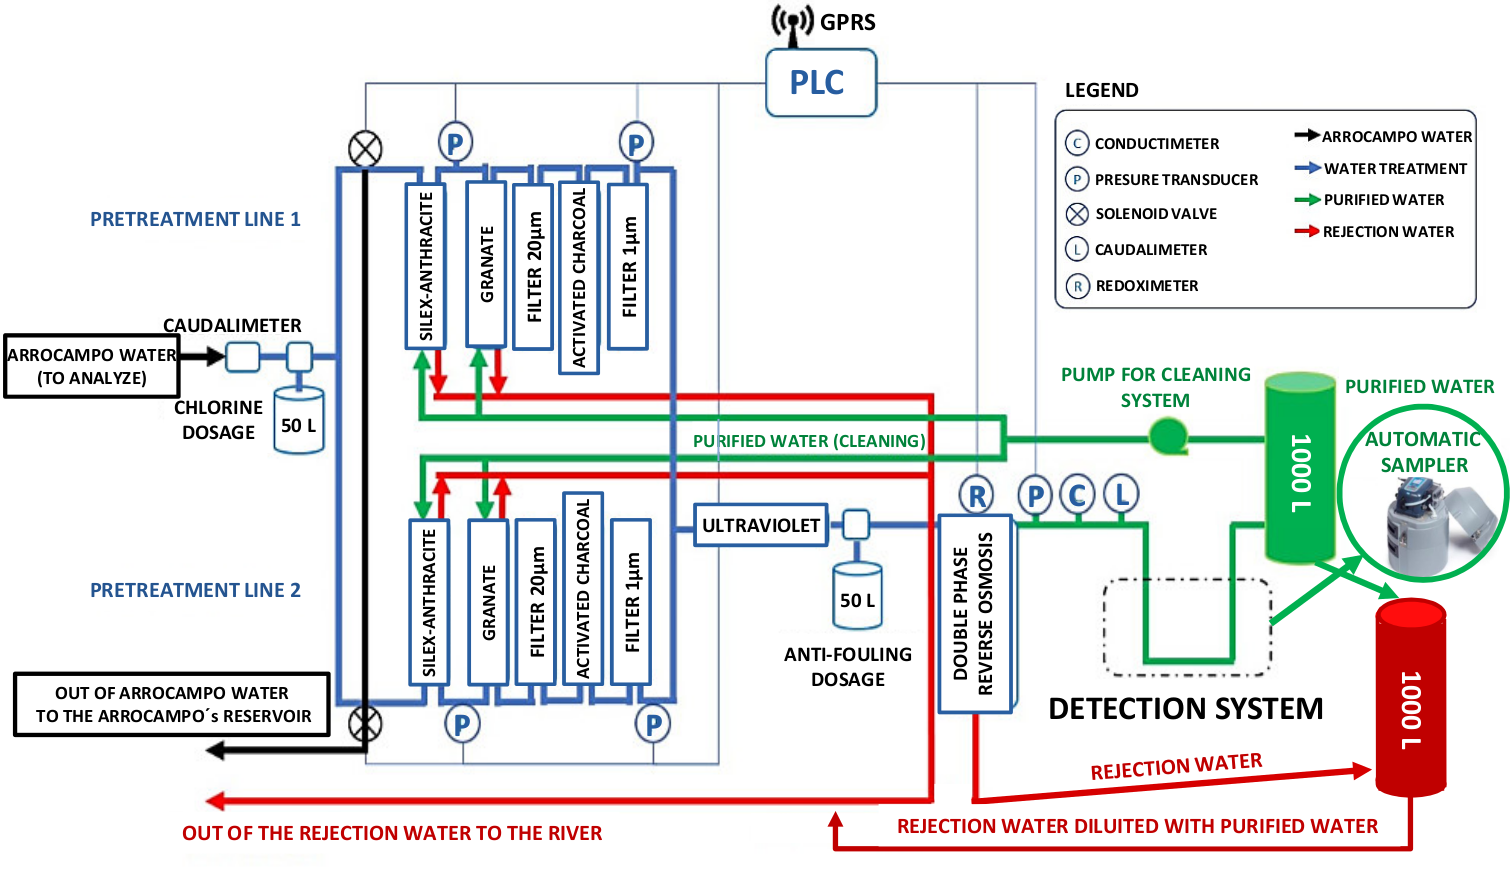
\includegraphics[scale=0.25]{3DesignPrinciples/33UltraPureWaterSystem/SchemeUltraPureWaterSystem.png}
\caption{Scheme of water purification system.\label{fig:WPSScheme}}
\end{figure}

This system is installed in the Arrocampo dam and consists of four different consecutive stages:

\begin{enumerate}
\item{} The raw water from the Tagus River passes through two different filters, the first made of silex-anthracite and the second of garnet, with which a rough filtering is made (the largest particles are eliminated). This system has two parallel lines and implements self-cleaning by injecting ultrapure water in the opposite direction.

\item{} The outlet water sample of the first stage, called fine filtration stage, passes through a $20~\mu\meter$ filter (formed by a synthetic mesh) and activated charcoal filters (one per line) that removes chlorine and iron particles.

\item{} The outlet water of the second stage passes through a super-fine filtering consisting of a $1~\mu\meter$ filter, formed of a dense polypropylene mesh and UV lamps. The first filter removes all the particles up to diameters of $1~\mu\meter$ and the UV lamps remove the organic matter present in the sample.

\item{} Finally, the water is introduced in the last stage, double-phase reverse osmosis, that reduces the conductivity of the water to about $5~\mu$S$/\cm$. It was verified that a conductivity of $10~\mu$S$/\cm$ is achieved with only one module of reverse osmosis, enough for the needed conditions of tritium detector. Therefore, only one module of reverse osmosis is used, reducing the power consumption of the system.

\end{enumerate}

As a result of the purification process, besides the ultrapure water that is introduced into TRITIUM detector, a rejection water, with conductivities greater than the original water containing the particles extracted from the ultrapure water is produced.

The ultrapure water system is able to process up to $0.850~\meter^3/\hour$ with a single line operating or $1.480~\meter^3/\hour$ with both, greatly overestimating the requirements of the tritium detector. 

The software used for remote controlling of the ultrapure water system is Siemens PLC, that gives the information such as the state of the valves, the pressure probes or water production in real time. 

The appendix \ref{App:UltraPureWaterSystem} contains several pictures of different parts of this system, installed in Arrocampo dam.
		%\newpage	
	
	\section{The Background Rejection System}\label{sec:IntroductionBackground}
	The aim of the background rejection system is to reduce the radioactive and cosmic background that affects to the TRITIUM monitor. The TRITIUM project follows the ALARA principle for the tritium activity measurement, that is, to measure tritium activity "as low as reasonably achievable". The detection limit of tritium activity is set by the uncertainty in the activity of the background of the natural radioactivity measured by the TRITIUM detector, since tritium activities below this uncertainty cannot be distinguished from the background. Therefore, the background uncertainty must be reduced as much as possible. The total uncertainty is the quadratic sum of all the different uncertainties related to the measurement, i.e., the statistical uncertainty\footnote{Uncertainty due to the statistical nature of the radioactivity process}, $\sigma_{st}$, the systematic uncertainty\footnote{uncertainty due to the manufacturing process of the detectors}, $\sigma_{si}$, etc. Because of the Poissonian nature of the process, the statistical uncertainty is given by the square root of the measured activity, $A_{m}$, which can be reduced by minimizing detected background events.

\begin{equation}
\sigma_{T}^2 = \sigma_{st}^2 +\sigma_{si}^2; \qquad \qquad \sigma_{st;bak} = \sqrt{A_{m;bak}}
\label{eq:SquareSumUncerainty}
\end{equation} 

The background rejection system of the TRITIUM monitor reduces the background activity measured by the TRITIUM detector, minimizing the statistical component of the background uncertainty.

The background of TRITIUM has two different sources. On the one hand, radioactive elements that are present in the crust of the Earth, mainly $\ce{^{40}K}$ and elements from the four different natural radioactive series, shown in Table \ref{tab:NaturalRadioactiveSeries}. On the other hand, the cosmic ray radiation. The primary cosmic radiation, of extra-terrestrial origin, is composed of high-energy particles, mainly protons and $\alpha$ particles, which interact with the Earth's atmosphere and generate a shower mainly composed by muons, electrons, photons and neutrons.

\begin{table}[htbp]
\centering{}%
\begin{tabular}{lcccc}
\toprule 
Mass Num. & Series & Primary & Half life (y) & Final \tabularnewline
\midrule
\midrule 
4n & Thorium & $\ce{^{232}Th}$ & $1.41 \cdot{} 10^{10}$ & $\ce{^{208}Pb}$ \tabularnewline
4n+1 & Neptunium & $\ce{^{237}Np}$ & $2.14 \cdot{} 10^{6}$ & $\ce{^{209}Pb}$ \tabularnewline
4n+2 & Uranium-Radium & $\ce{^{238}U}$ & $4.51 \cdot{} 10^{9}$ & $\ce{^{206}Pb}$ \tabularnewline
4n+3 & Uranium-Actinium & $\ce{^{235}U}$ & $7.18 \cdot{} 10^{8}$ & $\ce{^{204}Pb}$ \tabularnewline
\bottomrule
\end{tabular}
\caption{Classification of natural radioactive series \cite{NaturalRadioactiveSeries1, NaturalRadioactiveSeries2}. The information displayed for each radioactive series is the multiplicity of the mass number, the name of the series, the primary and final element, and the half-life of the primary element.}
\label{tab:NaturalRadioactiveSeries}
\end{table}
Cosmic radiation depends on several parameters like the longitude, latitude, and the solar activity cycle. The spatial distribution of cosmic rays, mainly muons, follows a $cos^2(\theta)$ distribution with the zenith angle. 

Two different techniques are employed for background suppression:

\begin{enumerate}

\item{}  The soft background component, with energy below $200~\MeV/$nucleon, is stopped by a lead castle, described in section \ref{subsec:SetUpPassiveShield},

\item{} The hard background component, with energy greater than $200~\MeV/$nucleon, is much more difficult to stop and the technique employed is the use of a cosmic veto in anti-coincidence with the TRITIUM detector, reported in section \ref{subsec:SetUpActiveShield}. %that is, we will save the measured tritium event just when we don't measure any hard cosmic event in time coincidence.

\end{enumerate} 
	%\newpage
	
		\subsection{Passive Shield}\label{subsec:SetUpPassiveShield}
		The soft background component is suppressed by a lead shield inside which the TRITIUM detector is placed. This lead shield is efficient for suppressing radiation that originates from the Earth's natural radioactivity and the soft component of cosmic radiation with energies below $200~\MeV$. This lead shield consists of $158$ low intrinsic radioactivity lead bricks of $25~\mm$ thickness. The bricks are chevron shaped, as shown in Figure \ref{fig:LeadBrick}, specially designed for a perfect fit and easy assembly. As can be seen in Figures \ref{subfig:TwoLayers} and \ref{fig:LeadBricksAndArrangement}, these lead bricks are arranged in two layers with a total thickness of $50~\mm$. 
\begin{figure}[h]
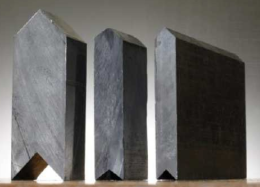
\includegraphics[scale=0.6]{3DesignPrinciples/34BackgroundRejectionSystem/LeadBricks.png}
\centering
\caption{Lead bricks.\label{fig:LeadBrick}}
\end{figure}
\begin{figure}[h]
\centering
    \begin{subfigure}[b]{0.5\textwidth}
    \centering
    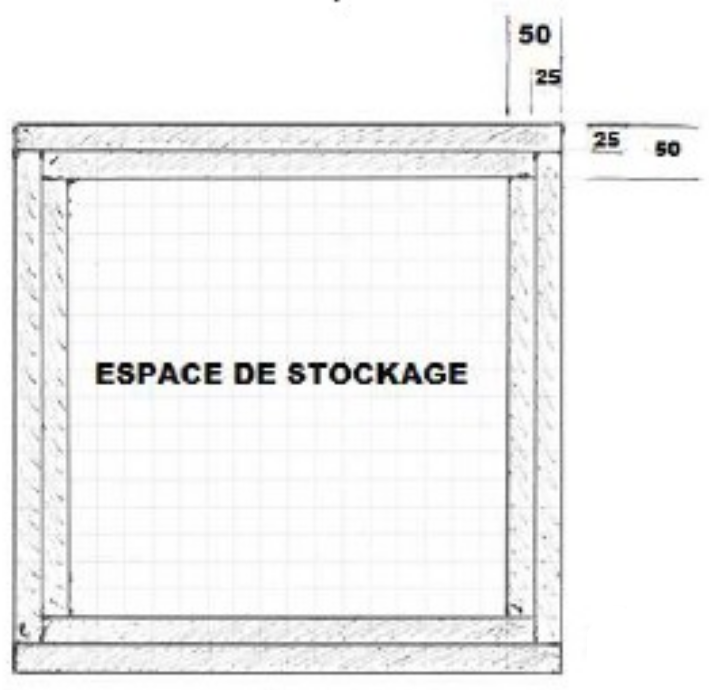
\includegraphics[width=\textwidth]{3DesignPrinciples/34BackgroundRejectionSystem/TwoLayers.png}  
    \caption{\label{subfig:TwoLayers}}
    \end{subfigure}
    \hfill
    \begin{subfigure}[b]{0.4\textwidth}
    \centering
    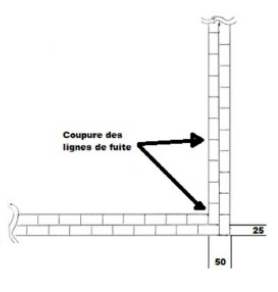
\includegraphics[width=\textwidth]{3DesignPrinciples/34BackgroundRejectionSystem/TwoLayers2.png}  
    \caption{\label{subfig:TwoLayers2}}
    \end{subfigure}
 \caption{Two layers for the lead bricks of the shield. a) General view of the lead castle. b) Detail of the lead brick arrangement.}
 \label{fig:LeadBricksAndArrangement}
\end{figure}
An aluminium structure capable of supporting the total weight of $2.4$ tons of lead bricks, shown in Figure \ref{fig:AluminiumStructure}, was designed by the Mechanical Engineering Department of the CENBG.
\begin{figure}
\centering
    \begin{subfigure}[b]{0.5\textwidth}
    \centering
    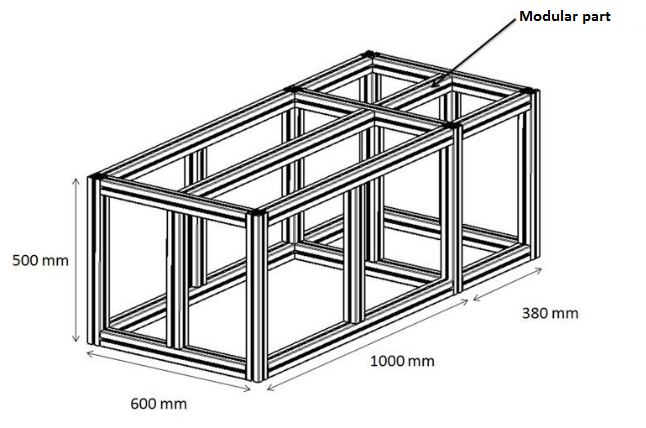
\includegraphics[width=\textwidth]{3DesignPrinciples/34BackgroundRejectionSystem/AluminiumStructureScheme.png}  
    \caption{\label{subfig:AluminiumStructureScheme}}
    \end{subfigure}
    \hfill
    \begin{subfigure}[b]{0.45\textwidth}
    \centering
    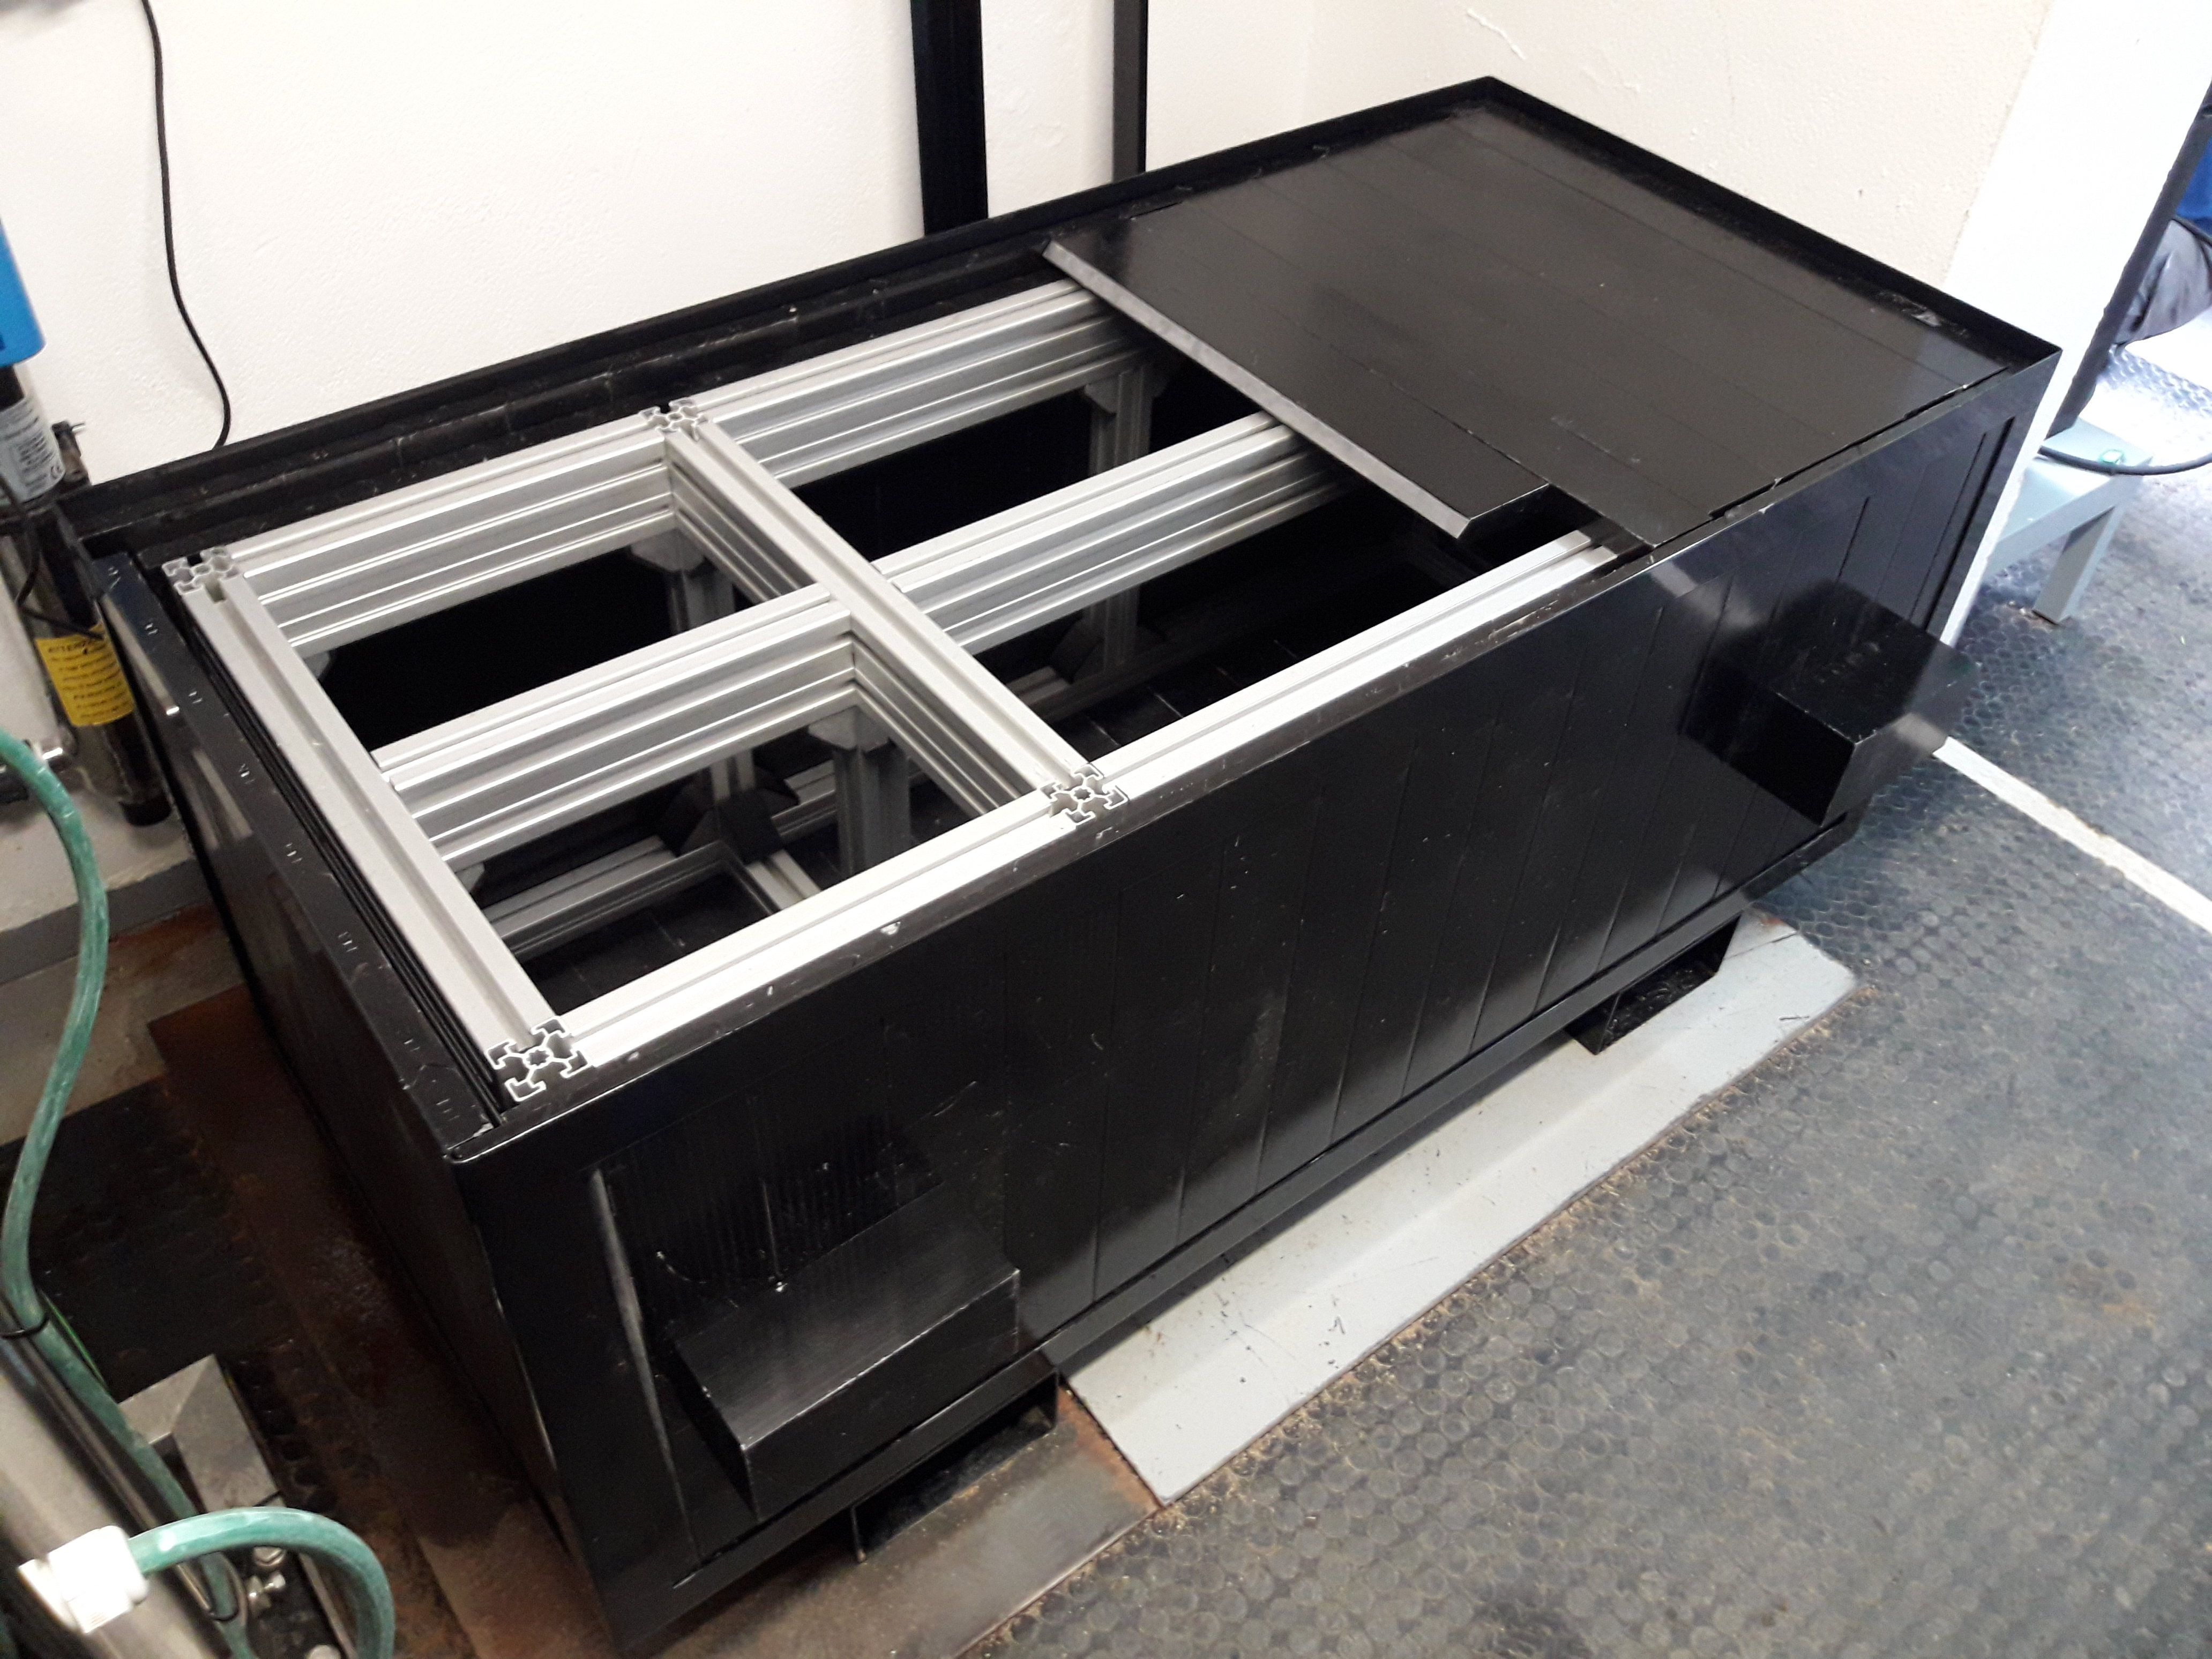
\includegraphics[width=\textwidth]{3DesignPrinciples/34BackgroundRejectionSystem/AluminiumStructure.jpg}  
    \caption{\label{subfig:AluminiumStructure}}
    \end{subfigure}
    \caption{a) Scheme of the aluminium structure of the shield. b) The lead shield partially mounted.}
 \label{fig:AluminiumStructure}
\end{figure}
The internal room of the lead shield is divided into two parts, as indicated in Figure \ref{fig:AluminiumStructure}. The larger one has internal dimensions of $90.5 \times 41 \times 51~\cm^3$ and is used to place the TRITIUM detector. The smaller one, with dimensions of $33 \times 41 \times 51~\cm^3$, contains the DAQ system of the detector. The external dimensions of the lead shield are $148 \times 60 \times 70~\cm^3$ and its total weight is $2.5$ tons.
		%\newpage
		
		\subsection{Active Shield}\label{subsec:SetUpActiveShield}
		As hard radiation cannot be stopped by a moderate lead thickness so cosmic vetos are employed, which consists of at least two complementary detectors in coincidence that reject events simoultaneously detected in both. 

As shown in Figure \ref{fig:VetoAndPrototype}, the two complementary detectors are placed one above and the other below the TIRTIUM detector. The distance between both detectors, $34.2~\cm$ for our latest prototype developed, is set by the TRITIUM prototype to be placed between both.

\begin{figure}[h]
\centering
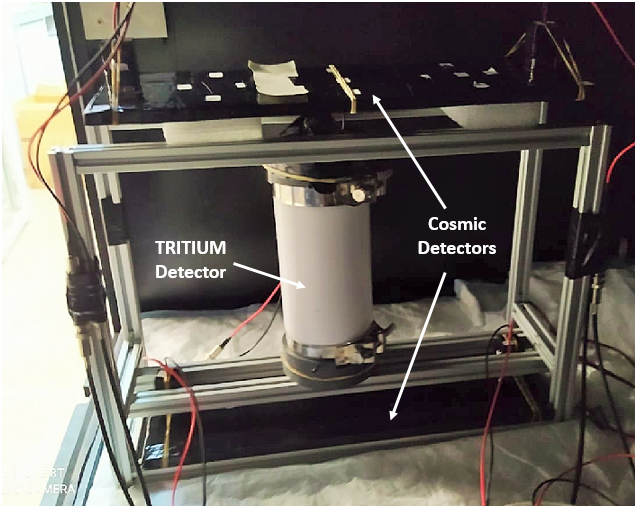
\includegraphics[scale=0.45]{3DesignPrinciples/34BackgroundRejectionSystem/Vetos_y_prototipo.png}
\caption{Cosmic veto and Tritium-IFIC 2 prototype in an aluminum mechanical structure developed by IFIC's mechanical engineering department.\label{fig:VetoAndPrototype}}
\end{figure}

A hard cosmic event simultaneous through both cosmic detectors is schematically shown in figure \ref{subfig:RealHardCosmicEvent}. Each cosmic detector has two photosensors so the electronic configuration given in Figure \ref{subfig:ElectronicConfiguraiton4PMT} is used in each active veto to make time coincidences. The TRITIUM detector is read out in anti-coincidence with the cosmic veto to rejected the hard cosmic events from the tritium measurement. Random coincidence from two different hard cosmic events, one in each detector, shown in Figure \ref{subfig:FakeHardCosmicEvent} are negligible. The expected hard cosmic rate at sea level for muons, main contributor, is $70~\meter^{-2}\second^{-1}\steradian^{-1}$ \cite{PDG, HardCosmicMuonRate}, that is $7\times 10^{-3}~\cm^{-2}\second^{-1}\steradian^{-1}$, shown in the cosmic rate plot of Figure \ref{fig:HardCoscmicRate}. As time coincidences are triggered by logical gates of about $10~\nano\second$, the probability of recording two different hard cosmic events in temporal coincidence is less than $10^{-9}$ which is not worth considering.

\begin{figure}
\centering
    \begin{subfigure}[b]{0.45\textwidth}
    \centering
    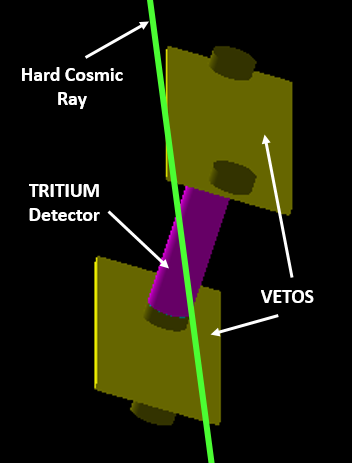
\includegraphics[width=\textwidth]{3DesignPrinciples/34BackgroundRejectionSystem/Real_Event.png}  
    \caption{Real hard cosmic event.\label{subfig:RealHardCosmicEvent}}
    \end{subfigure}
    \hfill
    \begin{subfigure}[b]{0.45\textwidth}
    \centering
    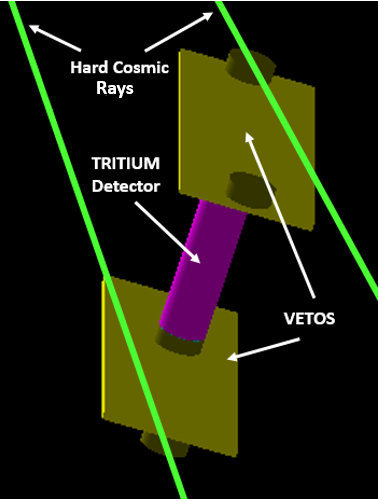
\includegraphics[width=\textwidth]{3DesignPrinciples/34BackgroundRejectionSystem/Fake_Event.png}  
    \caption{Fake hard cosmic event.\label{subfig:FakeHardCosmicEvent}}
    \end{subfigure}
   \caption{Hard cosmic events detected with the cosmic veto of TRITIUM: a) Affecting to the tritium measurement, b) Does not affecting to the tritium measurement.}
 \label{fig:HardCosmicEventsSimulation}
\end{figure}

\begin{figure}[h]
\centering
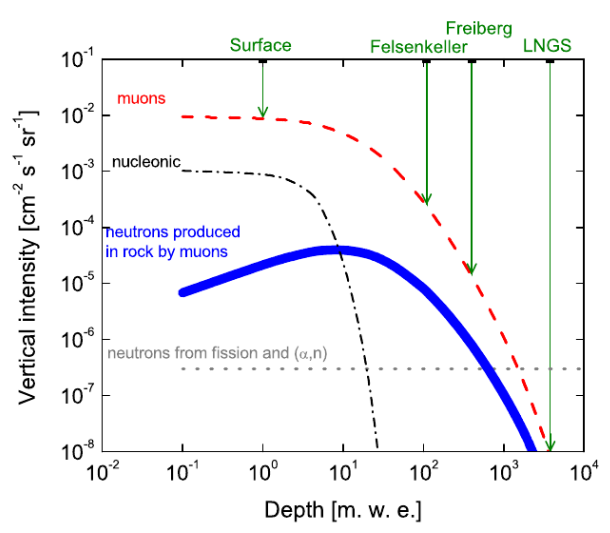
\includegraphics[scale=0.6]{3DesignPrinciples/34BackgroundRejectionSystem/HardCosmicRate.png}
\caption{Hard cosmic muon rate \cite{HardCosmicMuonRatePlot}.\label{fig:HardCoscmicRate}}
\end{figure}

The vetos are made of a plastic scintillator block from Epic-Crystal \cite{ScintillatorVeto}. Its properties are given in Table \ref{tab:ParametersScintillatorVeto} and its energy emission spectrum is displayed in Figure \ref{fig:EmissionEnergySpectrumVeto}.

\begin{table}[]
%%\centering
\begin{center}
\begin{tabular}{|c|c|c|}
%\hline
%Material & Refractive index \\
\hline \hline 
Base material & Polystyrene \\ \hline
Growth method & Polymeric \\ \hline
Density ($\gram/\cm^3$)& 1.05 \\ \hline
Refractive index & 1.58 \\ \hline
Soften temperature ($\degree$) & 75-80 \\ \hline
Light output (Anthracene) & 50-60\% \\ \hline
H/C raito & 1.1 \\ \hline
Emission peak (nm) & 415 (Blue) \\ \hline
Decay Time, (ns) & 2.4 \\ \hline
Hygroscopic & No \\ \hline
\end{tabular}
\caption{Properties of plastic scintillators from Epic-Crystals. \cite{ScintillatorVeto}}
\label{tab:ParametersScintillatorVeto}
\end{center}
\end{table}

\begin{figure}[]
\centering
\includegraphics[scale=0.35]{3DesignPrinciples/34BackgroundRejectionSystem/EmissionEnergySpectrumVetos.png}
\caption{Emission energy spectrum of the plastic scintillation used for the cosmic vetos.\label{fig:EmissionEnergySpectrumVeto}~\cite{ScintillatorVeto}}
\end{figure}

The energy spectrum has a peak very close to that of the scintillating fibers used, so the same photosensors are used to read out them. The dimensions of the scintillator block are $45 \cdot{} 17 \dot{} 1~\cm^3$ and they are wrapped by three different layers, teflon, aluminum and black tape, exhibited in Figure \ref{fig:LayersVeto}. These layers prevent external photons from reaching the scintillator plastic and avoid photons generated by the scintillator plastic from escaping before reaching the photosensor. Two $2.5\times 2.5 ~\cm^2$ windows are made on the wrapping to allow reading by the photosensors.


\begin{figure}
\centering
    \begin{subfigure}[b]{0.23\textwidth}
    \centering
    \includegraphics[width=\textwidth]{3DesignPrinciples/34BackgroundRejectionSystem/NoCoating.jpeg}  
    \caption{Scintillator without coating.\label{subfig:PlasticScintillatorNoCoating}}
    \end{subfigure}
    \hfill
    \begin{subfigure}[b]{0.23\textwidth}
    \centering
    \includegraphics[width=\textwidth]{3DesignPrinciples/34BackgroundRejectionSystem/TeflonCoating.jpeg}  
    \caption{Teflon coating.\label{subfig:PlasticScintillatorTeflon}}
    \end{subfigure}
    \hfill
    \begin{subfigure}[b]{0.23\textwidth}
    \centering
    \includegraphics[width=\textwidth]{3DesignPrinciples/34BackgroundRejectionSystem/AluminiumCoating.jpeg}  
    \caption{Aluminium coating.\label{subfig:PlasticScintillatorAluminium}}
    \end{subfigure}
    \hfill
    \begin{subfigure}[b]{0.23\textwidth}
    \centering
    \includegraphics[width=\textwidth]{3DesignPrinciples/34BackgroundRejectionSystem/BlackTapeCoating.jpeg}  
    \caption{Black tape coating.\label{subfig:PlasticScintillatorBlackTape}}
    \end{subfigure}
 \caption{Different layers used to cover of the cosmic veto.}
 \label{fig:LayersVeto}
\end{figure}

As previously mentioned, the expected hard cosmic rate at sea level is $7 \times 10^{-3}~\cm^{-2}\second^{-1}\steradian^{-1}$. Taking into account that the solid angle of our detectors is $\omega=0.5434$, calculated by integrating the solid angle of one scintillator on the other, and the area of the veto is $765~\cm^2$, the expected hard cosmic rate on our cosmic vetos should be $2,909~$event$/\second$. This is an important result which is used in section \ref{sec:TritiumActiveVeto} to determine the efficiency of the cosmic veto.
		\newpage
					
\chapter{TRITIUM Monitor R\&D}\label{chap:ResearchandDevelopment}
	%\section{Introduction}\label{sec:IntroCharacterisation}
	This chapter describes the characterization of the different parts of the TRITIUM monitor, including scintillating fibers, SiPMs, the water purification system and the background rejection system. This characterization is crucial to understand the behaviour of the different parts and the results of the monitor. Furthermore, several developments were made  to improve fundamental parameters of the TRITIUM monitor components to enhance their tritium sensitivity. All these studies were carried out inside a special light-tight box, called black box, to ensure that the detected photons come from the sources used, either LEDs or scintillators. In addition, as the energy response of plastic scintillators has a rather large uncertainty, most of the energy spectra are shown in ADC\footnote{ADC units are the internal units, called channels, in which an analog signal is digitized after an Analog-to-Digital Converter. The ADC units are proportional to the energy and the number of available channels depends on the bits used in its digitization.} channels, which are linearly proportional to energy.
	%\newpage
	
	\section{R\&D for the Scintillating Fibres}\label{sec:CharacterizationScintillatingFibers}
	This section reports experimental measurements of the scintillating fiber parameters that most affect the tritium detection, such as collection effficiency and conditioning uncertainty. Errors are included in all graphs displayed in this section but they are to small to be visible. Thousands of scintillating fibers are used in TRITIUM detector which were prepared and conditioned prior to characterization studies or tritium detection. Therefore, various mechanical and electronical devices were developed to automatically prepare many fibers at the same time.
		%\newpageand
		
		\subsection{Preparation of Scintillating Fibres}\label{subsec:SurfaceConditioningProcess}
		A surface-conditioning of the scintillating fibres, which consists in cleaving, polishing and cleaning, was implemented to improve their photon collection efficiency. These methods are described in the following subsections.


				
			\subsubsection{Cleaving of Scintillating Fibres}\label{subsubsec:CleavingProcess}
			The first step in the TRITIUM design was to choose the fibre length and the fibre diameter ($1$ or $2~\mm$) for which the signal of tritium events is optimized. For a given active area, the longer the fibres, the smaller the number of photosensors needed. However, in long fibres photons are reflected on their boundaries many times before reaching the photosensors, which may produce a deterioration in the tritium signal. To determine the optimal fibre length, several simulations, described in section \ref{subsec:FiberLengthSimulation}, were carried out using Geant4 \cite{Geant4WebPage}. It was concluded that the optimal fibre length for measuring tritium in water is around $20~\cm$, which is the fibre length used in the TRITIUM prototypes developed at IFIC and for most of the characterization studies carried out in this thesis. As the manufacturer \cite{SaintGobain} delivers $1~\meter$ long fibres, an effective cleaving technique had to be developed with stringent requirements on the cleaving quality, since this greatly affects the transmission of photons and, consequently, the detection efficiency of the TRITIUM detector. The cleaving must be done perpendicular to the fibre axis and with small uncertainty in the cleaving position to enable optimal coupling of the fibre to the photosensor. It is also important that the fibre integrity be preserved, without cracks or deformations that may contribute to photon loss. 

Cleaving plastic fibres is a current challenge. There are many different techniques such as milling, laser cleaving, focused-ion-beam, blade cleaving, etc. The blade cleaving technique was chosen because of its mechanical simplicity and because, unlike other techniques, it preserves the integrity of plastic fibres. Many commercial devices based on blade cleaving, such as the one provided by Thorlabs with a diamond tipped blade \cite{DiamondThorlabs}, or guillotines designed for industrial fibre optics \cite{GuillotineIFO}, were tested in an comprehensive study with unsuccessful results \cite{TFGAlberto}. As it can be seen in Figure \ref{fig:BadCleavesOfFibers}, commercial techniques produce deformations, cracks and imperfections so they do not yield results with the quality standard required for the detector.
\begin{figure}
\centering
    \begin{subfigure}[b]{0.5\textwidth}
    \centering
    \includegraphics[width=\textwidth]{4ResearchAndDevelopments/41Fibers/DeformationFiberEnds.png}  
    \caption{\label{subfig:FiberEndDeformation}}
    \end{subfigure}
    \hfill
    \begin{subfigure}[b]{0.45\textwidth}
    \centering
    \includegraphics[width=\textwidth]{4ResearchAndDevelopments/41Fibers/CracksEndFibers.png}  
    \caption{\label{subfig:FiberEndCracks}}
    \end{subfigure}
 \caption{Results of using commercial techniques for cleaving the scintillating fibres a) Fibre end deformation b) Fibre end cracks. Pictures taken with a microscope PB 4161 from EUROMEX.}
 \label{fig:BadCleavesOfFibers}
\end{figure}
Because commercial devices are not suitable for polymer fibres, a cleaving device, shown in Figure \ref{fig:CleaveTRITIUMDevice}, was designed and built at IFIC laboratory.
\begin{figure}
\centering
    \begin{subfigure}[b]{0.5\textwidth}
    \centering
    \includegraphics[width=\textwidth]{4ResearchAndDevelopments/41Fibers/CuttingDevice.png}  
    \caption{\label{subfig:CleaveTRITIUMDevice1}}
    \end{subfigure}
    \hfill
    \begin{subfigure}[b]{0.45\textwidth}
    \centering
    \includegraphics[width=\textwidth]{4ResearchAndDevelopments/41Fibers/Cleaving_machine_ZOOM.png}  
    \caption{\label{subfig:CleaveTRITIUMDeviceZOOM}}
    \end{subfigure}
 \caption{Plastic fibre cleaver developed in TRITIUM project. \label{fig:CleaveTRITIUMDevice}}
\end{figure}
This device consists of an aluminium plate endowed with fourteen grooves to accommodate the fibres. A thin razor blade attached to a mobile piece is used to cleave the fibres. The perpendicular cleave, which is one of the requirements, can be ensured since the moving piece to which the blade is attached is placed perpendicular to the fibre axis. The blade used is a typical commercial razor blade, of $0.1~\mm$ thickness, which is the thickness that gave the best results. The blade was positioned with a $5\degree$ inclination with respect to the horizontal axis since it was found in several studies that this helps to obtain a less aggressive and cleaner cleave \cite{AngleBlade, TemperatureBlade}. As it can be seen in Figure \ref{fig:CleavingFiberEnd}, the integrity of the fibre is preserved and no deformation is observed. However, it can be noticed some tears on the clad, but it is reported in section \ref{subsubsec:CharacterizationFibers} that these tears affect negligibly the photon collection. 

An additional parameter that could affect the cleaving quality of the fibre ends is the temperature of both fibre and blade. A study was carried out in which both were subject to different temperatures, from room temperature to $110\celsius$. No significant conclusions were obtained \cite{TFGAlberto}. Thus, the cleaving process was carried out at room temperature to make the cleaving process easier.

\begin{figure}[h]
\centering
\includegraphics[scale=0.75]{4ResearchAndDevelopments/41Fibers/CutEndFiberGood.png}
\caption{Fibre end after cleaving process using the home-made cleaver. Pictures taken with the microscope PB 4161 from EUROMEX.\label{fig:CleavingFiberEnd}}
\end{figure}

A second L-shaped aluminium plate with grooves was attached to the first one (see Figure \ref{fig:CleaveTRITIUMDevice}) to set accurately the length of the fibres to $200~\mm$, with an uncertainty of $\pm 1~\mm$.
			%\newpage
			
			\subsubsection{Polishing Scintillating Fibres}\label{subsubsec:PolishingProcess}
			As can be seen in Figure \ref{fig:CleavingFiberEnd}, a slightly darkened zone at the bottom of the fiber is observed in most of the cases. This is an unavoidable effect of the cleaving process on plastic fibers, which generates non polished end-surfaces. To restore, the polishing process implemented by Thorlabs was applied \cite{DiamondThorlabs}. 

\textbf{Manual Polishing Method.}

The Thorlabs polishing method, illustrated in Figure \ref{fig:HandPolishingMethod}, consists in a kit based on a special fiber connector which is used for rubbing the fibers with five different polishing papers made of aluminium  oxyde grains, with a decreasing grain size, $30~\mu\meter$, $20~\mu\meter$, $12~\mu\meter$, $5~\mu\meter$ and $0.3~\mu\meter$. To polish the fiber, a shape of an 8 must be outlined during 2 minuts (approximately 120 movements). 

\begin{figure}[h]
\centering
\includegraphics[scale=0.75]{4ResearchAndDevelopments/41Fibers/Hand_Polishing_Kit.png}
\caption{Manual polishing method implemented by Thorlabs.\label{fig:HandPolishingMethod}}
\end{figure}
The result obtained after polishing is shown in Figure \ref{subfig:PolishFiberEnd}, where it can be noticed that the darkened zone has completely disappeared and the fiber end is uniform, which favors optimal coupling and transmision of photons of the scintillating fibers to the photodetectors.

\begin{figure}
\centering
    \begin{subfigure}[b]{0.5\textwidth}
    \centering
    \includegraphics[width=\textwidth]{4ResearchAndDevelopments/41Fibers/CutEndFiberGood.png}  
    \caption{\label{subfig:CleaveFiberEnd}}
    \end{subfigure}
    \hfill
    \begin{subfigure}[b]{0.45\textwidth}
    \centering
    \includegraphics[width=\textwidth]{4ResearchAndDevelopments/41Fibers/CutAndPolishedFiberEnd.png}  
    \caption{\label{subfig:PolishFiberEnd}}
    \end{subfigure}
 \caption{Result of the polishing process. a) Fiber end after cleaving b) Fiber end after cleaving and manual polishing with Thorlabs technique. Pictures taken with the microscope PB 4161 from EUROMEX.}
 \label{fig:ResultofPolishingProcess}
\end{figure}

\textbf{Automatic Polishing Machine.}

The main drawback of the manual polishing method is that it takes more than 10 minutes to polish a fiber, an unaffordable time to polish the thousands of fibers needed for the TRITIUM detector (see section \ref{sec:TritiumMonitor}). This is why an automated polishing process was developed within this thesis work. The goal of this effort was to ensure a better light coupling and transmission of light of the scintillating fibers to the photosensors. 


%As mentioned above, tens of thousands of fibers had to be prepared and conditioned for the TRITIUM monitor\footnote{Tritium monitor is composed of several modules based on hundred of scintillating fibers.} (see section \ref{sec:TritiumMonitor}). Cleaving this large number of fibers with out home-made cleaving device was a relatively fast process. Polishing them however is quite time consuming, as it takes ten minutes to hand polish one fiber. Hand polishing thoudands of fibers,  would result in an unaffordable amount of time. This is why an automated polishing process has been developed within this thesis work. The goal of this effort was to ensure a better light coupling and transmission of light of the scintillating fibers to the photosensors. 

A machine was designed, built and tested in the laboratory for automatically polishing of up to one hundred plastic scintillating fibers at the same time and it is easily scalable to larger number of fibers.

\begin{figure}[h]
\centering
\includegraphics[scale=0.75]{4ResearchAndDevelopments/41Fibers/GeneralViewPolishingMchine.png}
\caption{Polishing machine developed for TRITIUM.\label{fig:GeneralViewPolishingMachine}}
\end{figure}
This automatic polishing machine, displayed in Figure \ref{fig:GeneralViewPolishingMachine}, consists of two main parts: 1) A polishing table, where the fibers are polished 2) The electronics, based on Arduino technology, that operates the movement of the polishing paper:

\begin{enumerate}
\item{} The polishing table, shown in Figure \ref{subfig:PolishingTable}, is composed of two parts, a static part, where the fibers are fixed, and a movable part on bottom of the previous one, where the polishing papers are fixed. It was decided to establish the polishing movement on the plate with the polishing sheets, because of its lighter weight and in order to avoid possible damaging movements to the fibers.

The static part (the fiber holder plate), shown in Figure \ref{subfig:PolishingTable}, consists of a plastic piece built with a 3D printer and locked to the system by four vertical screws. There are two nuts on each screw used to set the relative height and the inclination of fibers relative to the polishing papers. This piece contains one hundred holes in which a hundred fibers are lodged. 

As the fibers are too light ($0.16~\gram$) to make by gravity the necessary pressure on the polishing paper, a plastic belt and a piece of metal with a weight of about $1.5~\gram$ were attached to the individual fibers, as shown in Figure \ref{subfig:FiberMetailcPiece}, to increase their contact pressure, in a similar way as with the manual polishing connectors. 

The movable part of the polishing table consists of a flat PMMA plate of $18 \times 18~\cm^2$ to which the polishing paper is attached. This part is locked to structure \cite{StructureAxis} that contains two horizontal screws, perpendicular to each other, which allow its movement in the XY plane (horizontal plane), as shown in Figure \ref{subfig:HorizontalAxis}.

The polishing system contains several subminiature switches with high repeat accuracy, model DB1 6A250, mounted on a piece made with a 3D printer, shown in Figures \ref{subfig:PolishingTable}, \ref{subfig:HorizontalAxis} and \ref{subfig:3DSwitchPiece}, which are used to find the origin of coordinates when the system is reinitiated and to stop the movable part when the end of the path is reached. 

\begin{figure}
\centering
    \begin{subfigure}[b]{0.55\textwidth}
    \centering
    \includegraphics[width=\textwidth]{4ResearchAndDevelopments/41Fibers/PolishingTable.png}  
    \caption{\label{subfig:PolishingTable}}
    \end{subfigure}
    \hfill
    \begin{subfigure}[b]{0.3\textwidth}
    \centering
    \includegraphics[width=\textwidth]{4ResearchAndDevelopments/41Fibers/PieceOfFiber.png}  
    \caption{\label{subfig:FiberMetailcPiece}}
    \end{subfigure}
    \hfill
    \begin{subfigure}[b]{0.55\textwidth}
    \centering
    \includegraphics[width=\textwidth]{4ResearchAndDevelopments/41Fibers/HorizontalAxis2.png}  
    \caption{\label{subfig:HorizontalAxis}}
    \end{subfigure}
    \hfill
    \begin{subfigure}[b]{0.4\textwidth}
    \centering
    \includegraphics[width=\textwidth]{4ResearchAndDevelopments/41Fibers/Switch.png}  
    \caption{\label{subfig:3DSwitchPiece}}
    \end{subfigure}
 \caption{Components of the fiber polishing machine. a) Polishing table. b) Fiber with ballast metal piece. c) Horizontal screws and PMMA plate. d) A movement switch with its cables inserted inside its holding piece.}
 \label{fig:PolishingTable}
\end{figure}

\item{} The electronics, shown in Figure \ref{fig:ElectronicSystemPolishingMachine}, which controls the automatic movement of the polishing paper, is based on Arduino technology. It consists of two stepper motors controlled by an Arduino UNO \cite{ArduinoUNO} that uses a CNC shield \cite{CNCShield} in which two different drivers are connected to control each of this stepper motors.

%This consists of two stepper motors which move the horizontal screws on which the PMMA plate holding the polishing paper is attached

The stepper motor is a type of DC motor in which a full rotation is divided into a number of equal steps. This, it is manufactured with a number o steps per revolution, corresponding to a given stepping angle. The stepper motor used for he polishing machine are model NEMA ST4209S1404-A \cite{StepperMotors}, with bipolar voltage of $2.77~\volt_{DC}$, $1.33~\ampere$ maximum current and a stepping angle of $0.9~\degree$ ($400$ steps/rev). They can be operated with or without a position sensor for feedback control. These stepper motors are used to move the horizontal screws on which the PMMA plate that hold the polishing paper is attached.

Drivers are controllers that allow to manage stepper motors in a simple and safe way as they are used to limit the current supplied to the motors. Choosing the right controllers, with the power and the stepping mode required for the chosen stepper motors, is crucial. This is because overpowering them could rapidly be damaging, while an inadequate stepping would result in inaccurate movements of the mobile part of the polishing paper. 

Several drivers were succesively considered and tested: the most widely used driver Pololu A4988 \cite{A4988Driver} ($35~\volt$, $2~\ampere$ and $16$ steps), the driver DRV8825 ($45~\volt$, $2.5~\ampere$ and $32$ steps) and the TMC2208 \cite{TMC2208Driver} ($35~\volt$, $2.5~\ampere$ and $256$ steps) with more microstepping modes, which results in more accurate and smooth movements. This later includes a StealthChop funciton with which the driver operates in silence mode for low motor velocities. It is seen that the power provided by each stepper is enough to correctly move the stepper motors. Therefore, owing to these features, the TMC2208 driver is the one used for the control of the stepper motors since it produce the most accurate and smooth movement. The provided current to the motors is limited by the driver and the excess will be transformed into heat that has to be dissipated for the correct functioning of the drivers. 

Indeed, overheating of the drivers may cause loss of steps, producing wrong movements or even destroying the driver. Therefore, a cooling system is needed to ensure the correct operation of the polishing system. The cooling system, shown in Figure \ref{fig:ElectronicSystemPolishingMachine}, consists of a copper heat sink\footnote{The copper is one of the best thermal conductor at STP} in contact with both controllers and a fan, used to prevent heat accumulation inside the electronics box. The cooling power can be inproved by using a PELTIER cell.

\begin{figure}[h]
\centering
\includegraphics[scale=0.6]{4ResearchAndDevelopments/41Fibers/ElectronicPolishingMachine.png}
\caption{Electronic system of Polishing machine.\label{fig:ElectronicSystemPolishingMachine}}
\end{figure}

\end{enumerate}

Finally, this polishing machine is controlled by a Raspberry Pi computer board \cite{RaspberryPi} using the Universal G-code Sender software, a grafical interface based on the GRBL package \cite{GRBLDocumentation}. There are several usefu are loaded in this way. 
l pre-programmed functions such as "HOME" with which the system, using the switches, finds its origin of coordinate every time the system is turned on. The software also has the possibility of loading a file containing the G-code to be executed. In the fiber polishing machine, the 120 movements required for each polishing paper.

\textbf{Experimental Test.}

Finally, this machine was tested with twenty uncladded scintillating fibers of $15~\cm$ length. These fibers were arranged in a bundle and were couplet at each end to two PMTs, as shown in Figure \ref{fig:BunchWith2PMTsCoincidence}, which were read out in coincidence. The electronic scheme shown in Figure \ref{subfig:ElectronicConfiguraiton2PMT} was used to process and analyze these signals and an energy spectrum was obtained. The goal of the test was to quantify the improvement in the relative light transmission of the scintillating fibers due to the polishing process.

\begin{figure}[]
\centering
\includegraphics[scale=0.6]{4ResearchAndDevelopments/41Fibers/FiberBunch2PMTsCoincidence.png}
\caption{Setup used to test the effect of the fiber polishing on light transmission to the PMTs. This setup is placed in a dark test box for the measurements.\label{fig:BunchWith2PMTsCoincidence}}
\end{figure}

This experiment was carried out inside a special light-tight box, called black box, to ensure that the detected photons are generated by the scintillating fibers. The background was measured before and after applying the polishing process, shown in Figure \ref{fig:ResultsOfPolishingMachineBackground}.

\begin{figure}[]
\centering
\includegraphics[scale=0.65]{4ResearchAndDevelopments/41Fibers/PolishingTest_Background.pdf}
\caption{Energy spectra recorded with polished and unpolished fibers for the background of the natural radioactivity.\label{fig:ResultsOfPolishingMachineBackground}}
\end{figure}

As it can be seen in this figure, the energy spectrum after applying the polishing process is shifted to the right, which means that the detected events have more energy than before the polishing process (more photons per event reach the PMTs). In addition, this improvement in the photon collection efficiency of the scintillating fibers allows more events to be detected, which can be quantified by a parameter $F$ definded as,
\begin{equation}
F=\frac{A_{P}-A_{NP}}{A_{NP}}
\label{eq:RelativeImprovement}
\end{equation}
where $A_{P}$ and $A_{NP}$ are the integrals of the energy spectrum measured after and before the polishing process, respectively. An improvement of detected events of almost a factor two was acheived with respect to the measurement made before polishing.

These test were repited using two radioactive sources, an encapsulated $\ce{^{60}Co}$ source with gamma emissions of $1173.2~\keV$ and $1332.5~\keV$ and an activity of $715~\becquerel$, and a $\ce{^{90}Sr}$ beta source with a maximum beta energy of $545.9~\keV$ and an activity of $17.8~\kilo\becquerel$. The radioactive sources were placed next to the fiber bundle, in the middle of it (at $7.5~\cm$ from each PMT) and the energy spectra was recorded for both radioactive sources, which are shown in Figure \ref{fig:ResultsOfPolishingMachineSources}. 

\begin{figure}
\centering
    \begin{subfigure}[b]{1\textwidth}
    \centering
    \includegraphics[width=\textwidth]{4ResearchAndDevelopments/41Fibers/Co_60_PolishingMachine_ZOOM.pdf}  
    \caption{\label{subfig:EnergySpectrumCo60PolishingTest}}
    \end{subfigure}
    \hfill
    \begin{subfigure}[b]{1\textwidth}
    \centering
    \includegraphics[width=\textwidth]{4ResearchAndDevelopments/41Fibers/Sr_90_PolishingMchine_ZOOM.pdf}  
    \caption{\label{subfig:EnergySpectrumSr90PolishingTest}}
    \end{subfigure}
 \caption{Energy spectra recorded with polished and unpolished fibers. a) for the $\ce{^{60}Co}$ source b) for the $\ce{^{90}Sr}$ source}
 \label{fig:ResultsOfPolishingMachineSources}
\end{figure}

Again, it can be appreciated that both energy spectra are shifted to the right after polishing, obtaining an improvement of almost a factor two with respect to the spectra before polishing. 

In summary, with the polishing machine, the photon collection efficiency of the fibers was improved (mainly due to the improvement of the interface between fibers and PMTs). It is very important to achieve a high detection efficiency as the expected number of photons per tritium event is quite low, less than 20 as it has been demonstrated with simulations and experimental measurements.
			%\newpage
			
			\subsubsection{Cleaning of Scintillating Fibres}\label{subsubsec:CleaningProcess}
			%Finally, an addition step was included to the fiber conditioning process, with the objective of improving the photon collection efficiency of the fibers. 

The tritium events only produce tens of photons in the scintillating fibers, so it is very important to detect as many photons as possible. As it is demonstrated in the light collection characterization of scintillating fibers, subsection \ref{subsec:CharacterizationFibers}, the quality of the interface between the core of uncladded fibers and the environment (tritiated water in the case of TRITIUM detector) affects conspicuously the photon collection efficiency. To improve the quality of the interface, a fiber cleaning process was implemented, aiming to remove external particles deposited on the fibers, such as dust and fat that worsen the photon collection efficiency.  Through this cleaning process, the wetting property of the fibers is improved, that is to say the capacity of its surface to attract water, as illustrated in Figure \ref{fig:WettingProperty}. This implies an increase of the contact surface between the fibers and water, which prevents air molecules from attaching to them, and produces a uniform water clad around them.

%Therefore, a mechanism, called the fiber cleaning process, was applied. As we can see in Figure \ref{fig:WettingProperty}, this cleaning process was carried out to improve the wetting properties, preventing air molecules from attaching to the fiber and achieving a uniform water clad around each fiber, avoiding variations in its refractive index which can worsen the photon collection efficiency of the fibers.

\begin{figure}[h]
\centering
\includegraphics[scale=0.5]{4ResearchAndDevelopments/41Fibers/WettingProperty.png}
\caption{Schematic representation of the wetting properties of a flat surface (gray) in contact with a drop of liquid (blue). The wetting property is characterized by the angle formed between the surface of both objects. The smaller angle, the better wetting property of the material. \cite{WettingProperty}\label{fig:WettingProperty}}
\end{figure}

This cleaning process  was developed and carried out in the clean room of ICMOL laboratory\footnote{ICMOL, \textit{Instituto de Ciencia Molecular}, is a research institute located in the \textit{Parc Científic} of the University of Valencia.}. Three different glass beakers were used, one filled with alkaline soap, another with pure water (conductivity of the order of $10~\mu\text{S}/\cm$) and the third with isopropanol. The fibers are first rubbed with gloved hands with alcalin soap during 5 minutes, then placed in the first beaker which is placed in an ultrasonic bath at $17~\kilo\hertz$ frequency during 3 minutes. Then, the fibers are cleaned with a constant flow of water during 5 minutes and they are placed in the second beaker for ultrasonic bath during 3 minutes and then placed in the third beaker for ultrasonic bath during another 3 minutes. Finally the fibers are dried with a flow of gas $\ce{N_2}$ and kept in clean conditions until their introduction into the module vessel of TRITIUM detector.

The improvement in the light collection of the scintillation fibers after this cleaning process was measured using a bundle of twenty uncladded fibers of $15~\cm$ length that have undergone this cleaning process. This bundle of fibers was arranged in the setup described in Figure \ref{fig:BunchWith2PMTsCoincidence} and the energy spectra were measured, before and after cleaning the fibers. Similar to the polishing machine test, this measurements was done first for the radioactive background, Figure \ref{fig:ResultsOfCleaningProcessBackground}, and then using two radioactive sources; a $\ce{^{90}Sr}$ beta source, already used in the polishing machine test, and an encapsulated $\ce{^{137}Cs}$ source with gamma emisions of $661.7~\keV$ and an activity of $500~\becquerel$ activity, Figures \ref{fig:ResultsOfCleaningProcessSource}. A higher gain was used in this case to optimize the number of channels used of the MCA (the digital multichannel analizer). A shift of the spectrum to higher energies is observed in all the cases for the clean fibers, with respect to the spectra obtained before cleaning, showing an improvement in photon collection efficiency of the fibers. A similar equation to \ref{eq:RelativeImprovement} was used  quantify the improvement achieved with the cleaning process. Although no improvement in the detected events was observed for the background measurement, an improvement of about $26\%$ and $35\%$ was obtained for $\ce{^{90}Sr}$ and $\ce{^{137}Cs}$ respectively.

\begin{figure}[h]
\centering
\includegraphics[scale=0.6]{4ResearchAndDevelopments/41Fibers/Background_CleaningProcess.pdf}
\caption{Energy spectra of the radioactive background before and after the cleaning process.\label{fig:ResultsOfCleaningProcessBackground}}
\end{figure}

\begin{figure}
\centering
    \begin{subfigure}[b]{1\textwidth}
    \centering
    \includegraphics[width=\textwidth]{4ResearchAndDevelopments/41Fibers/Cs-137_CleaningProcess.pdf}  
    \caption{\label{subfig:EnergySpectrumCo60CleaningTest}}
    \end{subfigure}
    \hfill
    \begin{subfigure}[b]{1\textwidth}
    \centering
    \includegraphics[width=\textwidth]{4ResearchAndDevelopments/41Fibers/Sr-90_CleaningProcess.pdf}  
    \caption{\label{subfig:EnergySpectrumSr90CleaningTest}}
    \end{subfigure}
 \caption{Energy spectra obtained before and after the cleaning process using a radioactive source of a) $\ce{^{137}Cs}$ and b) $\ce{^{90}Sr}$.}
 \label{fig:ResultsOfCleaningProcessSource}
\end{figure}


%$(27.73 \pm 1.6)\%$ for the gamma source and $(20.72 \pm 0.9)\%$ for the beta source so, the improvement of the photon collection efficiency of the fibers was verified using the cleaning process carried out in the clean room of ICMOL laboratories. Nevertheless, it should be taken into accout that this test was carried out in air. It could be interesting to repeat it in water to obtain more realistic conclusions since the fibers of the TRITIUM detector will be immersed in water.
			%\newpage
			
		\subsection{Characterization of Scintillating Fibres}\label{subsec:CharacterizationFibres}
		The characterization of uncladded BCF-12 fibers from Saint-Gobain, which are the fibers selected for the TRITIUM monitor is described in this section. These fibers are compared to single clad and multiclad BCF-12 fibers to quantify the influence of the clad in the relevant parameters of scintillating fibers. Although commercial clads are too thick for the TRITIUM experiment, a sufficiently thin clad could be developed. For example, clads with a thickness of the order of tens of nanometers could be obtained by vapor deposition. The only difference between these three types of fibers is that uncladded fibers consist of a polystyrene core with a refractive index of $1.60$, whereas single clad fibers have an acrylic clad (PMMA) of $30~\mu\meter$ thickness and a refractive index of $1.49$. Multiclad fibers have a second fluor-acrylic clad of $10~\mu\meter$ thickness  and a refractive index of 1.42. As reported in section \ref{subsec:PlasticScintillators}, a clad may improve photon collection of the fibers and protects the fiber core. The characterization was carried out for single scintillating fibers and consisted of a comparative study of the fiber response uncertainty. An estimation of the photon collection efficiency of the different fiber types was accomplished. The magnitude measured for the characterization was the rate of photons reaching the active area of the photosensor versus the fiber light input. To measure this magnitude, a calibrated PMT (Hamamatsu R8520-06SEL) with $29.76\%$ quantum efficiency and without gain was employed. The photon rate $R_{\gamma}$ reaching the photocathode was calculated from,
\begin{equation}
R_{\gamma}(Nº\gamma/\sec) = \frac{\left( I_{PMT} - I_{DC} \right)}{q_e \cdot{} QE \cdot{} CE}
\label{eq:NumPhotonsFromIntensityPMT}
\end{equation}
where $I_{PMT}$ is the output current of the PMT and $I_{DC}$ is the dark current. The quantum efficiency $QE$ is $0.2976$, the capture efficiency of the dynodes $CE$ is taken equal to 1 and $q_e$ is the electron charge. In addition, it was assumed that each detected photon only generates one electron. A simplified scheme of the setup is shown in Figure \ref{fig:SetUpFiberCharacterization}.
\begin{figure}[h]
\centering
\includegraphics[scale=0.6]{4ResearchAndDevelopments/41Fibers/SetUp_Fiber_Characterization.png}
\caption{Setup used for fiber characterization.\label{fig:SetUpFiberCharacterization}}
\end{figure}
This setup consists of a home-made optical board, on which a LED and a PMT were placed in front of each other. A LED (LED435-03 from Roithner LaserTechnik Gmbh \cite{LEDRLT}), with an emission spectrum similar to that of the scintillating fibers, was used. The emission spectrum of the LED, given in Figure \ref{fig:LEDSpectrumTritium}, was measured using a spectrometer and fitted to a Gaussian function. The LED emission peak is at $433.9~\nano\meter$ with a $\sigma$ of $7.85~\nm$. The LED was fed in current mode. A fiber of $20~\cm$ long was placed between the LED and the PMT, optically coupled to their end-surfaces by optical grease \cite{OpticalGrease}. Two collimators were used to ensure that only photons emitted from the LED were detected by the PMT. Two FH-ST connectors from RoHS \cite{}) were used to fasten the fiber to the system. 

\begin{figure}[h]
\centering
\includegraphics[scale=0.6]{4ResearchAndDevelopments/41Fibers/LED_TRITIUM_1_std.pdf}
\caption{Measured emission spectrum for the 435-03 LED from Roithner LaserTechnik Gmbh.\label{fig:LEDSpectrumTritium}}
\end{figure}
		%\newpage
		
			\subsubsection{Measurement Conditions}\label{subsubsec:CharacterizationSystem}
			%To check the light-tightness of the dark box, the PMT dark current was measured before and after covering the setup by a special black blanket from Thorlabs \cite{BlackBlancket}, that prevents external photons from entering the system. No statistically significant differences was observed between the covered and uncovered setup, which indicates that the black box is sufficiently light tight. 
The experimental setup was placed inside a light-tight box whose light-tightness was carefully checked. To select the optimal PMT HV, the photocurrent was measured as a function of the first dynode voltage between $0$ and $800~\volt$ without fibres, first with the LED off (PMT dark current) and then with the LED current at $1~\milli\ampere$. The number of photons detected by the PMT (difference between both spectra) is plotted in Figure \ref{fig:PlateauNoGainPMT}. The PMT HV was taken as the voltage at the beginning of the plateau ($250~\volt$). At this HV the $CE$ is equal to 1 and no secondary electrons are produced. 
\begin{figure}[h]
\centering
\includegraphics[scale=0.7]{4ResearchAndDevelopments/41Fibers/PCBNoGainPlateau_Calibrated.pdf}
\caption{PMT photocurrent as a function of the first dynode voltage with the dark current subtracted. Error bars are smaller than dot size.\label{fig:PlateauNoGainPMT}}
\end{figure}

The linear response of the PMT (in absence of fibres) was verified in two different ranges, $[0-30]~\text{photons}/\nano\second$ which is the expected number of photons for tritium events, and $[0-2500]~\text{photons}/\nano\second$, employed for fibre characterization. The results for the low and high illumination cases are plotted in Figure \ref{fig:LinearityRangesOfPMT}. No saturation of the PMT response is observed.

\begin{figure}
\centering
    \begin{subfigure}[b]{1\textwidth}
    \centering
    \includegraphics[scale=0.4,width=\textwidth]{4ResearchAndDevelopments/41Fibers/Linearity_test_0_30_range.png}  
    \caption{\label{subfig:LinearityTritiumRange}}
    \end{subfigure}
    \hfill
    \begin{subfigure}[b]{1\textwidth}
    \centering
    \includegraphics[scale=0.4, width=\textwidth]{4ResearchAndDevelopments/41Fibers/Linearity_test_0_2500_range.png}  
    \caption{\label{subfig:LinearityStudyRange}}
    \end{subfigure}
 \caption{Rate of photons measured by the PMT as a function of the LED current. a) Response of the PMT in the intensity range of tritium events. b) Response of the PMT in the range $0-2500~\text{photons}/\nano\second$. Error bars are smaller than the dot size.}
 \label{fig:LinearityRangesOfPMT}
\end{figure}
		%\newpage
		
			\subsubsection{Results of the Characterization of Scintillating Fibres}\label{subsubsec:CharacterizationFibers}
			The tasks of cleaving and polishing the fibers add a small dispersion in the individual scintillating fiber response to the instrinsic dispersion from fabrication. This generates an uncertainty, $\sigma_{sys-SF}$, which is the contribution of the fibers to the total uncertainty in the tritium activity measured by the TRITIUM detector. The setup shown in Figure \ref{fig:SetUpFiberCharacterization} was used to measure this uncertainty, in which has to be taken into account that the position of the connectors that lock the fiber in the experimental setup produces an additional systematic uncertainty, $\sigma_{sys-pos}$, in the measurement. Since both uncertainties are independent, the total systematic uncertainty is given by:

\begin{equation}
\sigma_{sys} = \sqrt{\sigma^2_{sys-SF} + \sigma^2_{sys-pos} }
\label{eq:TotalUncertaintyFiberCharacterization}
\end{equation}
The uncertainty due to the fiber position has to be quantified to extract $\sigma^2_{sys-SF}$ from the total systematic uncertainty. Two different experiments were designed, the first giving only the systematic uncertainty ($\sigma_{t} = \sigma_{sys}$), and the second to obtain the total uncertainty. Then, $\sigma^2_{sys-SF}$ is given by,

\begin{equation}
\sigma_{sys-SF} = \sqrt{\sigma^2_{sys} - \sigma^2_{sys-pos} }
\label{eq:TMUncertaintyFiberCharacterization}
\end{equation}
The test designed to measure $\sigma_{sys-pos}$ consisted in preparing one fiber of each type (uncladded, single clad and multiclad), all with $1~\mm$ diameter and $20~\cm$ length, using the conditioning process reported in section \ref{subsec:SurfaceConditioningProcess}. Each fiber was locked in the setup, and measurements of the PMT photocurrent with a fixed LED intensity, polarized at $1~\milli\ampere$ were made. These measurements were repeated ten times with a given fiber, removing and putting on the fiber each time. The mean, $\bar{x}$, and the standard deviation of the PMT photocurrent for each fiber type are shown in Table \ref{tab:PositionStandardDeviation} where the relative standard deviation, $\sigma^{rel}_{sys-pos}$, defined by equation \ref{eq:RelativeStandardDesviation}, is also included.

\begin{equation}
\sigma^{rel}_{sys} = \frac{\sigma_{sys-pos}}{\bar{x}}
\label{eq:RelativeStandardDesviation}
\end{equation}

\begin{table}[htbp]
\centering{}%
\begin{tabular}{lccc}
\toprule 
Fiber type & Mean ($\text{ph}$/ns) & $\sigma_{sys}$ ($\text{ph}$/ns) & $\sigma^{rel}_{sys}$ (\%) \tabularnewline
\midrule
\midrule 
Uncladded & $524.09 \pm 0.01$ & $17.65$ & $3.37$ \tabularnewline
Single Clad & $1071.70 \pm 0.01$ & $9.07$ & $0.85$ \tabularnewline
Multiclad & $949.93 \pm 0.03$ & $9.91$ & $1.04$ \tabularnewline
\bottomrule
\end{tabular}
\caption{Mean and standard deviation (due to the fiber position in the setup) of the number of photons per nanosecond that reach the PMT for $0.1~\milli\ampere$ LED intensity.}
\label{tab:PositionStandardDeviation}
\end{table}
%As it can be noticed, the clad reduces the position uncertainty, which means that it improves the uniformity of the fiber response. It was also found that 
As it can be noticed, the clad significantly improves the light collection efficiency of the fibers, showing larger signals for single clad fibers and multiclad fibers than for uncladded fibers. The reason could be that the interface between the core of the fiber and its clad is better controlled for single-clad and multi-clad fibers than for uncladded fibers, where the interface is provided by the environment (air or water in the case of TRITIUM). External conditions, as dirt, may produce noticeable interface fluctuations. It is also seen in the table that a second clad slightly reduces the collection efficiency. The reason could be that a second clad layer reduces the radius of the fiber core proportionally, keeping the external diameter at $1~\mm$. Concerning the statistical error of the measurement, it is three orders of magnitude smaller than the systematic uncertainties previously mentioned ($\sigma_{sys-pos}$ and $\sigma_{sys-SF}$) so it was negligible.

%In addition to the $\sigma_{pos}$ measurement, we have measured the number of photons collected by each type of fiber in the same situation, which is higher for single clad and even higher for multiclad. It means that the clad has an appreciable effect on the fiber collection efficiency and it could be a possible point to futur studies.

To determine the total uncertainty, ten different samples of each fiber type were prepared and each fiber was measured under the same conditions as above. This measurement was done for four different LED emission intensities ($0.05$, $0.1$, $0.15$ and $0.2~\milli\ampere$). The results for uncladded fibers are plotted in Figure \ref{fig:10samplesNC}, where it can be seen that, although each fiber shows a very linear trend with increasing LED emission intensity, a dispersion in the fiber response is clearly observed. Similar results were obtained for single clad and multiclad fibers, displayed in figures \ref{subfig:10samplesSC} and \ref{subfig:10samplesMC}, respectively.

\begin{figure}[h]
\centering
\includegraphics[scale=0.7]{4ResearchAndDevelopments/41Fibers/10_Different_samples_NoClad.pdf}
\caption{Number of photons/ns reaching the PMT for Uncladded fibers. Error bars are included but they are too small to be visible.\label{fig:10samplesNC}}
\end{figure}

\begin{figure}
\centering
    %\begin{subfigure}[b]{0.6\textwidth}
    %\centering
    %\includegraphics[width=\textwidth]{4ResearchAndDevelopments/41Fibers/10_Different_samples_NoClad.pdf}  
    %\caption{Number of photons/ns reaching the PMT for uncladded fibers.\label{subfig:10samplesNC}}
    %\end{subfigure}
    %\hfill
    \begin{subfigure}[b]{1\textwidth}
    \centering
    \includegraphics[width=\textwidth]{4ResearchAndDevelopments/41Fibers/10_Different_samples_SingleClad.pdf}  
    \caption{\label{subfig:10samplesSC}}
    \end{subfigure}
    \hfill
    \begin{subfigure}[b]{1\textwidth}
    \centering
    \includegraphics[width=\textwidth]{4ResearchAndDevelopments/41Fibers/10_Different_samples_MultiClad.pdf}  
    \caption{\label{subfig:10samplesMC}}
    \end{subfigure}
 \caption{Number of photons/ns reaching the PMT for ten samples. a) Single clad fibers, b) Multi-clad fibers. Error bars are included but they are too small to be visible.}
 \label{fig:10samplesThreeTypes}
\end{figure}
The average number of collected photons versus LED intensity and the relative standard deviation for each type of fiber are given in Tables \ref{tab:10DifferentSamples} and \ref{tab:RelativeStandardDeviation3FiberTypes} respectively, and are plotted in Figure \ref{fig:AveregeThreeFiberTypes}, where they can be compared. 

\begin{table}[h]
\centering{}%
\begin{tabular}{lccc}
\toprule 
Led Int. (mA) & Uncladded ($\text{ph}/\nano\second$) & Single Clad ($\text{ph}/\nano\second$) & MultiClad ($\text{ph}/\nano\second$) \tabularnewline
\midrule
\midrule 
$0.05$ & $245 \pm 11$ & $384 \pm 33$ & $377 \pm 15$ \tabularnewline
$0.1$ & $572 \pm 26$ & $923 \pm 74$ & $871 \pm 35$ \tabularnewline
$0.15$ & $915 \pm 39$ & $1485 \pm 120$ & $1397 \pm 55$ \tabularnewline
$0.2$ & $1267 \pm 55$ & $2054 \pm 166$ & $1933 \pm 76$ \tabularnewline
\bottomrule
\end{tabular}
\caption{Number of collected photons per nanosecond versus LED intensity for the different type of fibers. The errors shown here are the standard deviation of the ten measured samples.}
\label{tab:10DifferentSamples}
\end{table}

\begin{table}[h]
\centering{}%
\begin{tabular}{lccc}
\toprule 
Led Int. (mA) & Uncladded (\%) & Single Clad (\%) & MultiClad (\%) \tabularnewline
\midrule
\midrule 
$0.05$ & $4.38$ & $8.66$ & $3.97$ \tabularnewline
$0.1$ & $4.59$ & $8.02$ & $3.97$ \tabularnewline
$0.15$ & $4.34$ & $8.07$ & $3.95$ \tabularnewline
$0.2$ & $4.36$ & $8.10$ & $3.93$ \tabularnewline
\midrule 
Mean & $4.42$ & $8.21$ & $3.96$ \tabularnewline
\bottomrule
\end{tabular}
\caption{Relative standard deviation, $\sigma^{rel}_t(\%)$, versus LED intensity for the different fiber types.}
\label{tab:RelativeStandardDeviation3FiberTypes}
\end{table}

\begin{figure}[h]
\centering
\includegraphics[scale=0.6]{4ResearchAndDevelopments/41Fibers/10_Different_Samples_Average_3_Fiber_Types.pdf}
\caption{Average number of photons per ns versus LED current for 10 samples of each fiber type (uncladded, single clad and multi-clad fibers). Error bars are included but they are too small to be visible.\label{fig:AveregeThreeFiberTypes}}
\end{figure}

As it can be noticed in Figures \ref{fig:10samplesNC} and \ref{fig:10samplesThreeTypes}, the fiber response is quite linear and single clad and multiclad fibers have stronger signals than uncladded fibers, which indicates, as already observed in Table \ref{tab:PositionStandardDeviation}, that the clad has a significant effect on the fiber collection efficiency. It can also be observed in Table \ref{tab:RelativeStandardDeviation3FiberTypes} that the relative standard deviation, $\sigma^{rel}_{sys}$, does not vary with the LED intensity. The highest uncertainty was found for the single-clad fibers, despite of their higher light collection. This is most probably due to the cleaving process during which cracks in the clad my appears as it cas be observed in Figure \ref{fig:CleavingFiberEnd}. As can be observed in Table \ref{tab:RelativeStandardDeviation3FiberTypes}, this damage seems to be reduced when a second clad is used, which enhances the mechanical resistance of the fiber.

%The relative standard deviation are also presented in these tables, where we it can be seen that the dispersion of each fiber type for different LED intensities is practically negligible, which again verifies the correct behavior of the system. 

%There is only one point (uncladded fiber with $0.1~\milli\ampere $) that is higher than we expect. We can see in Table \ref{tab:10DifferentSamplesNoClad} that the reason for this is that its standard deviation is too high (as high as the measurement for uncladded fibers with $0.15~\milli\ampere$). The reason was found in the sample 9, whose measurement was very different from the average, incresing the standard deviation, probably due to a problem in the measurement process. We discard this sample because this result is not representative.

An average of the three relative standard deviation quoted in this section, $\sigma^{rel}_{sys}$, $\sigma^{rel}_{sys-pos}$ and $\sigma^{rel}_{sys-SF}$,  are given in Table \ref{tab:RelativeStandardDeviations}. As it can be noticed, the smallest relative standard deviation was found for uncladded fibers, which means that the damage from this process occurs mainly in the fiber clad, as illustrated in Figure \ref{fig:ResultofPolishingProcess} where it can seen the clad break due to the cleaving process. It was checked under microscope that this damage only occurs at the end of the fiber. Also, the largest relative standard deviation is obtained for single clad fibers, which indicates that the second clad increases the resistance of the fiber to the conditioning process.

\begin{table}[htbp]
\centering{}%
\begin{tabular}{lccc}
\toprule 
Fiber type & $\sigma_{sys}$ (\%) & $\sigma_{sys-pos}$ (\%) & $\sigma_{sys-SF}$ (\%) \tabularnewline
\midrule
\midrule 
Uncladded & $4.42$ & $3.37$ & $2.86$ \tabularnewline
Single Clad & $8.21$ & $2.17$ & $7.92$ \tabularnewline
Multiclad & $3.96$ & $1.04$ & $3.82$ \tabularnewline
\bottomrule
\end{tabular}
\caption{Relative standard deviations ($\sigma_{sys}$, $\sigma_{sys-pos}$ and $\sigma_{sys-SF}$) measured in this test.}
\label{tab:RelativeStandardDeviations}
\end{table}

In summary, the relative statistical deviation due to the fiber conditioning process was quantified for the different fiber types. It was found that the use of a fiber cladding improves the efficiency of photon collection but at the cost of worsening the standard deviation. Larger uncertainties (a factor two) in the light collection was observed in single clad fibers compared to multiclad and uncladded ones. This may be due to the damage in the clad produced during the cleaving process of these fibers. Therefore, it was chosen not to use a clad for the fibers used in the TRITIUM detector.

Finally, the absolute photon collection efficiency per meter, $CE_{100}$, for each type of fiber was measured. To measure it, ten different samples of $10~\cm$ length were prepared for each fiber type and similar measurements of the photons collected were performed, which are summarized in Table \ref{tab:10DifferentSamplesAlltypes}.

\begin{table}[htbp]
\centering{}%
\begin{tabular}{lccc}
\toprule 
Led Int. (mA) & Uncladded ($\gamma$/ns) & Single-clad ($\gamma$/ns) & Multi-clad ($\gamma$/ns) \tabularnewline
\midrule
\midrule 
$0.05$ & $318 \pm 61$ & $550 \pm 71$ & $480 \pm 84$ \tabularnewline
$0.1$ & $736 \pm 143$ & $1270 \pm 164$ & $1111 \pm 193$ \tabularnewline
$0.15$ & $1184 \pm 232$ & $1984 \pm 231$ & $1777\pm 307$ \tabularnewline
$0.2$ & $1645 \pm 324$ & $2507 \pm 208$ & $2338 \pm 350$ \tabularnewline
\bottomrule
\end{tabular}
\caption{Number of the collected photons versus LED intensity for 10 different fibers of $10~\cm$ length.}
\label{tab:10DifferentSamplesAlltypes}
\end{table}
The collection efficiency of $10~\cm$ fiber length, $CE_{10}$, was calculated by comparing these photons collected to those measured for a fiber length of $20~\cm$. It is quite similar to the expected value considering an exponential attenuation of the signal in length as follow \cite{}.
%The collection efficiency  to $CE_{100}$ was calculated from $CE_{10}$ by assuming an exponential attenuation of the signal in length as follow \cite{}.

\begin{equation}
N_{ph}/\nano\second(x) = N_{ph}/\nano\second(x_0) \times e^{-(x-x_0)/L}
\label{eq:ExponentialAttenuation}
\end{equation}

\begin{equation}
CE_{10}=\frac{N_{ph}/\nano\second(20~\cm)}{N_{ph}/\nano\second(10~\cm)}=e^{-10/L}=96\%
\label{eq:CollectionEfficiency}
\end{equation}
where L is the absortion length provided by the manufacturer, $L=260~\cm$. A lower collection efficiency has been obtained compared to the expected value for each type of scintillating fiber. This is likely due to blemishes and dirt on the fiber surface and a less than perfect interface between the fiber and the PMT used.

\begin{table}[htbp]
\centering{}%
\begin{tabular}{lcc}
\toprule 
Fiber type & $CE_{10}$ (\%) \tabularnewline
\midrule
\midrule 
UnCladded & $76 \pm 8$ \tabularnewline
Single Clad & $78 \pm 6$ \tabularnewline
Multiclad & $83 \pm 7$ \tabularnewline
\bottomrule
\end{tabular}
\caption{Collection efficiencies $CE_{10}$ and $CE_{100}$.}
\label{tab:CollectionEfficiencyOfFibers}
\end{table}


%The collection efficiency, $CE_{100}$, given by the manufacturer Saint-Gobain is in the range $3.44\%-7\%$ \cite{DataSheetBCF12Fiber}. Our measurements, given in Table \ref{tab:CollectionEfficiencyOfFibers}, are close but slightly higher than the manufacturer values which could be attributed to our use of collimated photons.

%As collimated photons were used in this study, the fact that our results are in the best side is justified. As it can be seen in Table \ref{tab:CollectionEfficiencyOfFibers}, our measured values are very close to those provided by the manufacturer. %The difference between this value for the three types of fiber studied is not as large as it was expected. A possible reason is that the difference in fiber length is only $10~\cm$ and it may not be enough to see this effect. It could be interesting to repeat these tests with a larger difference in fiber length.
		%\newpage					
				
	\section[Characterization of the SiPM]{Characterization of SiPM}\label{sec:CharacterizationSiPM}
	This section details the characterization of the SiPM S13360-1375 model, which was the first choose for the TRITIUM monitor photosensors. It has to be taken into account that this characterization is incomplete since some important SiPM parameters for the TRITIUM monitor, which are its PDE, its dark count rate and its crosstalk probability, was not experimentally measured. 

A complete characterization is already underway for the S13360-6075 model, where all interesting parameters, explained in section \ref{subsubsec:SiPM}, will be experimentaly determined using a different experimental setup, shown in appendix \ref{}.

The setup used for this characterization is shown in section \ref{subsubsec:SiPMsElectronicalSystem}. Furthermore, these measurements were carried out inside of a climatic chamber, model CCM 81 from DYCOMETAL \cite{ClimaticChamberIFIMED}, whose temperature and humidity were controled with a precision of $0.1~\degree$ and $0.1\%$ respectively. This climate chamber was metallic, acting as a Faraday cage, and a special black blanket \cite{BlackBlancket} was used to prevent external photons from reaching the SiPM.

First of all the breakdown voltage and the quenching resistance of the SiPM were experimentally obtained. Both parameters can be calculated from the measurement of the current-voltage curves of the SiPM, bias voltage applied in reverse and forward direction respectively. This measurement should be done without the amplification of the electronic board to achieve a better precision. Therefore, the output current of the SiPM, which are plotted as a function of the bias voltage applied in Figure \ref{},  was directly measured using the Keithley 6487 Picoammeter/Voltage Source \cite{DataSheetKeithley6487}. The LabView program was used to automate the taking of measurements.

CURVAS IV, DIRECTA E INVERSA.

As can be seen when the bias voltage is applied in forward direction, Figure \ref{}, the output current of the SiPM doesn't flow until the potencial difference existing between the n and p layers are reached, which is approximately $V_0=0.7~\volt$ for silicon photosensors, quite similar to the value experimentally obtained, $V_0= ~\volt$. When the current start to flow, the intensity is linear with the forward voltage:
\begin{equation}
I=\frac{1}{R_{eq}}V;  \qquad \frac{1}{R_{eq}} = \sum_{i=1}^{N}\frac{1}{R_{qi}}= \frac{N}{R_{q}}
\label{QuenchingResistance}
\end{equation}
Where $R_{eq}$ is the equivalent resistance of all quenching resistance of the SiPM, $R_{q}$, which are in parallel. Therefore, a value of $R_{q}= ~\ohm$ is obtained from the slope of the linear fit, which is in agreement with the value provided by Hamamatsu, Table \ref{tab:PropertiesOfSiPM1375}.

Regardness to the experience where a reverse bias voltage was applied, the output current of SiPM start to flow when the breakdown voltage is reached, which can be calculated from the maximum of the function 
\begin{equation}
f=\frac{1}{I}\frac{dI}{dV}
\label{BreakDownVoltageFunction}
\end{equation}

The value obtained is $V_{BR}=~\volt$, quite in agreement with the value providad by Hamamatsu, Table \ref{tab:PropertiesOfSiPM1375}.

Now, the gain of the SiPM, $G_{SiPM}$, was experimentally measured. For this task, the electronic board shown in section \ref{} was used, with which an amplification factor of $F_{amp}=170$ is applied. An incoherent light source, shown in section \ref{}, is used to illuminate the SiPM with a low enough density of $\lambda= ~\nm$ photons.

When the incoherent light source is used, the SiPM output signal shows various well-defined heights, shown in Figure \ref{} above, according to several fired pixels simultaneously. Then, the single photon spectrum, SPS, shown in Figure \ref{} below, was obtained. This is done by integring and hitogramming the SiPM output pulses using time windows wide enough to ensure that the charge of the pulse is fully contained. The time windows used in this experience was $t_w= 500~\nano\second$. A trigger signal is used, green signal in Figure \ref{}, which indicates when de light source is iluminating the SiPM.

FIGURA CON PULSOS Y SPS (TFM) -> 25 grados, VOV=3V y 60\% de humedad.

As can be seen, several well-separated peaks are shown, according to several heights of the SiPM output signals and, thus, to several fired pixels. Each peak exhibits the charge produced by a different number of detected photons. It has to be taken into account that the left-most peak in the spectrum is the so-called pedestal, which is when no pixels are fired. This peak is caused by the electronic noise of the system and this should not be included in the analysis explained below. The second peak corresponds to one fired pixel and so on.

The SiPM Gain, $G_{SiPM}$, can be extrapolated from the SPS spectrum from the equation:
\begin{equation}
G=\frac{\overline{\Delta Q (Vs)}}{F_{amp}(V/A) \times q_{e^-}(C)}
\label{SiPMGain}
\end{equation}
where $q_{e^-}$ is the electron charge and $\overline{\Delta Q (Vs)}$ is the distastance between the peaks of the SPS spectrum, which is the charge due to one fired pixel. 

To measure the value of $\overline{\Delta Q (Vs)}$ a script was written using the ROOT program \cite{ROOTWebPage} developed by CERN and the TSpectrum library was used for data analysis. 

First, this script fits the SPS spectrum to several Gaussians funtions after extracting the background, shown in Figure \ref{}. The charge and error of multiple fired pixels are obtained from the centroid and the error of the fit of each gaussian function respectively. Then the obtained charges are adjusted to a succesive number of fired pixels, Figure \ref{}, where errors are include but they are too small to be visible.

AJUSTE SPS SPECTRUM Y AJUSTE CHARGA-NUMERO PIXELS ENCENDIDOS. 25 grados y 45\% de humedad

As can bee seen in Figure \ref{}, a very good fit is achieved by the ROOT script with a $\chi^2$ test of $\frac{\chi^2}{ndf}=5.72$. Up to 10 fired pixels simultaneously has been obtained with a relative uncertainty obtained for the charge measurement between $1.5\%$ and $5\%$. An excellent fit is also obtained in Figure \ref{}, the slope of which correspond to the $\overline{\Delta Q}$.

Therefore, for the case measured at the temperature of $25~\degree$C, humidity of $H=45\%$ and overvoltage $V_{OV}=3~\volt$ the value obtained for the SiPM gain is $G_{SiPM}=4,11\times 10^{6}$, very close to the value provided by Hamamatsu, Table \ref{tab:PropertiesOfSiPM1375}.

CURVAS G-T 

CURVAS G-T -> Obtencion de V break down y capacitancia... Obtención del tiempo de recuperación.

COMPENSACIÓN V-T






Tiempo de coincidencia de los SiPMs -> 10 nanosegundos. Por este motivo no es importante estudiar los afterpulses.


Furthermore, a temperature compensation method has been developed and experimentally tested to compensate for temperature variations of the SiPM since it has been seen to greatly affect to its correct operation and, therefore, the measurement of tritium.


Pequeñas zonas de deplexión crean grandes capacidades que producen alto ruido de los SiPMs

la banda prohibida es pequeña por lo que algunos electrones pueden excitarse termicamente y pasar a la banda de conducción -> RUIDO
Cuando hable del ruido, afterpulses, crosstalk... intro en MPPC hammatsu data sheet

resumen de como varía cada magnitud con la temperatura y el voltaje. Tesis SiPMs.

Aunque el aumentar el voltaje inverso mejora la eficiencia de detección de fotones, también aumenta la corriente oscura. Reducir la temperatura sin embargo disminuye la corriente oscura.

En este trabajo se estudió tanto la variación en la resolución en energía de un SiPM como la variación del centroide de un pico (explicado a detalle en los próximos capítulos) con la temperatura y el voltaje. Para ello se estableció una electrónica de adquisición adecuada para la mayor eliminación de ruido posible y óptima resolución (explicada en el Capítulo 3).


Superponer 2 plots con el LED a distintos voltajes (2 o mas... probar varios voltajes a Vov recomendado y quedarnos con los mejores).

Figura 11 de la tesis de cristales monoliticos

	%\newpage
	
	\section{Characterization of the Water Purification System}\label{sec:CharacterizationUltraPureWaterSystem}
	\sectionmark{Characterization of the Water Purification}
	This section describes the characterization of the ultrapure water system, employed to ensure that the quality of the water sample used to be measured fulfills the requirements of the TRITIUM detector. There are three different requirements that this ultrapure water system must satisfy:

\begin{enumerate}
\item{} A quite low conductivity\footnote{Conductivity is the ability of a material to conduct electrical current. In liquids, conductivity is related to the presence of salts (presence of positive and negative ions)} of the water, around $10~\mu\sievert/\cm$, to avoid that external particles disolved in the water be deposited on the fibers, drastically reducing the detector efficiency.

\item{} The radioactive particles (other that tritium isotope) from the water sample should be removed because tritium cannot be separated from other radioactive isotops.

\item{} Lastly, the tritium activity should not be affected by the water purification process. 

\end{enumerate}

To verify that these requirements are complied with, a characterization of the water sample for both, raw water and purified water, was done. This characterization consisted of measuring the water sample conductivity and the activity of the different radioactive element present in the sample. The turbidity and the chemical components of the water sample were also measured. The sample of the raw water was taken at 40 meters from the ultrapure water system and two meters deep in the river. Variations of up to $25\%$ in the tritium activity was measured between both points (due to the diffusion of tritium along the river).

The chemical composition of the water was measured before the ultra-purification process by a physico-chemical analysis, shown in Table \ref{tab:ChemicalComponentsRawWater}.

\begin{table}[htbp]
%%\centering
\begin{center}
\begin{tabular}{|c|c|}
\hline
Chemical components & Concentration ($\milli\gram/\liter$)\\
\hline \hline \hline
$\ce{CO_{3}H^-}$ & $154$ \\ \hline
$\ce{Mg}$ & $46$ \\ \hline
$\ce{Ca}$ & $105$ \\ \hline
$\ce{NO_{3}^-}$ & $16$ \\ \hline
$\ce{Cl^-}$ & $196$ \\ \hline
$\ce{NO_{2}^-}$ & $0.03$ \\ \hline
$\ce{K}$ & $11$ \\ \hline
$\ce{Na}$ & $173$ \\ \hline
$\ce{SO_{4}^-}$ & $217$ \\ \hline
Dry Residue & $1029$ \\ \hline
\end{tabular}
\caption{Chemical components and turbidity measured in the raw water sample.}
\label{tab:ChemicalComponentsRawWater}
\end{center}
\end{table}

The water sample contains a number of components given in the Table, that must be removed to prevent their deposition on the scintillating fibers of the detector, that would reduce their sensitivity to tritium activity.

The water turbidity\footnote{The turbidity of water is the loss of transparency due to dissolved particles, normally measured in Nephelometric Units of Turbidity, NTU, as the intensity of scattered light at 90 degrees.} was measured using the Hanna Hi 9829 portable multiparameter system from Hanna Instruments \cite{TurbiditySystem}, obtaining a value of $29$ NTU, much higher that the WHO recommended limit of $5$ NTU.

The water conductivity was measured for both, raw and purified water. The same system, the Hanna Hi 9829, was employed. The results of these measurements, together with the measurement of the conductivity of rejected water, described in section \ref{subsec:SetUpWaterSystem}, are presented in Table \ref{tab:ConductivityValues}.

\begin{table}[htbp]
%%\centering
\begin{center}
\begin{tabular}{|c|c|c|c|}
\hline
Date & Raw ($\mu\sievert/\cm$) & Pure ($\mu\sievert/\cm$) & Reject ($\mu\sievert/\cm$) \\
\hline \hline \hline
$1/8/18$ & $970$ & $11.85$ & $1442$ \\ \hline
$7/8/18$ & $958$ & $11.8$ & $1632$ \\ \hline
$14/8/18$ & $966$ & $12.04$ & $1725$ \\ \hline
$22/8/18$ & $980$ & $12.54$ & $1702$ \\ \hline
$28/8/18$ & $987$ & $9.9$ & $1692$ \\ \hline
$5/9/18$ & $1009$ & $12.02$ & $1645$ \\ \hline
\end{tabular}
\caption{Measurements of the conductivity for several samples of water.}
\label{tab:ConductivityValues}
\end{center}
\end{table}	

As it can be seen in the first column, the raw water sample has high values of conductivity, due to its content of ions, as shown in Table \ref{tab:ChemicalComponentsRawWater}. It can be noticed in the second column of the table that the conductivity of pure water was reduced by almost two orders of magnitude, to values close to $10~\mu\sievert/\cm$, fulfilling the requirement. In the third column, it can be remarked that the rejected water conductivity is higher than that of raw water, because this water contains the removed ions from pure water.

The gamma radioactive elements present in both, raw water and purified water, were identified and their activities measured by a HPGe, high purity germanium detector. A gamma analysis was carried out to determine the emitters with long enough lifetime to be measured. The radioactive isotopes found in the raw water sample with measurable activities were $\ce{^{40}K}$ and $\ce{^{226}Ra}$ which were completely removed in the purified water.

%A gamma analysis was carried out to find the natural gamma emitters (those that come from the natural radioactive series, Table \ref{tab:NaturalRadioactiveSeries}) and the artificial gamma emitters with long enough lifetime to be measured (those that come from the activation of nuclear fission of neutrons).  

The tritium activity was measured by liquid scintillation counting (LSC) to find its modification by the ultra-purification process. The raw water was filtered at 0.45 microns to remove any particles that could cause the extinction of the scintillation signal. Table \ref{tab:ActivityTritiumValues} show several measurements of the tritium activity for different water samples before and after purification. As it is see, tritium activity is not affected by the purification process.

\begin{table}[htbp]
%%\centering
\begin{center}
\begin{tabular}{|c|c|c|}
\hline
Date & Raw ($\becquerel/\liter$) & Pure ($\becquerel/\liter$) \\
\hline \hline \hline
$7/8/18$ & $24 \pm 3$ & $26 \pm 4$ \\ \hline
$11/12/19$ & $13.2 \pm 2.1$ & $13.85 \pm 2.2$ \\ \hline
$15/01/20$ & $30.6 \pm 4.2$ & $30 \pm 4$ \\ \hline
\end{tabular}
\caption{Measurements of the tritium activity for several samples of both, raw and pure water.}
\label{tab:ActivityTritiumValues}
\end{center}
\end{table}	
		%\newpage
					 
	\section{Characterization of the Cosmic Veto}\label{sec:TritiumActiveVeto}
	The characterization of the cosmic active shield (cosmic veto), which was carried out using PMTs as photosensors, is reported in this section. The quality of the veto wrapping was checked. The configuration of the electronics used was the one given in Figure \ref{subfig:ElectronicConfiguraiton2PMT}. The surface of the veto was divided in 9 parts, depicted in Figure \ref{fig:MappingPoints}, on which a gamma source was placed for this test. Two different tests were carried out:

\begin{figure}[h]
\centering
\includegraphics[scale=0.75, angle=90]{4ResearchAndDevelopments/43CosmicVetos/VetoPoints.png}
\caption{Test points used for the cosmic veto mapping.\label{fig:MappingPoints}}
\end{figure}
\begin{enumerate}

\item{} To quantify the improvement of the veto signal due to wrapping, a $\ce{^{137}Cs}$ source was placed at point 2 before wrapping and an energy spectrum was measured. The measurement was repeated after wrapping. The spectra obtained are displayed in Figure \ref{fig:VetoCoverageImprovement}.

\begin{figure}[h]
\centering
\includegraphics[scale=0.7]{4ResearchAndDevelopments/43CosmicVetos/CoverageStudy_more_rebin.pdf}
\caption{Energy spectra measured with the $\ce{^{137}Cs}$ radioactive source with and without wrapping the veto.\label{fig:VetoCoverageImprovement}}
\end{figure}

The spectrum of the wrapped veto is shifted about a factor two to higher energies, which means that more photons per event are collected. No improvement was obtained on the number of events detected, only on the photon collection efficiency.

%a comparison is made between the measurement of cover and uncover veto, placing the gamma source in 3 different points, 1, 2 and 3. This study is used 

\item{} The spatial uniformity of the signal of the wrapped veto was evaluated. A mapping of the veto response to a $\ce{^{60}Co}$ source placed successively on each test point was done for two different veto modules and the energy spectra obtained were integrated. The counting rates obtained are plotted in Figure \ref{fig:MappingVetos}. It can be observed that the veto signal has a uniform response on its whole surface, giving a fairly similar counting rate at all the points.
%\begin{table}[htbp]
%%\centering
%\begin{center}
%\begin{tabular}{|c|c|c|}
%\hline
%Point & Veto 1 (counts/s) & Veto 2 (counts/s)\\
%\hline \hline \hline
%1 & $18028\pm 3$ & $18293 \pm 1.5$ \\ \hline
%2 & $19133 \pm 5$ & $20014 \pm 4$  \\ \hline
%3 & $17858 \pm 4$ & $18843 \pm 4$  \\ \hline
%4 & $18969 \pm 5$ & $18761 \pm 5$  \\ \hline
%5 & $19893 \pm 4$ & $19841 \pm 3$  \\ \hline
%6 & $18573 \pm 4$ & $18850 \pm 5$  \\ \hline
%7 & $18200 \pm 4$ & $17790 \pm 4$  \\ \hline
%8 & $19725 \pm 4$ & $19312 \pm 4$  \\ \hline
%9 & $18030 \pm 5$ & $17804 \pm 5$  \\ \hline
%\end{tabular}
%\caption{Count rate measured with two different cosmic detectors using a radioactive source $\ce{^{60}Co}$.}
%\label{tab:MappingDataVetos}
%\end{center}
%\end{table}
\begin{figure}
\centering
    \begin{subfigure}[b]{0.9\textwidth}
    \centering
    \includegraphics[width=\textwidth]{4ResearchAndDevelopments/43CosmicVetos/MappingVeto1.png}  
    \caption{\label{subfig:MappingVeto1}}
    \end{subfigure}
    \hfill
    \begin{subfigure}[b]{0.9\textwidth}
    \centering
    \includegraphics[width=\textwidth]{4ResearchAndDevelopments/43CosmicVetos/MappingVeto2.png}  
    \caption{\label{subfig:MappingVeto2}}
    \end{subfigure}
 \caption{Bidimensional graph of the counting rate (mapping) measured for two different cosmic vetos using a $\ce{^{60}Co}$ source.}
 \label{fig:MappingVetos}
\end{figure}
\end{enumerate}
In a second test, two cosmic vetos were studied in coincidence. The electronic configuration of Figure \ref{subfig:ElectronicConfiguraiton4PMT} was employed. The output signal of the coincidence module was connected to a 1145 CAEN Quad Scaler And Preset Counter-Timer module \cite{ScalerDataSheet}. The goal of this test was to find the PMT high voltage and the threshold discrimination for which the detection of cosmic rays is optimized. The test consisted in finding the PMT high voltage plateau on which the veto efficiency is constant and the discriminator threshold plateau on which no loss of cosmic events is produced. The counting rate was measured versus the PMT high voltage at three different thresholds ($60~\milli\volt$, $100~\milli\volt$ and $200~\milli\volt$) and versus the threshold at three different PMT high voltages ($700~\volt$, $730~\volt$ and $780~\volt$). The counting rate was measured in a time window of $300~\second$. The results are plotted in Figure \ref{fig:HVandThresholdsPLateaus}. The PMT high voltage chosen was $800~\volt$ since it is on the plateau for the three threshold settings and the threshold chosen was $200~\milli\volt$ which is on the plateau for the selected high voltage. 

\begin{figure}
\centering
    \begin{subfigure}[b]{0.8\textwidth}
    \centering
    \includegraphics[width=\textwidth]{4ResearchAndDevelopments/43CosmicVetos/Counts_for_several_HV_VETOS.pdf}  
    \caption{\label{subfig:HVPLateauVetos}}
    \end{subfigure}
    \hfill
    \begin{subfigure}[b]{0.8\textwidth}
    \centering
    \includegraphics[width=\textwidth]{4ResearchAndDevelopments/43CosmicVetos/Counts_for_several_thresholds_VETOS.pdf}  
    \caption{\label{subfig:ThresholdsPlateau}}
    \end{subfigure}
 \caption{Counting rate of two cosmic vetos in coincidence a) as a function of PMT HV for three different thresholds and b) as a function of threshold for three different high voltages.}
 \label{fig:HVandThresholdsPLateaus}
\end{figure}

The energy spectrum of cosmic rays was measured using the electronics of Figure \ref{subfig:ElectronicConfiguraiton4PMT}. A plot of this spectrum is shown in Figure \ref{fig:EnergySpectrumCosmicVeto}. 
\begin{figure}[h]
\centering
\includegraphics[scale=0.6]{4ResearchAndDevelopments/43CosmicVetos/Cosmic_Energy_Spectrum_36_cm_Landau_Function.pdf}
\caption{Energy spectrum measured with the cosmic veto.\label{fig:EnergySpectrumCosmicVeto}}
\end{figure}
As expected, this energy spectrum fits well to a Landau function. The cosmic ray rate determined from the area of this spectrum is $2.5~$event$/\second$. The expected cosmic rate calculated in section \ref{subsec:SetUpActiveShield} is $2.9~$event$/\second$. Thus, the efficiency of the active veto is $85\%$, which is a usual value of the efficiency of plastic detectors for mips. Finally, the detected cosmic ray rate versus the separation distance between the two cosmic vetos was measured. The spectra are shown in Figure \ref{subfig:EnergySpectrumsSeveralDistanceVeto}. The counting rate decreases with the distance but the spectrum shape and peak position remain unchanged. The integrated spectrum as a function of distance was fitted to a second degree polynomial. The fit is shown in Figure \ref{subfig:LinearFitSeveralDistanceVeto} and allows us to estimate the cosmic ray rate for a given veto separation.

%As can be seen, the shape of the spectrum is the same because the energy of the detected events is the same (cosmic events) but the quantity of their events is less for greater distance. The reason for that is that when the distance is increased, the solid angle formed by the active veto is smaller.

%The detected cosmic events was calculated by the area integral and they are represented in Figure \ref{subfig:LinearFitSeveralDistanceVeto} as a function of the distance between both detectors, where a linear fit has been added. With this linear fit, the detected cosmic rate can be easily known if the working distance is changed. 

%\begin{figure}[htbp]
%\centering
%\includegraphics[scale=0.6]{4ResearchAndDevelopments/43CosmicVetos/LinearFit_SeveralDistance_Veto.pdf}
%\caption{Linear fit of the counts per second measured with the cosmic veto with several distance between its cosmic detectors.\label{fig:LinearFitSeveralDistanceVeto}}
%\end{figure}


\begin{figure}
\centering
    \begin{subfigure}[b]{0.85\textwidth}
    \centering
    \includegraphics[width=\textwidth]{4ResearchAndDevelopments/43CosmicVetos/Energy_Plots_SeveralDistance_Veto.pdf}  
    \caption{\label{subfig:EnergySpectrumsSeveralDistanceVeto}}
    \end{subfigure}
    \hfill
    \begin{subfigure}[b]{0.85\textwidth}
    \centering
    \includegraphics[width=\textwidth]{4ResearchAndDevelopments/43CosmicVetos/Pol2Fit_SeveralDistance_Veto.pdf}  
    \caption{\label{subfig:LinearFitSeveralDistanceVeto}}
    \end{subfigure}
 \caption{a) Energy spectra of the cosmic veto for several separations of the scintillators. b) Fit to a second degree polynomial of the cosmic ray rate versus the separation of the veto scintillators.}
 \label{fig:DistanceVeto}
\end{figure}
%También se realizaron varias medias para ver como afecta una fuente gama. Discutir con Pepe como plantear esta medida o si merece la pena ponerla o no.

%Como es de esperar esta deja muy poca señal en el centelleador ya que este tiene muy poca eficiencia para gammas.
	%\newpage

\chapter{TRITIUM Detector Prototypes}\label{chap:Prototypes}	
	%\section{Introduction}\label{sec:IntroPrototypes}
	This chapter describes the different prototypes developed in the framework of the TRITIUM experiment, which are TRITIUM-IFIC 0, TRITIUM-IFIC 1, TRITIUM Aveiro and TRITIUM-IFIC 2, listed in chronological order of their construction. The first two prototypes built, TRITIUM-IFIC 0 and TRITIUM-IFIC 1, are preliminary prototypes used to learn about tritium detection and to detect and solve problems in their designs. The other two prototypes built, TRITIUM-Aveiro and TRITIUM-IFIC 2, are prototypes with a design in which no significant problems were found. They were built to check more subtle effects. 

Each prototype was designed and built in the laboratories of IFIC or Aveiro and it was filled with tritiated water following a protocol specially developed for this task. Several water tightness and filling tests were carried out for each prototype to guarantee its radiosecurity. The measurements obtained by the different prototypes during their installaiton in the laboratory are discussed in its corresponding section. The laboratories used to carry out the characterization of the prototypes was the IFIC Laboratory in Valencia, the DRIM \footnote{DRIM, Deteç$\tilde{\text{a}}$o da Radiaç$\tilde{\text{a}}$o e Laboratorio Imagem Médica laboratoire (Laboratory for Radiation Detection and Medical Imaging)}, at the University of Aveiro, and the LARUEX\footnote{LARUEX, Laboratorio de Radiactividad Ambiental de la Universidad de Extremadura (Environmental Radioactivity Laboratory of the University of Extremadura)} laboratory in Extremadura. An additional section shows the measurements obtained at the Arrocampo dam, the TRITIUM monitor installation site, where the control of external atmospheric conditions is less accurate.

At the end of the chapter, the final monitor of TRITIUM detector will be described. Its design is a modular structure for easy scalability, composed of as many units of the final prototype as needed to reach the required sensitivity.
	%\newpage
	
	\section[First Prototypes]{First IFIC prototypes}\label{sec:Preliminary_prototypes}
	%%\subsection{Introduction Preliminary Prototypes}\label{subsec:IntroPreliminaryPrototypes}
	The preliminary prototypes, TRITIUM-IFIC-0 and TRITIUM-IFIC-1, were designed and built at the IFIC workshop. They are a small-scale proof of concept of the final TRITIUM detector module. They allowed us to learn about in-water tritium detection, to identify design issues and to implement improvements for the final monitor.
	%\newpage		
		
		\subsection{TRITIUM-IFIC-0}\label{subsec:TritiumIFIC0}
		The TRITIUM-IFIC 0 prototype was the first prototype developed in TRITIUM experiment and it was used to check the feasibility of the technology proposed by TRITIUM, that's, to verify that it is possible to detect tritium in water using scintillating fibers.

Due to the problems that arise when liquid radioactive sources are used, the design of this first prototype paid special attention to radiation safety, rather than in detecting tritium efficiency.

The TRITIUM-IFIC 0 consists of bundle of 35 fibers, shown in Figure \ref{fig:FiberBundleOfTritiumIFIC0}, with a length of $20~\cm$, which were cut and polished with the techniques explained in section \ref{subsec:ConditioningProcess}. This bundle has a metalic pieze located in both ends, shown in Figure \ref{subfig:MetalicPieceFiberBunchTritiumIFIC0}, which are used to fix it to the prototype.

\begin{figure}[h]
 \centering
  \subfloat[Metalic piece of the fiber bundle]{
   \label{subfig:MetalicPieceFiberBunchTritiumIFIC0}
    \includegraphics[angle=0, width=0.5\textwidth]{5Prototypes/52PreliminarPrototypes/521TritiumIFIC0/Metalic_piece_of_fiber_bundle.png}}
    %\newline
  \subfloat[Fiber bundle in a position similar to the prototype.]{
   \label{subfig:FiberBunchTritiumIFIC0Bent}
    \includegraphics[angle=0, width=0.4\textwidth]{5Prototypes/52PreliminarPrototypes/521TritiumIFIC0/FiberBundleBent.png}}
    \newline
   \subfloat[Bundle of fibers in a straight position.]{
    \label{subfig:FiberBunchTritiumIFIC0}
     \includegraphics[angle=0, width=0.7\textwidth]{5Prototypes/52PreliminarPrototypes/521TritiumIFIC0/FiberBundleStraight.png}}
 \caption{Bundle of $35$ fibers, the length of which is $20~\cm$, used in TRITIUM-IFIC 0 prototype}
 \label{fig:FiberBundleOfTritiumIFIC0}
\end{figure}

This bundle is placed inside of a vessel, whose material is PVC\footnote{Polyvinyl Chloride, PVC}  since it is a safe material widely used. This vessel, shown in Figure \ref{fig:TritiumIFIC0}, was designed in a U-shape to improve the radiological safety, although this shape worsen the efficiency of tritium detection.

\begin{figure}[h]
\centering
\includegraphics[scale=0.1]{5Prototypes/52PreliminarPrototypes/521TritiumIFIC0/Tritium_IFIC_0.jpg}
\caption{TRITIUM-IFIC 0 Prototype.\label{fig:TritiumIFIC0}}
\end{figure}

As can be seen in Figure \ref{fig:TritiumIFIC0}, a piece of methacrylate and steel was designed and built to hold the detector and two calibrated PMTs were optically coupled directly to the fiber bundle ends using optical grease \cite{OpticalGrease}.

The employed PMTs were the model R8520-460 from Hamamatsu company \cite{DataSheetPMTs}, whose reference number are ZB2771 and ZB2773, and the electronic circuit, shown in figure \ref{fig:VoltageDividerCircuit}, was used to distributed the high voltage between the dynodes. The employed high voltage was $-800~\volt$, at which their gain are $1.26 \cdot{} 10^6$ and $1.01 \cdot{} 10^6$ and their quantum efficiency are $29.76\%$ and $28.66\%$ respectively. Their signals were precessed and analyzed using the electronic configuration shown in Figure \ref{subfig:ElectronicConfiguraiton2PMT}.

Two identical prototypes were built and filled following the same protocol but ussing different liquid solutions. The first prototype, called TRITIUM-IFIC 0 Background, was filled only with  ultrapure water ($39~\milli\liter$, uncertainty of $0.05\%$) and it was used to measure the radioactive background of the detector whereas the other prototype, called TRITIUM-IFIC 0 Signal, was filled with a radioactive liquid source of tritium, the preparation of which is explained in the appendix \ref{App:TritiumSourcePreparation}. The specific activity of the liquid source employed was $99.696~\kilo\becquerel/\liter$ (uncertainty of $2.24\%$) and the volume used to fill this prototype was the same as the other, $39~\milli\liter$ (uncertainty of $0.05\%$). Therefore, the total activity of this tritiated water sample is approximately $3.888 \pm 0.087~\kilo\becquerel$. 

This second prototype was used to measure the signal of the detector (tritium + background) and the measured tritium activity can be known by extracting the background (measurement of TRITIUM-IFIC 0 Background) to the signal (measurement of TRITIUM-IFIC 0 Signal).

A statistically significant amount of time coincident events was not found in both PMTs, so the measurement of time coincidence was not possible. 

The loss of photons could be caused for several reasons, such as the poor quality of the tritiated water-fiber interface or the excessive curvature in the fiber bundle due to the U-shape of TRITIUM-IFIC 0 prototype, causing that too many photons escape from the fibers. The cleaning process explained in section \ref{subsec:CleaningProcess} was motivated by this result.

To avoid this problem and obtain some results with this prototype, a measurement was performed with a single PMT. For this task, the electronic configuration shown in Figure \ref{subfig:ElectronicConfiguraiton1PMT} was used. The results of these measurements are shown in section \ref{subsec:ResultsTritiumIFIC0}, where they are discussed.

In addition, a test was carried out to explain why it was not possible to measure both PMTs in time coincidence. For this task a transparent PMMA vessel, shown in Figure \ref{subfig:PMMAVesselToTestLostPhotons}, was built in a similar shape to that of the TRITIUM-IFIC 0 prototype vessel to check the effect of the fiber bundle curve. 

The LED shown in section \ref{subsubsec:CharacterizationFibers} was used to verify the reduction in photocollection efficiency of the fiber bundle due to this curve. 

\begin{figure}[h]
 \centering
  \subfloat[PMMA vessel]{
   \label{subfig:PMMAVesselToTestLostPhotons}
    \includegraphics[angle=0, width=0.45\textwidth]{5Prototypes/52PreliminarPrototypes/521TritiumIFIC0/PMMA_vessel_ZOOM.png}}
    %\newline
  \subfloat[Test performed to check the lost photons.]{
   \label{subfig:TestLostPhotons}
    \includegraphics[angle=0, width=0.45\textwidth]{5Prototypes/52PreliminarPrototypes/521TritiumIFIC0/Lost_Photons.jpg}}
 \caption{PMMA vessel used to check photon loss due to fiber bundle curve.}
 \label{fig:TestLostPhotons}
\end{figure}

As can be seen visually in Figure \ref{subfig:TestLostPhotons}, a large percentage of the photons are lost due to the curve, which can be easily solved by using a straight fiber arrangement in next prototypes.

%In addition, some improvements was applied to next prototype, Tritium-IFIC 1. On the one hand, the special cleaning protocol, previously explained in section \ref{subsubsec:CleaningProcess}, was applied on the fibers. It was used to improve the interfaces between fiber and tritiated water, creating a better wetting property of the fiber, which will result in more tritium events detected and a greater photon collection efficiency.

%On the other hand, as we have seen in our previous characterization study of the fibers, shown in section \ref{subsubsec:CharacterizationFibers}, the photon collection efficiency of the fibers used is poor, so a large number of photons will be lost in each tritium event.

%It is an innerent characteristic of the fiber which we cannot change but, to reduce its effect, we will use a Teflon vessel for our next prototypes.

%Teflon is an interesting material for its optical properties, specifically its reflection factor, which is very close to $100\%$ at the working wavelength. It means that practically all the photons that reach the walls of the vessel will be reflected back to the fiber.

%On the other hand, the fibers were inspected under the electronic microscope of the SCSIE \cite{ElectronicMicroscopeSCSIE}, with which we can see details of the order of tens of nanometers.

%The result is shown in Figure \ref{}, where you can see many irregularities of the order of $X~\nm$. These irregularities will cause photons to escape from the fiber. It is a characteristic of the fibers that we cannot change but, to reduce its effect, we will use a Teflon vessel for our next prototypes.

%FOTOOOO

%Teflon is an interesting material for its optical properties, specifically its reflection factor. Its reflection factor is very close to $100\%$ at the working wavelength, which means that practically all the photons that reach walls of the vessel will be reflected back to the fiber.
		%\newpage
		
		\subsection{TRITIUM-IFIC-1}\label{subsec:TritiumIFIC1}
		TRITIUM-IFIC-1 was designed to correct the issues found in TRITIUM-IFIC-0. The main improvements were:

\begin{enumerate}

\item{} The fibre bundle was arranged straight to optimize the photon collection efficiency of the fibres. In addition, a PTFE matrix was used to maintain a distance of $1~\mm$ between fibres.

\item{} A special fibre cleaning method, described in section \ref{sec:CharacterizationScintillatingFibers}, was applied to the fibres to improve the quality of the interface between fibres and tritiated water. This method produces a better wetting property of the fibres, which improves their photon collection efficiency.

\item{} A PTFE vessel was used to improve the collection of photons inside the prototype. Indeed, PTFE has a reflectivity close to $100\%$ at the fibre scintillating wavelengths. Thus, the photons that escape from fibres and hit the vessel walls are reflected back into the scintillating fibres.

\end{enumerate}

The TRITIUM-IFIC-1 prototype consists of 64 straight scintillating fibres of $20~\cm$ length, arranged in an $8\times 8$ PTFE squared matrix, as shown in Figure \ref{fig:TeflonStructureFibersTritiumIFIC1}.
\begin{figure}[h]
\centering
\includegraphics[scale=0.4]{5Prototypes/52PreliminarPrototypes/522TritiumIFIC1/FiberMatrixTeflonStructure.png}
\caption{PTFE structure used to arrange the fibres of TRITIUM-IFIC-1 prototype in a matrix of $8 \times 8$.\label{fig:TeflonStructureFibersTritiumIFIC1}}
\end{figure}
This structure is placed within a cylindrical PTFE vessel of $48~\mm$ diameter and $200~\mm$ length, shown in Figure \ref{fig:TeflonVesselTritumIFIC1}. 
\begin{figure}
\centering
    \begin{subfigure}[b]{0.30\textwidth}
    \centering
    \includegraphics[width=\textwidth]{5Prototypes/52PreliminarPrototypes/522TritiumIFIC1/TeflonVesselTritiumIFIC1a.png}  
    \caption{\label{subfig:TeflonVesselTritumIFIC1a}}
    \end{subfigure}
    \hfill
    \begin{subfigure}[b]{0.45\textwidth}
    \centering
    \includegraphics[width=\textwidth]{5Prototypes/52PreliminarPrototypes/522TritiumIFIC1/TeflonVesselTritiumIFIC1b.png}  
    \caption{\label{subfig:TeflonVesselTritumIFIC1b}}
    \end{subfigure}
 \caption{Pictures of the TRITIUM-IFIC-1 PTFE vessel.}
 \label{fig:TeflonVesselTritumIFIC1}
\end{figure}
The cleaning process described in section \ref{sec:CharacterizationScintillatingFibers} was applied to the fibres to achieve a better tritiated water-fibre interface. A PVC piece was used to couple a photosensor to the prototype and to prevent external light, as shown in Figure \ref{fig:TritumIFIC1}.

\begin{figure}[h]
\centering
\includegraphics[scale=0.4]{5Prototypes/52PreliminarPrototypes/522TritiumIFIC1/TritiumIFIC1a.png}
\caption{A picture of the TRITIUM-IFIC-1 prototype. The photosensor lodging is shown.\label{fig:TritumIFIC1}}
\end{figure}
The prototype was instrumented with a PMT model R8520-06SEL, from Hamamatsu Photonics \cite{DataSheetPMTs}, coupled directly to the fibre bundle by optical grease \cite{OpticalGrease}. The quantum efficiency of this PMT is $28.66\%$ at $\lambda=430~\nano\meter$.  The PMT high voltage was $-800~\volt$. The DAQ was the same as for TRITIUM-IFIC-0. In a first measurement, this prototype was filled with pure water ($118~\milli\liter$, uncertainty of $0.05\%$) and several background measurements were taken during a week. Subsequently, it was emptied and refilled with $118~\milli\liter$ (uncertainty of $0.05\%$) tritiated water of $99.696~\kilo\becquerel/\liter$ activity. The measured signal and background energy spectra are shown in Figure \ref{subfig:SignalBackgroundEnergySpectraTritiumIFIC1}. The tritium spectrum is shown in Figure \ref{subfig:TritiumEnergySpectraTritiumIFIC1}. The rates obtained from the integration of the spectra are given in Table \ref{tab:CountsPerSecondTRITIUMIFIC1}. 

\begin{figure}
\centering
    \begin{subfigure}[b]{1\textwidth}
    \centering
    \includegraphics[width=\textwidth]{5Prototypes/52PreliminarPrototypes/522TritiumIFIC1/TritiumIFIC1Signals.pdf}  
    \caption{\label{subfig:SignalBackgroundEnergySpectraTritiumIFIC1}}
    \end{subfigure}
    \hfill
    \begin{subfigure}[b]{1\textwidth}
    \centering
    \includegraphics[width=\textwidth]{5Prototypes/52PreliminarPrototypes/522TritiumIFIC1/TritiumIFIC1Clear.pdf}  
    \caption{\label{subfig:TritiumEnergySpectraTritiumIFIC1}}
    \end{subfigure}
 \caption{Energy spectra measured with TRITIUM-IFIC-1. a) Signal and background energy spectra. b) Tritium energy spectrum.}
 \label{fig:EnergySpectraTRITIUMIFIC1}
\end{figure}

\begin{table}[htbp]
\centering{}%
\begin{tabular}{cc}
\toprule 
Spectrum & Rate (Hz) \tabularnewline
\midrule
\midrule 
Signal & $7.82 \pm 0.11$ \tabularnewline
Background & $3.99 \pm 0.08$ \tabularnewline  
Tritium & $3.83 \pm 0.13$ \tabularnewline
\bottomrule
\end{tabular}
\caption{Counting rates obtained with TRITIUM-IFIC-1.}
\label{tab:CountsPerSecondTRITIUMIFIC1}
\end{table}
The tritium detection efficiency obtained for TRITIUM-IFIC-1 is 
$$\eta=(3.84 \pm 0.16)\cdot{} 10^{-2}~\liter\:\kilo\becquerel^{-1}\second^{-1}$$. The specific efficiency obtained is
$$S=(9.6 \pm 0.4)\cdot{} 10^{-5}~\liter\:\kilo\becquerel^{-1}\second^{-1}\cm^{-2}$$
which is a factor ten better than that of TRITIUM-IFIC-0. Furthermore, compared to the scintillating detectors for tritium in water given in table \ref{tab:PlasticScinTritium}, the efficiency of this prototype is very close to the best result obtained by Singh \cite{Ratnakaran, Ratnakaran2000}, $\eta=4,1 \cdot{} 10^{-2}~\liter\ \kilo\becquerel^{-1}\second^{-1}$, and the specific efficiency, which is the most relevant parameter for comparison, is almost 5 times larger than that obtained by Hofstetter \cite{Hofstetter1, Hofstetter2}, $S<22.2 \cdot{} 10^{-6}~\liter\ \kilo\becquerel^{-1}\second^{-1}\cm^{-2}$.

		%\newpage
				
	\section{Latest TRITIUM Prototypes}\label{sec:LatestTritiumPrototypes}
	TRITIUM-Aveiro and TRITIUM-IFIC-2 have a different design than the previous prototypes that allows the reading of a large number of straight fibres with two photosensors operating in coincidence. Furthermore, the activity of the radioactive liquid source employed was much lower than for the first prototypes to investigate the MDA. The main differences between TRITIUM-Aveiro and TRITIUM-IFIC-2 are:

\begin{enumerate}

\item{} The diameter of the scintillating fibres, which is $2~\mm$ for TRITIUM-Aveiro and $1~\mm$ for TRITIUM-IFIC-2. A larger diameter may facilitate the flow of water between the fibres, reducing issues related to surface tension and ensuring that the entire active volume of the fibres participates in tritium detection. In addition, a large radius increases the rigidity of the fibres, improving their robustness. However, the detector active volume for $2~\mm$ fibres is smaller than for $1~\mm$ fibres for the same filling volume. In addition, the volume of the fibres unreachable by tritium decay electrons, which contributes to the background, is larger for $2~\mm$ fibres. Consequently, the larger the radius the smaller the signal-to-background ratio.

%On the one hand $1~\mm$ are better for the tritium detection since the mean free path of the tritium decay electrons inside the fibre is about $5~\mu\meter$. The part of the scintillating fibre deeper than that, larger for $2~\mm$ scintillating fibres will only contribute to the background of the prototype, masking the tritium signal. In addition, more $1~\mm$ fibres can be used in the same space, achieving a larger active area of the detector. Therefore, fewer photosensors are needed for the TRITIUM monitor, lowering its price. On the other hand $2~\mm$ improves the flow of the water through the scintillating fibre bunch, a crucial point since it is directly proportional to the active area of the prototype.

\item{} The whole surface-conditioning method, consisting of cleaving, polishing and cleaning, was applied to the scintillating fibres of TRITIUM-IFIC-2. However, only the cleaving method was applied to the scintillating fibres of TRITIUM-Aveiro.

\item{} TRITIUM-Aveiro uses PMTs as photosensors. Although most of the development of TRITIUM-IFIC-2 was made with PMTs, it is intended to employ SiPM arrays that provide a larger photodetection efficiency than PMTs for a similar price. In addition, no high voltage is needed for SiPMs, which reduces the price of both electronics.

\item{} TRITIUM-Aveiro uses a homemade PCB-based electronics which is cheaper than PETsys. However, the PETsys system is quite stable and meets the TRITIUM monitor scalability requirement without any additional development.

\end{enumerate}

The development and operation of these two prototypes aim at defining the best design for the final TRITIUM monitor.

	%\newpage
	
		\subsection{TRITIUM-Aveiro}\label{subsec:TritiumAveiro}
		The third prototype built and the first thought to be the final version of the TRITIUM detector module was TRITIUM-Aveiro 0, shown in Figure \ref{fig:TritiumAveiro0}, which was designed and built in the workshop of the University of Aveiro. 

\begin{figure}[h]
\centering
\includegraphics[scale=0.4]{5Prototypes/53FinalPrototypes/531TritiumAveiro/GeneralViewOfAveiroPrototype.png}
\caption{TRITIUM-Aveiro prototype.\label{fig:TritiumAveiro0}}
\end{figure}


It consists of a teflon vessel (D of Figure \ref{fig:TritiumAveiro0}), shown in Figure \ref{fig:TeflonStructureFibersTritiumAveiro0}, which has an internal cylindrical hole the diameter and length of which are $43~\mm$ and $18~\cm$ respectively. 

\begin{figure}[h]
\centering
\includegraphics[scale=0.4]{5Prototypes/53FinalPrototypes/531TritiumAveiro/TeflonVessel_Fibers.png}
\caption{Teflon structure and fiber bundle used in TRITIUM-Aveiro 0 prototype.\label{fig:TeflonStructureFibersTritiumAveiro0}}
\end{figure}

This vessel contains $360$ no-clad scintillating fibers with a length of $180~\mm$. The model of the used fibers is BCF-10 from Saint-Gobain company \cite{DataSheetBCF10Fiber}, which have practically the same characteristics than the others used up to now (BCF-12 fibers) and their most important difference is their diameter, which is the double, $2~\mm$.

A larger diameter could be interesting because it facilitates the flow of water around the fibers, reducing the problems related to surface tension and ensuring that the entire active volume of the fibers is used for tritium detection. In addition, it increase the resistance of the fibers, which is very important since the water is flow around them. However, it could be detrimental since this worsens the signal-to-background ratio. The detector active volume for $2~\mm$ fibers in the same space is smaller, producing a smaller tritium signal and the part of the fibers where no tritium events reach (they only contribute to the background) is larger, producing a larger background. As a result, a worse signal-to-background ratio will be achieved.

In order to quantify the importance of the fiber diameter effect, the measurements were compared with similar measurements performed with TRITIUM-IFIC 2 prototype, shown in section \ref{subsec:TritiumIFIC2}, based on a similar configuration with $1~\mm$ fibers (BCF-12 model).

The amount of fibers used in TRITIUM-Aveiro 0 prototype is the maximum which allows the water to flow around the fibers. It has to be taken into account that it was not possible to use a structure to fix the fibers due to the large amount of them, so they will remain free inside of the teflon vessel. 

These fibers were cut with the fiber cutting device developed by TRITIUM but they were neither polished nor cleaned. The reason for this is that the automatic polishing machine was not yet developed and it was not feasible to polish 360 fibers by hand. In fact, the automatic polishing machine was motivated by the amount of fibers used in the last prototypes.

To ensure the radiosecurity of this prototype, the teflon vessel is totally closed and  a water inlet/outlet were installed in it to allow a constant water flux through it. Two PMMA windows was used to read the fibers, whose thick is $10~\mm$, which was located at both ends of the fiber bundle and two clamps are used to press the Teflon walls against the PMMA windows to ensure the water tightness of the prototype. PMMA was chosen for its optical properties, especially its transmission coefficient, which is more than $95\%$ for the working wavelength.

Two PMTs (C of Figure \ref{fig:TritiumAveiro0}) are used to read this prototype in time coincidence, which are powered at $-1500~\volt$, at which the quantum efficiency is $26\%$. They are fixed to both fiber bundle ends of the prototype using two pieces (E of Figure \ref{fig:TritiumAveiro0}) which was designed and built with a 3D printer. Both PMTs are optically coupled to the PMMA windows using optical grease \cite{OpticalGrease}.

The PMTs used are the model R2154-02 2" from Hamamatsu company \cite{DataSheetPMTsAveiro}, whose characteristics, specially its gain and efficiency, are quite similar to the PMTs used in the other prototypes.

All these different parts, together with the electronic system (F of Figure \ref{fig:TritiumAveiro0}), is arranged in a structure, shown in Figure \ref{fig:TritiumAveiro0}, which is based on several nuts located on four long stainless-steel screws. This screws are fixed to an external PVC structure, A and B of Figure \ref{fig:TritiumAveiro0}, which is used to protect the prototype from physical damage and provide a light-tight operation environment. This PVC structure is equiped with several high voltage power, low voltage power and signals feed-through connectors.

Only one prototype was built, which was designed to be installed in the Arrocampo dam and an electronic chain, based on several PCBs, was specially designed, developed, built and tested to process and analyze the signals of this system, shown in appendix \ref{App:ElectronicSystemAveiro}.

Two interfaces were developed, one to control the power supply to the PMTs, shown in Figure \ref{subfig:GUIHV}, and the other to control the different options of the electronic reading chain, such as thresholds and measured counts, shown in Figure \ref{subfig:GUIcounts}.

\begin{figure}
\centering
    \begin{subfigure}[b]{0.65\textwidth}
    \centering
    \includegraphics[width=\textwidth]{5Prototypes/53FinalPrototypes/531TritiumAveiro/GUIHVBoard.png}  
    \caption{Graphical user interface to manage the power supply voltage of PMTs.\label{subfig:GUIHV}}
    \end{subfigure}
    \hfill
    \begin{subfigure}[b]{0.8\textwidth}
    \centering
    \includegraphics[width=\textwidth]{5Prototypes/53FinalPrototypes/531TritiumAveiro/CounterGUI.png}  
    \caption{Graphical user interface used to manage the counter system.\label{subfig:GUIcounts}}
    \end{subfigure}
 \caption{Graphical User Interface developed to control the TRITIUM-Aveiro prototype.}
 \label{fig:GUITRITIUMAveiro}
\end{figure}

First some measurements were taken in the laboratory, which were used to characterize the detector. For this task it was firstly filled with ultra-pure water, which was used to measure the background of the detector, and then, with a radioactive liquid tritium solution with an activity of $30~\kilo\becquerel/\liter$, which were used the mesure the efficiency and the low detection level, LDL, of the prototype. The volume of ultrapure water and tritium solution used in TRITIUM-Aveiro 0 prototype is $58~\milli\liter$. Later, it was installed in the arrocampo dam to test its functionality and to begin with the tritium level monitoring. The laboratory and Arrocampo measurements, both, are shown in section \ref{subsec:ResultsTritiumAveiro} and \ref{sec:ResultsArrocampo} respectively, where they are discussed and compared with the measurements of the previous prototypes.
		%\newpage
		
		\subsection{TRITIUM-IFIC-2}\label{subsec:TritiumIFIC2}
		The last prototype developed was TRITIUM-IFIC-2, shown in Figure \ref{fig:TritiumIFIC2}. This prototype, built in the IFIC workshop, consists of a cylindrical PTFE vessel similar to the Aveiro prototype, shown in Figure \ref{fig:Tritium-IFIC2_vessels}. The internal length and diameter of the PTFE vessel were $210~\mm$ and $36~\mm$ respectively. This prototype contains $800$ uncladded BCF-12 scintillating fibres of $200~\mm$ length and $1~\mm$ diameter. This number of fibres is larger than in the Aveiro prototype and is contained in a smaller volume. Fibres were cleaved, polished and cleaned with the conditioning processes described in section \ref{sec:CharacterizationScintillatingFibers}. These scintillating fibres were tightly stacked but allowing water to flow around them. Two $5~\mm$ thick PMMA windows allow to read the scintillation light out in a similar way as in Tritium-Aveiro. 
\begin{figure}[h]
\centering
\includegraphics[scale=0.4]{5Prototypes/53FinalPrototypes/532TritiumIFIC2/Tritium_IFIC_2_full_module.jpg}
\caption{(A) TRITIUM-IFIC-2 prototype, (B) water inlet/outlet, (C) PETsys flat wires, (D) the metallic structure and (E) active veto.\label{fig:TritiumIFIC2}}
\end{figure}
\begin{figure}
\centering
    \begin{subfigure}[b]{0.35\textwidth}
    \centering
    \includegraphics[width=\textwidth]{5Prototypes/53FinalPrototypes/532TritiumIFIC2/Tritium_IFIC_2_vessel1.png}  
    \caption{\label{subfig:Tritium_IFIC_2_vessel}}
    \end{subfigure}
    \hfill
    \begin{subfigure}[b]{0.3\textwidth}
    \centering
    \includegraphics[width=\textwidth]{5Prototypes/53FinalPrototypes/532TritiumIFIC2/Tritium_IFIC_2_vessel2.png}  
    \caption{\label{subfig:TritiumIFIC2_vessel_with_PVC_caps}}
    \end{subfigure}
 \caption{a) TRITIUM-IFIC-2 PTFE vessel. b) TRITIUM-IFIC-2 PTFE vessel with two PVC caps that provide a light-tight environment for the SiPM arrays.}
 \label{fig:Tritium-IFIC2_vessels}
\end{figure}
This thickness is enough to seal the vessel since the detector works at very low water pressure. PMMA was chosen for its optical properties, especially its transmission coefficient plotted in Figure \ref{fig:PMMATransmissionSpectrum} which was measured at ICMOL. This transmission coefficient is approximately $95\%$ at the working wavelength ($435~\nm$). Two clamps keep the prototype sealed as in TRITIUM-Aveiro.
\begin{figure}[h]
\centering
\includegraphics[scale=0.75]{5Prototypes/53FinalPrototypes/532TritiumIFIC2/TransmissionSpectrumPMMA_cut_at_low_energy.pdf}
\caption{Light transmission spectrum of a $5~\mm$ thick PMMA plate, measured at ICMOL. \label{fig:PMMATransmissionSpectrum}}
\end{figure}	
A water inlet/outlet was implemented in the PTFE vessel to allow a constant water flow as in TRITIUM-Aveiro. 

In the laboratory measurements, two R8520-460 Hamamatsu PMTs \cite{DataSheetPMTs} were used. Measurements with SiPM arrays controlled by PETsys were also performed. PETsys has a graphical user interface that allows to remote control the different input and ouput options such as SiPM arrays bias voltage, thresholds, etc., via a computer terminal. A picture of the GUI is shown in Figure \ref{fig:GUI_PETSYS}.
\begin{figure}[h]
\centering
\includegraphics[scale=0.38]{5Prototypes/53FinalPrototypes/532TritiumIFIC2/GUI_PETSYS.png}
\caption{Graphical User Interface of PETsys.\label{fig:GUI_PETSYS}}
\end{figure} 

An aluminium structure was built to accommodate up to 10 TRITIUM-IFIC-2 modules and two cosmic vetos, shown in Figure \ref{fig:TritiumIFIC2}. The available space inside the lead shield in Arrocampo site could lodge up to 5 structures. This means that the final TRITIUM monitor could be compose of up to 50 TRITIUM-IFIC-2 modules and 5 different cosmic vetos.

Two identical TRITIUM-IFIC-2 prototypes were built. One was filled with pure water and the second with a tritium liquid source to measuring the background and the signal, respectively. The water volume in both cases was $82~\milli\liter$ (uncertainty of $0.05\%$). The activity of the tritium source employed was $10~\kilo\becquerel/\liter$ (uncertainty of $2.24\%$). The signal and background energy spectra are shown in Figure \ref{fig:EnergySpectraTRITIUMIFIC2}. The energy spectrum of tritium was obtained by substracting the background from the signal spectrum. The rates obtained from these three spectra are given in Table \ref{tab:CountsPerSecondTRITIUMIFIC2}. 

\begin{figure}
\centering
    \begin{subfigure}[b]{0.9\textwidth}
    \centering
    \includegraphics[width=\textwidth]{5Prototypes/53FinalPrototypes/532TritiumIFIC2/TritiumIFIC2SignalsHigherZOOM_NP.pdf}  
    \caption{\label{subfig:SignalBackgroundEnergySpectraTritiumIFIC2}}
    \end{subfigure}
    \hfill
    \begin{subfigure}[b]{0.9\textwidth}
    \centering
    \includegraphics[width=\textwidth]{5Prototypes/53FinalPrototypes/532TritiumIFIC2/TritiumIFIC2ClearHigherZOOM_NP.pdf}  
    \caption{\label{subfig:TritiumEnergySpectraTritiumIFIC2}}
    \end{subfigure}
 \caption{Energy spectra measured with TRITIUM-IFIC-2. a) Signal and background energy spectra. b) Tritium energy spectrum.}
 \label{fig:EnergySpectraTRITIUMIFIC2}
\end{figure}

\begin{table}[htbp]
\centering{}%
\begin{tabular}{cc}
\toprule 
Spectrum & Rate (Hz) \tabularnewline
\midrule
\midrule 
Signal & $19.05 \pm 0.18$ \tabularnewline
Background & $11.54 \pm 0.14$ \tabularnewline  
Tritium & $7.11 \pm 0.23$ \tabularnewline
\bottomrule
\end{tabular}
\caption{Counting rates measured by TRITIUM-IFIC-2.}
\label{tab:CountsPerSecondTRITIUMIFIC2}
\end{table}
The tritium detection efficiency obtained for this prototype is $$\eta = (7.11 \pm 0.28)\cdot{} 10^{-1}~\liter\:\kilo\becquerel^{-1}\second^{-1}$$ 
This efficiency is larger than those reported in the literature (Table \ref{tab:PlasticScinTritium}). This is an expected result since the active area of this prototype is the largest. The specific efficiency is
$$S=(14.1 \pm 0.6)\cdot{} 10^{-5}~\liter\:\kilo\becquerel^{-1}\second^{-1}\cm^{-2}$$
which is the largest reported for tritium detection. 

A detector calibration in units of photons detected per event can be obtained from the single-photon distribution of the PMTs, which are fitted to a Gaussian function as shown in Figure \ref{subfig:SinglePhotonDistributionIFIC2}. As can be seen, the mean and uncertainty of the single photon signal are around $172$ and $66$ ADC channels, respectively, for one PMT and $173$ and $57$ ADC channels, respectively, for the other. The tritium signal given in number of photons detected per event, shown in Figure \ref{subfig:TritiumSignalTRITIUMIFIC2}, is obtained as the ratio of the tritium energy spectrum to the single-photon distribution mean. A maximum of $15$ photons are measured per tritium event, which is in agreement with the results of the simulations described in Chapter \ref{chap:Simulations}. 
%The PMTs used to read this prototype was decoupled from the prototype and covered with a special black blanket to screen the PMT from external photons. 

\begin{figure}
\centering
    \begin{subfigure}[b]{0.9\textwidth}
    \centering
    \includegraphics[width=\textwidth]{5Prototypes/53FinalPrototypes/532TritiumIFIC2/SinglePhotonDistribution2.pdf}  
    \caption{\label{subfig:SinglePhotonDistributionIFIC2}}
    \end{subfigure}
    \hfill
    \begin{subfigure}[b]{0.9\textwidth}
    \centering
    \includegraphics[width=\textwidth]{5Prototypes/53FinalPrototypes/532TritiumIFIC2/PhotonsPerTritiumEvent.pdf}  
    \caption{\label{subfig:TritiumSignalTRITIUMIFIC2}}
    \end{subfigure}
 \caption{a) Single photon distribution of TRITIUM-IFIC-2 PMTs. b) Tritium energy spectrum measured with TRITIUM-IFIC-2 versus number of photons detected per event.}
 \label{fig:PhotonsPerTritiumEventIFIC2}
\end{figure}

%\begin{figure}[h]
%\centering
%\includegraphics[scale=0.6]{5Prototypes/53FinalPrototypes/532TritiumIFIC2/SinglePhotonDistribution.pdf}
%\caption{Single photon energy distribution measured with the PMT used in TRITIUM-IFIC-2 prototype.\label{fig:SinglePhotonDistributionIFIC2}}
%\end{figure}

%\begin{figure}[h]
%\centering
%\includegraphics[scale=0.6]{5Prototypes/53FinalPrototypes/532TritiumIFIC2/PhotonsPerTritiumEvent.pdf}
%\caption{Tritium signal measured with the TRITIUM-IFIC-2 prototype and expressed in number of photones per tritium event detected.\label{fig:TritiumSignalTRITIUMIFIC2}}
%\end{figure}


%As can be seen, a maximum of $15$ photons are generated per tritium event, which corresponds to the best situation. To compare the value obtained with the expected one, the different energies and efficiencies involved are taken into account. Considering a maximum energy for the tritium electron detected, $18.6~\keV$, a scintillation yield of $8000~\text{ph}/\MeV$ for the fibres, a maximum collection efficiency for the fibres, $7\%/\meter$, the fibre length, $20~\cm$ (which increases the collection efficiency by a factor of 5), and the PMT efficiency, $29\%$, the maximum number of photons produced for a tritium event detected with TRITIUM-IFIC-2 prototype is $15$. As can be seen, this is perfectly in accordance with the measurement.

A monitoring of the signal and background prototypes was carried out during several months. The rates measured are shown in Figure \ref{fig:MonitorizationTRITIUMIFIC2}. No quenching of the signal with time was observed, which indicates the detector efficiency remained stable during about 6 months. 

\begin{figure}[h]
\centering
\includegraphics[scale=0.6]{5Prototypes/53FinalPrototypes/532TritiumIFIC2/Signal_Background_stability_ZOOM.pdf}
\caption{Signal and background rates for a long time measurement.\label{fig:MonitorizationTRITIUMIFIC2}}
\end{figure}

To calculate the MDA, the background was binned in $10~\min$ and $60~\min$ intervals. The mean values and standard deviation of these measurements are shown in the Table \ref{tab:CurrieLawTRITIUMIFIC2}. The $N_D$ and the $L_C$ obtained from the Currie criterium (equation \ref{eq:EquationNetCounts}) are given in Table \ref{tab:CurrieLawTRITIUMIFIC2}.
\begin{table}[htbp]
\centering{}%
\begin{tabular}{ccccc}
\toprule 
Time (min.) & $\bar{N}$ & $\sigma_{\bar{N}}$ & $L_C$ & $N_D$ \tabularnewline
\midrule
\midrule 
$10$ & $5635$ & $82$ & $191$ & $384$ \tabularnewline
$60$ & $33969$ & $158$ & $368$ & $737$ \tabularnewline
\bottomrule
\end{tabular}
\caption{Mean value $\bar{N}$ and standard deviation $\sigma_{\bar{N}}$ of fourteen background measurements. $N_D$ and $L_C$ obtained from the Currie criterium.}
\label{tab:CurrieLawTRITIUMIFIC2}
\end{table}
The $N_D'$ referred to the detector signal before background subtraction are $6019$ and $34706$ for an integration time of $10~\min$ and $60~\min$, respectively. The MDA of tritium is obtained from $N_D'$ by associating the mean value of the background to a null tritium activity and the mean value of the signal to a tritium activity of $10~\kilo\becquerel/\liter$, assuming that counting rate scales linearly with activity. This results in an MDA of $677~\becquerel/\liter$ and $218~\becquerel/\liter$ for an integration time of $10~\min$ and $60~\min$, respectively. In addition, it has to be taken into account that one of the most important properties of the TRITIUM detector is its scalability, which means that results can be improved by increasing the number of modules. The MDA of the TRITIUM monitor is expected to be reduced by the square root of the number of modules, according to equation \ref{eq:EquationNetCounts}. The plot of the MDA versus the number of modules is shown in Figure \ref{fig:MDATRITIUMmonitor}, where it can be seen that the goal of the TRITIUM project of measuring $100~\becquerel/\liter$ in quasi-real time is achieved with $45$ TRITIUM-IFIC-2 modules read out in parallel with an integration time of $10~\min$ or $5$ TRITIUM-IFIC-2 modules with an integration time of $1~\hour$, which is the cheaper and more realistic option. %Therefore, the cheaper and realistic option is to use $5$ TRITIUM-IFIC-2 read out in parallel with an integration time of $1~\hour$ 

\begin{figure}[h]
\centering
\includegraphics[scale=0.7]{5Prototypes/53FinalPrototypes/532TritiumIFIC2/MDA_1_hour_and_10_min_vs_N_Prototypes_logY.pdf}
\caption{MDA as a function of the number of TRITIUM-IFIC-2 modules read out in parallel for an integration time of $10~\min$ (blue line) and $1~\hour$ (black line). The dotted red line corresponds to $100~\becquerel/\liter$. \label{fig:MDATRITIUMmonitor}}
\end{figure}

%Medir en el prototipo con SIPM.

%As the sensitivity of the TRITIUM monitor scales with the number of TRITIUM modules used, the results obtained with the TRITIUM monitor should improve those results by a factor of $\sqrt{N}$, where N is the number of modules used.
		%\newpage
		
	\section[Experimental Results in Arrocampo Dam]{Results from Measurements at Arrocampo Dam}\label{sec:ResultsArrocampo}
	%where the control of external atmospheric conditions is less accurate

The measurements obtained with the TRITIUM-Aveiro prototype in the Arrocampo dam are reported in this section. This prototype was installed and working there for more than four months, from March 27, 2019 to August 18, 2019, taking background measurements. The data adquired during this time are plotted in Figure \ref{fig:BackgroundArrocampoAveiro}, for a measurement time of 60 minutes.

\begin{figure}[h]
\centering
\includegraphics[scale=0.45]{5Prototypes/54ArrocampoMeasurements/721TRITIUMAVEIRO0/BackgroundMeasurements.png}
\caption{Background measured with the TRITIUM-Aveiro prototype during its installation in Arrocampo dam \cite{ExperimentalPaperCarlos}.\label{fig:BackgroundArrocampoAveiro}}
\end{figure}
The data show good stability during the measuring period. An average rate of $9.31$ counts per second was obtained. A narrow peak is observed on May 2, 2019, caused by an opening of the roof of the lead shield to access the prototype. In the inset of the figure, the data are magnified for a better visualization. The MDA measured in Arrocampo dam for 60 minute integration time is 6 times larger than that obtained in the laboratory measurements, section \ref{subsec:TritiumAveiro}. This may be due to the electric noise introduced by the pumps of the water purification system and the inestability observed in the electronic boards.

The cosmic veto currently under development is planned to be installed and used in anti-coincidence along with two additional prototypes.

Furthermore, three TRITIUM-IFIC-2 prototypes and a cosmic veto, described above, are also planned to be installed in Arrocampo dam as soon as possible.
	%\newpage
		
	\section[Modular TRITIUM Detector]{Modular TRITIUM Detector}\label{sec:TritiumMonitor}
	The final TRITIUM monitor is presented in this section, a schematic design of which is shown in Figure \ref{fig:TritiumDetectorSchematicDesign}. It consists of a number of TRITIUM modules read out in parallel, the design of each one will include the characteristics (differences between the latest prototypes) with which the best results has been obtained. These modules are shielded from environmental radioactivity by three different techniques:

\begin{enumerate}

\item{} An external lead shield, which is used to stop the environmental radioactivity and soft cosmic rays (particles with energies below $200~\MeV$).

\item{} Several active vetos, which are placed below and above the TRITIUM modules. These active vetos are read out in anticoincidence to supress high energy event background, mainly cosmic ray particles with energies above $200~\MeV$.

\item{} A water purification system, which is used to eliminate the radioactive elements present in the water samples measured by the TRITIUM monitor.

\end{enumerate}

\begin{figure}[h]
\centering
\includegraphics[scale=0.5]{5Prototypes/55ModularTritiumDetector/FinalTritium.png}
\caption{A schematic design of the TRITIUM detector.\label{fig:TritiumDetectorSchematicDesign}}
\end{figure}

The water purification system, the lead shield and a TRITIUM-Aveiro prototype are installed and currently in operation at the Arrocampo dam. This entire system is employed to successfully monitor the tritium levels in Arrocampo dam during several months. Furthermore, two additional TRITIUM-Aveiro prototypes and four active vetos are currently under construction and will be measured in parallel with this prototype.

The electronics of the TRITIUM-Aveiro prototype, based on a RaspberryPi, cannot be used for multiple modules due to counting limitations and this must be replaced by an FPGA-based counter board.

Three TRITIUM-IFIC-2 prototypes and two active veto (on up and other below the modules) are already built and they will be installed as soon as possible. In this first installation, lateral cosmic vetos for the TRITIUM-IFIC-2 modules are not contemplated since its influence is expected to be small ($\propto \text{cos}^2(\theta)$), but if necessary they can be included in the future.

One of the most important aspects of the TRITIUM monitor is its modular design, which allows scalability to reach the required sensitivity, $100~\becquerel/\liter$. It means that if this target sensitivity is not achieved with the three modules to be installed, it can be obtained by installing additional modules.

The only scalability restriction is the available space, which is set by the lead shield and the cabin in which the setup is installed. In the currently available space, five different structures as the one shown in Figure \ref{fig:TritiumMonitorIFIC2Design} can be placed, each one containing 10 modules and two active veto. If the 50 TRITIUM modules are installed, the sensitivity of the TRITIUM monitor could be improved by a factor of around 7 ($\sqrt{50}$) with respect to the sensitivity of a single module.

\begin{figure}[h]
\centering
\includegraphics[scale=0.6]{5Prototypes/55ModularTritiumDetector/Tritium_Detector_Based_On_Tritium_IFIC_2.PNG}
\caption{A TRITIUM monitor design based on the TRITIUM-IFIC-2 prototype.\label{fig:TritiumMonitorIFIC2Design}}
\end{figure}
	\newpage

\chapter{Simulations}  \label{chap:Simulations}	
	This chapter shows the Monte Carlo simulations that have been performed to choose the best design for our detector and understand its behavior. For this task, the used simulation environment is Geant4 \cite{Geant4WP} \cite{Geant4P}.
	%\newpage
	
	\section{Geant4 Environment}\label{sec:Geant4Environment}
	Geant4 is a software toolkit for the simulation of the passage of particles through matter developed at CERN, based on object-oriented technology implemented in the C ++ programming language. Geant4 allows the definition of the different aspects of the simulation process such as detector geometry, materials, particles, physical processes of particle and matter interactions, the response of sensitive detectors, generation, storage and analysis of event data and visualization.

Geant4 simulates particle-by-particle physics. This means that the tritium events are generated one by one, generating energy, momentum, position, etc. The propagation of each tritium decay electron and its interaction  with the scintillator is simulated, and optical photons are created. The propagation of these optical photons is also simulated one by one and the simulation ends when all the created optical photons have been absorbed by either the sensitive detector or other materials present in the simulation. The physics list used for these simulations is G4EmLivermorePhysics, which is specially designed to work with low-energy particles. This list includes the most important electromagnetic processes at low energies such as bremsstrahlung, Coulomb scattering, atomic radiation and other related effects. The materials included in these simulations were water (the tritiated water source), PMMA (the optical windows of the prototype), polystyrene (the scintillating fibres), PTFE (the prototype vessel), silicone (the optical grease), silicate glass (windows of the PMTs) and bialkali (the photocathode material of the PMT). The properties of water, PTFE and polystyrene were taken from the Geant4 NIST database and the other materials were built by specifying their atomic composition. The following optical properties not included in the database were added:

\begin{enumerate}
%
\item{} The refraction index, the light attenuation coefficient obtained from ref. \cite{WaterPropertiesSimulation} and the tritium decay electron spectrum uniformly distributed in the volume obtained from ref. \cite{TritiumEmissionSpectrum} for water. 

\item{} The spectra of refractive index, light attenuation, photon emission, scintillation yield and decay time coefficient obtained from the data sheet \cite{DataSheetBCF12Fiber} for polystyrene.

\item{} The quantum efficiency spectrum for the photocathode material of the PMTs \cite{DataSheetPMTs}. A refraction index of 1.46 for optical grease \cite{OpticalGrease}.

\item{} The optical data for PMMA windows, PTFE and silicate glass from ref. \cite{NEMODataSimulation}.

\end{enumerate} 
	%\newpage
	
	\section{Simulations for the design of the TRITIUM Detector}\label{sec:TRITIUMSimulationsDesign}
	\sectionmark{Simulations for the design}
	Several simulations were performed during the design of the TRITIUM detector to quantify the influence of some parameters as the diameter and the length of the scintillating fibers to optimize tritium detection. As the tritium electrons have a very short mean free path, the shape of the simulated tritium source was optimized to reduce computing time. 
	%\newpage
	
		\subsection[The Tritiated Water Source]{The Tritiated Water Source}\label{subsec:SourceShapeSimulation}
		The mean free path of tritium electrons in water is only around $5~\mu\meter$, so most electrons emitted in tritiated water do not reach the scintillating fibres. These electrons do not provide useful information and only consume computing resources. To optimize the simulation, the dimensions of the simulated tritium source were set to maximize the number of tritium events reaching the scintillating fibres. The distribution of the initial energy of tritium electrons capable of penetrating a fibre and depositing energy, shown in Figure \ref{subfig:EnergySpectrumEventsDetectedandNonDetected}, is shifted to high energies and has a peak centred at $10~\keV$. 

\begin{figure}
\centering
    \begin{subfigure}[b]{0.6\textwidth}
    \centering
    \includegraphics[width=\textwidth]{6Simulations/61TRITIUMDesign/611TritiumSourceOptimization/TritiumSourceEnergyDistribution.png}  
    \caption{\label{subfig:EnergyDistributionTritiumSource}}
    \end{subfigure}
    \hfill
    \begin{subfigure}[b]{0.6\textwidth}
    \centering
    \includegraphics[width=\textwidth]{6Simulations/61TRITIUMDesign/611TritiumSourceOptimization/Source_Spectrum_yes_and_non_detected_events.png}  
    \caption{\label{subfig:EnergySpectrumEventsDetectedandNonDetected}}
    \end{subfigure}
 \caption{Energy distribution of a) simulated tritium decays b) Initial energy of tritium decays that reach the scintillating fibres (red histogram) compared to all simulated tritium events (blue histogram) \cite{SimulationPaperCarlos}.
 \label{fig:TritiumSourceOptimization}}
\end{figure}

A $20~\cm$ long and $2~\mm$ diameter scintillating fibre surrounded by a tritiated water source of the same length and $0.5~\mm$ thickness ($100$ times greater that the mean free path of tritium electrons) were simulated. Only the energy deposition of tritium electrons in the fibre was registered, excluding optical processes. The goal of these simulations was to find the radial thickness of the simulated tritium source beyond which no significant amount of tritium decay electrons are detected. In Figure \ref{subfig:TransversalCutTritiumSource}, a transversal cut of the $2~\mm$ scintillating fibre, the $0.5~\mm$ thick tritium source surrounding the fibre and the positions where happen the tritium decays that deposit energy in the scintillating fibre are shown. Furthermore, the distribution of the radial distance between the position where tritium decays take place and the surface of the scintillating fibre is shown in figure \ref{subfig:DistanceDistributionTritiumSourceFiber}. The thickness of the simulated tritium source was $5~\mu\meter$ since $99.4\%$ of the events that deposit energy in the fibres are produced at a shorter distance. These results are independent of the fibre diameter.

\begin{figure}
\centering
    \begin{subfigure}[b]{0.5\textwidth}
    \centering
    \includegraphics[width=\textwidth]{6Simulations/61TRITIUMDesign/611TritiumSourceOptimization/Source_Ring.png}  
    \caption{\label{subfig:TransversalCutTritiumSource}}
    \end{subfigure}
    \hfill
    \begin{subfigure}[b]{0.5\textwidth}
    \centering
    \includegraphics[width=\textwidth]{6Simulations/61TRITIUMDesign/611TritiumSourceOptimization/SourceDistance.png}  
    \caption{\label{subfig:DistanceDistributionTritiumSourceFiber}}
    \end{subfigure}
 \caption{a) Cross seccion of a simulated scintillating fibre (yellow) and the tritium source (green) with various tritium decays (red dots) b) Distribution of the radial distance between the position where the tritium decays take place and the surface of the scintillating fibre \cite{SimulationPaperCarlos}. A zoom of low energy events is shown in the inset.}
 \label{fig:TritiumSourceSimulated}
\end{figure}	


		%\newpage
		
		\subsection[Energy Deposition and Light Output in Scintillating Fibres]{Energy Deposition and Light Output in Scintillating Fibres}\label{subsec:LightOutputFibers}
		The scintillation yield provided by the manufacturer, $8000~\text{photons}/\MeV$, is only valid for minimum ionizing particles (MIP). As tritium electron energies are not MIP particles, the output light generated by the scintillating fibres was studied. The emission of scintillation photons were also simulated.

When particles that are not MIP are detected in plastic scintillators, an output light quenching effect happens, which can be parametrized by the Birk's coefficient\cite{BirksPaper}, 
\begin{equation}
\frac{dL}{dx}= S\frac{\displaystyle{\frac{dE}{dx}}}{1+k_B\displaystyle{\frac{dE}{dx}}}
\label{eq:birkscoefficient}
\end{equation}
Where $\frac{dL}{dx}$ is the output light per unit of path length, $\frac{dE}{dx}$ is the energy deposited per unit of path length and S is the scintillation yield for MIPs, provided by the manufacturer. A Birk's coefficient $k_B=0.126~\mm/\MeV$ is typically used for scintillators based on polystyrene \cite{BirksCoefficient}. In this section, the importance of this quenching effect and how it affects the tritium detection is discussed.

A study of the energy deposition of tritium electrons on scintillating fibres was carried out. In Figure \ref{fig:InitialFinalTritiumEnergy} the initial energy of simulated tritium electrons that reach the scintillating fibres is compared to the energy deposited in them. A shift to lower energies is observed, caused by the energy loss of tritium electrons in water is observed. The cut at about $1~\keV$ visible in both energy distributions is produced by the default energy threshold of $990~\eV$ in the G4EmLivermorePhysics list.
\begin{figure}[h]
\centering
\includegraphics[scale=0.3]{6Simulations/61TRITIUMDesign/612Outputlight/InitialandFinalTritiumEnergy.png}
\caption{Distribution of the initial energy of tritium events that reach the scintillating fibres (blue histogram) and the energy deposited in them (red histogram) \cite{SimulationPaperCarlos}.\label{fig:InitialFinalTritiumEnergy}}
\end{figure}
Figure \ref{fig:BirksEffectinEnergyDistribution} shows two distributions of the number of photons produced in scintillating fibres by tritium events, one in which the quenching effect is not considered ($k_B=0$) and the other with the Birk's coefficient set to $k_B=0.126~\mm/\MeV$.
\begin{figure}[h]
\centering
\includegraphics[scale=0.3]{6Simulations/61TRITIUMDesign/612Outputlight/BirksEnergyDistribution.png}
\caption{Energy distributions of photons produced in the scintillating fibre, without the Birk's coefficient (red histogram) and with the Birk's coefficient $k_B=0.126~\mm/\MeV$ (blue histogram)\cite{SimulationPaperCarlos}.\label{fig:BirksEffectinEnergyDistribution}}
\end{figure}  
A distribution with a peak close to 40 photons per tritium event and a maximum near 150 photons were obtained when the quenching effect is not considered. A significant reduction of the output light is observed when the Birk's coefficient is included, obtaining a distribution peaked at around $10$ photons and a maximum of $110$ photons. The quenching effect is also observed in Figure \ref{fig:2DimPlotBirks}, in which the number of photons produced  as a function of the energy deposited in the fibres is displayed in a two-dimensional plot. In this figure, in addition to a reduction of the number of photons produced per unit of energy deposited, a broader distribution is obtained when the Birk's coefficient is considered, indicating an increase of the fluctuations of the energy deposited.

\begin{figure}
\centering
    \begin{subfigure}[b]{0.4\textwidth}
    \centering
    \includegraphics[width=\textwidth]{6Simulations/61TRITIUMDesign/612Outputlight/BidimensionalPlotBirksOFF.png}  
    \caption{\label{subfig:2DimPlotNoBirks}}
    \end{subfigure}
    \hfill
    \begin{subfigure}[b]{0.4\textwidth}
    \centering
    \includegraphics[width=\textwidth]{6Simulations/61TRITIUMDesign/612Outputlight/BidimensionalPlotBirksON.png}  
    \caption{\label{subfig:2DimPlotBirks}}
    \end{subfigure}
 \caption{Number of photons produced versus the energy deposited in the scintillating fibres when a) $k_B=0$ b) $k_B=0.126~\mm/\MeV$ \cite{SimulationPaperCarlos}.}
 \label{fig:2DimPlotBirks}
\end{figure}
		%\newpage
		
		\subsection{Optimization of the Fibre Length}\label{subsec:FiberLengthSimulation}
		A test was performed to find the fiber length that optimizes the tritium detection efficiency. Two different lengths of scintillating fibers were considered in this study, $1~\meter$ and $25~\cm$. As the active area of the detector is related to its tritium detection efficiency, the advantage to use long fibers is their large active areas with a small number of cells, reducing the number of photosensors and, consequently, the price of the TRITIUM monitor. However, a smaller length of scintillating fibers reduce de photon absortion produced in the fibers, increasing the tritium detection efficiency per active area.

To find the optical fiber length, the Tritium-Aveiro prototype, consisting of a similar design as the TRITIUM-IFIC 2 prototype but with $360$ scintillating fibers of $2~\mm$ diameter, was simulated. All optical properties were included in this study.

The results of this study are reported in section \ref{subsec:ResultsFiberLength}.
		%\newpage
				
		\subsection{Fibre Diameter Influence on Cosmic Background}\label{subsec:FiberDiameterSimulation}
		A test was carried out to study the influence of the fiber diameter in the tritium measurement. To do so, a simulation, for a single fiber length of $20~\cm$ and two different diameters, $1~\mm$ and $2~\mm$, the commercial options given by Saint-Gobain company, were compared.

%It doesn't have sense to test it with the tritium source since its efficiency will scale with the active surface of the scintillating fiber.
An important point is how the fiber diameter affect to cosmic ray detection in the fiber, which is an important component of the background. The tritiated water source was replaced by a cosmic ray source, generated by the CRY library\footnote{CRY library, Cosmic-Ray Shower library} \cite{CRYwebsite}, \cite{CRYpaper}. The CRY library is a package based on objected-oriented technology and implemented in the C++ programming language. This library is used to generate cosmic-ray shower distributions for different particles (muons, neutrons, protons, electrons, photons and pions). The cosmic source shape used in this simulation is a horizontal square of $1 \times 1~\meter ^2$ located at a height of $35~\cm$ (above the detector) with the typical distribution of cosmic particles at see level. The result of this simulation are presented in section \ref{subsec:ResultsFiberDiameter}.
		%\newpage
		
		\subsection[Influence of the PMMA Windows on the Tritium Signal]{Influence of the PMMA Windows on the Tritium Signal}\label{subsec:PMMAWindowsSimulation}
			In the prototypes TRITIUM-IFIC-0 and TRITIUM-IFIC-1, the fibers were directly coupled to the photosensor, so detected photons were only those guided along the fibers. However, in TRITIUM-Aveiro and TRITIUM-IFIC-2, two PMMA windows are used which allows the transmission to the photosensors of photons propagated through the water. To quantify the importance of this contribution, the TRITIUM-Aveiro prototype was simulated. The distribution of the number of photons that reach the PMMA per tritium event is shown in Figure \ref{fig:PMMAEffect}. Fiber-guided photons are shown in a red distribution, while those traveling in the water medium are plotted in the blue histogram. It can be seen that the tritium signal obtained from the water guided photons is as important as that obtained from the fibers. Therefore, PMMA windows improve tritium detection efficiency by an almost 2 factor.

\begin{figure}[hbtp]
\centering
\includegraphics[scale=0.3]{6Simulations/61TRITIUMDesign/615PMMA/PhotonsDetectedWaterFiber.png}
\caption{Distribution of photons reaching the PMMA windows. The red histogram corresponds to the photons guided by fibers and the blue histogram to photons traveling in water \cite{SimulationPaperCarlos}.\label{fig:PMMAEffect}}
\end{figure}


						
	\section{Simulations of the TRITIUM Monitor}\label{sec:TRITIUMMonitorSimulation}
	The simulations of a TRITIUM monitor consisting of several TRITIUM-IFIC-2 modules in parallel and a background rejection system are described in this section.
	%\newpage
		
		\subsection{Simulation of the TRITIUM-IFIC-2 Prototype}\label{subsec:TritiumIFIC2Simulation}
		For the simulation of the Tritium-IFIC-2 prototype, $800$ fibers of $1~\mm$ diameter were arranged and uniformly distributed in sixteen different circles of increasing radius, as illustrated in Figure \ref{fig:FibersTritiumIFIC2Simulation}. The optical properties were included.

\begin{figure}[h]
\centering
\includegraphics[scale=0.4]{6Simulations/62TRITIUMMonitor/621TRITIUMIFIC2/FiberDistribution_Tritium_IFIC_2_simulation.png}
\caption{Distribution of the scintillating fibers in the simulations of the Tritium-IFIC-2 prototype.\label{fig:FibersTritiumIFIC2Simulation}}
\end{figure}
The tritiated water source consists of a tritiated water volume with a thickness of $5~\mu\meter$ around each scintillating fiber. Scintillating fibers are located in a PTFE vessel. Two PMMA windows of $5~\mm$ thickness located in both ends of the cylindrical vessel and an optical grease layer with a thickness of $0.5~\mm$ located on each PMMA windows were included. Two PMTs, model R8520-460 from Hamamatsu \cite{DataSheetPMTs}, were also simulated as photosensors. 

%The optical properties used for the tritiated water, PTFE vessel, PMMA windows and the optical grease, mentioned in section \ref{sec:Geant4Environment}, are included in this simulation. 

The geometry simulated for TRITIUM-IFIC-2 is shown in Figure \ref{fig:TritiumIFIC2Simulation} in which is shown the PMTs (black), the optical grease (blue), the PMMA windows (white), the tritiated water (green) and the scintillating fibers (yellow). In this image, the PTFE container is not drawn to allow its interior to be seen. Several volumes of tritiated water were also excluded to allow some scintillation fibers to be seen. The PMTs do not cover the entire active area formed by the scintillating fiber bundle. This fact produces that some phtons are not detected, slightly reducing the efficiency of the detector. In the future, possible solutions will be studied, such as the use of photosensors that covers that entire active.

\begin{figure}[h]
\centering
\includegraphics[scale=0.4]{6Simulations/62TRITIUMMonitor/621TRITIUMIFIC2/SimulationTritiumIFIC2.png}
\caption{Simulation of Tritium-IFIC-2 prototype. PMTs (black), the optical grease (blue), PMMA windows (white), tritiated water (green) and scintillating fibers (yellow). \label{fig:TritiumIFIC2Simulation}}
\end{figure}

The aim of these simulations were to find the activity resolution of the prototype and how it can be improved by increasing the integration time window and the number of prototypes read out in parallel. The detection of a tritium event in the TRITIUM-IFIC-2 prototype is shown in Figure \ref{fig:TritiumEventDetectedInSimulatedPrototype}. The paths of the photons created in scintillating fibers are represented by green lines ending in red dots when they are absorbed in the fiber or the water and blue dots when they are absorbed in the PMTs (detected). The fiber in which the tritium electron is detected is clearly identified. Some photons go out of the fiber and are not collected. Blue dots in both PMTs indicate that photons are detected in time coincidence.

\begin{figure}[hbtp]
\centering
\includegraphics[scale=0.35]{6Simulations/62TRITIUMMonitor/621TRITIUMIFIC2/EventDetectedInTRITIUMIFIC2.png}
\caption{Tritium electron detected in the simulated TRITIUM-IFIC-2 prototype. The path of the optical photons is represented by green lines and the position in which they are absorbed is represented by red and blue dots (absorbed in water or PMT, respectively).\label{fig:TritiumEventDetectedInSimulatedPrototype}}
\end{figure}

Several variables were used to check the different steps of the simulation such as the production of tritium electrons, the energy deposition in scintillating fibers and their subsequent photon emission, the spatial distribution of generated events, the detected events, etc. The distribution of the number of photons detected by photosensors per tritium event for the TRITIUM-IFIC-2 prototype is shown in Figure \ref{fig:SimulatedPhotonsDetected}. A maximum of $17$ photons is obtained for the TRITIUM-IFIC-2 prototype simulations, which is in agreement with the distribution of photons per tritium event measured experimentally, shown in Figure \ref{fig:PhotonsPerTritiumEventIFIC2}. The experimental distributions are lower than the simulations mainly in the range from $3$ to $8$ photons per event, probably due to some subtle imperfections of the prototype, which are impossible to included in the simulations.

\begin{figure}[hbtp]
\centering
\includegraphics[scale=0.65]{6Simulations/62TRITIUMMonitor/621TRITIUMIFIC2/PhotonsDetected_simulation.pdf}
\caption{Photons detected by both PMTs per tritium event in the simulated TRITIUM-IFIC-2 prototype.\label{fig:SimulatedPhotonsDetected}}
\end{figure}

Activities from $100~\becquerel/\liter$ to $5~\kilo\becquerel/\liter$ for three months of data taking and an integration counting time of $10~\min$ were simulated. The simulation results are presented in Figure \ref{fig:1Det10Min250BqL}. A difference of $250~\becquerel/\liter$ in the activity is not distinguished due to the overlapping of distributions. To reduce the width of the distribution obtained for each activity, the statistics must be increased, which can be done in two different ways, either by increasing the integration time or the number of prototypes read out in parallel. To check the role of increasing the integration time, distributions for integration times of $10~\min$, $30~\min$ and $60~\min$ were generated. They are shown in Figure \ref{fig:1Det250BqLseveralTimes}. The effect of increasing the integration time is clearly visible in this figure, by reducing the relative distribution width and improving the activity resolution of the TRITIUM monitor. Differences as low as $250~\becquerel/\liter$ are clearly discriminated with only one TRITIUM-IFIC-2 module and an integration time of $60~\min$, which could still be considered as a quasi-real time measurement. Similarly, these distributions are shown in Figure \ref{fig:SeveralDet250BqL10min} for $10~\min$ of integration time, for 1, 5 and 10 modules read out in parallel. Again, the reduction of the distribution width with increasing number of modules is clearly visible in these figures, improving the activity resolution of the detector. In this case, differences of $250~\becquerel/\liter$ are clearly discerned by an integration time of $10~\min$ and 5 TRITIUM-IFIC-2 modules. The resolution, defined as
\begin{equation}
\text{Resolution(\%)}=\frac{\text{FWHM}}{\text{centroid}}\cdot{}100
\label{eq:Resolution}
\end{equation}
is plotted in Figure \ref{fig:Resolution}. It can be observed that the resolution improves with the integration time and the number of modules. Therefore, both parameters must be set according to the requirements and funding of the experiment. The studied cases are summarized in Table \ref{tab:DifferentCasesOfTI2}.


\begin{figure}
\centering
    \begin{subfigure}[b]{0.7\textwidth}
    \centering
    \includegraphics[width=\textwidth]{6Simulations/62TRITIUMMonitor/621TRITIUMIFIC2/RawData_1Det_10min_250BqL.pdf}  
    \caption{\label{subfig:RawData1Det10Min250BqL}}
    \end{subfigure}
    \hfill
    \begin{subfigure}[b]{0.7\textwidth}
    \centering
    \includegraphics[width=\textwidth]{6Simulations/62TRITIUMMonitor/621TRITIUMIFIC2/Dist_1Det_10min_250BqL_and_Gaus.pdf}  
    \caption{\label{subfig:Dist1Det10Min250BqL}}
    \end{subfigure}
 \caption{a) Simulated of tritium counts measured with a TRITIUM-IFIC-2 prototype, using an integration time of $10~\min$, during three months of measurements ($13248$ measurements for each activity). b) Distribution of these counts for each activities.}
 \label{fig:1Det10Min250BqL}
\end{figure}

\begin{figure}
\centering
    \begin{subfigure}[b]{0.6\textwidth}
    \centering
    \includegraphics[width=\textwidth]{6Simulations/62TRITIUMMonitor/621TRITIUMIFIC2/Dist_1Det_10min_250BqL.png}  
    \caption{\label{subfig:1Det10min250BqLST}}
    \end{subfigure}
    \hfill
    \begin{subfigure}[b]{0.6\textwidth}
    \centering
    \includegraphics[width=\textwidth]{6Simulations/62TRITIUMMonitor/621TRITIUMIFIC2/Dist_1Det_30min_250BqL.png}  
    \caption{\label{subfig:1Det30min250BqLST}}
    \end{subfigure}
    \hfill
    \begin{subfigure}[b]{0.6\textwidth}
    \centering
    \includegraphics[width=\textwidth]{6Simulations/62TRITIUMMonitor/621TRITIUMIFIC2/Dist_1Det_60min_250BqL.png}  
    \caption{\label{subfig:1Det60min250BqLST}}
    \end{subfigure}
 \caption{Simulation of the distribution of the tritium counts obtained with a TRITIUM-IFIC-2 prototype for different tritium activities during three months of measurements and three different integration times: a)$10~\min$ ($13248$ measurements), b) $30~\min$ ($4416$ measurements) and c) $60~\min$ ($2208$ measurements).}
 \label{fig:1Det250BqLseveralTimes}
\end{figure} 

\begin{figure}
\centering
    \begin{subfigure}[b]{0.6\textwidth}
    \centering
    \includegraphics[width=\textwidth]{6Simulations/62TRITIUMMonitor/621TRITIUMIFIC2/Dist_1Det_10min_250BqL.png}  
    \caption{\label{subfig:1Det10min250BqLSD}}
    \end{subfigure}
    \hfill
    \begin{subfigure}[b]{0.6\textwidth}
    \centering
    \includegraphics[width=\textwidth]{6Simulations/62TRITIUMMonitor/621TRITIUMIFIC2/Dist_5Det_10min_250BqL.png}  
    \caption{\label{subfig:5Det10min250BqLSD}}
    \end{subfigure}
    \hfill
    \begin{subfigure}[b]{0.6\textwidth}
    \centering
    \includegraphics[width=\textwidth]{6Simulations/62TRITIUMMonitor/621TRITIUMIFIC2/Dist_10Det_10min_250BqL.png}  
    \caption{\label{subfig:10Det10min250BqLSD}}
    \end{subfigure}
 \caption{Simulaton of the distribution of the tritium counts during three months using an integration time of $10~\min$ ($13248$ measurements) for different tritium activities and different number of TRITIUM-IFIC-2 modules: a) 1, b) 5 and c) 10.}
 \label{fig:SeveralDet250BqL10min}
\end{figure}

\begin{figure}
\centering
    \begin{subfigure}[b]{0.75\textwidth}
    \centering
    \includegraphics[width=\textwidth]{6Simulations/62TRITIUMMonitor/621TRITIUMIFIC2/Results_Several_Times.pdf}  
    \caption{\label{subfig:ResolutionvsIntegrationCoutingTime}}
    \end{subfigure}
    \hfill
    \begin{subfigure}[b]{0.75\textwidth}
    \centering
    \includegraphics[width=\textwidth]{6Simulations/62TRITIUMMonitor/621TRITIUMIFIC2/Results_Several_Detectors.pdf}  
    \caption{\label{subfig:ResolutionvsNumberDetectors}}
    \end{subfigure}
 \caption{Resolution of the TRITIUM-IFIC-2 prototype as a function of the. a) Integration counting time using 1 TRITIUM-IFIC 2 module. b) Number of modules, using an integration counting time of $10~\min$.}
 \label{fig:Resolution}
\end{figure}

\begin{table}[htbp]
\centering{}%
\begin{tabular}{lccc}
\toprule 
\# of modules & $10~\min$ & $30~\min$ & $60~\min$ \tabularnewline
\midrule
\midrule 
1 & $<1000~\becquerel/\liter$ & $500~\becquerel/\liter$ & $200~\becquerel/\liter$ \tabularnewline
5 & $200~\becquerel/\liter$ & $150~\becquerel/\liter$ & $100~\becquerel/\liter$ \tabularnewline
10 & $150~\becquerel/\liter$ & $100~\becquerel/\liter$ & $\approx 50~\becquerel/\liter$ \tabularnewline
\bottomrule
\end{tabular}
\caption{Difference in activity that can be resolved for the TRITIUM-IFIC-2 prototype, for different integration times and different number of modules.}
\label{tab:DifferentCasesOfTI2}
\end{table}

The decision made by the TRITIUM collaboration is to install 5 TRITIUM-IFIC-2 modules with an integration time of $1~\hour$, with which a MDA of $100~\becquerel/\liter$ is expected to be achieved, as it was seen in Figure \ref{fig:MDATRITIUMmonitor}. With this configurations, differences of $100~\becquerel/\liter$ are expected to be resolved according to the table \ref{tab:DifferentCasesOfTI2}. 

Three TRITIUM-IFIC-2 modules are planned to be installed in Arrocampo dam as soon as possible, which will be used to detect and solve prossible problems when several TRITIUM modules are read out in parallel. In addition, two other TRITIUM-Aveiro prototypes are being built and will be installed soon, to be readout in parallel with the one currently installed.

%Se ha realizado un ajuste lineal del centroide de las gaussianas de los ajustes (y su anchura como error) frente a la actividad usada. El rango utilizado en este caso ha sido mucho mayor debido a

%Tritium detection was studied using only one TRITIUM-IFIC-2 prototype, throguh the simulation of various activities of tritiated water. The integration count time used was $10~\min$ and continuous use of the detector during 3 months was simulated for each activity studied.


%PEORES RESULTADOS SIMULADOS QUE CON AVEIRO PERO MEJORES EXPERIMENTALMENTE. La diferencia debe de estar en que uno usa fibras pulida y limpiadas y el otro no.

%PREPARAR EN BACK UP EN LA PRESENTACIÓN EL CASO PARA 3 DETECTORES, YA QUE SERÁ NUESTRO CASO.














%The simulation of the Tritium-Aveiro prototype is similar to this since the design of both detectors are quite similar. There are two main difference between both simulated prototypes:

%\begin{enumerate}

%\item{} The diameter of the fibers used, which is $1~\mm$ for Tritium-IFIC-2 prototype and $2~\mm$ for Tritium-Aveiro prototype. As the internal volume of the PTFE vessel is filled, this difference imply a difference number of the scintillating fibers used, causing a difference in the signal-background ratio.

%\item{} The photosensors used since, although both are PMTs, the model of the used PMTs is different and it cause a different active area readout, affecting to the tritium detection efficiency. 

%\end{enumerate}
		%\newpage
		
		\subsection[Lead Shield and Cosmic Veto]{Simulation of the Lead Shield and Cosmic Veto}\label{subsec:LeadCosmicSimulation}
		The lead shield and the active vetos, described above, were included in the simulation of the Tritium-IFIC-2 prototype. The purpose of these simulations was to quantify the reduction of cosmic background detected by the prototype. For this task, the tritium decays was replaced by a cosmic event source, which was simulated using the CRY library. This source of cosmic events consists of a $1 \times 1$ square plane placed on the tritium monitor (at a height of $70~\cm$). The optical properties of the plastic scintillators of the active veto considered are the refractive index, the light attenuation spectrum and energy emission spectrum, the values of which were obtained from their data sheet provided by the manufacturer \cite{ScintillatorVeto}. Two PMTs, model R8520-460 from Hamamatsu, were simulated to read each plastic scintillator, as described in section \ref{subsec:SetUpActiveShield}. The lead shield was simulated with the properties taken from the Geant4 NIST database. The dimensions of the simulated lead shield were $60 \times 60 \times 70~\cm^3$, which are the minimum dimensions needed to fit an active veto and a TRITIUM-IFIC-2 prototype inside it. The length of the simulated lead castle, $60~\cm$, is smaller than the real dimension, $148~\cm$, of the lead shield at Arrocampo. The reason for this is that only one tritium detector module was simulated, so the dimension of the lead shield was reduced to optimize simulation time and computing resources. As for the simulations of the TRITIUM-IFIC-2 prototype, the characteristics of the events generated (energy distribution, position and momentum distribution, etc) were checked to verify the simulation.

Three different simulations were carried out with three different shielding configurations with the aim of quantifying the background rejection due to each part of the background rejection system (pasive shield and active veto). The first simulation consists of a TRITIUM-IFIC-2 prototype and the cosmic ray source. In the second simulation, a lead shield was added and for the third simulation, the cosmic veto was also included. The total counts of cosmic events detected by the TRITIUM-IFIC-2 prototype are shown in Figure \ref{fig:CosmicEventsSuppressionSimulated}, which is divided into three different bins according to the three shielding configurations used. It is found that the cosmic rays detected by the TRITIUM-IFIC-2 prototype are reduced by around a factor 5.5 when a lead shield with $5~\cm$ tick walls is included (the width of the shield currently installed in Arrocampo). This reduction is most probably caused by the suppression of the soft cosmic radiation (energy lower than $200~\MeV$). It has to be taken into account that the natural background of the installation site was not included in this simulation. This radioactive background is also mitigated by the lead shield, so the expected reduction of the radioactive background due to the passive veto would be even better. Around $60\%$ of the cosmic events that penetrate the lead shield and reach the TRITIUM IFIC 2 prototype, which are mostly hard cosmic rays, are detected by the cosmic veto and, therefore, would be mitigated from the background in the detector. In summary, the cosmic events that would be detected by the TRITIUM-IFIC-2 prototype and computed as tritium events are reduced by $92.6\%$ by means of this background rejection system. Furthermore, this reduction is expected to be even larger since, as stated before, the natural background of the site was not included in this simulation.

\begin{figure}[h]
\includegraphics[scale=0.5]{6Simulations/62TRITIUMMonitor/622BackgroundRejectionSystem/Suppression_of_cosmic_events.png}
\centering
\caption{Total cosmic ray events detected by the TRITIUM-IFIC-2 prototype (from a $10^5$ generated cosmic events), which are not candidate events to be suppresed by the background rejection system for three different shielding configuration. The first bin corresponds to a TRITIUM-IFIC-2 prototype without the background rejection system. In the second bin, the passive shield was added to the simulation. In the third bin, the active veto was also included in this simulation.  \label{fig:CosmicEventsSuppressionSimulated}.}
\end{figure}
		\newpage
		
%\fancyhead[RO]{\leftmark}
\fancyhead[LE]{\leftmark}

\chapter{Present Status and Summary of the Results of the TRITIUM Project}  \label{chap:Summary}
\chaptermark{Present Status}
In this chapter, the most important results obtained in this PhD thesis and in the TRITIUM project are summarized and discussed. These results were previously presented in chapters \ref{chap:ResearchandDevelopment} to \ref{chap:Simulations}.

Tritium, which is a radioactive element, is one of the most abundantly produced radioisotopes in nuclear facilities such as nuclear power plants and research facilities. Due to its radiotoxicity, an excessive amount of tritium released to the environment could directly (drinking tritiated water) or indirectly (use of tritiated water for irrigation) affect human health and the environment.

The legal limit of tritium for drinking water in Europe is $100~\becquerel/\liter$, which is one of the most restrictive limits in the world. This limit is established by the EURATOM Council Directive. %Nowadays, tritium in water is mainly measured using the liquid scintillation counting technique. This technique has a very good detection sensitivity, being able to measure tritium activities as low as $1~\becquerel/\liter$. The drawback of this technique is that it takes more than 2 days to perform the measurement. In addition, the liquid scintillator is not reusable and contains toluene, a toxic chemical element. Significant progress has been done in the last decades in measurement in quasi-real time (times less than $1~\hour$) with plastic scintillators but without achieving the low sensitivity required to measure the low-levels of tritium in water of the order of $100~\becquerel/\liter$.

The TRITIUM project was proposed to investigate the feasibility of a monitor 
low tritium in water activities in quasi-real time. The goal of this project is to design, build, install and commission a tritium monitor that measures tritium activities as low as $100~\becquerel/\liter$ in 1 hour or less. The TRITIUM monitor consists of three different parts:

\begin{enumerate}

\item{} The TRITIUM detector, where the tritium measurements take place. This consists of modules of hundreds of uncladded scintillating fibers read out in parallel. Different configurations for the TRITIUM modules were tested, such as different diameters of the scintillating fibers ($1~\mm$ or $2~\mm$) and different photosensors (PMTs or SiPM arrays).

\item{} The background rejection system, which is employed to suppress the radioactive background that affects the minimum detectable activity. This is based on a passive shield, that reduces the soft component of the cosmic rays (energies below $200~\MeV$) and the environmental radioactive background, and an active veto, that reduce the hard component of cosmic rays (energies above $200~\MeV$).

\item{} The water purification system, that removes particles and minerals present in the water sample measured by TRITIUM detector.

\end{enumerate} 

The results obtained by the TRITIUM collaboration are the following:

\begin{enumerate}
\item{} During the R\&D activities, the TRITIUM module and the water purification and background rejection systems, were designed, build, characterized and optimized. 

Regarding the detector development, the following tasks were carried out:

\begin{enumerate}
\item{} Simulations were performed by the TRITIUM Aveiro team using the Geant4 package to optimize tritium detection efficiency. It was found that, in $25~\cm$ long fibers the light signal is $5$ times larger than in $1~\meter$ long fibers. %It was also found that the TRITIUM detector background caused by cosmic ray events is smaller when $1~\mm$ diameter fibers are used instead of $2~\mm$.

\item{} A surface-conditioning method for scintillating fibers, which consists in cleaving, polishing and cleaning the fibers, was developed in the frame of this PhD thesis. A polishing machine, based on Arduino technology capable of polishing hundreds of fibers automatically, was developed. The objective of this machine was to automate the polishing of hundreds of fibers simultaneously, a task that requires an unaffordable time for the amount of fibers needed for the TRITIUM monitor. The surface-conditioning method resulted in an increase of the light collected by the fibers, a factor of 2 due to polishing and an additional $25\%$ due to cleaning. 

\item{} A characterization of the scintillating fibers was performed in this PhD thesis. A photon collection efficiency of $76\pm 8\%$ was obtained, smaller than stated by the manufacturer ($96\%$). The typical deviation of the photon collection efficiency after applying the surface-conditioning method was also measured, obtaining $2.86\%$, which is acceptable for tritium measurements.

\item{} A characterization of the S13360-6075 Hamamatsu SiPM was carried out in this PhD thesis. In this characterization, some of the most relevant parameters of the SiPM for detection of tritium, such as gain, breakdown voltage, temperature coefficient and others as the quenching resistance and the terminal capacitance, were measured and compared to the values provided by the manufacturer. The charge of the single photoelectron spectrum was measured with a resolution of $1\%$ for each photoelectron peak and up to $10$ photoelectron peaks were resolved. %small uncertainties in the single photon spectrum (about $1\%$ for each photopeak) and a very good agreement with the values expected by the manufacturer.

%An additional calibration was carried out at the level of a SiPM matrix in which the probability of crosstalk between different SiPMs was measured, obtaining an insignificant probability of happening. The linearity of the SiPM signal as a function of the the number of scintillating fibers was also verified.

\item{} Due to the strong dependence of the SiPM gain on temperature, a gain stabilization method was implemented in the temperature range of interest. This method consists in compensating the variation of the gain due to changes in the temperature by a variation of the bias voltage. Indeed, the gain depends linearly on both temperature and voltage, increasing with voltage and decreasing with temperature. This allows us to stabilize the gain to its nominal value at $25~\celsius$ by a variation of $59.9 \pm 1.3 ~\milli\volt/\celsius$ of the bias voltage. This stabilization method was tested, obtaining variations of $0.1\%$ in the SiPM gain in the $[20-30]~\celsius$ temperature range, which is the expected temperature range of operation. These results indicate that a stable operation of the SiPM readout can be obtained by an automatic implementation of a temperature dependent SiPM bias in the TRITIUM detector.

\end{enumerate}

\item{} The background rejection system consists of an active veto and a passive shield. The latter consists of a lead castle of $5~\cm$ thick walls, designed by the TRITIUM CENBG team and presently installed in the Arrocampo site. 

A $5.5$ reduction factor for cosmic ray events due to the lead shield was obtained by simulations performed in this PhD thesis. In addition, it is expected that the background of the environmental radioactivity (which was not included in these simulations) would also be suppressed by the shield. 

The active veto, build and characterized in this PhD thesis, consists of two parallel plastic scintillating plates of $1~\cm$ thickness, separated $34.2~\cm$ distance, that enclosed the TRITIUM modules. The plastic scintillator plates were threefold wrapped in PTFE, aluminium and black tape layers. Each scintillator plate was read out by two photosensors. This wrapping improved by a factor $2$ the light collection and produced a better response uniformity on the plate surface. In addition, the electronics settings that optimize the detection of hard cosmic events, such as discrimination thresholds and photosensor high voltage bias, were found. A hard cosmic rate of $2.5~\text{events}/\text{s}$ was measured, which gives an efficiency of the cosmic veto of $85\%$ with respect to the expected cosmic ray rate at sea level. The energy spectrum measured fits very well to a Landau function. Finally, the dependence of the hard cosmic rate on the distance between the scintillating plates was studied, which allows us to change this distance without needing to perform a new calibration of the veto. A $60\%$ reduction of the hard cosmic ray events due to the active veto was obtained through simulations. Therefore, a $92.7\%$ suppression of the cosmic ray rate by the whole background rejection system was obtained from simulations. The actual cosmic ray suppression will be measured at the Arrocampo site.

\item{} Regarding the water purification system, a detailed analysis of the Arrocampo water was carried out. Due to the presence of the high concentrations of organic components at the site, a water purification system is needed. The TRITIUM LARUEX team designed and installed a water purification system at the Arrocampo site, consisting of several filtering stages that eliminate all organic matter and mineral particles of more than $1~\mu\meter$ size. Conductivities close to $10~\mu\text{S}/\cm$ (two orders of magnitud less than the raw water) were achieved. Furthermore, the water tritium activity did not change after the purification process.

%Important results were obtained through simulations, which were implemented in the built prototypes. It was seen that the efficiency of tritium detection in the prototypes is larger when short fibers (about $20~\cm$) are used insted of long fibers ($1~\meter$). An improvement of a factor $5$ is acheived in the tritium count rate measured. Also, it was found that the tritium measurement is optimized when $1~\mm$ fibers are used, compared with  $2~\mm$, since a smaller background in the energy region of interest for the tritium measurement due to cosmic ray events is obtained.

%Three different detector prototypes, called TRITIUM-IFIC-0, TRITIUM-IFIC-1 and TRITIUM-IFIC-2, were developed in this PhD theses and this results were compared to other prototype, TRITIUM-Aveiro, developed by the TRITIUM Aveiro team 

\item{} Four different detector prototypes, called TRITIUM-IFIC-0, TRITIUM-IFIC-1, TRITIUM-Aveiro and TRITIUM-IFIC-2, listed in chronological order, were developed by the TRITIUM collaboration. The first two prototypes, TRITIUM-IFIC-0 and TRITIUM-IFIC-1, (developed in this PhD thesis) were used as a proof of concept for the detection of tritium in water with scintillating fibers and to identify the different issues that affect the detection efficiency. The latest prototypes, TRITIUM-Aveiro (developed by the TRITIUM Aveiro team) and TRITIUM-IFIC-2 (developed in this PhD thesis), have slightly different designs. Small tritium activities were used to measure their tritium detection efficiency and MDA. %Each design has its own advantages and disadvantages and the characteristics of each one with the best results will be implemented in the final design of the TRITIUM module.

During the development of the first prototypes, a straight arrangement of the scintillating fibers was found crucial for tritium detection. In addition, a surface-conditioning method of the scintillating fibers was implemented, that improved the tritium detection efficiency. The use of a PTFE vessel was also found to improve the light collection due to its optical properties (reflectivity close to $95\%$ for visible light). All these improvements were applied to the TRITIUM-IFIC-1 prototype, obtaining a factor $10$ increase of the measured count rate of tritium with respect to the first prototype. %Finally, the use of two photosensors in time coincidence  improved the prototype MDA, since this reduces the photosensor noise. %with almost no affecting to the tritium signal.

In the latest prototypes, two photosensors in time coincidence were employed to improve the prototype MDA, since this reduces the photosensor noise. These two prototypes have a similar design but with subtle differences. One of the most important differences is the scintillating fiber diameter ($2~\mm$ for the TRITIUM-Aveiro prototype and $1~\mm$ for the TRITIUM-IFIC-2 prototype). Fibers of $1~\mm$ allow us to fit more of them in the same volume. This increases the total active area of the prototype (and, therefore its tritium detection efficiency) and the signal-to-background ratio (improving the MDA). Fibers of $2~\mm$ may facilitate the water flow through the fiber bundle, which may increase the effective detection area. In addition, $2~\mm$ fibers are stiffer which could be important for high water fluxes. It was obtained from simulations that the cosmic ray rate in the energy range of interest is a factor $2$ higher for scintillating fibers of $2~\mm$. Additional measurements need to be done to decide the final fiber diameter. A possible way to take this decision could be to build two identical TRITIUM prototypes, one with $1~\mm$ and the other with $2~\mm$ fibers and compare their results. 

The second important difference between the TRITIUM-Aveiro and TRITIUM-IFIC-2 prototypes is the type of photosensor proposed. TRITIUM-Aveiro uses PMTs and for TIRITIUM-IFIC-2, SiPM arrays are proposed. SiPM arrays have some advantages with respecto to PMTs such as a higher photodetection efficiency, which would increase the detection efficiency of the TRITIUM detector. Furthermore, the SiPMs do not need high voltage, which implies a reduction of the TRITIUM monitor cost. However, SiPM arrays have some disadvantages as the need to read out more channels, the need to implement a gain stabilization method due to the strong dependence of the SiPMs gain on temperature.

The specific efficiency obtained with the TRITIUM-IFIC-2 prototype, $(141 \pm 6) \times 10^{-6}~ \second^{-1}  \liter ~ \kilo\becquerel^{-1} \cm^{-2}$, is better than that obtained with the TRITIUM-Aveiro prototype, $(16 \pm 5)\times 10^{-6}~ \second^{-1}  \liter ~ \kilo\becquerel^{-1} \cm^{-2}$, most probably due to the surface-conditioning method applied to the fibers of the IFIC prototype. In addition, an MDA of $677~\becquerel/\liter$ was obtained for the TRITIUM-IFIC-2 prototype for an integration time of $10~\min$ and$218~\becquerel/\liter$ for an integration time of $1~\hour$. This is compared to an MDA of $29.8~\kilo\becquerel/\liter$ for an integration time of $1~\min$ and $5~\kilo\becquerel/\liter$ for an integration time of $1~\hour$ for the TRITIUM-Aveiro prototype. A lower MDA allows us to discriminate smaller tritium activities from the background. An integration time of $1~\hour$ can still be considered a quasi-real time.

A summary of the state-of-the-art of the tritium detection is shown in Table \ref{tab:ComparisonResultsTritium}, which includes the results obtained with the four different prototypes developed in the TRITIUM collaboration. As it can be seen, the TRITIUM-IFIC-2 prototype ameliorates the current state-of-the-art. A specific efficiency and an MDA almost an order of magnitud better than the results obtained in previous experiments.

\begin{table}[htbp]
\centering{}%
\begin{tabular}{lcrcc}
\toprule 
Reference & \parbox{5.5em}{$\varepsilon_{det}\times10^{-3}\\\liter~\kilo\becquerel^{-1}\second^{-1}$}  & \parbox{4.5em}{$F_{sci}$\\ $\cm^2$}  & \parbox{6.5em}{$\eta_{det}\times 10^{-6}\\\liter~\kilo\becquerel^{-1}\second~\cm^{-2}$} &  \parbox{5.5em}{MDA\\$\kilo\becquerel~\liter^{-1}$} \tabularnewline
\midrule
\midrule 
\cite{Muramatsu} & $0.39$ & $123$ & $3.13$ & $370$ \tabularnewline
\cite{Moghissi} & $4.50$ & $>424$ & $<10.6$ & $37$ \tabularnewline
\cite{Osborne} & $12$ & $3000$ & $4$ & $37$ \tabularnewline
\cite{Ratnakaran} & $41$ & $3000$ & $13.7$ & $<37$ \tabularnewline
\cite{Hofstetter1} & $2.22$ & $\sim~100$ & $<22.2$ & $25$ \tabularnewline
T-IFIC-0$\dagger$ & $2.1 \pm 0.8$ & $219$ & $10 \pm 4$ & $100$* \tabularnewline
T-IFIC-1$\dagger$ & $38.4 \pm 1.6$ & $402$ & $96 \pm 4$ & $100$* \tabularnewline
T-Aveiro$\dagger$ & $64 \pm 19$ & $4072$ & $16 \pm 5$ & $5$** \tabularnewline
T-IFIC-2$\dagger$ & $711 \pm 27$ & $5027$ & $141 \pm 6$ & $0.22$** \tabularnewline
\bottomrule
\end{tabular}
\caption{Results of scintillator detectors developed for several experiments (including the TRITIUM project) for tritiated water detection. This table shows the efficiency of the detector ($\varepsilon_{det}$), active surface ($F_{sci}$), specific efficiency ($\eta_{det}=\varepsilon_{det}/F_{sci}$, defined as efficiency normalized to active surface), and MDA.\\
* specific activity measured, not MDA.\\ 
** MDA measured for $1~\hour$ integration time.\\
$\dagger$ This Thesis.}
\label{tab:ComparisonResultsTritium}
\end{table}

One of the most relevant properties of the TRITIUM monitor is scalability, which means that a lower MDA can be achieved by using a larger number of modules. The MDA of the TRITIUM monitor is expected to decrease with the square root of the number of modules. Therefore, as shown in Figure \ref{fig:MDATRITIUMmonitor}, an MDA of  $100~\becquerel/\liter$ (goal of the TRITIUM project) could be achieved by using 5 TRITIUM-IFIC-2 modules and an integration time of $1~\hour$. It has to be taken into account that the MDA reported in this PhD work was measured without the background rejection system. The TRITIUM MDA is expected to improve when this system is included.

The stability of the tritium detection efficiency of the latest TRITIUM prototypes was monitored during six months, obtaining a stable behavior of the detector during this time with a relative standard deviation of $2.5\%$ for the measured tritium rate. 

\item{} Finally, simulations were carried out to determine the dependence of the tritium detection efficiency and activity resolution of the TRITIUM-IFIC-2 prototype on integration time and number of prototypes. These simulations, which agree with the experimental measurements, allow us to determine de number of modules needed in the TRITIUM monitor and the integration time to be used. With $5$ modules and an integration time of $1~\hour$ a tritium activity resolution of $100~\becquerel/\liter$ is expected. This configuration is also the one thathas an MDA of $100~\becquerel/\liter$, goal of the TRITIUM project.

%The present options are three modules read in parallel with an integration time of $30~\min$, with which an uncertainty in the tritium concentration of $250~\becquerel/\liter$ is expected to be measured or five modules with an integration time of $10~\min$ with which a difference of $200~\becquerel/\liter$ in the tritium concentration could be measured.

\end{enumerate}

At present, the lead shielding, the water purification system and a TRITIUM-Aveiro module are installed in the Arrocampo site. Two additional TRITIUM-Aveiro modules and an active veto are planned to be installed as soon as possible. Moreover, three TRITIUM-IFIC-2 modules and an active veto are ready to be installed too. Their installation was delayed due to the coronavirus pandemic.
\newpage

\chapter{Conclusions of this thesis}  \label{chap:Conclusions}
In this chapter, the main results and conclusiones obtained in this PhD thesis are summarized and the prospects of the TRITIUM project are discussed:

\begin{enumerate}
\item{} A scalable modular monitor for measuring low activities of tritium in water is proposed. The goal of this monitor is to reach a sensitivity of $100~\becquerel/\liter$ of tritium activity, which is the maximum level allowed for drinking water by EU directive.

The modularity allows to reach the required sensitivity by selecting a given integration time and including the corresponding number of modules.

\item{} The IFIC modules of the TRITIUM monitor proposed consists of $1~\mm$ diameter scintillating fibers read out by photosensors.

\item{} Three different prototypes of the TRITIUM-IFIC module in which different improvements were succesively incorporated were developed.

\item{} A surface conditioning method for the scintillating fibers, consisting in specific rules for cleaving, polishing and cleaning the fibers was developed.

\item{} The conditioning method was applied to the selected $1~\mm$ uncladded scintillating fibers from Saint-Gobain. An improvement of the photon collection efficiency of the fibers of a factor $2$ due to polishing and an addition $25\%$ due to cleaning was found.

\item{} Although most of the laboratory tests were carried out with PMTs as photosensors to read out the scintillating fibers, SiPM arrays are proposed by TRITIUM Valencia team for the final monitor. 

\item{} A single SiPM, model S13360-1375 from Hamamatsu, selected for the monitor, was characterized. The most relevant parameters for tritium detection of this photosensors, such as breakdown voltage and gain, were measured.

\item{} As SiPM gain varies strongly with temperature, a stabilization method to maintain the gain constant with temperature was implemented. This method consisting in compensation of the gain variations with the bias voltage, was tested in the $[20-30]\celsius$ temperature range of interest. Variations of the gain of the order of $0.1\%$ were found which guarantees a stable operation of the photosensors.

\item{} In order to obtain the required tritium activity sensitivity a background rejection system consisting of a lead shield castle and an active plastic scintillator veto was proposed and implemented. The lead castle was designed and built by the TRITIUM CENBG group.

\item{} The passive background rejection system was simulated. A $5.5$ reduction factor of the cosmic ray events measured by the TRITIUM-IFIC-2 prototype was obtained.

\item{} An active veto based on plastic scintillators read out by photosensors was designed and build.

\item{} A characterization of the active veto was done and the optimal parameters for detection of hard cosmic rays were found. A count rate of $2.5~\text{events}/\second$ was measured, which gives an efficiency for cosmic ray detection of $85\%$ by comparing to the cosmic ray rate at sea level.

\item{} The active veto was simulated obtaining a supression of the $60\%$ of the cosmic rays that cross the lead shield and are measured by the TRITIUM-IFIC-2 prototype.

\item{} The total background suppression by the rejection system obtained from simulations for the TRITIUM-IFIC-2 prototype is $92.5\%$.

\item{} A specific efficiency $\eta = (141 \pm 6) \times 10^{-6}~ \second^{-1}  \liter ~ \kilo\becquerel^{-1} \cm^{-2}$ for the TRITIUM-IFIC-2  prototype was measured which is about an order of magnitud higher than specific efficiencies reported in previous experiments. The State-of-the-art of tritium detection with plastic scintillators is substantially improved.

\item{} The MDA obtained with the TRITIUM-IFIC-2 prototype is $680~\becquerel/\liter$  for $10~\min$ integration time and $220~\becquerel/\liter$  for $1~\hour$ integration time.

\item{} Simulations of the detection resolution of TRITIUM-IFIC-2 monitor were done. A resolution of $250~\becquerel/\liter$ for an integration time of $30~\min$ and three TRITIUM-IFIC-2 modules read out in parallel and $100~\becquerel/\liter$ for an integration time of $1~\hour$ and five modules were found. The goal of $100~\becquerel/\liter$ is obtained with $5$ modules for $1~\hour$ integration time.

\item{} The goal of the TRITIUM project of measuring $100~\becquerel/\liter$ in quasi-real time is expected to be reached with 5 TRITIUM-IFIC-2 prototypes read out in parallel and $1~\hour$ integration time.

\end{enumerate}

Currently, the water purification system and the lead shield are installed in Arrocampo dam, the final location of the TRITIUM monitor. A TRITIUM-Aveiro module is also installed, which has been monitoring the tritium activities for several months. The next step for the TRITIUM project will be to install 2 additional TRITIUM-Aveiro prototypes which will be read out in parallel with the one already there. In addition, an active veto will be installed, which will be read in anticoincidence with this three prototypes. Three TRITIUM-IFIC-2 prototypes along with an active veto are prepared to be also installed at Arrocampo as soon as possible.

Furthermore, it is necessary to quantify the improvement achieved in tritium detection when the SiPM arrays are used as photosensors. Therefore, a similar characterization to the one performed for the TRITIUM-IFIC-2 prototype must be obtained for an identical prototype in which the PMTs are remplaced by SiPM arrays.

%The TRITIUM monitor has been developed with the aim of being able to measure the legal limit established by the EURATOM Concil Directive ($100~\becquerel/\liter$) but it has to be taken into account that it can be used in other different areas such us to control the correct operation of a nuclear facility (high levels of tritium in the water released by the nuclear power plant is one of the first sign of an anomalous functioning of the plant) of even other fields, different to the environmental surveillance, such as research facilities.
\newpage

%\chapter{Conclusions and Prospects}  \label{chap:Conclusions}
%Que cosas se han conseguido en este experiemnto? -> DEcir que tanto l oque se ha conseguido con el detector como con las investigaciones de componentes del detector (capitulo 3)

Responder a las grandes preguntas: 
\begin{itemize}
\item{} Podemos medir tritio? 
\item{} Lo podemos hacer en tiempo quasi real? 
\item{}Lo podemos hacer a la actividad que queríamos? 
\item{} Que sensibilidad se ha llegado a conseguir?
\item{} Estabilidad temporal?
\item{} Precio?
\item{} Comparación con respecto al resto de experimentos? -> Poner la tabla 1.8 pero incluyendonos
\item{} Effecto del shield
\item{} Effecto de los vetos
\item{} Effecto de ambas cosas
\item{} Medidas a varias actividades
\end{itemize}


Hemos llegado a detectar 30kBq/L con Tritium-Aveiro y se espera llegar a medir hasta menos de 5kBq/L (superando los actuales limites).

Hemos llegado a detectar 10 kBq/L con Tritium-IFIC 2 (superando los actuales limits) y se espera llegar a medir incluso menos.

Ambos valores, lejos de ser el objetivo del proyecto, sirven para una monitorización en tiempo quasí real. Además, con el monitori final que consiste en varios modiules de estos en apralelo, se pretende llegar al objetivo deseado.


Tenemos datos de tritio en el agua bruta (agua del río) de esa zona desde 1998, pero tengo que solicitar permiso para poder dártelos. En cualquier caso, hay otra manera de conseguirlos, que es a partir  de los informes del CSN al Congreso de los diputados (web CSN).
Desde 2015 la concentración de tritio en el agua del río Tajo ha disminuido considerablemente porque la CNA instaló unos enfriadores por convección que emiten parte del H3 a la atmósfera. --> Tesis de Antonio Rodríguez y de Elena García.
%\newpage

\selectlanguage{catalan}
\chapter{Resum en Valencià}\label{chap:ValSummary}
%\chaptermark{Methods of Tritium Detection}
	
\section{El triti i l'energia nuclear}\label{sec:EnergiaNuclear}
	La humanitat ha estat exposada a la radioactivitat des de l'inici dels temps, ja siga procedent de fonts extraterrestres o de la propia escorça terrestre. Des que Henry Becquerel va descobrir la radioactivitat en $1896$, s'ha desenvolupat molta tecnologia nuclear en diferents camps com ara la medicina, la investigació, la producció de energia, etc. Aquesta creació de fonts nuclears antropogèniques ha conduït a un excés de elements radioactius lliberats al medi ambient i, consegüentment, a un augment de la dosi radioactiva a què els essers humans ens veiem afectats. Aquest augment es pot observar a la Figura  \ref{fig:DosiRadioactiva}, que mostra la distribució de la mitjana anual de la dosi radioactiva rebuda per la població mundial.

\begin{figure}[h]
\includegraphics[scale=0.5]{12Summary/2Introduction/RadioactiveDosePopulation.png}
\centering
\caption{Mitjana anual de la dosi radioactiva rebuda per la població mundial~\cite{IAEA}\label{fig:DosiRadioactiva}.}
\end{figure}

A causa d'aquest augment dels nivells de radioactivitat en el medi ambient és important fer un control per assegurar que aquests es troben per baix dels límits considerats segurs per a la població. A Espanya, aquest control el realitza el Consell de Seguritat Nuclear (CSN) \cite{CSN}, l'única autoritat a Espanya en matèria de seguretat nuclear i radioprotecció. Per realitzar aquesta tasca de control, el CSN disposa de diverses xarxes entre les quals se encontra la xarxa d'estacions de monitorització (REM per les sigles en castellà). En aquesta, al voltant de 20 laboratoris espanyols prenen mostres en diferents punts del país per caracteritzar, quantificar i controlar les concentracions de radioisòtops presents en el medi ambient.

Un dels radioisòtops habitualment medit en aquests tests es el triti, el tercer isòtop de l'hidrogen. Es tracta de un element amb una vida mitja de $T_{1/2} = 12.32$ anys que únicament es desintegra via $\beta^{-}$ emitint un electró i un neutrí a través del proces:
\begin{equation}
\ce{^{3}_{1}H} \longrightarrow \ce{^{3}_{2}He}  + \ce{e^-}  + \ce{\overline{\nu}_e}
\label{eq:DecaimentTriti}
\end{equation}

El nivell de triti en el medi ambient, excloent les fonts antropogèniques radioactives actuals, es troba entre $1$ y $4~\becquerel/\liter$, més gran que el esperat ($0.6-1.2~\becquerel/\liter$) a causa de les proves nuclears realitzades en el passat \cite{FranceTritiumEnvironment}. Aquest nivell augmenta fins a $10~\becquerel/\liter$ en els llocs al voltant de les centrals nuclears y fins a entre $20$ y $50~\becquerel/\liter$ al lloc on la central nuclear descarrega l'aigua empleada en la refrigeració del nucli \cite{FranceTritiumEnvironment}. Un exemple d'aquest augment el trobem als tests realitzats pel REM al voltant de la central nuclear de Cofrents, Valencia. En aquests tests el triti és mesurat en tres punts del riu Júcar assenyalats en la Figura \ref{fig:PuntsMesuraTritiCofrents}, els quals se encontren a $6~\kilo\meter$ abans de la central nuclear, $1~\kilo\meter$ després y $5~\kilo\meter$ després, respectivament representats per el punts P1, P2 i P3. Los mesures de triti en aquestes zones es veues respectivamente representades en les gràfiques de la Figura \ref{fig:MesuresSuperficialsCofrents}. En aquestes gràfiques el limit de detecció i la activitat mesurada per al triti es representen en punts blancs i verds respectivament. Com es pot comprobar, el nivell de triti augmenta just després de la central nuclear y, paulatinament es va reduint a causa de la dissolució del triti en l'aigua. És important remarcar que, encara que aquests nivells de triti si han aumentat a causa de la central nuclear, aquests mai han sobrepassat el límit permès. A Espanya, aquest limit és fixat per la directiva del consell EURATOM a $100~\becquerel/\liter$ per a l'aigua potable \cite{100BqL} mentres que el màxim nivell de triti mesurat des de l'any $2006$ únicament és de $32~\becquerel/\liter$.

Aquests nivells de triti també han sigut mesurats en altres dos punts de aigues subterrànies, uno situat $1~\kilo\meter$ abans de la central nuclear y l'altre situat $1~\kilo\meter$ després, representats pels punts S1 y S2 de la Figura \ref{fig:PuntsMesuraTritiCofrents}. En aquest cas, com és pot veure en les gràfiques de la Figura \ref{fig:MesuresSuperterraniesCofrents}, el nivell de triti no es veu afectat ja que la central nuclear únicament utilitza l'aigua del riu per a la refrigeració.

\begin{figure}[hbtp]
\includegraphics[scale=0.5]{12Summary/2Introduction/CofrentesMaps.png}
\centering
\caption{Punts de mesura de triti al voltant de la central nuclear de Cofrents.\label{fig:PuntsMesuraTritiCofrents}}
\end{figure}

\begin{figure}
\centering
    \begin{subfigure}[b]{0.7\textwidth}
    \centering
    \includegraphics[width=\textwidth]{12Summary/2Introduction/6km_before.png}  
    \caption{\label{subfig:TritiL6kB}}
    \end{subfigure}
    \hfill
    \begin{subfigure}[b]{0.7\textwidth}
    \centering
    \includegraphics[width=\textwidth]{12Summary/2Introduction/1km_after.png}  
    \caption{\label{subfig:TritiL1kA}}
    \end{subfigure}
    \hfill
    \begin{subfigure}[b]{0.7\textwidth}
    \centering
    \includegraphics[width=\textwidth]{12Summary/2Introduction/5km_after.png}  
    \caption{\label{subfig:TritiL5kA}}
    \end{subfigure}
 \caption{Nivell de activitat de triti en aigües superficials del riu Júcar des del gener de $2006$ fins al novembre de $2019$. (a) punt de mostra situat a $6~\kilo\meter$ de la central nuclear riu amunt. (b) $1~\kilo\meter$ riu avall. (c) $5~\kilo\meter$ riu avall. Els punts blancs y verds representen el límit de detecció y l'activitat mesurada respectivament. El màxim nivell de triti mesurat és al voltant de $32~\becquerel/\liter$.~\cite{REM}}
 \label{fig:MesuresSuperficialsCofrents}
\end{figure}

\begin{figure}
\centering
    \begin{subfigure}[b]{0.7\textwidth}
    \centering
    \includegraphics[width=\textwidth]{12Summary/2Introduction/Subterranea_before.png}  
    \caption{\label{subfig:TritiLG1kB}}
    \end{subfigure}
    \hfill
    \begin{subfigure}[b]{0.7\textwidth}
    \centering
    \includegraphics[width=\textwidth]{12Summary/2Introduction/Subterranea_1_km_later.png}  
    \caption{\label{subfig:TritiLG1kA}}
    \end{subfigure}
 \caption{Nivell de l'activitat del triti en agües subterrànies al voltat de la central nuclear de Cofrents mesurats des del gener de $2006$ fins al novembre de $2019$~\cite{REM}. (a) $1~\kilo\meter$ de la central nuclear riu amunt. (b) $1~\kilo\meter$ de la central nuclear riu avall.~\cite{REM}}
 \label{fig:MesuresSuperterraniesCofrents}
\end{figure}

El triti és el radioisòtop amb una energia de desintegració meś baixa (una energia màxima de $Q_\beta=18.6~\keV$), raó per la qual presenta una baixa penetració en la pell. No obstant això, aqueste por arribar a ser altament perjudicial si s'introdueix en el cos, ja sigui ingerit o inhalat, ja que pot participar en reaccions químiques substituït al hidrogen i permaneixer fins a 50 díes \cite{EstimationTritiumDosiKangarooRats, TissueDistribution}, temps durant el qual estem rebent radiació. Es tracta d'un element radioactiu que afecta a la salut dels organismes vius si estan exposats a quantitats altes o de forma crònica, i poden arribar a causar mutacions de l'ADN, mort celular, pèrdua de la funcionalitat d'organs o desanvolupar tumors \cite{StraumeTritiumHazard}. A causa del perill que representa el triti per a la salut del éssers vius, molts països han creat lleis per regular l'alliberament de triti al medi ambient. Com ja s'ha comentat anteriorment, a Espanya, igual que A França i Alemania, aquest límit és fixat per la directiva del consell EURATOM a $100~\becquerel/\liter$ per a l'aigua potable. Aquest és un dels límits més restrictius entre els implantats als diferents països.

Les tècniques utilitzades hui en dia per a la mesura del triti, com pot ser el recompte de centelleigs líquids (LSC per les seues singles en anglès) o la mesura amb plastics de centelleig llegits per fotosensors, presenten l'inconvenient que o bé necessiten molt de temps per a realitzar la mesura (més de dos dies) o bé no son capaços de mesurar activitats tan baixes (mínima activitat detectable (MDA per les sigles en anglès) de milers de $~\becquerel/\liter$ en el millor dels casos), impossibilitant-los per ser empleats per a una monitorització del triti ambiental en temps quasi-real (menys de una hora).

Per superar aquest inconvenients es va proposar l'any $2016$ el projecte anomenat \textit{TRITIUM} (triti amb anglès), amb el títol "Diseny, construcció y manteniment de una estació automàtica per a la monitorització de baixos nivells d'activitat del triti en aigua". TRITIUM és una colaboració internacional formada per $6$ institucions procedents de $3$ països europeus, França, Portugal i Espanya.

L'objectiu d'aquest project és desenvolupar un monitor de nivells de triti que permeta obtenir mesures en temps quasi-real. Per a complir aquesta necessitat de temps quasi-real és imprescindible que el detector siga capaç de realitzar mesures ``in situ'', es a dir, al mateix lloc os es pren la mostra.

Com es veurà en la secció \ref{subsec:PrincipisDiseny}, la col·laboració TRITIUM aposta per un disseny del detector basat en milers de fibres de centelleig llegides per fotosensors. Aquestes fibres es posen directament en contacte amb la mostra a analitzar (aigua), les quals són capaces de detectar part dels decaïments radioactius del triti ocorreguts. A més, com es discutirà en la secció següent, s'han afegit alguns elements addicionals a aquest detector per tal de millorar la seua sensibilitat a la detecció del triti, com ara un sistema de rejecció del fons radioactiu o un sistema de purificació de l'aigua. L'objectiu final d'aquest serà instal·lar el monitor construït a la presa d'Arrocampo, a Extremadura, Espanya, al punt on l'aigua utilitzada per refrigerar el nucli de la central nuclear de Almaraz es alliberada al riu Tajo. L'aigua d'aquest riu és utilizada per espanyols y portuguesos, tant pel consum com pel regadiu, de manera que preservar-ne el correcte estat d'aquesta és un punt prioritari que afecta directament la salut de les persones.  
	%\newpage

\section{Principis del disseny i components del monitor TRITIUM}\label{subsec:PrincipisDiseny}
%\newpage
					
	\subsection{Vista general del monitor TRITIUM}\label{subsec:VistaGeneralDetector}
		El monitor desenvolupat per la col·laboració s'anomena TRITIUM i consisteix de tres parts principals:

\begin{enumerate}

\item{} El detector de triti, on es realitza la mesura de la mostra d'aigua. Aquest està format per diversos mòduls llegits en paral·lel. El disseny modular li confereix la propietat d'escalabilitat, permetent-li millorar certes característiques com l'eficiencia o l'activitat mínima detectable de triti simplement amb l'utilització de més mòduls.

Cadascun d'aquests mòduls està format per centenars de fibres centellejadores que entren en contacte directe amb la mostra d'aigua a mesurar. Aquestes fibres són capaces de detectar part de les desintegracions de triti que tenen lloc i són llegides per diversos fotosensors, el señal dels quals és analitzat per l'electrónica corresponent.

\item{} El sistema de purificació d'aigua el qual prepara la mostra abans d'introduir-la al detector. Aquest sistema és utilitzat per dos motius principals. En primer lloc, per a eliminar qualsevol partícula amb un diàmetre superior a $1~\mu\meter$ que es trobe dissolta a l'aigua, la qual podria ser depositada sobre les fibres centellejadores. Pel fet que el recorregut lliure mitjà del triti és de només $5-6~\mu\meter$ en la matèria, aquesta deposició provocaria una disminució de l'eficiència de detecció del triti. En segon lloc, per a eliminar qualsevol element radioactiu (diferent del triti) dissolt a l'aigua, com per exemple el $\ce{^{40}K}$ que es troba de manera natural al medi ambient, ja que aquest seria comtabilitzat pel detector com un esdeveniment de triti, falsejant les mesures.

\item{} El sistema de rebuig del fons radioactiu, utilitzat per suprimir en la mesura del que siga possible el fons radioactiu en el lloc de treball. Aquest sistema es divideix en dues parts. Un castell de plom que envolta el detector el qual para gran part de les partícules amb energies inferiors a $200~\MeV$, procedeixen principalment del fons radioactiu natural del lloc de treball i dels rajos còsmics. Un veto actiu emprat per a suprimir gran part dels esdeveniments procedents de rajos cósmics amb energies superior a $200~\MeV$.

\end{enumerate}

Tant el sistema de purificació de l'aigua com el sistema de rebuig de fons radioactiu són fonamentals, ja que permeten reduir gran part del fons radioactiu mesurat pel detector, una tasca essencial per a aconseguir l'objectiu del projecte (mesurar activitats de triti tan baixes com $100~\becquerel/\liter$). Finalment aquestes tres parts són controlades per diversos aparells electrònics que, en últim lloc, emetran un senyal d'alarma en cas que el límit legal fixat a Espanya per al triti en aigües potables ($100~\becquerel/\liter$) siga superat. La idea final seria poder incloure aquest monitor a la xarxa d'estacions automàtiques del CSN\cite{REA} (REA per les sigles en castellà). Aquesta és una xarxa formada per detectors de diferents tipus que mesuren en temps quasireal les concentracions d'alguns dels diferents isòtops radioactius que es troben al medi ambient.  
		%\newpage
	
	\subsection{Components del detector TRITIUM}\label{subsec:ComponentsMonitor}
		El detector TRITIUM, al igual que el veto actiu del sistema de rejecció del fons radioactiu, consisteix en una cadena de tres elements. El plastic centellejador, que generen fotons en l'espectre visible com a resposta a la detecció d'una partícula, ja siga un decaïment del triti a la mostra o un esdeveniment del fons radioactiu. Els photosensors, que detecten aquests fotons visibles i, com a conseqüència, generen un pols electrònic. L'electrónica, encarregada de processar i analitzar aquests polsos electrònic. A la Figura \ref{fig:EsquemaDetector} es pot veure un esquema del detector descrit.

\begin{figure}[hbtp]
\includegraphics[scale=0.6]{12Summary/3DesignPrinciples/32Tritium_detector/ScintillatorDetector.png}
\centering
\caption{Esquema d'un detector de centelleig.\label{fig:EsquemaDetector}}
\end{figure} 
		%\newpage
			
			\subsubsection{Fibres Centellejadores}\label{subsec:Fibres}
			Els plàstics centellejadors són plàstics dopats amb molècules fluorescents, els quals són utilitzats per detectar les partícules d'interés. Aquests es poden mecanitzar de moltes formes diferents, d'entre les quals, l'emprada pel projecte TRITIUM és la fibra ($1~\mm$ o $2~\mm$ de diàmetre i $20~\cm$ de longitud utilitzada en el detector de triti) i el bloc ($17\times 45 \times 1 ~\cm^3$ utilitzada en el veto actiu). 

En els plàstics centellejadors, les partícules que els travessen depositen part de la seua energia cinètica, la qual excita els electrons de les molècules fluorescents. Finalment aquests electrons es desexciten en nanosegons mitjançant un procés anomenat fluorescència, a través del qual emeten fotons a una longitud d'ona que pertany a l'espectre visible. Aquest espectre d'emissió presenta un pic centrat a una longitud d'ona que depén de la molècula fluorescent. En el cas dels plàstics centellejadors utilitzats en el projecte TRITIUM, la molècula fluorescent conté fluor, el qual presenta un pic d'emissió al voltant de $435~\nano\meter$, com es pot comprovar en la Figura \ref{fig:EspectreEmisioPlasticsTRITIUM}.
\begin{figure}
\centering
    \begin{subfigure}[b]{0.7\textwidth}
    \centering
    \includegraphics[width=\textwidth]{12Summary/3DesignPrinciples/32Tritium_detector/EmisionBCF12.png}  
        \caption{}\label{subfig:EspectreEmisioFibres}
    \end{subfigure}
    \hfill
    \begin{subfigure}[b]{0.7\textwidth}
    \centering
    \includegraphics[width=\textwidth]{12Summary/3DesignPrinciples/34BackgroundRejectionSystem/EmissionEnergySpectrumVetos.png}  
    \caption{\label{subfig:EspectreEmisioVeto}}
    \end{subfigure}
\caption{Espectre d'emissió de a) les fibres centellejadores de Saint Gobain, model BCF-12, utilitzades en el detector de triti \cite{DataSheetBCF12Fiber} b) bloc de plàstic centellejador d'Epic Crystals utilitzat en el sistema de rebuig del fons radioactiu\cite{ScintillatorVeto}\label{fig:EspectreEmisioPlasticsTRITIUM}.}
\end{figure}
El nombre de fotons generats per a una mateixa energia depositada està descrit per una estadística poissoniana. A més, el nombre de fotons que es produeixen depén linealment de l'energia depositada dins d'un rang d'energies de la partícula.

La col·laboració TRITIUM ha realitzat estudis per quantificar algunes de les propietats més rellevants d'aquestes fibres per a la detecció del triti en aigua, com ara la dispersió del nombre de fotons per a un mateix esdeveniment o l'eficiència de col·lecció de fotons, obtenint $2,86\%$ i $(76 \pm 8)\%$ respectivament. També s'ha desenvolupat un mètode per a incrementar la quantitat de senyal llegida pels fotosensors que consisteix a tallar, polir i netejar les fibres seguint uns protocols adequats. Per això, va caldre desenvolupar diferents màquines, les quals es mostren a la Figura \ref{fig:MaquinesTRITIUM}, basades en la tecnologia Arduino. També va caldre accedir a l'interior d'una sala blanca per garantir un alt grau de neteja. La millora obtinguda amb aquest mètode es va quantificar en més d'un factor dos. 

\begin{figure}
\centering
    \begin{subfigure}[b]{0.5\textwidth}
    \centering
    \includegraphics[width=\textwidth]{12Summary/4ResearchAndDevelopments/41Fibers/CuttingDeviceVS.png}  
    \caption{\label{subfig:MaquinaTallar}}
    \end{subfigure}
    \hfill
    \begin{subfigure}[b]{0.45\textwidth}
    \centering
    \includegraphics[angle=-90, width=\textwidth]{12Summary/4ResearchAndDevelopments/41Fibers/PolishingTable1.png}  
    \caption{\label{subfig:MaquinaPolir}}
    \end{subfigure}
 \caption{Màquines desenvolupades al projecte TRITIUM per a a) tallar fibres centellejadores i b) polir fibres centellejadores en massa. \label{fig:MaquinesTRITIUM}}
\end{figure} 
			%\newpage
			
			\subsubsection{Fotosensors}\label{subsec:Fotosensors}
			Aquest fotons creats en el plàstic centellejador són detectats pels fotosensors. La col·laboració TRITIUM està investigant dos tipus de fotosensors diferents amb distintes propietats físiques, els tubs fotomultiplicadors (PMTs) i les matrius de fotomultiplicadors de silici (SiPMs), mostrats a la Figura \ref{fig:Fotosensors}.

El PMT utilitza l'efecte fotoelèctric per transformar els fotons detectat en electrons mentre que la matriu de SiPMs consisteix en diversos fotodíodes de avalancha operant en modo Geiger en paral·lel.

\begin{figure}[htpb]
\centering
    \begin{subfigure}[b]{0.4\textwidth}
    \centering
    \includegraphics[width=\textwidth]{12Summary/3DesignPrinciples/32Tritium_detector/PMT.jpeg}  
    \caption{\label{subfig:PMT}}
    \end{subfigure}
    \hfill
    \begin{subfigure}[b]{0.4\textwidth}
    \centering
    \includegraphics[width=\textwidth]{12Summary/3DesignPrinciples/32Tritium_detector/SiPM_Matrix.jpg}  
    \caption{\label{subfig:SiPM}}
    \end{subfigure}
 \caption{a) Tub fotomultiplicador. b) Matriu de fotomultiplicadors de silici.}
 \label{fig:Fotosensors}
\end{figure}

Els dos fotosensors posseeixen una àrea activa optimitzada per a la detecció de fotons, normalment en el rang energètic del visible. La probabilitat en què el PMT i el SiPM produeixen un senyal com a resposta a la detecció de fotons ve donada per l'eficiència quàntica i l'eficiència de fotodetecció, respectivament, mostrades a la Figura \ref{fig:EficienciaFotosensors}. 

\begin{figure}[htpb]
\centering
    \begin{subfigure}[b]{0.75\textwidth}
    \centering
    \includegraphics[width=\textwidth]{12Summary/3DesignPrinciples/32Tritium_detector/QuantumEfficiencyPMT.png}  
    \caption{\label{subfig:QEPMT}}
    \end{subfigure}
    \hfill
    \begin{subfigure}[b]{0.75\textwidth}
    \centering
    \includegraphics[width=\textwidth]{12Summary/3DesignPrinciples/32Tritium_detector/SiPMPDE.png}  
    \caption{\label{subfig:PDESiPM}}
    \end{subfigure}
 \caption{a) Eficiència quàntica del PMT model R8520-406 de Hamamatsu Photonics \cite{DataSheetPMTs}. b) Eficiència de fotodetecció del fotomultiplicador de silici model S13360-6075 de Hamamatsu Photonics \cite{DataSheetHammamatsu_1_SiPM_1375}.}
 \label{fig:EficienciaFotosensors}
\end{figure}

És important escollir el fotosensor adecuat per tal que l'espectre d'emissió del centellejador, Figura \ref{fig:EspectreEmisioPlasticsTRITIUM}, solape tant com siga possible amb l'eficiència de detecció del fotosensor, Figura \ref{fig:EficienciaFotosensors}, ja que l'eficiència del detector resultant dependrà del producte de tots dos.

Finalment els fotosensors emeten un senyal elèctric que porta informació de l'esdeveniment, el qual és amplificat per poder ser mesurat i analitzat. Aquest senyal és proporcional a la quantitat de fotons detectats i, per tant, a l'energia dipositada al centellejador per la partícula radioactiva. A partir de cert valor es perd aquesta linealitat i es produeix allò que s'anomena saturació.

Entre les principals diferències entre aquests dos fotosensors trobem que el SiPM no necessita alt voltatge per funcionar, té una major eficiència de detecció i és més robust mentre que el PMT presenta un soroll electrònic més baix. A mes, les propietats dels SiPMs varien fortament en funcio de la temperatura.

La col·laboració TRITIUM ha realitzat una caracterització detallada dels SiPMs obtenint amb gran precisió resultats que estan d'acort amb els esperats segons el fabricant. A més, s'ha posat a prova amb èxit un protocol per mantenir estable la ganancia dels SiPMs quan es produeixen variacions en la temperatura.

Finalment, entre aquests dos fotosensors testejats, s'escollirà aquell per a qui s'obtinguen millors resultats per a la detecció del triti. 
			%\newpage
			
			\subsubsection{Electrònica}\label{subsec:Electrònica}
			L'electrònica s'encarrega de rebre i processar el senyal elèctric emès pel fotosensor i d'emmagatzemar la informació pertinent. Les diferents tasques realitzades per l'electrónica són aplicar llindars energétics sobre el senyal (utilitzats per descartar senyals no perteneixents a esdeveniments de triti), amplificar el senyal (per tindre millor precisió en les operacions realitzades sobre aquest) i aplicar coincidencies (per reduir la quantitat d'esdeveniments no perteneixents al triti). Finalment es realitza un histograma dels senyals que han superat totes les etapes anteriors, obtenint un espectre amb l'informació d'interés (l'energía dels esdeveniments). 

L'electrónica depén del tipus de senyal que reb i, per tant, del tipus de fotosensor utilitzat. A causa d'això, en la col·laboració TRITIUM s'utilitzen electróniques diferents, una per a les matrius de SiPMs i altra per a els PMTs:

\begin{enumerate}

\item{} L'electrónica emprada per a quan s'utilitzen matrius de SiPMs s'anomena PETsys \cite{PETSYS}, mostrada a la Figura \ref{fig:PETSYSs}, un sistema comercial desenvolupat específicament per a treballar amb matrius de SiPMs. 

\begin{figure}[h]
\includegraphics[scale=0.5]{12Summary/3DesignPrinciples/32Tritium_detector/PETSYS_System.png}
\centering
\caption{Sistema comercial PETsys\label{fig:PETSYSs}.}
\end{figure}

\item{} L'electrónica emprada quan s'utilitzen PMTs és diferent depenent de si aquests van a ser utilitzats en el laboratori o en Arrocampo, l'emplazament final del detector. Per als experiments de laboratori es fa servir la tecnología NIM, la qual és un tipus de tecnología modular i interconectada. Per als experiments en Arrocampo, l'equip portugues de la col·laboració TRITIUM va disenyar i construir una electrònica específica que està basada en diverses tarjetes de circuit imprés (PCB per les sigles en anglés).

\end{enumerate} 
			%\newpage
			
	\subsection{Sistema de purificació de l'aigua}\label{subsec:SistemaPurificacio}
		La composició química de l'aigua del riu Tajo va ser mesurada a través d'una anàlisi fisicoquímica realitzada sobre una mostra. En aquesta anàlisi es va trobar una alta quantitat de partícules i ions dissolts, donant lloc a una alta conductivitat ($\sim 1000~\mu\text{S}/\cm$). També es va utilitzar un detector de germani d'alta puresa (HPGe per les sigles en anglés) per realitzar una identificació dels elements radioactius gamma presents en la mostra. Es va detectar la presència de quantitats mesurables de $\ce{^{40}K}$ i $\ce{^{226}Ra}$. Aquestes partícules han de ser eliminades per dos motius. En primer lloc, perquè podrien depositar-se sobre les fibres centellejadores, provocant una disminució de l'eficiència del detector en la detecció del triti. En segon lloc, perquè aquests elements radioactius podrien ser detectats i comptabilitzats com a desintegracions de triti, sobreestimant l'activitat de la mostra. Per a complir aquesta tasca, la col·laboració TRITIUM va dissenyar un sistema de purificació de l'aigua, l'esquema del qual es mostra en la Figura \ref{fig:EsquemaSistemaAiguaUltrapura}. Aquest sistema es basa en quatre estacions successives, compostes per diversos tipus de filtres a més d'un llum ultraviolat, amb els quals es realitza un filtratge cada volta més fi. El filtratge final aconseguit amb aquest sistema és fins partícules de la grandària d'$1~\mu\metre$, amb el qual s'aconsegueixen conductivitats de la mostra de l'ordre de $10~\mu\text{S}/\cm$, dos ordres de magnitud inferior a la mostra inicial.
\begin{figure}[htbp]
\centering
\includegraphics[scale=0.25]{12Summary/3DesignPrinciples/33UltraPureWaterSystem/SchemeUltraPureWaterSystem.png}
\caption{Esquema del sistema de purificació de l'aigua.\label{fig:EsquemaSistemaAiguaUltrapura}}
\end{figure}
Amb aquest sistema s'aconsegueix generar un total de $1,480~\meter^3/\hour$ d'aigua purificada, que supera altament els requirements del detector de triti. A més, també es va comprovar que el procés de purificació no afecta la concentració de triti de la mostra, requirement important per a l'objectiu del projecte. Per a aquesta tasca es va utilitzar un comptador de líquid centellejador (LSC per les sigles en anglés) per a mesurar l'activitat de triti en mostres d'aigua abans i després de ser sotmeses al procés de purificació. Com es pot comprovar a la Taula \ref{tab:ValorsActivitatTriti}, l'activitat de triti de les mostres va romandre invariant al procés de purificació.

\begin{table}[htbp]
\centering{}%
\begin{tabular}{lcc}
\toprule 
Data & Abans ($\becquerel/\liter$) & Després ($\becquerel/\liter$) \tabularnewline
\midrule
\midrule 
$7/8/18$ & $24 \pm 3$ & $26 \pm 4$ \tabularnewline
$11/12/19$ & $13,2 \pm 2,1$ & $13,9 \pm 2,2$ \tabularnewline
$15/01/20$ & $31 \pm 4$ & $30 \pm 4$ \tabularnewline
\bottomrule
\end{tabular}
\caption{Mesures de l'activitat del triti de diverses mostres d'aigua abans i després del procés de purificació.}
\label{tab:ValorsActivitatTriti}
\end{table}

 
		%\newpage
		
	\subsection{Sistema de rebuig del fons radioactiu}\label{subsec:SistemaRebuigFons}
		La mínima activitat de triti que el detector TRITIUM és capaç de mesurar està limitada per la incertesa del fons radioactiu la qual, degut a que segueix una estadística poissoniana, depèn del nombre d'esdeveniments que es detecten procedents del fons radioactiu. Per tant, per reduir en la mesura del possible la mínima activitat de triti mesurable s'ha de minimitzar tant com sigua possible els esdeveniments detectats procedents del fons radioactiu. 

El fons radioactiu que es mesurat pel detector TRITIUM procedeix de dues fonts principals, una procedent dels elements radioactius presents al medi ambient (principalment $\ce{^{40}K}$ i $\ce{^{226}Ra}$) i una altra procedent de la radiació còsmica.

Per realitzar aquesta tasca d'eliminació del fons s'ha dissenyat i construit un sistema de rebuig del fons radioactiu que consisteix de dues parts:

\begin{itemize}

\item{} Un castell de plom amb parets de $5~\cm$ de gruix, mostrat a la Figura \ref{subfig:CastellPlom}, a l'interior del qual se situa el detector. Aquest és capaç de frenar els esdeveniments de menor energia (fins a $200~\MeV$), les quals procedeixen principalment de les partícules radioactives del medi ambient i part dels raigs còsmics.

\item{} Un veto actiu, que consisteix de dos blocs de plàstic de centelleig, amb un espectre d'emissió mostrat a la Figura \ref{subfig:EspectreEmisioVeto}, els quals són llegits per PMTs model R$8520-406$ de Hamamatsu Photonics. Aquests plàstics estan envoltats amb PTFE, alumini i cinta negra per millorar la col·lecció dels fotons generats i la uniformitat del senyal, millora quantificada experimentalment amb un factor dos.

\begin{figure}
\centering
    \begin{subfigure}[b]{0.7\textwidth}
    \centering
    \includegraphics[width=\textwidth]{12Summary/3DesignPrinciples/34BackgroundRejectionSystem/AluminiumStructure.jpg}  
        \caption{}\label{subfig:CastellPlom}
    \end{subfigure}
    \hfill
    \begin{subfigure}[b]{0.7\textwidth}
    \centering
    \includegraphics[width=\textwidth]{12Summary/3DesignPrinciples/34BackgroundRejectionSystem/Vetos_y_prototipo.png}  
    \caption{\label{subfig:VetoActiu}}
    \end{subfigure}
\caption{Parts del sistema de rebuig del fons radioactiu dissenyat per la col·laboració TRITIUM: a) Castell de plom b) Veto actiu. \label{fig:SistemaRebuigFonsRadioactiu}.}
\end{figure}

Aquests estan situats a l'interior del castell de plom, un dal l'altre baix del detector de triti, com es pot veure a la imatge \ref{subfig:VetoActiu}. Aquests són llegits en anticoincidència amb el detector de triti per eliminar els esdeveniments del fons que aconsegueixen travessar el castell de plom (esdeveniments amb energies superiors als $200~\MeV$, principalment còsmics). 

També es va mesurar l'espectre energètic de raigs còsmics durs (més de $200~\MeV$) amb aquest veto actiu, el qual es mostra a la Figura \ref{fig:EspectreEnergeticVetoActiu}. Aquest espectre es va utilitzar per determinar la freqüència de raigs còsmics mesurats, $2.5~\text{events}/\sec$, el qual, comparant amb allò esperat per a un veto actiu d'aquestes dimensions al nivell del mar, va permetre obtenir una eficiència de detecció als raigs còsmics d'alta energia de al voltant d'un $85\%$.

\begin{figure}[h]
\includegraphics[scale=0.7]{12Summary/4ResearchAndDevelopments/43CosmicVetos/Cosmic_Energy_Spectrum_36_cm_Landau_Function_Val.pdf}
\centering
\caption{Espectre energètic dels raigs còsmics d'alta energia (més de $200~\MeV$) mesurat amb el veto actiu desenvolupat a la col·laboració TRITIUM\label{fig:EspectreEnergeticVetoActiu}.}
\end{figure}

\end{itemize} 

 
		%\newpage

\section{Prototips del detector TRITIUM}\label{subsec:Prototips}
		En la col·laboració TRITIUM, un total de quatre prototips del detector de triti van ser desenvolupats. Els dos primers, anomenats TRITIUM-IFIC-0 i TRITIUM-IFIC-1, són prototips a una escala menor. Aquests van ser utilitzats com a proba de concepte per aprendre sobre la detecció de triti en aigua i estudiar la viabilitat de possibles millores per optimitzar-la. Els dos darrers prototips, anomenats TRITIUM-Aveiro i TRITIUM-IFIC-2, són prototips funcionals amb un disseny similar, emprats per a avaluar la importància de certes diferències subtils en el disseny i elaborar un prototip final que incloga aquelles opcions que optimitzen l'eficiència de la detecció del triti. Durant l'emplenat d'aquests prototips amb aigua tritiada es van realitzar diverses proves d'estanquitat per garantir la radioseguretat de l'entorn. De forma complementària, es van realitzar diverses simulacions amb la llibreria Geant 4 \cite{Geant4WebPage}, utilitzades per obtenir més informació sobre quines possibles millores en els dissenys dels prototips incrementarien les característiques rellevants del monitor. 
		%\newpage
	
	\subsection{Prototips inicials}\label{subsec:PrototipsInicials}
		El primer prototip del detector de triti desenvolupat en la col·laboració TRITIUM s'anomena TRITIUM-IFIC 0, el qual va ser dissenyat i construït als tallers de l'IFIC, a València. Aquest va consistir en un prototip a escala que pretenia ser una prova de concepte, és a dir, es pretenia provar la viabilitat de la tecnologia proposada per la col·laboració TRITIUM (fibres de centelleig llegides per fotosensors) per a la detecció de baixes activitats de triti al aigua.

Aquest prototip consisteix en un conjunt de $35$ fibres de centelleig, mostrades a la Figura \ref{subfig:FibresDobladesTritiumIFIC0}, cadascuna de les quals té $1~\mm$ de diàmetre i $20~\cm$ de longitud. Aquestes van ser polides manualment i es van unir amb una pesa metàl·lica als extrems la qual s'utilitzada per fixar-les en el atuell del prototip. Aquest atuell, mostrat a la Figura \ref{subfig:PrototipTritiumIFIC0}, consisteix en una estructura de PVC. La forma corbada d'aquest li confereix una major radioseguretat al preu d'una menor eficiència en la detecció del triti, un preu a pagar en els primers prototips ja que simplement es pretenia realitzar una prova de concepte i no un disseny final optimitzat. Dos PMTs calibrats, model R$8520-460$ de Hamamatsu Photonics \cite{DataSheetPMTs}, van ser ensamblats a aquestes fibres utilitzant greix òptic \cite{OpticalGrease} i llegits en coincidència temporal.

\begin{figure}
\centering
    \begin{subfigure}[b]{0.5\textwidth}
    \centering
    \includegraphics[width=\textwidth]{12Summary/5Prototypes/52PreliminarPrototypes/521TritiumIFIC0/Metalic_piece_of_fiber_bundle.png}  
    \caption{\label{subfig:PesaMetalicaFibresTritiumIFIC0}}
    \end{subfigure}
    \hfill
    \begin{subfigure}[b]{0.4\textwidth}
    \centering
    \includegraphics[width=\textwidth]{12Summary/5Prototypes/52PreliminarPrototypes/521TritiumIFIC0/FiberBundleBent.png}  
    \caption{\label{subfig:FibresDobladesTritiumIFIC0}}
    \end{subfigure}
    \hfill
    \begin{subfigure}[b]{0.7\textwidth}
    \centering
    \includegraphics[width=\textwidth]{12Summary/5Prototypes/52PreliminarPrototypes/521TritiumIFIC0/Tritium_IFIC_0.jpg}  
    \caption{\label{subfig:PrototipTritiumIFIC0}}
    \end{subfigure}
 \caption{a) Pesa metàl·lica utilitzada per unir les fibres de centelleig del prototip TRITIUM-IFIC-0. b) Fibres de centelleig utilitzades en el prototip TRITIUM-IFIC-0. c) Prototip TRITIUM-IFIC-0.} \label{fig:TritiumIFIC0}
\end{figure}

Com ja hem comentat a la secció \ref{subsec:SistemaRebuigFons}, el detector mesura radioactivitat en absència de font radioactiva a causa de l'existència del fons radioactiu (elements radioactius a l'entorn o raigs còsmics procedents de fonts extraterrestres). Aquesta radioactivitat mesurada pel detector ha de ser quantificada i sostreta de la mesura amb font radioactiva per determinar l'activitat de la font emprada (aigua tritada en el nostre cas). Per realitzar aquesta tasca es van construir dos prototips idèntics, un omplit únicament amb aigua hiperpura, que ens referirem com el prototip del fons i servirà per determinar aquest fons radioactiu, i un altre omplit amb una dissolució d'aigua tritiada d'activitat específica coneguda ($\text{A}=99.696~\kilo\becquerel/\liter$), al que ens referirem com el prototip del senyal. L'activitat del triti mesurada per el prototip es obtinguda com la diferència de la mesura dels dos prototips.

Apenes es van mesurar esdeveniments utilitzant la coincidència temporal dels dos PMTs, probablement degut, entre altres coses, al disseny corbat del atuell, per tant es va realitzar la mesura individual dels PMTs. L'espectre energètic mesurat al prototip del senyal, el prototip del fons i la diferència (espectre energètic del triti) es mostren a la Figura \ref{fig:EspectresEnergeticsTritiumIFIC0}. Els contes per segon mesurats per a les tres situacions, obtinguts com la integral dels respectius espectres energètics, són mostrats a la Tabla \ref{tab:ContesPerSegonTRITIUMIFIC0}. 

\begin{figure}
\centering
    \begin{subfigure}[b]{1\textwidth}
    \centering
    \includegraphics[width=\textwidth]{12Summary/5Prototypes/52PreliminarPrototypes/521TritiumIFIC0/TritiumIFIC0Signals.pdf}  
    \caption{.\label{subfig:EspectreSenyalFonsTritiumIFIC0}}
    \end{subfigure}
    \hfill
    \begin{subfigure}[b]{1\textwidth}
    \centering
    \includegraphics[width=\textwidth]{12Summary/5Prototypes/52PreliminarPrototypes/521TritiumIFIC0/TritiumIFIC0ClearRebin.pdf}  
    \caption{\label{subfig:EspectreTritiTritiumIFIC0}}
    \end{subfigure}
 \caption{Espectres energètics mesurats amb el prototip TRITIUM-IFIC-0. a) Espectres mesurats amb els prototips de senyal i fons. b) Espectre del triti.}
 \label{fig:EspectresEnergeticsTritiumIFIC0}
\end{figure}

\begin{table}[htbp]
\centering{}%
\begin{tabular}{cc}
\toprule 
Espectres & Contes/segón \tabularnewline
\midrule
\midrule 
Prototip del señal & $2.27 \pm 0.06$ \tabularnewline
Prototip del fons & $2.06 \pm 0.06$ \tabularnewline  
Espectre de triti & $0.21 \pm 0.085$ \tabularnewline
\bottomrule
\end{tabular}
\caption{Contes per segon mesurats amb el prototip TRITIUM-IFIC-0.}
\label{tab:ContesPerSegonTRITIUMIFIC0}
\end{table}

Tenint en compte l'activitat inicial coneguda i l'àrea activa del detector, s'obté una eficiència específica en la detecció del triti de
$$S = (9.59 \pm 3.88)\cdot{} 10^{-6}~\frac{cps}{\kilo\becquerel/\liter \cdot{} \cm^{2}}$$
eficiència similar a algunes de les obtingudes en detectors de triti desenvolupats en altres col·laboracions \cite{Muramatsu, Moghissi}.

Alguns problemes van ser trobats en aquest disseny, problemes que van ser resolts en el disseny del següent prototip, TRITIUM-IFIC-1:

\begin{enumerate}
\item{} Es va comprovar amb un test de laboratori que la curvatura de les fibres produïa una pèrdua exesiva de fotons ja que aquest necessitaven fer més reflexions fins a arribar als fotosensors. Aquest problema es va resoldre simplement dissenyant un atuell per al prototip TRITIUM-IFIC-1 on les fibres estigueren rectes.

\item{} A més es va aplicar un protocol de neteja sobre les superfícies de les fibres utilitzades al prototip TRITIUM-IFIC-1. Amb aquest s'aconsegueix incrementar l'eficiència de col·lecció dels fotons al voltant d'un $30\%$.

\item{} També es va observar que els fotons que havien escapat de les fibres eren ràpidament absorbits pel atuell de PVC i, per tant, perduts. Un material més adequat per a aquest seria, per exemple, el politetrafluoroetilè (PTFE), que presenta un factor de reflexió dels fotons visibles d'aproximadament el $95\%$, augmentant la probabilitat que el fotó pugui ser detectat pels fotosensors.

\item{} Finalment, s'utilitza una estructura per mantenir una distància de $1~\cm$ entre fibres. Aquesta modificació va ser utilitzada per assegurar que l'aigua tritiada cobris tota la superfície activa del detector.

\end{enumerate}

Tenint en compte tots aquests problemes identificats en el disseny del primer prototip, es va dissenyar i construir als tallers de l'IFIC un segon prototip, anomenat TRITIUM-IFIC-1, mostra a la Figura \ref{fig:TritumIFIC1}, on totes les solucions proposades foren implementades .

\begin{figure}[h]
\centering
\includegraphics[scale=0.4]{12Summary/5Prototypes/52PreliminarPrototypes/522TritiumIFIC1/TritiumIFIC1a.png}
\caption{Vista general del prototip TRITIUM-IFIC-1.\label{fig:TritumIFIC1}}
\end{figure}

El prototip TRITIUM-IFIC-1 consisteix en 64 fibres de $1~\mm$ de diàmetre i $20~\cm$ de longitud polides manualment i organitzades en una matriu de $8\times 8$ de PTFE, mostrada a la Figura \ref{fig:EstructuraPTFEFibresTritiumIFIC1}. Aquesta matriu està situada a l'interior d'un atuell de PTFE i llegides per un PMT calibrat model R$8520-460$ de Hamamatsu Photonics \cite{DataSheetPMTs} ensamblat amb greix òptic \cite{OpticalGrease}.

\begin{figure}[h]
\centering
\includegraphics[scale=0.4]{12Summary/5Prototypes/52PreliminarPrototypes/522TritiumIFIC1/FiberMatrixTeflonStructure.png}
\caption{Estructura de PTFE utilitzada al prototip TRITIUM-IFIC-1.\label{fig:EstructuraPTFEFibresTritiumIFIC1}}
\end{figure}

Es van mesurar espectres energètics similars al cas del prototip anterior, els quals es mostren a la Figura \ref{fig:EspectresEnergeticsTRITIUMIFIC1}. L'activitat de la dissolució de triti utilitzada va ser la mateixa que la utilitzada en l'experiència anterior. Els contes per segon mesurats pel prototip TRITIUM-IFIC-1 són mostrats a la Taula \ref{tab:ContesPerSegonTRITIUMIFIC1}

\begin{figure}
\centering
    \begin{subfigure}[b]{1\textwidth}
    \centering
    \includegraphics[width=\textwidth]{12Summary/5Prototypes/52PreliminarPrototypes/522TritiumIFIC1/TritiumIFIC1Signals.pdf}  
    \caption{\label{subfig:EspectreEnergeticSenyalFonsTritiumIFIC1}}
    \end{subfigure}
    \hfill
    \begin{subfigure}[b]{1\textwidth}
    \centering
    \includegraphics[width=\textwidth]{12Summary/5Prototypes/52PreliminarPrototypes/522TritiumIFIC1/TritiumIFIC1Clear.pdf}  
    \caption{\label{subfig:EspectreEnergeticTritiTritiumIFIC1}}
    \end{subfigure}
 \caption{Espectres energètics mesurats amb el prototip TRITIUM-IFIC-1. a) Espectre energètics de senyal i fons. b) Espectre energètic del triti.}
 \label{fig:EspectresEnergeticsTRITIUMIFIC1}
\end{figure}

\begin{table}[htbp]
\centering{}%
\begin{tabular}{cc}
\toprule 
Espectres & Contes/segón  \tabularnewline
\midrule
\midrule 
Prototip del señal & $7.82 \pm 0.11$ \tabularnewline
Prototip del fons & $3.99 \pm 0.08$ \tabularnewline  
Espectre de triti & $3.83 \pm 0.13$ \tabularnewline
\bottomrule
\end{tabular}
\caption{Contes per segon mesurats amb el prototip TRITIUM-IFIC-1.}
\label{tab:ContesPerSegonTRITIUMIFIC1}
\end{table}

L'eficiència específica en la detecció del triti obtinguda per a aquest detector es de
$$S = (9.56 \pm 0.40)\cdot{} 10^{-5}~\frac{cps}{\kilo\becquerel/\liter \cdot{} \cm^{2}}$$
un ordre de magnitud millor que l'obtinguda amb el prototip anterior. Aquest ordre de magnitud es deu al conjunt de totes les modificacions realitzades en aquest disseny, a més d'utilitzar aproximadament el doble de fibres de centelleig. Aquesta eficiència específica obtinguda és similar a la millor eficiència específica obtinguda fins ara amb detectors de triti similars desenvolupats en altres col·laboracions \cite{Hofstetter1, Hofstetter2}. Veiem per tant que el detector de triti desenvolupat en la col·laboració TRITIUM és competitiu amb els detectors similars desenvolupats fins ara. 
		%\newpage
		
	\subsection{Últims prototips}\label{subsec:UltimsPrototips}
		Finalment, amb tots els problemes degudament identificats i solucionats amb els dos primers prototips, es van dissenyar i construir dos prototips, anomenats TRITIUM-Aveiro i TRITIUM-IFIC-2, amb un disseny funcional i optimitzat per a la detecció del triti. 

Aquests dos presenten un disseny similar que consisteix en un atuell de PTFE a l'interior del qual se situen les fibres centellejadores. Per permetre la utilització d'un gran nombre de fibres (cents) aquestes es van situar lliurement dins atuell, prescindint de la matriu de PTFE. Aquesta llibertat permet el flux de l'aigua a través de les fibres. A més, es van realitzar coincidències temporals entre dos PMTs acoblats amb greix òptic a cada extrem de les fibres, necessari per reduir el fons radioactiu tant com sigui possible. Per poder realitzar de forma segura aquesta coincidència temporal va ser necessari introduir al atuell dues finestres de polimetilmetacrilat (PMMA) que permetessin als fotons generats a les fibres (dins del atuell) arribar fins als PMTs (fora del atuell). Els PMTs utilitzats en cada prototip són el model R$2154-02$ de Hamamtsu \cite{DataSheetPMTsAveiro} per a TRITIUM-Aveiro (el qual conté 360 fibres) i el model R$8520-06SEL$ de Hamamatsu \cite{DataSheetPMTs} per a TRITIUM-IFIC-2 (el qual conté 800 fibres).

Aquests dos prototips presenten diferències subtils en els dissenys. Entre les més importants es troben:

\begin{enumerate}

\item{} El diàmetre de les fibres utilitzades en cada prototip, $2~\mm$ per a les utilitzades en TRITIUM-Aveiro i $1~\mm$ per a les utilitzades en TRITIUM-IFIC-2. Un diàmetre més gran li confereix una major rigidesa al prototip i millora el flux de l'aigua a través de les fibres. No obstant això, també implica una relació senyal-fons menor, donant lloc a una eficiència més baixa i, per tant, a una MDA per al triti més alta.

\item{} A més, el protocol de tractament de la superfície de les fibres centellejadores, comentat a la secció \ref{subsec:Fibres}, no va ser aplicat a les fibres utilitzades en el prototip TRITIUM-Aveiro ja que aquest encara no estava desenvolupat. Com s'ha provat amb tests experimentals, aquest tractament millora la intensitat del senyal en més d'un factor dos, que a causa dels xicotets senyals electrònics generats pels esdeveniments del triti implica una millora substancial en l'eficiència de detecció.


\item{} L'ús de fotosensors diferents. El prototip TRITIUM-Aveiro utilitza dos PMT en coincidència temperal mentre que la proposta per al prototip de TRITIUM-IFIC-2 és utilitzar matrius de SiPMs. Els SiPM tenen una major eficiència de fotodetecció, que dona com a resultat una major eficiència en la detecció del triti. No obstant això, aquests presenten un soroll electrònic més alt, incrementant el fons radioactiu mesurat pel detector. %Cal tenir en compte que aquesta serà una diferència per al futur ja que, fins ara, les mesures han estat preses sols amb PMTs. 

\end{enumerate} 

Totes aquestes opcions seran provades i aquelles amb millors resultats seran implementades al prototip final. El disseny d'aquests prototips es mostren a la figura \ref{fig:PrototipsAveiroIFIC2}.

\begin{figure}
\centering
    \begin{subfigure}[b]{0.5\textwidth}
    \centering
    \includegraphics[width=\textwidth]{12Summary/5Prototypes/53FinalPrototypes/531TritiumAveiro/TeflonVessel_Fibers.png}  
        \caption{}\label{subfig:PrototipAveiro}
    \end{subfigure}
    \hfill
    \begin{subfigure}[b]{0.5\textwidth}
    \centering
    \includegraphics[width=\textwidth]{12Summary/5Prototypes/53FinalPrototypes/532TritiumIFIC2/Tritium_IFIC_2_vessel1.png}  
    \caption{\label{subfig:PrototipIFIC2}}
    \end{subfigure}
\caption{a) Prototip TRITIUM-Aveiro. b) Prototip TRITIUM-IFIC-2. \label{fig:PrototipsAveiroIFIC2}.}
\end{figure}

L'objectiu d'aquests prototips no és trobar problemes en el disseny sinó mesurar l'eficiència en la detecció del triti i la MDA. Per tant, l'activitat de la dissolució d'aigua tritiada utilitzada en aquests va ser inferior, $30$ i $10~\kilo\becquerel/\liter$ per als prototips TRITIUM-Aveiro i TRITIUM-IFIC-2 respectivament.

Els espectres d'energia mesurats amb el prototip TRITIUM-IFIC-2 i els respectius contes per segon mesurats són  mostrats a la Figura \ref{fig:EspectresEnergeticsTRITIUMIFIC2} i a la Taula \ref{tab:ContesPerSegonTRITIUMIFIC2} respectivament. El prototip TRITIUM-Aveiro utilitza una electrònica diferent que mesura directament els contes per segon sense la necessitat d'obtenir els espectres d'energia. aquests són també mostrats a la Taula \ref{tab:ContesPerSegonTRITIUMIFIC2}.

\begin{figure}
\centering
    \begin{subfigure}[b]{1\textwidth}
    \centering
    \includegraphics[width=\textwidth]{12Summary/5Prototypes/53FinalPrototypes/532TritiumIFIC2/TritiumIFIC2SignalsHigherZOOM_NP.pdf}  
    \caption{\label{subfig:EspectreEnergeticSenyalFonsTritiumIFIC2}}
    \end{subfigure}
    \hfill
    \begin{subfigure}[b]{1\textwidth}
    \centering
    \includegraphics[width=\textwidth]{12Summary/5Prototypes/53FinalPrototypes/532TritiumIFIC2/TritiumIFIC2ClearHigherZOOM_NP.pdf}  
    \caption{\label{subfig:EspectreEnergeticTritiTritiumIFIC2}}
    \end{subfigure}
 \caption{Espectres d'energia mesurats amb el prototip TRITIUM-IFIC-2. a) Espectre d'energia de senyal i fons. b) Espectre d'energia del triti.}
 \label{fig:EspectresEnergeticsTRITIUMIFIC2}
\end{figure}

\begin{table}[htbp]
\centering{}%
\begin{tabular}{ccc}
\toprule 
Espectres & TRITIUM-Aveiro & TRITIUM-IFIC-2  \tabularnewline
\midrule
\midrule 
Prototip del senyal & $10.93 \pm 0.4$ & $19.05 \pm 0.18$ \tabularnewline
Prototip del fons & $9 \pm 0.4$ & $11.54 \pm 0.14$ \tabularnewline  
Espectre de triti & $1.93 \pm 0.58$ & $7.11 \pm 0.23$ \tabularnewline
\bottomrule
\end{tabular}
\caption{Contes per segon mesurats amb el prototip TRITIUM-IFIC-2.}
\label{tab:ContesPerSegonTRITIUMIFIC2}
\end{table}

L'eficiència específica en la detecció del triti obtinguda per a aquests prototips es
$$S = (1.6 \pm 0.5)\cdot{} 10^{-5}~\frac{cps}{\kilo\becquerel/\liter \cdot{} \cm^{2}}$$
$$S = (14.1 \pm 0.6)\cdot{} 10^{-5}~\frac{cps}{\kilo\becquerel/\liter \cdot{} \cm^{2}}$$
per a TRITIUM-Aveiro i TRITIUM-IFIC-2, respectivament. Com es pot observar l'eficiència obtinguda per al prototip TRITIUM-IFIC-2, millora l'obtinguda amb els prototips anteriors i els detectors de triti similars desenvolupats fins ara en altres col·laboracions \cite{Hofstetter1, Hofstetter2}. Veiem per tant que aquest ha superat l'estat actual de l'art de la detecció de triti en l'aigua utilitzant plàstics centellejadors. No obstant això, trobem una eficiència específica inferior a l'esperada per al prototip TRITIUM-Aveiro. Tot indica que aquest resultat és causat principalment pel fet de no aplicar el tractament de la superfície a les fibres centellejadores, algo que deu ser estudiat amb mes deteniment.

Finalment s'aplica el criteri de Currie \cite{Knoll} a tots dos prototips per obtenir la mínima activitat de triti mesurable per cadascun. Els valors obtinguts són $5$ i $0.218~\kilo\becquerel/\liter$ per a mesures d'una hora per al prototip de TRITIUM-Aveiro i TRITIUM-IFIC-2 respectivament. 

L'estabialitat de l'eficiència del prototip TRITIUM-IFIC-2 al llarg del temps es va comprovar fent mesures al llarg de mesos, les quals es mostren a la Figura \ref{fig:MonitoritzacioTRITIUMIFIC2}. Com es pot observar, no s'aprecia cap decaïment durant els sis mesos de mesura, obtenint-se un comportament estable del detector amb una desviació estàndard relativa del $2,5\%$

\begin{figure}[h]
\centering
\includegraphics[scale=0.6]{12Summary/5Prototypes/53FinalPrototypes/532TritiumIFIC2/Signal_Background_stability_ZOOM.pdf}
\caption{Comptes per segon mesures amb el prototip TRITIUM-IFIC-2 de fons i senyal al llarg de diversos mesos.\label{fig:MonitoritzacioTRITIUMIFIC2}}
\end{figure}

El prototip TRITIUM-Aveiro es va instalar en Arrocampo el 27 de Març de 2019 i ha estat prenent mesures del fons radioactiu durant mes de cuatre mesos, fins el 18 de Agost de 2019. En aquestes mesures, mostrades a la Figura \ref{fig:FonsArrocampoAveiro}, es pot observar una gran estabilitat al voltant de $9.31$ contes per segón. També s'observa un pic el día 2 de Maig degut a una opertura del castell de plom.

\begin{figure}[h]
\centering
\includegraphics[scale=0.45]{12Summary/5Prototypes/54ArrocampoMeasurements/721TRITIUMAVEIRO0/BackgroundMeasurements.png}
\caption{Mesures del fons radioactiu d'Arrocampo obtingudes amb el prototip TRITIUM-Aveiro.\cite{ExperimentalPaperCarlos}.\label{fig:FonsArrocampoAveiro}}
\end{figure} 
		%\newpage
		
	\subsection{Disseny modular del detector TRITIUM}\label{subsec:DisenyModular}
		El monitor TRITIUM presenta un disseny modular, és a dir, consta de diversos prototips, anomenats mòduls quan formen part del monitor, que són llegits en paral·lel. Un disseny esquemàtic del monitor format per $10$ mòduls TRITIUM-IFIC-2 es mostra a la Figura \ref{fig:10TritiumMonitorIFIC2}.
\begin{figure}[h]
\centering
\includegraphics[scale=0.6]{12Summary/5Prototypes/55ModularTritiumDetector/Tritium_Detector_Based_On_Tritium_IFIC_2.PNG}
\caption{Disseny esquemàtic del monitor TRITIUM basat en el prototip TRITIUM-IFIC-2.\label{fig:10TritiumMonitorIFIC2}}
\end{figure}
Aquesta modularitat és una de les propietats més rellevants del monitor, ja que li confereix la possibilitat de millorar algunes de les seues característiques de forma proporcional al nombre de mòduls. Una de les propietats més importants per al projecte TRITIUM és la MDA, la millora del qual depén proporcionalment a l'arrel del nombre de mòduls. La Figura \ref{fig:MDATritiumMonitorIFIC2} mostra el comportament esperat del MDA per al monitor TRITIUM basat en els resultats experimentals obtinguts amb TRITIUM-IFIC-2 en funció del nombre de mòduls. La línia de color roig mostra l'objectiu del projecte TRITIUM de $100~\becquerel/\liter$. Com es pot veure, s'espera aconseguir aquest objectiu amb $5$ mòduls TRITIUM-IFIC-2 llegits en paral·lel.

\begin{figure}[h]
\centering
\includegraphics[scale=0.6]{12Summary/5Prototypes/55ModularTritiumDetector/MDA_vs_NP.pdf}
\caption{Mínima activitat de triti detectable pel monitor TRITIUM en funció del nombre de mòduls TRITIUM-IFIC-2 emprats.\label{fig:MDATritiumMonitorIFIC2}}
\end{figure}

Amb l'ajuda de simulacions es va estudiar com varia la resolució del monitor en funció del nombre de mòduls, paràmetre que indica la mínima variació de l'activitat de triti que és possible identificar. Com es pot observar a la Figura \ref{fig:ResolucioTritiumMonitorIFIC2}, resolucions més baixes són obtingudes amb més mòduls, permetent diferenciar variacions més xicotetes en l'activitat de la mostra. Amb $5$ mòduls TRITIUM-IFIC-2 llegits en paral·lel s'aconsegueix identificar correctament variacions en l'activitat del triti de $100~\becquerel/\liter$ en mesures d'$1~\hour$.

\begin{figure}[h]
\centering
\includegraphics[scale=0.6]{12Summary/6Simulations/62TRITIUMMonitor/621TRITIUMIFIC2/Results_Several_Detectors.pdf}
\caption{Resolució del monitor TRITIUM basat en mòduls TRITIUM-IFIC-2 en funció del nombre de mòduls.\label{fig:ResolucioTritiumMonitorIFIC2}}
\end{figure} 
		%\newpage

\section{Estat actual i resum dels resultats obtinguts en el projecte TRITIUM}\label{sec:EstatActual}
		El triti és un dels elements radioactius produïts més abundantment en instal·lacions nuclears. A causa de la seua radiotoxicitat, l'exposició a un excés de triti podria afectar la salut humana i el medi ambient, motiu per el qual molts països han implementat un límit legal per al triti en aigües potables. Aquest límit és establert a Espanya per la directiva del consell EURATOM \cite{100BqL} a $100~\becquerel/\liter$.

El projecte TRITIUM es va fundar amb l'objectiu de dissenyar i construir un monitor capaç de mesurar en temps quasi real ($1~\hour$ o menys) activitats de triti a l'aigua inferior al límit legal. El monitor construir fins ara, anomenat TRITIUM consta de tres parts, el detector de triti, on es pren la mesura de l'activitat del triti, el sistema de rebuig del fons radioactiu, destinat a minimitzar en la mesura del possible el fons radioactiu mesurat pel detector de triti, i el sistema de purificació de l'aigua, utilitzar per eliminar partícules i minerals dissolts a la mostra d'aigua que puguin reduir l'eficiència del detector.

Els avanços realitzats fins ara per la col·laboració TRITIUM es llisten a continuació:

\begin{enumerate}

\item{} Es va construir un monitor per mesurar baixes activitats de triti en aigua. Aquest presenta un disseny modular el qual li confereix la propietat d'escalabilitat, es a dir, algunes de les característiques rellevans del detector, com ara el MDA o la resolució, poden ser millorades mitjançant la utilització de més prototips llegits en paral·lel.

\item{} Es van dissenyar, construir i caracteritzar un total de quatre prototips del detector de triti. Amb aquests fou possible identificar i solucionar problemes greus en el disseny, a més d'implementar possibles modificacions que optimitzaven la detecció del triti. Aquests prototips estan basats en fibres centellejadores llegits per fotosensors.

\item{} Es van realitzar diverses simulacions amb la llibreria Geant4 per comparar diversos dissenys del detector. L'objectiu d'aquestes simulacions era decidir quina de les possibles configuracions optimitzava l'eficiència en la detecció del triti.

\item{} Es va desenvolupar un protocol de neteja de la superfície de les fibres centellejadores que va ser testejat, obtenint un factor de millora de més de $2$. També es va realitzar una caracterització de les fibres centellejadores, obtenint una eficiència de col·lecció de $(76 \pm 8)\%$ i una incertesa en el nombre de fotons llegits per el fotosensor de al voltant de $3\%$.

\item{} També es va caracteritzar un SiPM, model S$13360-1375$ de Hamamatsu on molts dels paràmetres rellevants per al projecte TRTIUM, com per exemple la ganancia, van ser mesurats amb una molt bona precisió (resolució de l'espectre del photoelectró al voltant del $1\%$). A més, a causa de la forta dependència del comportament del SiPM amb la temperatura, es va aplicar amb èxit un mètode d'estabilització de la ganancia, que va ser testejat, obtenint variació al voltant del $0,1\%$.

\item{} Es va dissenyar, construir i caracteritzar un sistema de rebuig del fons radioactiu basat en dues parts, un castell de plom amb parets de $5~\cm$ de gruix i un veto actiu basat en plàstics centellejadors. A partir de simulacions es va obtenir una reducció del nombre de raigs còsmics detectats per el monitor TRITIUM d'un factor $5.5$ a causa del castell de plom i del $60\%$ a causa del veto actiu, donant una reducció total del $92.7\%$.

\item{} També es va dissenyar, construir i caracteritzar un sistema de purificació de l'aigua, necessari per eliminar les partícules i els minerals dissolts. Amb aquest sistema va ser possible assolir nivells de conductivitat de l'aigua al voltant de $10~\text{S}/\cm$ sense afectar l'activitat del triti.

\item{} Amb el prototip TRITIUM-IFIC-2, l'últim prototip desenvolupat en la col·laboració TRITIUM, es va aconseguir obtenir una eficiència específica en la detecció del triti de
$$S = (14.1 \pm 0.6)\cdot{} 10^{-5}~\frac{cps}{\kilo\becquerel/\liter \cdot{} \cm^{2}}$$
i un MDA de $220~\becquerel/\liter$ per a mesures de $1$ hora, millorant l'actual estat de l'art de la detecció del triti.

\item{} A partir de diverses simulacions realitzades amb la llibreria Geant4 es va comprovar que l'activitat objectiu del projecte TRITIUM, $100~\becquerel/\liter$, s'espera ser aconseguida amb la utilització de $5$ mòduls TRITIUM-IFIC-2 llegits en paral·lel.

\item{} L'estabilitat del prototip TRITIUM-IFIC-2 va ser provada al llarg de varios mesos, tant pel senyal com pel fons, obtenint una desviació estàndard realtiva al voltant de $2,5\%$.

\end{enumerate}

Actualment el prototip TRITIUM-Aveiro està instal·lat a Arrocampo juntament amb el sistema de purificació de l'aigua i el castell de plom. Aquest prototip ha estat realitzant mesures del fons radioactiu de Arrocampo durant més de quatre mesos, mostrant una gran estabilitat. En un futur proper s'espera poder instal·lar dos prototips TRITIUM-Aveiro addicionals i un veto actiu. A més, tres mòduls TRITIUM-IFIC-2 i un veto actiu estan llests per ser instal·lats tant pronte com siga possible. 
		\newpage

\selectlanguage{british}

\appendix
\appendixpage
\noappendicestocpagenum
\addappheadtotoc

\chapter{Electronics for the SiPM Characterization}\label{App:ElectronicReadoutSiPM}
\chaptermark{Electronics for the SiPM}
The electronics employed to characterize the SiPM S13360-6075 model is described in this appendix. This electronics consists of three different PCBs connected through HDMI connectors:

\begin{enumerate}
\item{} In the first PCB, shown in Figure \ref{subfig:PCB1}, up to 8 SiPMs and one temperature sensor are connected. This PCB is placed inside a light-tight box from Thorlabs \cite{ThorlabsCompany}. This black box has a small hole of $1~\mm$ diameter, prepared to introduce an optical fibre\footnote{The optical fibre used is BCF-98 from Saint-Gobain \cite{OpticalFibers}} to illuminate SiPMs with a 430L LED from Thorlabs \cite{LEDThorlabs}. The spectrum of this LED, shown in Figure \ref{subfig:LEDSpectrum}, was measured with a spectrometer. The emission peak is located at $436~\nm$ with a FWHM of $19~\nano\meter$. With the help of this LED, the light emission of the TRITIUM scintillating fibres was simulated to calibrate the SiPMs at the working wavelength. 

\item{} In the second PCB, shown in Figure \ref{subfig:PCB2}, the signals of the SiPMs are summed and amplified by a factor either $G=4187$ or $G=10761$, depending on the input resistance of the oscilloscope, $50~\varOmega$ or $1~\mega\varOmega$ respectively. This PCB includes a differential amplifier to reduce the electronic noise of the system.

\item{} In the third PCB, shown in Figure \ref{subfig:PCB3}, the different input and output signals are rearranged to avoid crosstalk. The input signals are the supply voltage of the SiPMs and the PCBs ($\pm 6~\volt$) and the output signals are the temperature sensor signal and the sum of the SiPM signals. The output signal of the third PCB is recorded by a MSO44X oscilloscope from Tektronix \cite{Oscilloscope}.

\end{enumerate}

\begin{figure}
\centering
    \begin{subfigure}[b]{0.5\textwidth}
    \centering
    \includegraphics[width=\textwidth]{3DesignPrinciples/32Tritium_detector/PCB1_SiPM_Black_Box.jpg}  
    \caption{\label{subfig:PCB1}}
    \end{subfigure}
    \hfill
    \begin{subfigure}[b]{0.45\textwidth}
    \centering
    \includegraphics[width=\textwidth]{3DesignPrinciples/32Tritium_detector/PCB2_SIPMs.png}  
    \caption{\label{subfig:PCB2}}
    \end{subfigure}
    \hfill
    \begin{subfigure}[b]{0.4\textwidth}
    \centering
    \includegraphics[width=\textwidth]{3DesignPrinciples/32Tritium_detector/PCB3_SiPMs.png}  
    \caption{\label{subfig:PCB3}}
    \end{subfigure}
    \hfill
    \begin{subfigure}[b]{0.5\textwidth}
    \centering
    \includegraphics[width=\textwidth]{3DesignPrinciples/32Tritium_detector/LED_DUNE.pdf}  
    \caption{\label{subfig:LEDSpectrum}}
    \end{subfigure}
 \caption{The three PCBs employed for SiPM characterization a) The PCB 1 connects up to 8 SiPMs inside the black box. b) The PCB 2 sums and amplify the output signals of the SiPMs. c) The PCB 3 rearranges the input and output signals of the system. d) The LED emission spectrum.}
 \label{fig:PCBs_LEDSpectrum}
\end{figure}

\chapter{The Water Purification System}\label{App:UltraPureWaterSystem}
In this appendix, several pictures of the water purification system are shown. 

The scheme of the whole water purification system is shown in Figure \ref{fig:SchemeUPWS}.

\begin{figure}[htbp]
\centering
\includegraphics[width=14cm]{9Appendix/93UltraPureWaterSystem/SchemeUltraPureWaterSystem.png}
\caption{Scheme of the water purification system.\label{fig:SchemeUPWS}}
\end{figure}

The gross filtering stage, made of silex-antracite and granate filters, the fine filtering stage, consisting of a $20~\mu\meter$ filter and an active carbon filter, the super-fine filtering, composed of a $1~\mu\meter$ filter, and the UV lamps, are shown in Figure \ref{fig:UltraPureWaterStages}.

\begin{figure}
\centering
    \begin{subfigure}[b]{0.3\textwidth}
    \centering
    \includegraphics[width=\textwidth]{9Appendix/93UltraPureWaterSystem/GrossFiltering.png}  
    \caption{\label{subfig:GrossFiltering}}
    \end{subfigure}
    \hfill
    \begin{subfigure}[b]{0.3\textwidth}
    \centering
    \includegraphics[width=\textwidth]{9Appendix/93UltraPureWaterSystem/FineFiltering.png}  
    \caption{\label{subfig:FineFiltering}}
    \end{subfigure}
    \hfill
    \begin{subfigure}[b]{0.3\textwidth}
    \centering
    \includegraphics[width=\textwidth]{9Appendix/93UltraPureWaterSystem/SuperFineFiltering.png}  
    \caption{\label{subfig:SuperFineFiltering}}
    \end{subfigure}
 \caption{Different stages of filtration of the water purification system. a) The gross filtering stage. b) The fine filtering stage. c) The super-fine filtering stage.}
 \label{fig:UltraPureWaterStages}
\end{figure}

The double phase reverse osmosis is exhibited in Figure \ref{subfig:Osmosi} and the containers in which pure and reject water are gathered after treatment are displayed in Figure \ref{subfig:Containers}.

\begin{figure}
\centering
    \begin{subfigure}[b]{0.3\textwidth}
    \centering
    \includegraphics[width=\textwidth]{9Appendix/93UltraPureWaterSystem/Osmosi.png}  
    \caption{\label{subfig:Osmosi}}
    \end{subfigure}
    \hfill
    \begin{subfigure}[b]{0.5\textwidth}
    \centering
    \includegraphics[width=\textwidth]{9Appendix/93UltraPureWaterSystem/Containers.png}  
    \caption{\label{subfig:Containers}}
    \end{subfigure}
 \caption{a) Doble phase reverse osmosis stage. b) Containers used to gather the output water of the water purification system.}
 \label{subfig:OsmosisContainers}
\end{figure}

The Siemens Programmable Logic Controller (PLC), used to control the water purification system, is shown in Figure \ref{fig:Siemens}.

\begin{figure}
\centering
    \begin{subfigure}[b]{0.6\textwidth}
    \centering
    \includegraphics[width=\textwidth]{9Appendix/93UltraPureWaterSystem/Siemens1.png}  
    \caption{}
    \end{subfigure}
    \hfill
    \begin{subfigure}[b]{0.6\textwidth}
    \centering
    \includegraphics[width=\textwidth]{9Appendix/93UltraPureWaterSystem/Siemens2.png}  
    \caption{}
    \end{subfigure}
 \caption{Siemens PLC displays for the remote control of the water purification system.}
 \label{fig:Siemens}
\end{figure}

Finally, a picture of the whole water purification system is displayed in Figure \ref{fig:CompleteSystem}.

\begin{figure}[htbp]
\centering
\includegraphics[scale=0.6]{9Appendix/93UltraPureWaterSystem/CompleteSystem.png}
\caption{Picture of the water purification system.\label{fig:CompleteSystem}}
\end{figure}

Samples of raw, rejection and pure water are shown in Figure \ref{fig:ThreeTypesOfWater}, where the difference in the turbidity are distinguished.

\begin{figure}[htbp]
\centering
\includegraphics[scale=0.4]{9Appendix/93UltraPureWaterSystem/ThreeTypesOfWater.png}
\caption{Raw, reject and pure water obtained with the water purification system.\label{fig:ThreeTypesOfWater}}
\end{figure}

\chapter{Preparation of Tritiated Water Sources}\label{App:TritiumSourcePreparation}
To prepare this radioactive liquid source, $1.86~\gram$ (uncertainty of $0.05\%$) of tritium was purchased from the Germany company PTB\footnote{Physikalisch-Technische Bundesanstalt, Braunscheweig and Berlin, Germany}, which has a serial number of $2005-1442$ and reference number of PTB-$6.11-285/03.2017$ \cite{TritiumSourceTechnicalFile}

%It had an activity of $26,8 \pm 0.6 ~\mega\becquerel/\gram$ measured with the TRI-CARB 2810 system, based on liquid scintillation readout by PMTs.

The activity of this tritium source is $26,8~\mega\becquerel/\gram$ (uncertainty of $2.24\%$), reference data of 1 of January of 2017, and it was dissolved in $500~\milli\liter$ (uncertainty of $0.05\%$) of pure water (conductivity of $0.72~\mu\text{S}/\cm$), giving 500 ml of tritium water, to which we will call standard solution, with an activity of $100.096~\kilo\becquerel/\gram$ (uncertainty of $2.24\%$), that's, $99.696~\kilo\becquerel/\liter$ (uncertainty of $2.24\%$), which was measured with the TRI-CARB 2810 system, based on liquid scintillation read out by PMT.

\chapter{Electronic System of TRITIUM-Aveiro}\label{App:ElectronicSystemAveiro}
The electronic system used in TRITIUM-Aveiro 0 prototype consists of several PCB and can be divided into two parts:
\begin{enumerate}
\item{} A PCB, whose electronic scheme is shown in Figure \ref{fig:HVElectronicAveiro}, was designed to power the PMTs with a negative high voltage. It consists of several high voltage power supply, model C11152-01 from Hamamatsu company \cite{PowerSupplyAveiroDataSheet}, one for each PMT used, which is controled by a DAC\footnote{DAC, Digital-to-analog converter}, model MAX5500 from Maxim Integrated company \cite{MAX5500DataSheet}. An Arduino Mega is used for the DAC communication and cross-checking the output values and it is connected to a Raspberry Pi to control the system.

A graphical interface, shown Figure \ref{subfig:GUI}, has been developed to manage the different options of this system in a comfortable way.

\begin{figure}
\centering
    \begin{subfigure}[b]{0.45\textwidth}
    \centering
    \includegraphics[width=\textwidth]{9Appendix/94AveiroElectronics/TritiumHV-Board.pdf}  
    \caption{\label{subfig:ElectronicSchemeHVBoard}}
    \end{subfigure}
    \hfill
    \begin{subfigure}[b]{0.45\textwidth}
    \centering
    \includegraphics[width=\textwidth]{9Appendix/94AveiroElectronics/GUIHVBoard.png}  
    \caption{\label{subfig:GUI}}
    \end{subfigure}
 \caption{a) The Electronic scheme of the PCB designed to power the PMTs of Aveiro prototype b) The graphical user interface developed to control it.}
 \label{fig:HVElectronicAveiro}
\end{figure}

\item{} A electronical chain consisting of several PCBs was used to process and analyze the system signals, whose simplified electronic scheme is shown in Figure \ref{fig:ElectronicSchemCounterBoard}.

\begin{figure}[h]
\centering
\includegraphics[scale=0.45]{9Appendix/94AveiroElectronics/ElectronicSchemeCounterBoard.png}
\caption{Simplified electronic scheme used to process and analyze the signal of TRITIUM-Aveiro 0 prototype. \label{fig:ElectronicSchemCounterBoard}}
\end{figure}

It consists of three different lines, two of them are used for the PMT signals of the prototype and the remaining line is used for doing anticoincidence with an active veto.

To test this electronic chain a plastic scintillation with dimensions of $10 \cdot{} 10 \cdot{} 1~\cm^3$ was used to simulate a veto signal but four different vetos are being developed, based on a rectangular plastic scintillations of Saint-Gobain company \cite{VetoAveiro}, whose dimensiones are $50~\cm \cdot{} 30 \cdot{} 2~\cm^3$  with a PMT coupled, model R2154-02 2" from Hamamatsu company \cite{DataSheetPMTsAveiro}. The output signal of these PMTs will be input in a OR stage, whose response will be introduced in the veto line shown previously in Figure \ref{fig:ElectronicSchemCounterBoard}. As a result, each plastic scintillator will be read in anticoincidence with tritium-Aveiro prototype.

Both lines, used to process and analyze the PMT signals of the prototype, are equal and they are used to operate in time coincidence. First, each PMT signal is introduced in a prepamplifier model CR111 from CREMAT Inc. company \cite{CREMATPreAmplifierDataSheet}, which is used to shape and pre-amplify the signal. To reduce electronic noise and signal loss, both preamplifiers are connected as close as possible to the PMTs and they are located inside of aluminum boxes which act like a Faraday cage.

Each preamplifier is followed by a differentiation stage, which is used to reduce the time width of the signal, and amplification stages, used to amplify the signal. The amplification used is the model OPA656 from Texas Instruments \cite{OPA656}. 

Then, a fast comparator, model LT111 from Linear Technology company \cite{LT111}, is used to set a threshold which will be used to remove the PMT signals whose amplitude are below this value (dark counts of the PMT). A MAX5500 DAC is used to configure the thresholds.

The time width of the preamplfier output signal is too large, $200~\mu\second$, with which too many false coincidence will be registed. To solve this problem a second differenciation stage is included and a second comparator are added to produce a 5V square signal again.

Finally a tunable pulse stretcher based on an OR gate, model SN74AHC1 from Texas Instruments company \cite{Stretcher}, is used to set the time width of each signal at $100~\nano\second$, with which the time coincidence windows of our adquisition system is $200~\nano\second$, narrow enough to have a negligible false coincidence rate.

In the remaining line, used for the veto signal, an inverter is used in the first stage. With it, the signal will always be in the high level, $5~\volt$, except when a cosmic particle is detected, in which case the signal will be in the low level, $0~\volt$. Then, another stretcher is used to create a signal with the same time width than the others, $100~\nano\second$.

Lastly, these three signals are introduced into a 3-input AND gate, model SN74LVC1G11 from Texas Instruments company \cite{ANDGate}, to perform a logic level comparison. With this last stage we achieve a temporal coincidence of both PMT signals of the prototype and anti-coincidence of them with the veto signal. The output signal of this last stage is simply connected to a pulse counter. 

A GPIO pins of a Raspberry Pi is used to communication with the system, control it and configure the different threshold levels. A graphical user interface, which is shown in Figure \ref{fig:GUIcounts}, was developed to manage the counter system in a comfortable way.

 \begin{figure}[h]
\centering
\includegraphics[scale=0.45]{9Appendix/94AveiroElectronics/CounterGUI.png}
\caption{Graphical user interface used to manage the counter system. \label{fig:GUIcounts}}
\end{figure}

In addition to count, which is the option normally used in our detector, this electronic system include a voltage follower circuit connected to the preamplifier output signal which can be used to obtain a energy spectrum of each PMT of the prototype.

It is important to note that, although this system has a graphical user interface that allows comfortable control of the system, the usual way in which it is controlled is remotely through the computer terminal.

In Figure \ref{fig:ScreenshotElectronic} two screenshots are shown to demostrate two different situations of this system. There, we have four different signals. The yellow and cyan signal are input signals of the AND-Gate, which come from the PMT signals of the prototype. The pink signal is the third remaining input signal of the AND-Gate, which come from the PMT signal of the veto. The last signal, green, is the output signal of the AND-Gate.

\begin{figure}
\centering
    \begin{subfigure}[b]{0.42\textwidth}
    \centering
    \includegraphics[width=\textwidth]{9Appendix/94AveiroElectronics/Event_accepted_Aveiro_prototype.png}  
    \caption{\label{subfig:TrueTritiumEvent}}
    \end{subfigure}
    \hfill
    \begin{subfigure}[b]{0.42\textwidth}
    \centering
    \includegraphics[width=\textwidth]{9Appendix/94AveiroElectronics/Event_rejected_Aveiro_prototype.png}  
    \caption{\label{subfig:FalseTritiumEvent}}
    \end{subfigure}
 \caption{Two different situations of the electronic chain response. a) Event accepted since veto has not detected it. b) Event rejected since veto has detected it.}
 \label{fig:ScreenshotElectronic}
\end{figure}


As can be seen, in Figure \ref{subfig:TrueTritiumEvent} both PMTs of the prototype have detect a time coincident event, which has not been detected for the veto, so this event is counted. In Figure \ref{subfig:FalseTritiumEvent}, a time coincidence event has been observed in the three PMTs, which means that it is a cosmic event, so this event is not counted.
\end{enumerate}

%\chapter{Test variables of TRITIUM-IFIC 2 simulations}%\label{App:TestVariablesSimulations}
%Varios tests para ver que la simulación es correcta: (Quizá en un appendice?)

- Simulación de la fuente de tritio correcta tanto en energía (ya visto en una sección anterior) como en distribución espacial (Proyección en ejes X, Y y Z).

- Deposición de energía del tritio en la fibra correcta (ya visto en uan sección anterior). También distribución espacial y temporal de esta correcta. Distancia con la fibra esperada (tritio generado y tritio detectado).

- Deposición de tirtio tanto en el agua como en la fibra y sus recorridos libres medios son los esperados.

- Número máximo de fotones detectados son los esperados.

%\chapter{Bibliografía} \label{chap:bibliographia}
%%\section {Bibliografía}
\begin{thebibliography}{100}
%Reference 1
\bibitem{Renovables} \textsc{F. J. Echarte},
\textit{El futuro de las energías renovables en España}, Universidad de Navarra, \href{https://tecnun.unav.edu/alumni/compartiendo-experiencia/futuro-energias-renovables}{\textbf{TECNUN'01 IESE'13}}.

%Reference 2
\bibitem{EIA}
\textit{International Energy Outlook 2013}, \href{https://www.eia.gov/outlooks/ieo/}{\textbf{U. E. Energy Information Administration}}.

%Reference 3
\bibitem{HighestCO2}
\href{https://news.un.org/en/story/2019/11/1052111}{\textbf{UN news}}, Global prespective Human stories

%Reference 4
\bibitem{Kyoto}
\textit{Kyoto protocol and reference manual}, 2008, \textbf{United Nations}.

%Reference 5
\bibitem{ITER}
\href{https://www.iter.org/}{\textbf{ITER}}, International Thermonuclear Experimental Reactor.

%Reference 6
\bibitem{TritiumDocument} \textsc{A. Fiege}, 
\textit{Tritium}, Kernforschungszentrum Karlsruhe, \textit{1992}.

%Reference 7
\bibitem{FusionCourse} \textsc{Eduardo Oliva Gonzalo}, \textsc{Adriana Ortiz Gómez}, \textsc{Nuria Moral Fernández}, \textsc{Alejandro Carrasco Sánchez}, \textsc{José Manuel Perlado Martín}, \textsc{Raquel Suárez Hontoria}, \textsc{Manuel Cotelo Ferreiro} 
\textit{Curso Básico de Fusión Nuclear}, jóvenes nucleares, Sociedad Nuclear Española, \textit{Septiembre de 2017, Madrid, Spain}.

%Reference 8
\bibitem{ComparationEmissions} \textsc{Benjamin K. Sovacool},
\href{https://www.academia.edu/2639807/Valuing_the_greenhouse_gas_emissions_from_nuclear_power_A_critical_survey}{\textit{Valuing the greenhouse gas emissions from nuclear power: A critical survey}}, ELSEVIER, Energy Policy  \textit{Vol 36} p. 2940-2953.

%Reference 9
\bibitem{PercentageEnergySpain}
\href{https://www.ree.es/es/datos/publicaciones/informe-anual-sistema/informe-del-sistema-electrico-espanol-2019}{\textit{Avance del informe del sistema eléctrico español, 2019}}, 
\textbf{Red eléctrica española}.

%Reference 10
\bibitem{ThreeMileIsland}
\href{www.world-nuclear.org/information-library/safety-and-security/safety-of-plants/three-mile-island-accident.aspx}{\textit{Three mile island accident}}, \textbf{World Nuclear Association}.

%Reference 11
\bibitem{CloseNPP}
\href{https://cincodias.elpais.com/cincodias/2018/11/15/companias/1542275699\_182457.html}{\textit{Cierre de centrales nucleares en España antes de 2030}}, \textbf{Cinco Días, El Pais}.

%Reference 12
\bibitem{60ReactorsChina}
\href{https://www.europapress.es/internacional/noticia-china-construira-menos-60-centrales-nucleares-proxima-decada-20160916210159.html}{\textit{China construirá 60 centrales nucleares en la próxima década}}, 
\textbf{Europa press}.

%Reference 13
\bibitem{35MillionsUSA}
\href{https://www.energynews.es/estados-unidos-centrales-nucleares/}{\textit{Inversión de EE. UU. de 35 millones para centrales nucelares}},\textbf{Energy News}.

%Reference 14
\bibitem{FiberDetector1a} \textsc{J. W. Berthold}, \textsc{L. A. Jeffers},
\href{https://www.osti.gov/biblio/2225-phase-final-report-situ-tritium-beta-detector}{\textit{Phase 1 Final Report for In-Situ Tritium Beta Detector}}, 
U. S. Department of Energy, McDermott Technology, Inc.,Research and Development Division, 	\textbf{DE-AC21-96MC33128}, April, 1998.

%Reference 15
\bibitem{FiberDetector1b} \textsc{J. W. Berthold}, \textsc{L. A. Jeffers}, 
\href{https://www.osti.gov/biblio/836625-MxOOUa/native/}{\textit{In Situ Tritium Beta Detector}}, U. S. Department of Energy, McDermott Technology, Inc. (MTI), Technology development data sheet, \textbf{DE-AC21-96MC33128}, May, 1999.

%Reference 16
\bibitem{CommonEmissionTritium} \textsc{X- Hou},  
\textit{Tritium and \ce{^{14}C} in the environmental and nuclear facilities: Sources and analytical methods}, Journal of the Nuclear Fuel Cycle and Waste Technology (JNFCWT), 16 (2018), 11-39 \href{https://doi.org/10.7733/jnfcwt.2018.16.1.11}{\textbf{DOI: 10.7733/jnfcwt.2018.16.1.11}}.

%Reference 17
\bibitem{FERMILAB}
\href{https://www.fnal.gov/pub/tritium/}{Tritium at Fermilab}.

%Reference 18
\bibitem{BrookHavenNationalLaboratory}
\href{https://www.bnl.gov/hfbr/decommission.php}{\textbf{Brookhaven National Laboratory (BNL)}}.

%Reference 19
\bibitem{TrackingTritium} \textsc{Aleksandra Sawodni}, \textsc{Anna Pazdur}, \textsc{Jacek Pawlyta}, 
\href{http://yadda.icm.edu.pl/baztech/element/bwmeta1.element.baztech-article-BAT3-0035-0005}{\textit{Measurements of Tritium Radioactivity in Surface Water on the Upper Silesia Region}}, Journal on Methods and Applications of Absolute Chronology, Geochronometria, Vol. 18, pp 23-28 \textbf{2000}.

%Reference 20
\bibitem{100BqL}  
\href{https://eur-lex.europa.eu/eli/dir/2013/59/oj}{\textit{Council directive 2013/15/euratom}}.

%Reference 21
\bibitem{740BqL} \textsc{Title 40},  
\href{https://www.ecfr.gov/cgi-bin/text-idx?node=pt40.1.141}{\textit{Protection of the Environment, US Code of Federal Regulations}} Part 141, Section 66, June 2011, \textbf{e-CFR (Electronic Code of Federal Regulations)}.

%Reference 22
\bibitem{CrossSeccionNeutrons}  
\textit{REFERENCIAAAAAAAA}.

%Reference 23
\bibitem{TritiumDiscovery} \textsc{M. L. Oliphant}, \textsc{P. Harteck} and \textsc{E. Rutherford},  
\href{https://royalsocietypublishing.org/doi/10.1098/rspa.1934.0077}{\textit{Transmutation Effects observed with Heavy Hydrogen}}, Nature, 133, 413 (1934)\href{https://doi.org/10.1038/133413a0}{\textbf{DOI: 10.1038/133413a0}}.

%Reference 24
\bibitem{TritiumIsolate} \textsc{Luis W. Alvarez} and \textsc{R. Cornog},  
\textit{Helium and Hydrogen of Mass 3}, Physical Review Journals Archive, 53, 613 (1939)\href{https://doi.org/10.1103/PhysRev.56.613}{\textbf{DOI: 10.1103/PhysRev.56.613}}.

%Reference 25
\bibitem{TritiumHandling} 
\href{https://www.twirpx.com/file/1977676/}{\textit{DOE Handbook: Primer on Tritium Safe Handling Practices}}, U. S. Departament Of Energy Washington, D.C. 20585.

%Reference 26
\bibitem{OxigenTritium} \textsc{Robert Haight}, \textsc{Joseph Wermer} and \textsc{Michael Fikani},
\textit{Tritium Production by Fast Neutrons on Oxygen: An Integral Experiment}, Journal of Nuclear Science and Technology, 39:sup2, 1232-1235, \href{https://doi.org/10.1080/00223131.2002.10875326}{\textbf{DOI: 10.1080/00223131.2002.10875326}}. 

%Referencia 27
\bibitem{CrossSeccionNeutrino} \textsc{},
\textit{REFERENCIAAAA}, \textbf{}

%Referencia 28
\bibitem{TritiumDecayEnergyLevels} 
\href{https://www-nds.iaea.org}{\textit{International Atomic Energy Agency}}.

%Referencia 29
\bibitem{TritiumDecayImage} 
\href{https://conexioncausal.wordpress.com}{\textit{Tritium decay image}}.

%Referencia 30
\bibitem{TesisTritio} \textsc{Zoltán Köllo},
\href{https://publikationen.bibliothek.kit.edu/1000049424}{\textit{Tesis: Studies on a plastic scintillator detector for activity measurement of tritiated water}}, Facultad de Física, Instituto Tecnológico de Karlsruhe (KIT), Karlsruhe, Alemania, \textit{17/07/2015}, \textbf{DOI: 10.5445/IR/1000049424}

%Referencia 31
\bibitem{AutoRadyolisis} \textsc{Sylver Heinze}, \textsc{Thibaut Stolz}, \textsc{Didier Ducret} and \textsc{Jean-Claude Colson},
\href{https://www.tandfonline.com/doi/abs/10.13182/FST05-A1014}{\textit{Self-Radiolysis of Tritiated Water: Experimental Study and Simulation}}, Fusion Science and Technology, 48:1, 673-679, \textbf{DOI: 10.13182/FST05-A1014}

%Referencia 32
\bibitem{LSCLARAM} \textsc{}, \textsc{}, \textsc{} and \textsc{},
\textit{}, , , , \textbf{}

%Referencia 33
\bibitem{LSCothers} \textsc{M. N. Al-Haddad}, \textsc{A. H. Fayoumi} and \textsc{F. A. Abu-Jarad},
\textit{Calibration of a liquid scintillation counter to assess tritium levels in various samples}, Nuclear Instruments and Methods in PHysics Research A, Volume 438, Issues 2-3, December 1999, Pages 356-361, \href{https://doi.org/10.1016/S0168-9002(99)00272-7}{\textbf{DOI: 10.1016/S0168-9002(99)00272-7}}.

%Referencia 34
\bibitem{HofstetterSeveral} \textsc{K. J. Hofstetter} and \textsc{H. T. Wilson},
\textit{Aqueous Effluent Tritium Monitor Development}, Fusion Technology, Volume 21, 2P2, Pages 446-451, March 1992, \href{https://doi.org/10.13182/FST92-A29786}{\textbf{DOI: 10.13182/FST92-A29786}}.

%Referencia 35
\bibitem{0.6Bq_L} \textsc{M. Palomo}. \textsc{A. Peñalver}, \textsc{C. Aguilar} and \textsc{F. Borrull},
\textit{Tritium activity levels in environmental water samples from different origins}, Applied Radiation and Isotopes, Volume 65, Issue 9, September 2007, Pages 1048-1056, \href{https://doi.org/10.1016/j.apradiso.2007.03.013}{\textbf{DOI: 10.1016/j.apradiso.2007.03.013}}.

%Referencia 36
\bibitem{OnlineLSC} \textsc{R. A. Sigg}, \textsc{J. E. McCarty}, \textsc{R. R. Livingston} and \textsc{M. A. Sanders},
\textit{Real-time aqueous tritium monitor using liquid scintillation counting}, FNuclear Instrument and Methods in Physics Research A, Volume 353, Issues 1-3, 30 Decembre 1994, Pages 494-498 \href{https://doi.org/10.1016/0168-9002(94)91707-8}{\textbf{DOI: 10.1016/0168-9002(94)91707-8}}.


%Referencia 37
\bibitem{IonizationChamber1} \textsc{N. P. Kherani},
\textit{An alternative approach to tritium-in-water monitoring}, Nuclear and Methods in PHysics Research A, Volume 484, Issues 1-3, 21 May 2002, Pages 650-659 \href{https://doi.org/10.1016/S0168-9002(01)02008-3}{\textbf{DOI: 10.1016/S0168-9002(01)02008-3}}

%Referencia 38
\bibitem{IonizationChamber2} \textsc{Z. Chen}, \textsc{S. Peng}, \textsc{D. Meng} \textsc{Y. He} and \textsc{H. Wang},
\textit{Theoretical study of energy deposition in ionization chambers for tritium measurements}, Review of Scientific Instruments, 84, 103302, 2013, \href{https://dx.doi.org/10.1063/1.4825032}{\textbf{DOI: 10.1063/1.4825032}}.

%Referencia 39
\bibitem{Calorimeter1} \textsc{C. G. Alecu}, \textsc{U. Besserer}, \textsc{B. Bornschein}, \textsc{B. Kloppe}, \textsc{Z. Köllö} and \textsc{J. Wendel},
\textit{Reachable Accuracy and Precision for Tritium Measurements by Calorimetry at TLK}, Fusion Science and Technology, 60:3, 937-940, \href{https://doi.org/10.13182/FST11-A12569}{\textbf{DOI: 10.13182/FST11-A12569}}.

%Referencia 40
\bibitem{Calorimeter2} \textsc{A. Bükki-Deme}, \textsc{C. G. Alecu}, \textsc{B. Kloppe} and \textsc{B. Bornschein},
\textit{First results with the upgraded TLK tritium calorimeter IGC-V0.5}, Fusion Engineering and Design, Volume 88, Issue 11, November 2013, Pages 2865-2869 \href{https://doi.org/10.1016/j.fusengdes.2013.05.066}{\textbf{DOI: 10.1016/j.fusengdes.2013.05.066}}.

%Referencia 41
\bibitem{XRays1} \textsc{M. Matsuyama}, \textsc{Y. Torikai}, \textsc{M. Hara} and \textsc{K. Watanabe},
\textit{New Technique for non-destructive measurements of tritium in future fusion reactors}, IAEA Nuclear Fusion, Volume 47, Number 7, S464, June 2007, \href{https://doi.org/10.1088/0029-5515/47/7/S09}{\textbf{DOI: 10.1088/0029-5515/47/7/S09}}.

%Referencia 42
\bibitem{XRays2} \textsc{M. Matsuyama},
\textit{Development of a new detection system for monitoring high-level tritiated water}, Fusion Engineering and Design, Volume 83, Issue 10-12, December 2008, Pages 1438-1441 \href{https://doi.org/10.1016/j.fusengdes.2008.05.023}{\textbf{DOI: 10.1016/j.fusengdes.2008.05.023}}.

%Referencia 43
\bibitem{Bremstrahlung} \textsc{S. Niemes}, \textsc{M. Sturm}, \textsc{R. Michling} and \textsc{B. Bornschein},
\textit{High Level Tritiated Water Monitoring by Bremsstrahlung Counting Using a Silicon Dift Detector}, Fusion Science and Technology, 67:3, 507-510, 2015, \href{https://doi.org/10.13182/FST14-T66}{\textbf{DOI: 10.13182/FST14-T66}}.

%Referencia 44
\bibitem{APD} \textsc{K. S. Shah}, \textsc{P. Gothoskar}, \textsc{R. Farrell} and \textsc{J. Gordon},
\textit{High Efficiency Detection of Tritium Using Silicon Avalanche Photodiodes}, IEEE Transactions on Nuclear Science, Volume 44, Issue 3, June 1997, \href{https://doi.org/10.1109/23.603750}{\textbf{DOI: 10.1109/23.603750}}

%Referencia 45
\bibitem{Spectrometry} \textsc{P. Jean-Baptiste}, \textsc{E. Fourré}, \textsc{A. Dapoigny}, \textsc{D. Baumier}, \textsc{N. Baglan} and \textsc{G. Alanic},
\textit{\ce{^{3}He} mass spectrometry for very low-level measurement of organic tritium in environmental samples}, Journal of Environmental Radioactivity, Volume 101, Issue 2, Febrary 2010, Pages 185-190 \href{https://doi.org/10.1016/j.jenvrad.2009.10.005}{\textbf{DOI: https://doi.org/10.1016/j.jenvrad.2009.10.005}}. 

%Referencia 46
\bibitem{Ring} \textsc{C. Bray}, \textsc{A. Pailoux} and \textsc{S. Plumeri},
\textit{Tritiated water detection in the 2.17 $\mu$M spectral region by cavity ring down spectroscopy},  Nuclear Instruments and Methods in PHysics Research A, Volume 789, 21 July 2015, Pages 43-49, \href{https://doi.org/10.1016/j.nima.2015.03.064}{\textbf{DOI: 10.1016/j.nima.2015.03.064}}. 

%Referencia 47
\bibitem{Muramatsu} \textsc{M. Muramatsu}, \textsc{A. Koyano} and \textsc{N. Tokanuga},
\textit{A Scintillation Probe for Continuous Monitoring of Tritiated Water}, Nuclear Instruments and Methods, Volume 54, Issue 2, October 1967, Page 325-326, \href{https://doi.org/10.1016/0029-554X(67)90645-3}{\textbf{DOI: 10.1016/0029-554X(67)90645-3}}.

%Referencia 48
\bibitem{Moghissi} \textsc{A. A. Moghissi}, \textsc{H. L. Kelley}, \textsc{C. R. Phillips} and \textsc{J. E. Regnier},
\textit{A Tritium Monitor Based on Scintillation}, Nuclear Instruments and Methods, Volume 68, Issue 1, 1 Febrary 1969, Page 159, \href{https://doi.org/10.1016/0029-554X(69)90705-8}{\textbf{DOI: 10.1016/0029-554X(69)90705-8}}.

%Referencia 49
\bibitem{Osborne} \textsc{R. V. Osborne},
\textit{Detector for Tritium in Water}, Nuclear Instruments and Methods, Volume 77, Issue 1, 1 January 1970, Page 170-172, \href{https://doi.org/10.1016/0029-554X(70)90596-3}{\textbf{DOI: 10.1016/0029-554X(70)90596-3}}.

%Referencia 50
\bibitem{Ratnakaran} \textsc{A. N. Singh}, \textsc{M. Ratnakaran} and \textsc{K. G. Vohra},
\textit{An Online Tritium-in-Water Monitor}, Nuclear Instruments and Methods, Volume 236, Issue 1, 1 May 1985, Page 159-164, \href{https://doi.org/10.1016/0168-9002(85)90141-X}{\textbf{DOI: 10.1016/0168-9002(85)90141-X}}.

%Referencia 51
\bibitem{Ratnakaran2000} \textsc{M. Ratnakaran}, \textsc{R. M. Revetkar}, \textsc{R. K. Samant} and \textsc{M. C. Abani},
\href{https://inis.iaea.org/search/search.aspx?orig_q=RN:32015986}{\textit{A Real-time Tritium-In-Water Monitor for Measurement Of Heavy Water Leak To The Secondary Coolant}}, International congress of the International Radiation Protection Association, Volume 32, Issue 15, 14-19 May 2000, P-3a-197, Reference number: \textbf{32015986}

%Referencia 52
\bibitem{Hofstetter1} \textsc{K. J. Hofstetter} and \textsc{H. T. Wilson},
\textit{Aqueous Effluent Tritium Monitor Development}, Fusion Technology, Volume 21, 2P2, 1992, Pages 446-451, \href{https://doi.org/10.13182/FST92-A29786}{\textbf{DOI: 10.13182/FST92-A29786}}.

%Referencia 53
\bibitem{Hofstetter2} \textsc{K. J. Hofstetter} and \textsc{H. T. Wilson},
\href{https://www.osti.gov/biblio/6865647-continuous-tritium-effluent-water-monitor-savannah-river-site}{\textit{Continuous Tritium Effluent Water Monitor at the Savannah River Site}}, International conference on advances in liquid scintillation, Vienna (Austria), 14-18 September 1992.

%Referencia 54
\bibitem{TRITIUM} \textit{Tritium, Interreg Sudoe Program}. 
\href{https://tritium-sudoe.eu/es-es/homepage}{\textbf{Tritium website}}.

%Referencia 55
\bibitem{Knoll} \textsc{Glenn F. Knoll}, 
\textit{Radiation Detection and Measurement}, Third Edition, John Wiley and Sons, Inc. 1999.

%Referencia 56
\bibitem{Leo} \textsc{William R. Leo},
\textit{Techniques for Nuclear and Particle Physics Experiments: a how-to approach}, Second Revised Edition, Springer-Verlag Berlin Heidelberg GmbH, 1994, \href{https://doi.org/10.1007/978-3-642-57920-2}{\textbf{DOI: 10.1007/978-3-642-57920-2}}. 

%Referencia 57
\bibitem{DataSheetBCF12Fiber} \textsc{Saint-Gobain Ceramics and Plastics, Inc.},
\textit{Organic Scintillation Materials and Assamblies}, It's What's Inside that Counts, 2001-20 \href{https://www.crystals.saint-gobain.com/products/scintillating-fiber}{\textbf{Data sheet}}. 


%~\cite{Ivo}
\end{thebibliography}

%To add a hyperlink to the Bibliography
%\phantomsection
%%To add Bibliography to the table of contents
%\addcontentsline{toc}{chapter}{Bibliography}
%Sets the bibliography style to UNSRT and imports the 
%bibliography file "samples.bib".
\bibliographystyle{marcosxxnew}
\bibliography{tesis}

%\begin{thebibliography}{10}
%\printbibliography

\end{document}
